\documentclass[runningheads]{llncs}
%
\usepackage{graphicx}
\usepackage[dvipsnames]{xcolor}
\usepackage{soul}
\usepackage{float}
\definecolor{lightgreen}{rgb}{0.9, 1.0, 0.9}
\definecolor{lightred}{rgb}{1.0, 0.9, 0.9}
\sethlcolor{lightgreen}
\newcommand{\hlgreen}[1]{\sethlcolor{lightgreen}\hl{#1}}
\newcommand{\hlred}[1]{\sethlcolor{lightred}\hl{#1}}

\begin{document}
%
\title{A Simplified Multi-Floor Classification-Based Indoor Positioning System Study}
%
\titlerunning{A Simplified Multi-Floor Classification-based IPS Study}

% \author{Burin Intachuen\inst{1} \and Mhadhanagul Charoenphon\inst{1} \and Tanakorn Mankhetwit\inst{1} \and  Charnon Pattiyanon\inst{2}\orcidID{0000-0003-3660-2962}}
% \authorrunning{B. Intachuen et al.}
% \institute{Department of Computer Engineering, Mahidol University (International College), Nakhon Pathom, Thailand \\ \email{rinrin.int@proton.me}, \email{dallas_char@proton.me}, \email{tanmam.1170@gmail.com} \and Department of Artificial Intelligence and Computer Engineering, CMKL University, Bangkok, Thailand \\ \email{charnon@cmkl.ac.th}}
%
\maketitle              % typeset the header of the contribution
%
\begin{abstract}
Indoor Positioning Systems~(IPS) aim to supplement or replace Global Navigation Satellite Systems~(GNSS) for indoor localization, yet limited research has addressed IPS optimization in multi-floor environments. This study investigates the overall performance of machine learning-based fingerprinting models under varying environmental configurations, with a focus on two key factors: grid size for fingerprint data collection and the impact of low-relevance Basic Service Set Identifiers (BSSIDs). Two new evaluation metrics, Average Grid from Target~(AGT) and Average Distance from Target~(ADT), are introduced to provide standardized measures of positioning accuracy across different grid layouts. The paper also aims to bring forth a unique approach to model training through the use of interpolation to create different grid sizes from existing grids. A BSSID filtering approach was applied, excluding low-intensity signals likely to be irrelevant to localization, reducing computational load and training time.

Experiments were conducted in the hallways of a university learning center across two floors, with an initial $1\times1$m grid size. The dataset comprised 12,640 RSSI samples collected from 378 filtered access points over approximately 500 grid cells. Larger grid sizes were synthesized via interpolation to evaluate performance trade-offs. Results show that while accuracy generally increases with grid size, a $7\times7$m configuration achieves the optimal balance, yielding~80\% accuracy alongside the lowest AGT and ADT values. Random Forest and XGBoost consistently outperformed other models, indicating their suitability for multi-floor IPS tasks in similar environments.
\keywords{Indoor Positioning System (IPS) \and Wi-Fi Signal Processing \and Machine Learning \and Multi-Floor Positioning}
\end{abstract}

%%%%%%%%%%%%%%%%%%%%%%%%%%%%%%%%%%%%%%%%%%%%%%%%%%%%%%%%%%%%%%%%%%%%%%%%%%%%%%%%%%%%%%%

\section{Introduction}\label{sec:introduction}

Indoor Positioning Systems~(IPS) are designed to help users determine their location and navigate effectively within buildings or enclosed areas. Traditional positioning and navigation methods, such as the Global Navigation Satellite System~(GNSS), rely on signals from satellites and ground control stations to calculate positions using trilateration. The most well-known GNSS is the Global Positioning System~(GPS). However, GPS performance degrades significantly indoors because most buildings are constructed from dense materials like concrete and metal, which block or weaken the low-power satellite signals. This results in scattering, shadowing, blind spots, and signal attenuation, all of which reduce positioning accuracy~\cite{bgp1}. To overcome these limitations, various IPS methods have been developed to provide accurate navigation in environments where GNSS is unreliable or unavailable.

Many methods have been developed for Indoor Positioning Systems (IPS), with one of the most well-known being trilateration. This technique measures the signal strength from transmitters, such as Bluetooth Low Energy~(BLE), and uses the Received Signal Strength Indicator~(RSSI) as a proxy for distance~\cite{bg2}. The process typically involves an offline phase to create an RSSI ``radio map''~(fingerprinting), followed by an online phase to estimate the user's position based on those measurements. However, a major drawback is that RSSI measurements are susceptible to environmental noise and require the precise placement of access points, which ultimately limits their accuracy~\cite{bgp2}.

Machine learning approaches have proven effective for IPS performance improvement~\cite{bgp3}. Classification algorithms, e.g., Support Vector Machine~(SVM), k-Nearest Neighbor~(kNN), Random Forests, and Neural Networks, address RSSI limitations by treating positioning as a classification problem, providing reliable area-based location estimates.

Previous research~\cite{LRE1} implemented an IPS using a large grid size~(16.75$\times$15m) to reduce the number of classification labels, making the problem more manageable within time constraints. While this approach provided a functional implementation, it left several questions unanswered regarding data point influence on IPS performance, the feasibility of implementing reliable IPS with limited Basic Service Set Identifier~(BSSID) features, and the minimum viable grid size for maintaining positioning accuracy. Building on this foundation, this paper further expands classification-based IPS by refining the approach to ground truth reliability in experimental settings. The main contributions of this paper are:
\begin{enumerate}
	\item Introduction of new evaluation metrics: Average Grid from Target~(AGT) and Average Distance from Target~(ADT).
	\item Investigation of trade-offs between grid size and precision, analysing implementation advantages and limitations.
	\item Presentation of deeper insights into IPS design considerations, offering practical improvements for indoor positioning accuracy.
	\item Examination of feature filtering effects on model complexity.
\end{enumerate}
The remainder of this paper is organized as follows: Section~\ref{sec:literature-review} presents a literature review to provide an overview of the research landscape; Section~\ref{sec:research-method} describes the research methodology; Section~\ref{sec:experiment-results} reports the experimental results; Section~\ref{sec:discussion} discusses the technical findings; and Section~\ref{sec:conclusion} concludes the study with future directions.

%%%%%%%%%%%%%%%%%%%%%%%%%%%%%%%%%%%%%%%%%%%%%%%%%%%%%%%%%%%%%%%%%%%%%%%%%%%%%%%%%%%%%%%

\section{Literature Review}\label{sec:literature-review}

With the aforementioned limitations of GNSS and GPS in indoor environments, research on IPS has gained significant momentum in recent years. Consequently, IPS has been extensively studied and developed using various signal processing techniques~\cite{bgp4}. One prominent approach is Wi-Fi-based RSSI fingerprinting, enhanced by machine learning~(ML) and deep learning methods.

Traditional ML algorithms have been employed to classify fingerprints and estimate the current position from a set of RSSI values. Commonly used algorithms include k-Nearest Neighbor~(kNN)~\cite{LRE1,LRE2,LRE6}, Random Forest~\cite{LRE1,LRE5,LRE6}, Support Vector Machine~(SVM)~\cite{add1,LRE1,LRE2,LRE6}, and Multi-Layer Perceptron~(MLP)~\cite{LRE1,LRE2}. These models offer straightforward implementation and produce interpretable results. Their relatively simple architectures and modest computational requirements make them particularly suitable for IPS applications, as they can be deployed without specialized hardware. The accuracy of an IPS largely depends on the quality of the collected data, which can be influenced by factors such as diverse RSSI readings at different times~\cite{LRE3}, the integration of human activity recognition~\cite{LRE4}, and the use of coordinated data collection applications~\cite{LRE7}.

Deep learning approaches, such as Graph Neural Networks~(GNNs)~\cite{LRE2} and Convolutional Neural Networks~(CNNs)~\cite{LRE4}, have demonstrated superior performance over traditional ML algorithms when sufficient data points are available. However, despite these advancements, key environmental variables, such as the resolution of fingerprint grids and the spatial distribution of reference points, have not been comprehensively investigated. In this study, we emphasize the critical role of these factors in IPS performance and systematically analyse the most effective configurations for multi-floor environments. By addressing these overlooked variables, our work aims to bridge existing research gaps and enhance the accuracy, reliability, and overall performance of IPS through optimal design and configuration.

%%%%%%%%%%%%%%%%%%%%%%%%%%%%%%%%%%%%%%%%%%%%%%%%%%%%%%%%%%%%%%%%%%%%%%%%%%%%%%%%%%%%%%%

\section{Research Methodology}\label{sec:research-method}

This paper adopts a systematic and empirical research methodology with the aim of identifying environmental factors that influence the IPS. This methodology is illustrated in Figure~\ref{fig:research-method} and consists of four parts: (1)~Environmental factor identification, (2)~Data extraction, (3)~Model training and inference, and (4)~Result analysis. Each part will be explained in detail in the following sections.

\begin{figure}[th!]
        \centering
        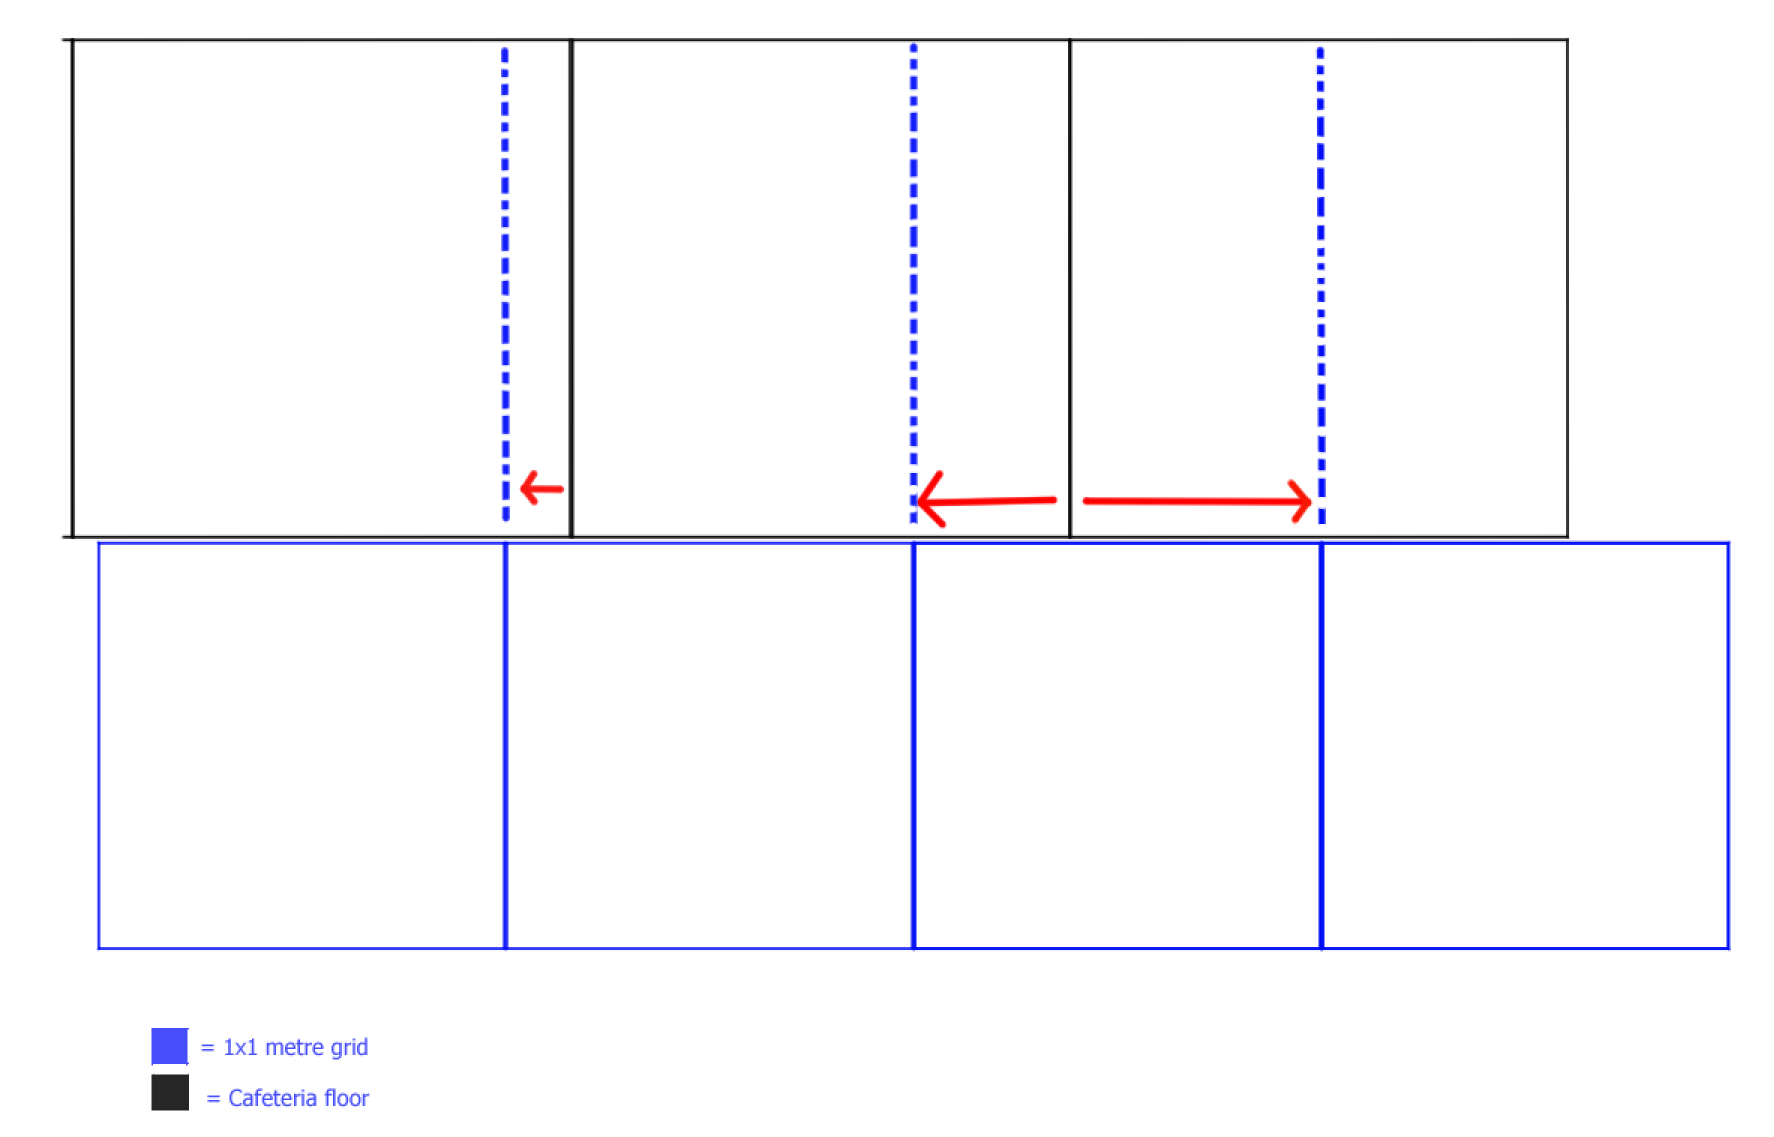
\includegraphics[width=\linewidth]{figures/meth1.png}
        \caption{An Overview of the Research Methodology.}
        \label{fig:research-method}
\end{figure}

\subsection{Identification of Environment Factors}\label{ssec:identification-env-factors}

Environmental factors refer to any physical or logical characteristics of the area used by IPS developers to generate an RSSI-based radio map. In a typical offline map generation phase, the target area is marked and divided into grids that correspond to its digital floor plan and then taped to physically map that area. Each grid is assigned a unique reference number. Data collection is carried out using devices~\cite{add3,add4} capable of measuring RSSI values from various reference points, such as BLE beacons or Wi-Fi access points, at each grid location. The resulting set of RSSI values serves as the feature vector representing each grid (or sub-grid) in the radio map. Sometimes, data synthesis is also used to add more data points from the collected fingerprints~\cite{LRE6}.

From the analysis of the offline map generation process, two key factors emerge as potentially significant to IPS performance. Firstly, grid size directly impacts the precision of position estimation: larger grids make it easier to classify a position into the correct grid, but smaller grids are required for higher positioning accuracy. However, reducing grid size substantially increases the labour required for data collection, rendering map generation impractical for large-scale environments. Secondly, RSSI collection is not strictly limited to reference points~(e.g., access points) within the target area; signals from access points in neighbouring buildings may also be recorded, introducing low-relevance data as shown in Figure~\ref{fig:heatmap}. The x-axis represents the BSSID of different access points, with darker colours indicating lower received signal strength in decibel-meters~(dBm). This study focuses on these two factors as the scope of investigation.

\begin{figure}[th!]
        \centering
        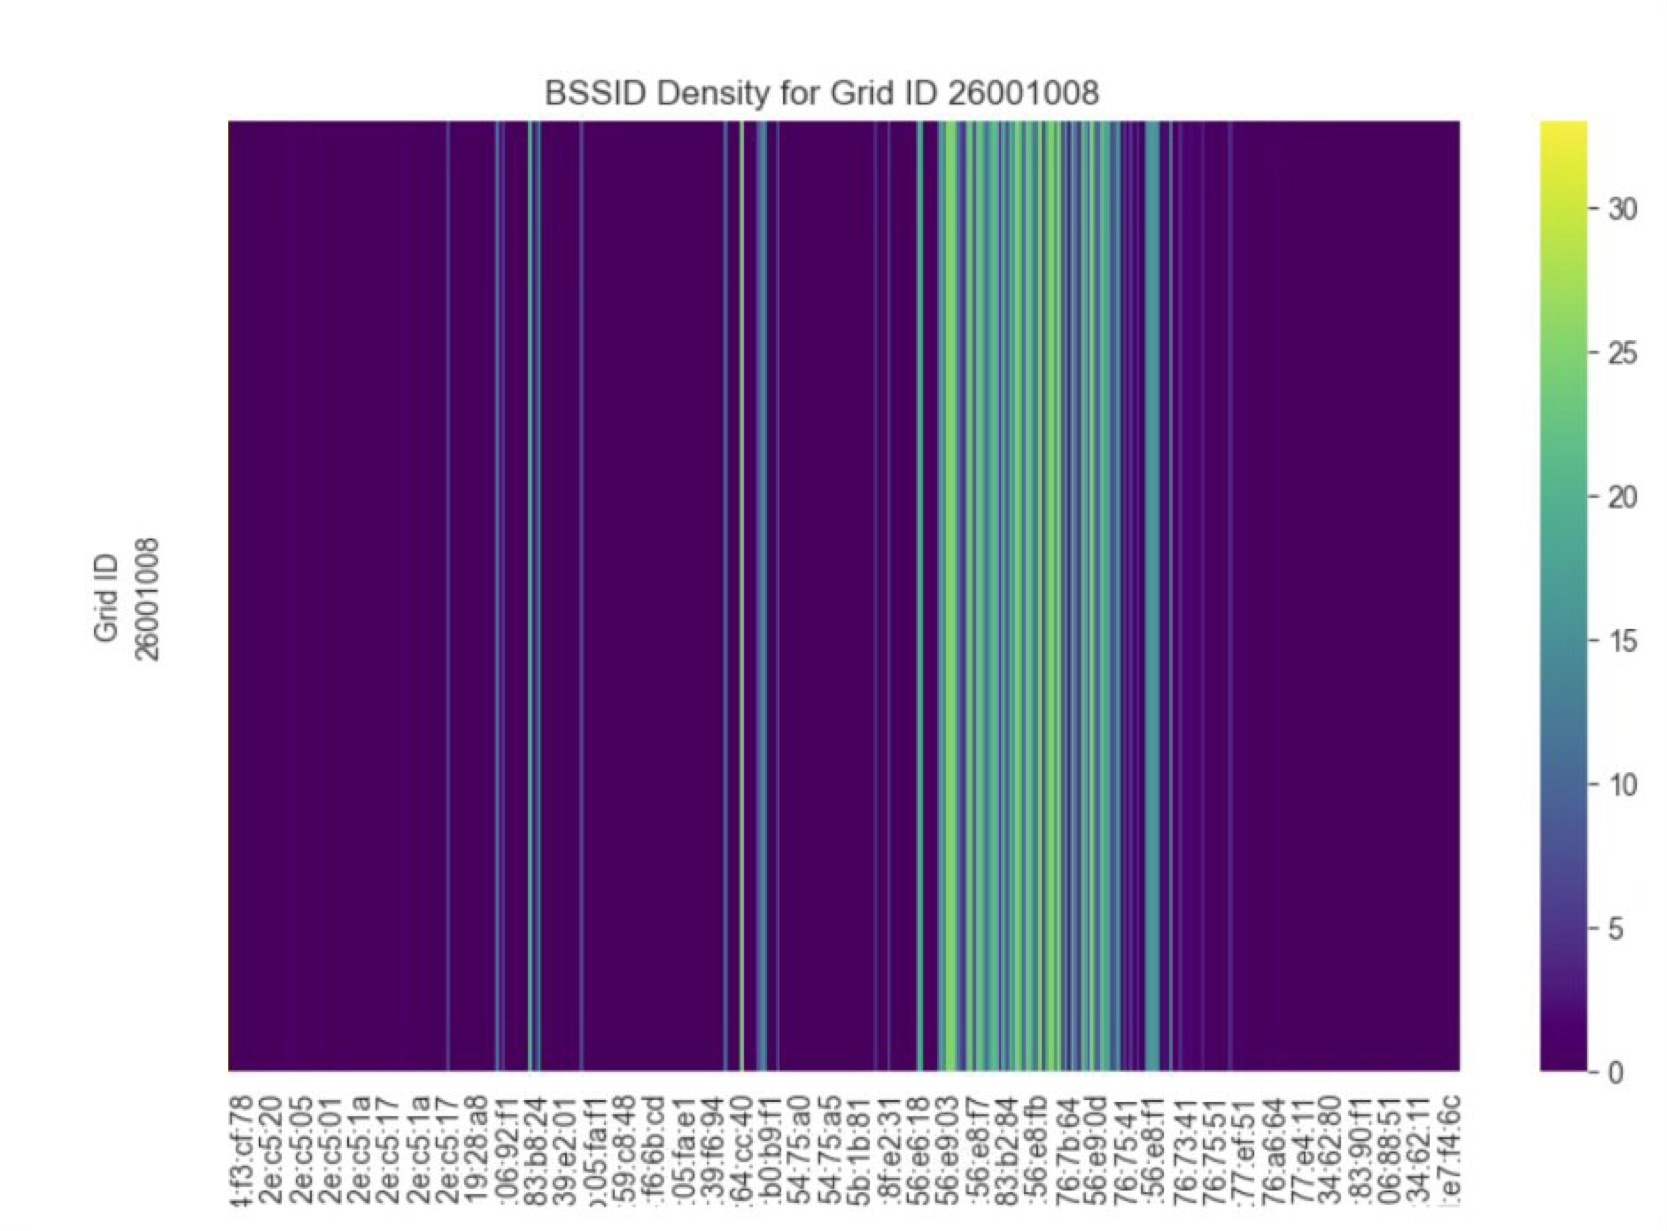
\includegraphics[width=0.7\linewidth]{figures/meth3.jpg}
        \caption{A Heatmap of RSSI values collected from different access points.}
        \label{fig:heatmap}
\end{figure}

\subsection{Extraction of Environmental Factors and Datasets}\label{ssec:extraction}

The two factors identified in the previous section can be tuned, and each is expected to have an optimal balance between practicality and performance. In this section, we extract the quantitative representation of each factor and prepare the dataset for model training and inference accordingly.

For the grid size factor, we quantify it using distance measurements. Traditionally, positioning evaluations rely on precise global coordinates~(e.g., latitude/longitude) as benchmarks. However, such measurements are impractical to obtain indoors without professional surveying equipment. To address this, we introduce two new metrics based on the Euclidean distance concept: Average Grid from Target~(AGT) and Average Distance from Target~(ADT). AGT can be computed using the following equation:
\begin{equation}
        AGT = \sqrt{(x_{target} - x_{estimate})^2 + (y_{target} - y_{estimate})^2}
        \label{eq:agt}
\end{equation}
where $x_{target}$ and $y_{target}$ are the indices of the target grid on the horizontal and vertical axes, respectively, and $x_{estimate}$ and $y_{estimate}$ are the indices of the estimated grid predicted by the IPS. For example, $x_{target} = 3$ and $y_{target} = 5$ indicate that the target grid is the third grid from the left and the fifth grid from the top of the map. By treating grid indices as distance units, this metric naturally adapts to different grid sizes providing both a straightforward means to visualize positioning performance and a standardized measure for cross-comparison across varying grid sizes. 

On the other hand, ADT is a related metric that quantifies the average Euclidean distance, measured in actual physical units such as meters, between the estimated position and the ground-truth target position. It can be computed using the following equation:
\begin{equation}
        ADT = \sqrt{[w_{g} \times (x_{target} - x_{estimate})]^2 + [h_{g} \times (y_{target} - y_{estimate})]^2}
\end{equation}
where $w_{g}$ and $h_{g}$ denote the global grid width and height in meters, respectively. Unlike AGT, which uses grid indices as units, ADT reflects the absolute positioning error in real physical space, making it more interpretable for practical deployment. Notably, larger grid sizes inherently lead to greater distances between the target and the estimated positions, even when the grid index difference remains the same.

On the other hand, quantifying the low-relevance data factor is more straightforward. The performance of an IPS is inversely proportional to the amount of low-relevance data, meaning that the more low-relevance data present, the less accurate the IPS becomes. To identify such data points, we apply a simple threshold-based approach. From the analysis of the collected RSSI heat map in Figure~\ref{fig:heatmap}, it is evident that the majority of low-relevance BSSIDs has its RSSI values fall within the range of 0 to 5 decibel-meters. Based on this observation, we propose using a threshold of 5 decibel-meters to filter out data points that are likely to negatively impact IPS performance.

With the metrics above, we can quantify the effect of different grid sizes in a tangible way. Ideally, data points for various grid sizes should be collected to study the influence of this factor. However, collecting new datasets for each grid size is highly impractical.

In typical IPS experiments, floor taping is used to physically mark grid boundaries, and repeatedly re-taping the same area is extremely time-consuming and prone to human measurement errors.
 
To address this limitation, we propose an interpolation-based approach, where larger grids are generated by aggregating smaller ones. For example, four $1 \times 1$~m grids can be combined into a single $2 \times 2$ m grid, as illustrated in Figure~\ref{fig:vis-grid-aggr}. In each aggregated grid, RSSI values from five sampling points, i.e., top-left, top-right, centre, bottom-left, and bottom-right, are interpolated using a standard averaging method.

\begin{figure}[th!]
        \centering
        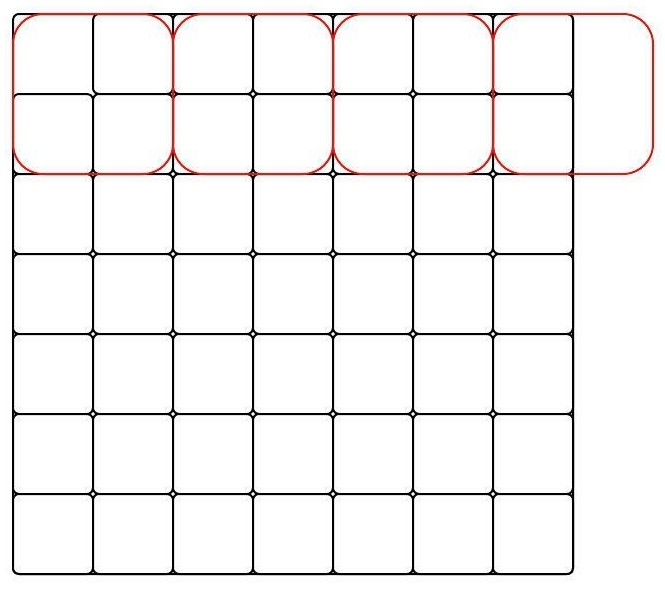
\includegraphics[width=.3\linewidth]{figures/image14.jpg}
        \caption{Visualization of grid aggregation by interpolating RSSI values.}
        \label{fig:vis-grid-aggr}
\end{figure}

A major drawback of the grid interpolation process is the reduction in the number of data points. However, from multiple rounds of data collection in this study, we obtained 9,019 and 3,621 data points from the first- and second-floor hallways, respectively. We believe this is a sufficient number of data points to maintain a high-quality dataset. The difference in the number of data points is due to variations in the floor plan and room partitioning of the test area. Table~\ref{tab:metadata} summarizes the metadata and statistics of the dataset collected in this study.

\begin{table}[th!]
        \caption{Metadata of the number of grids and data points for each grid size.}
        \label{tab:metadata}
        \centering
        \begin{tabular}{|c|l|c|c|c|c|c|c|c|c|}
                \hline
                \multicolumn{2}{|c|}{} & \multicolumn{8}{|c|}{\textbf{Grid Sizes}} \\
                \cline{3-10}
                \multicolumn{2}{|c|}{\textbf{Floor}} & $\mathbf{1\times1}$ & $\mathbf{3\times3}$ & $\mathbf{5\times5}$ & $\mathbf{7\times7}$ & $\mathbf{9\times9}$ & $\mathbf{11\times11}$ & $\mathbf{13\times13}$ & $\mathbf{15\times15}$ \\
                \hline
                \textbf{1st} & \textcolor{blue}{\textbf{\# Grid}} & \textcolor{blue}{309} & \textcolor{blue}{55} & \textcolor{blue}{28} & \textcolor{blue}{17} & \textcolor{blue}{17} & \textcolor{blue}{10} & \textcolor{blue}{10} & \textcolor{blue}{5} \\
                \cline{2-10}
                & \textbf{\# Data Point} & 8,086 & 1,439 & 733 & 445 & 399 & 262 & 235 & 130 \\
                \hline
                \textbf{2nd} & \textcolor{blue}{\textbf{\# Grid}} & \textcolor{blue}{174} & \textcolor{blue}{41} & \textcolor{blue}{19} & \textcolor{blue}{12} & \textcolor{blue}{11} & \textcolor{blue}{6} & \textcolor{blue}{8} & \textcolor{blue}{4} \\
                \cline{2-10}
                & \textbf{\# Data Point} & 4,554 & 1,073 & 497 & 314 & 288 & 157 & 209 & 105 \\
                \hline    
        \end{tabular}
\end{table}

Moreover, the data points in the datasets were analysed to filter out low-relevance features. These features correspond to access points (referred to as BSSIDs), which are a set of RSSI values. Out of the 1,799 BSSIDs initially detected by the data collection device, 1,421 were filtered out as being low-relevance. At this stage, the datasets are ready for the model training process.

\subsection{Model Training}\label{ssec:training}

To study the impact of the identified environmental factors, this paper trains various machine learning models to estimate the current position in terms of the predefined grid layout.

This paper uses four traditional machine learning algorithms (kNN, Random Forest, MLP, and SVM). Additionally, two tree-based ensemble models were selected: XGBoost~\cite{add2} and a hybrid model combining XGBoost + Random Forest. Each model was trained through a standard process, with hyperparameter tuning performed to achieve optimal performance.

The selection of algorithms was based on an analysis of the dataset. We found that each data point contains four main features—the current floor, grid size, current grid index, and a set of corresponding RSSI values—and that most of them are well-structured, sparse, numeric, and ordinal. Therefore, the chosen algorithms needed to be capable of handling and analysing this type of data.


\section{Experiments and Results}\label{sec:experiment-results}

In this section, we conducted experiments to evaluate the performance of various ML algorithms and models on the IPS task. These models were trained as described in Section~\ref{ssec:training}. First, we evaluated the overall performance of the models using key metrics such as accuracy, AGT, and ADT. Afterward, we analyzed the changes in accuracy and AGT that resulted from applying BSSID filtering.

\subsection{Accuracy, AGT, and ADT Results}\label{ssec:acc-agt-adt-results}

Every ML model is trained with the same controlled dataset and workstation. Accuracy, AGT, and ADT are then calculated from the predicted test results compared to the ground truth in the dataset. We plotted graphs to visualize the result comparison between different models and grid sizes based on the accuracy, AGT, and ADT, as shown in Figures~\ref{fig:acc_dgird_size}, \ref{fig:AGT_dgrid_size}, and~\ref{fig:ADT_dgrid_size}.

\begin{figure}[thb!]
	\begin{minipage}{0.45\linewidth}
		\centering
		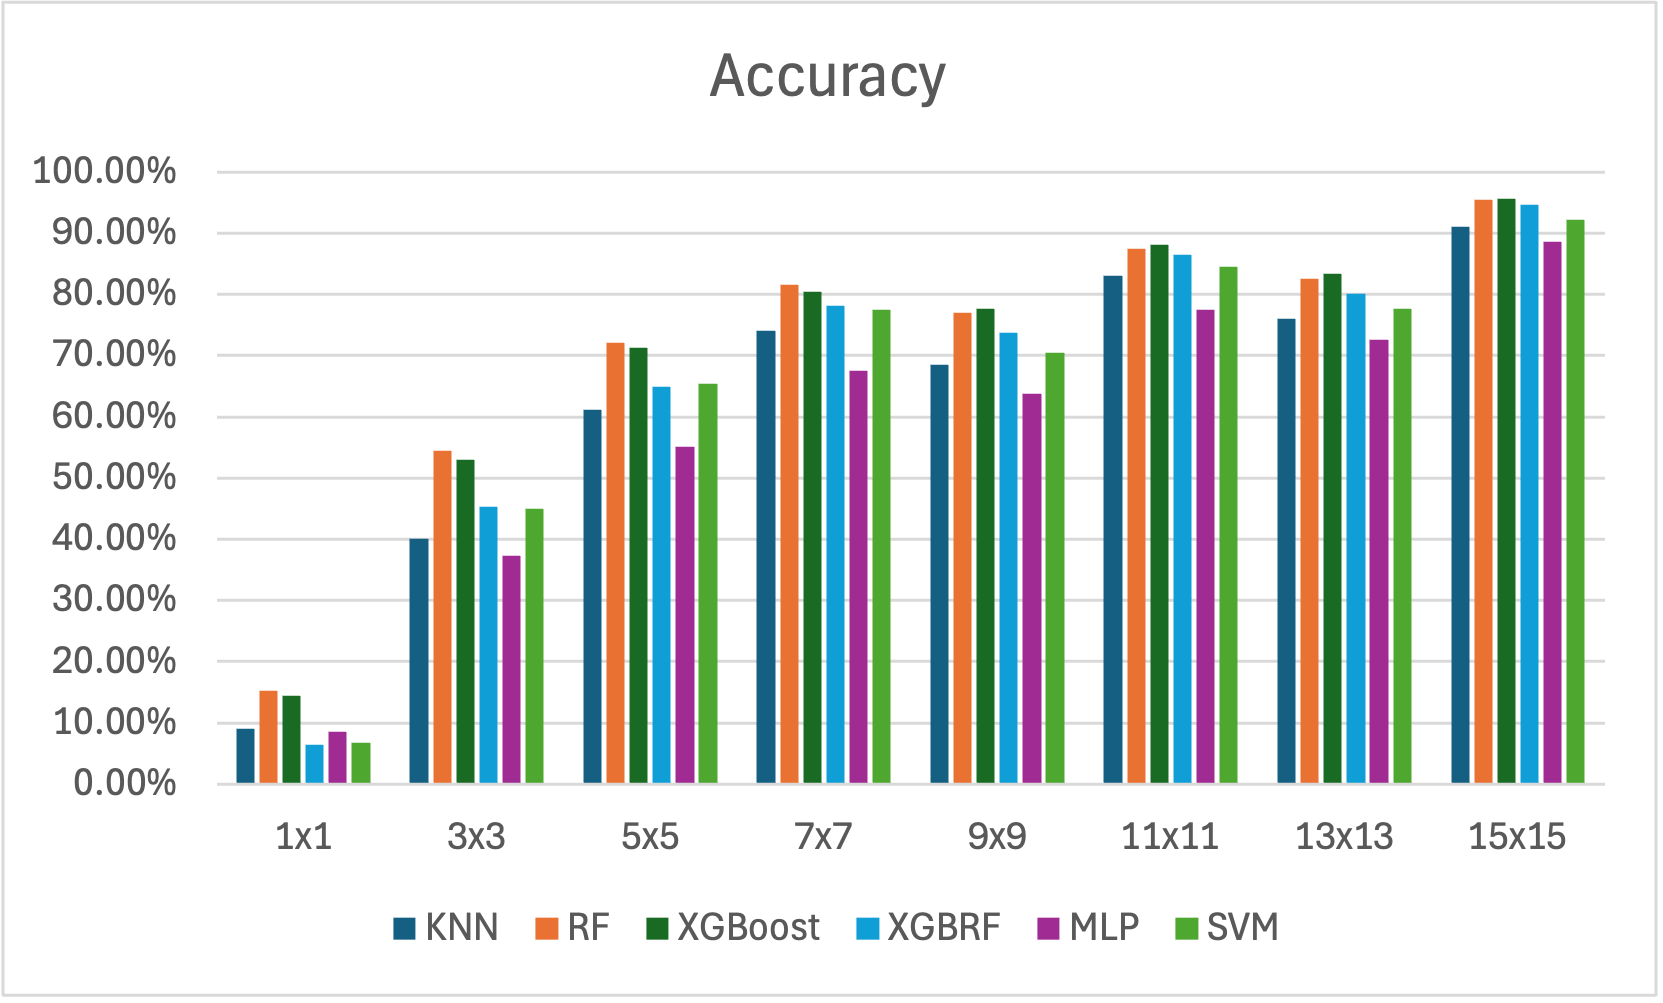
\includegraphics[width=\linewidth]{figures/overview_filtered_accuracy.png}
		\caption{Model Accuracy on Different grid sizes and models (Filtered)}
		\label{fig:acc_dgird_size}
	\end{minipage}
	\hfill
	\begin{minipage}{0.45\linewidth}
		\centering
		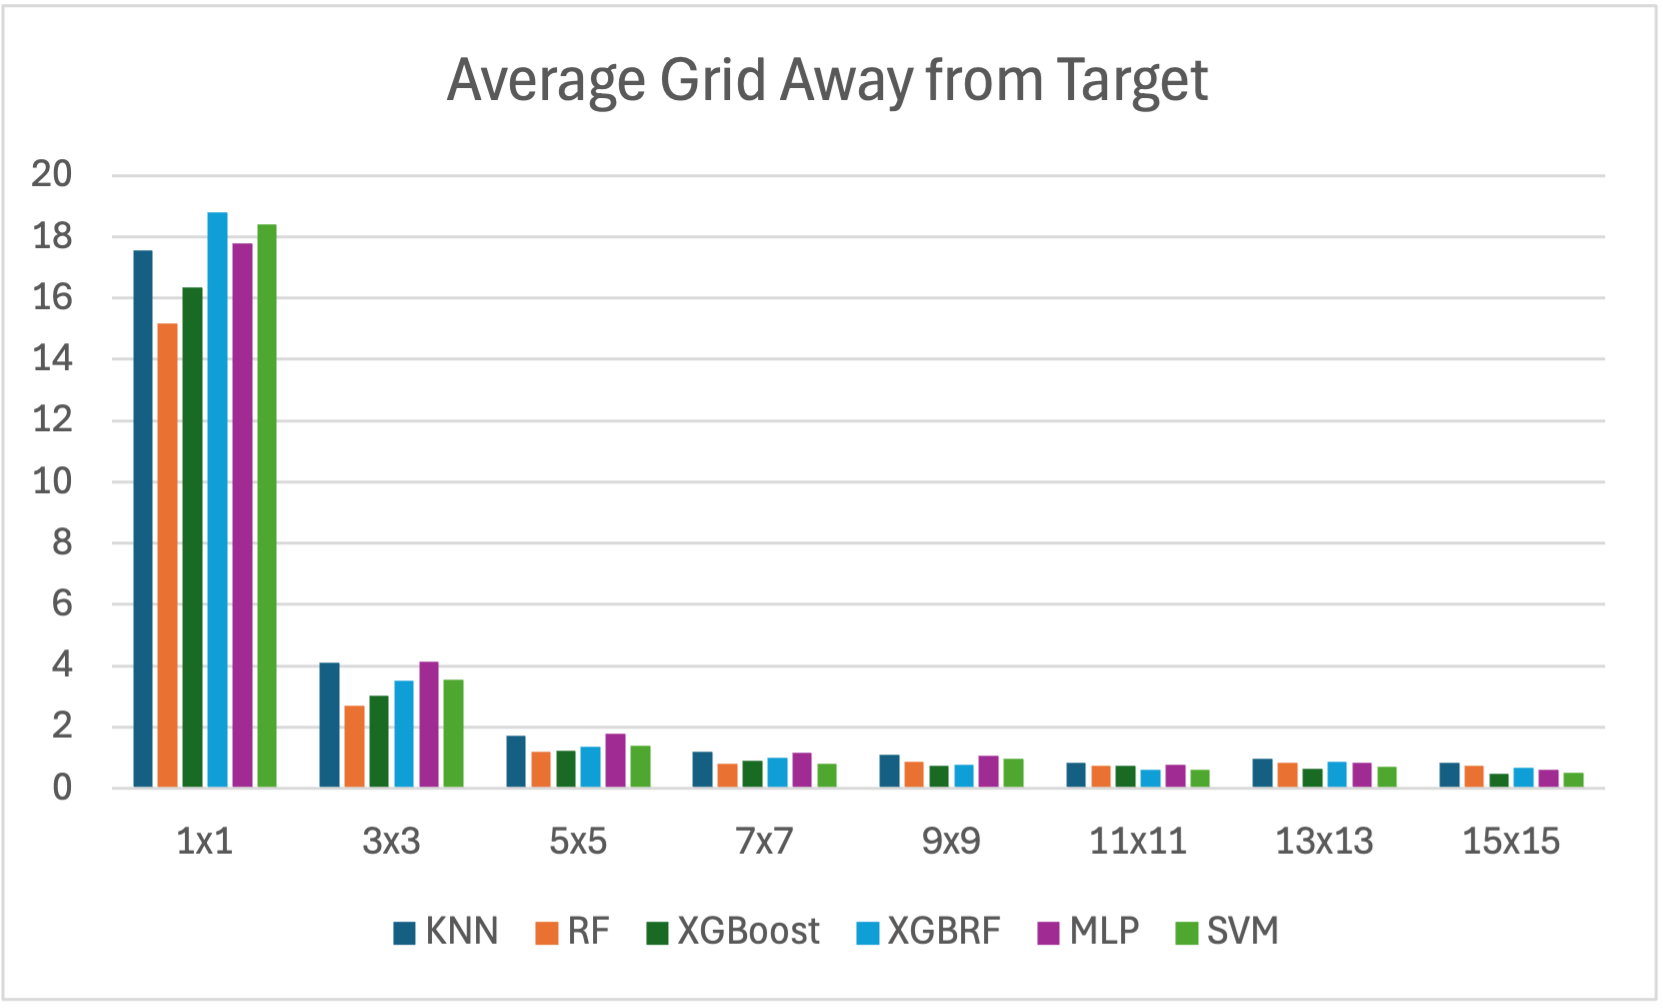
\includegraphics[width=\linewidth]{figures/overview_filtered_agt.png}
		\caption{Model AGT on Different grid sizes and models (Filtered)}
		\label{fig:AGT_dgrid_size}
	\end{minipage}
\end{figure}
\begin{figure}[thb!]
        \centering
        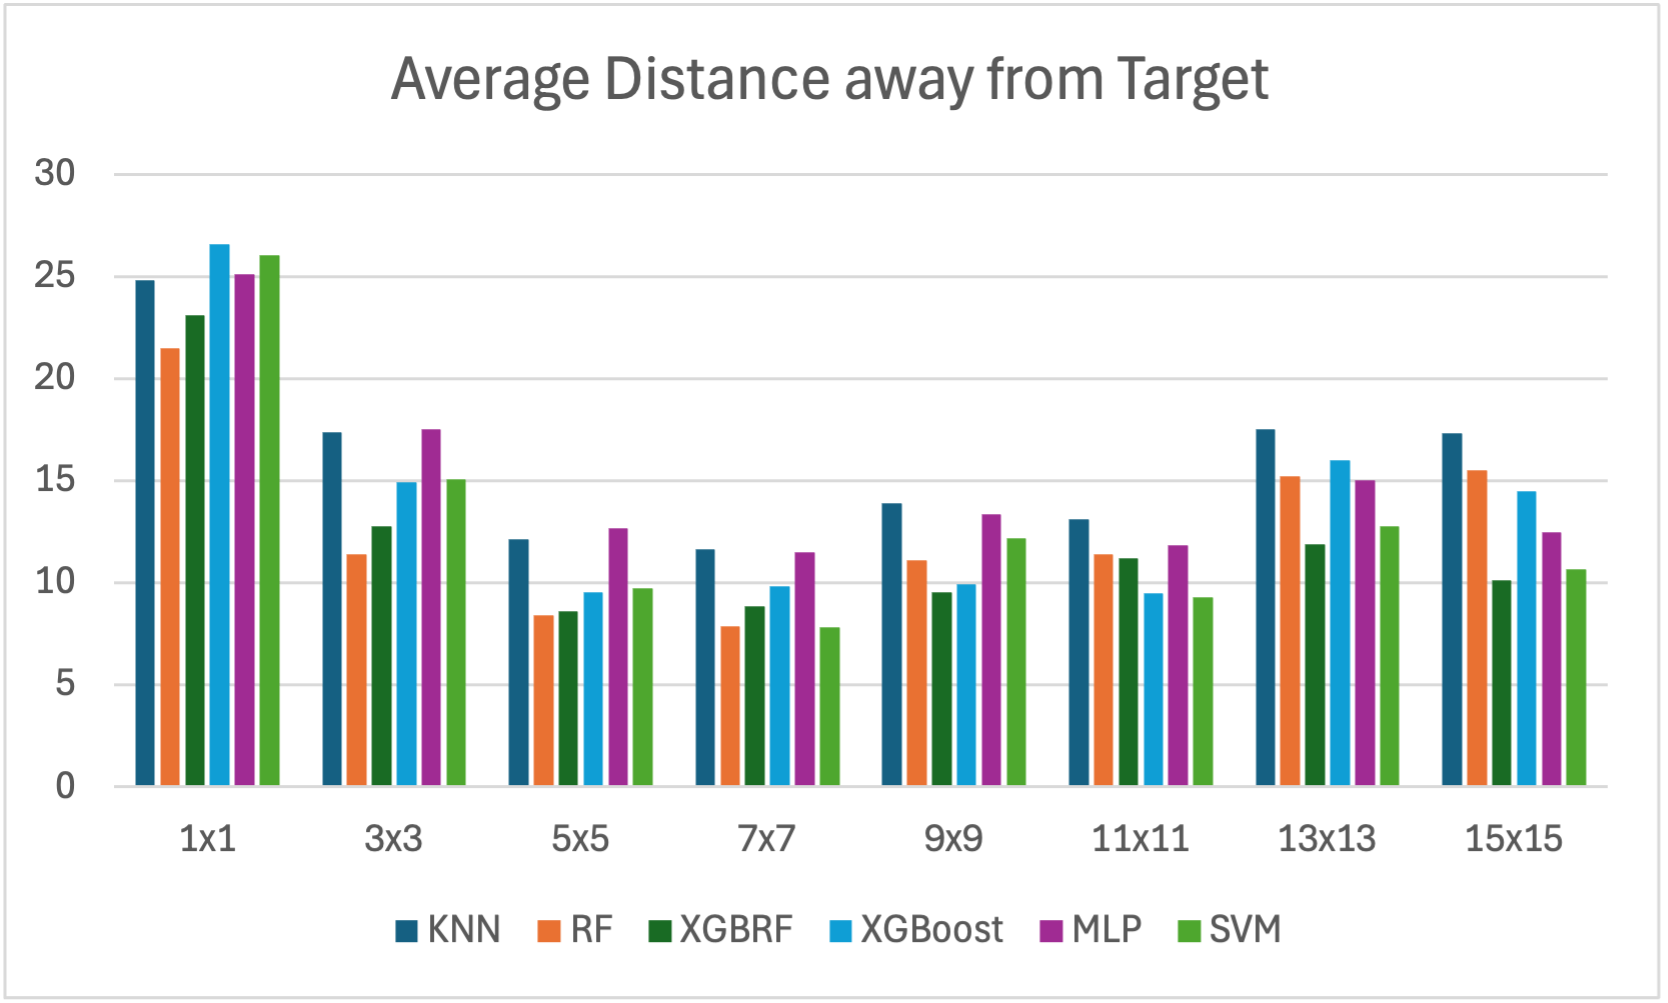
\includegraphics[width=.45\linewidth]{figures/overview_filtered_adt.png}
        \caption{Model ADT on Different grid sizes and models (Filtered)}
        \label{fig:ADT_dgrid_size}
\end{figure}

Figure~\ref{fig:acc_dgird_size} presents the position estimation accuracy of each model across different grid sizes. The results indicate that larger grid sizes generally yield higher accuracy. However, we identified an optimal configuration where the smallest grid size that still achieves high accuracy (approximately 80\%) is $7\times7$m. Additionally, Random Forest (RF) and XGBoost consistently deliver the best performance for position estimation across all grid sizes.

For AGT and ADT in Figures~\ref{fig:AGT_dgrid_size} and~\ref{fig:ADT_dgrid_size}, the results are similar to those for accuracy. Figure~\ref{fig:AGT_dgrid_size} shows that larger grids have lower AGT, meaning it is easier to classify the correct grid during position estimation. The AGT value begins to stabilize once the grid size reaches $7\times7$m, suggesting that this is the smallest grid size capable of maintaining minimal errors. On the other hand, Figure~\ref{fig:ADT_dgrid_size} indicates that a $7\times7$m grid size minimizes error while remaining small enough for precision-dependent applications in this specific setting. The ADT results confirm that, even when measured in physical units, the $7\times7$m grid size remains the optimal point.

\subsection{Filtering Impact on Model Performance}\label{ssec:filtering-impact}

As described in Section~\ref{ssec:extraction}, BSSID filtering is proposed to exclude low-relevance data from the dataset. This approach can reduce computational resource requirements, particularly in scenarios with a large feature space (i.e., a high number of BSSIDs within the area network). To evaluate whether this filtering process can improve IPS performance, we conducted experiments comparing all models trained on datasets generated with and without filtering across all grid sizes.

\begin{figure}[tbh!]
	\centering
	\begin{minipage}{0.45\linewidth}
		\centering
		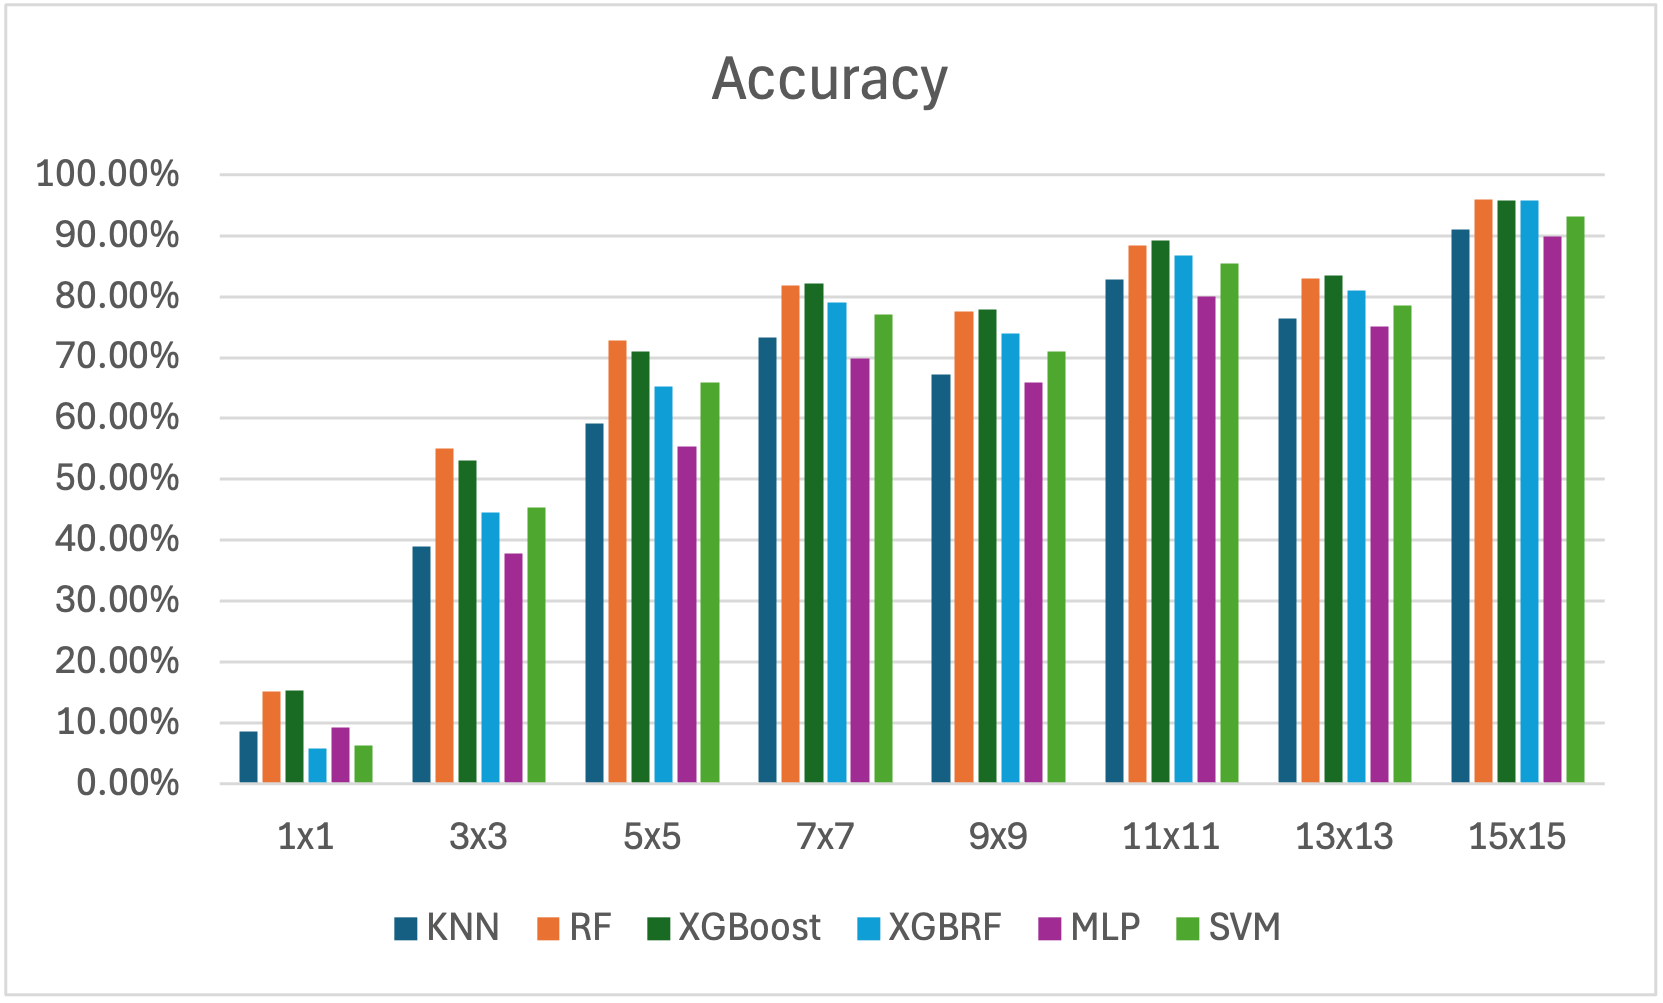
\includegraphics[width=\linewidth]{figures/overview_unfiltered_accuracy.png}
		\caption{Model Accuracy (Unfiltered)}
		\label{fig:acc_unfiltered}
	\end{minipage}
	\hfill
	\begin{minipage}{0.45\linewidth}
		\centering
		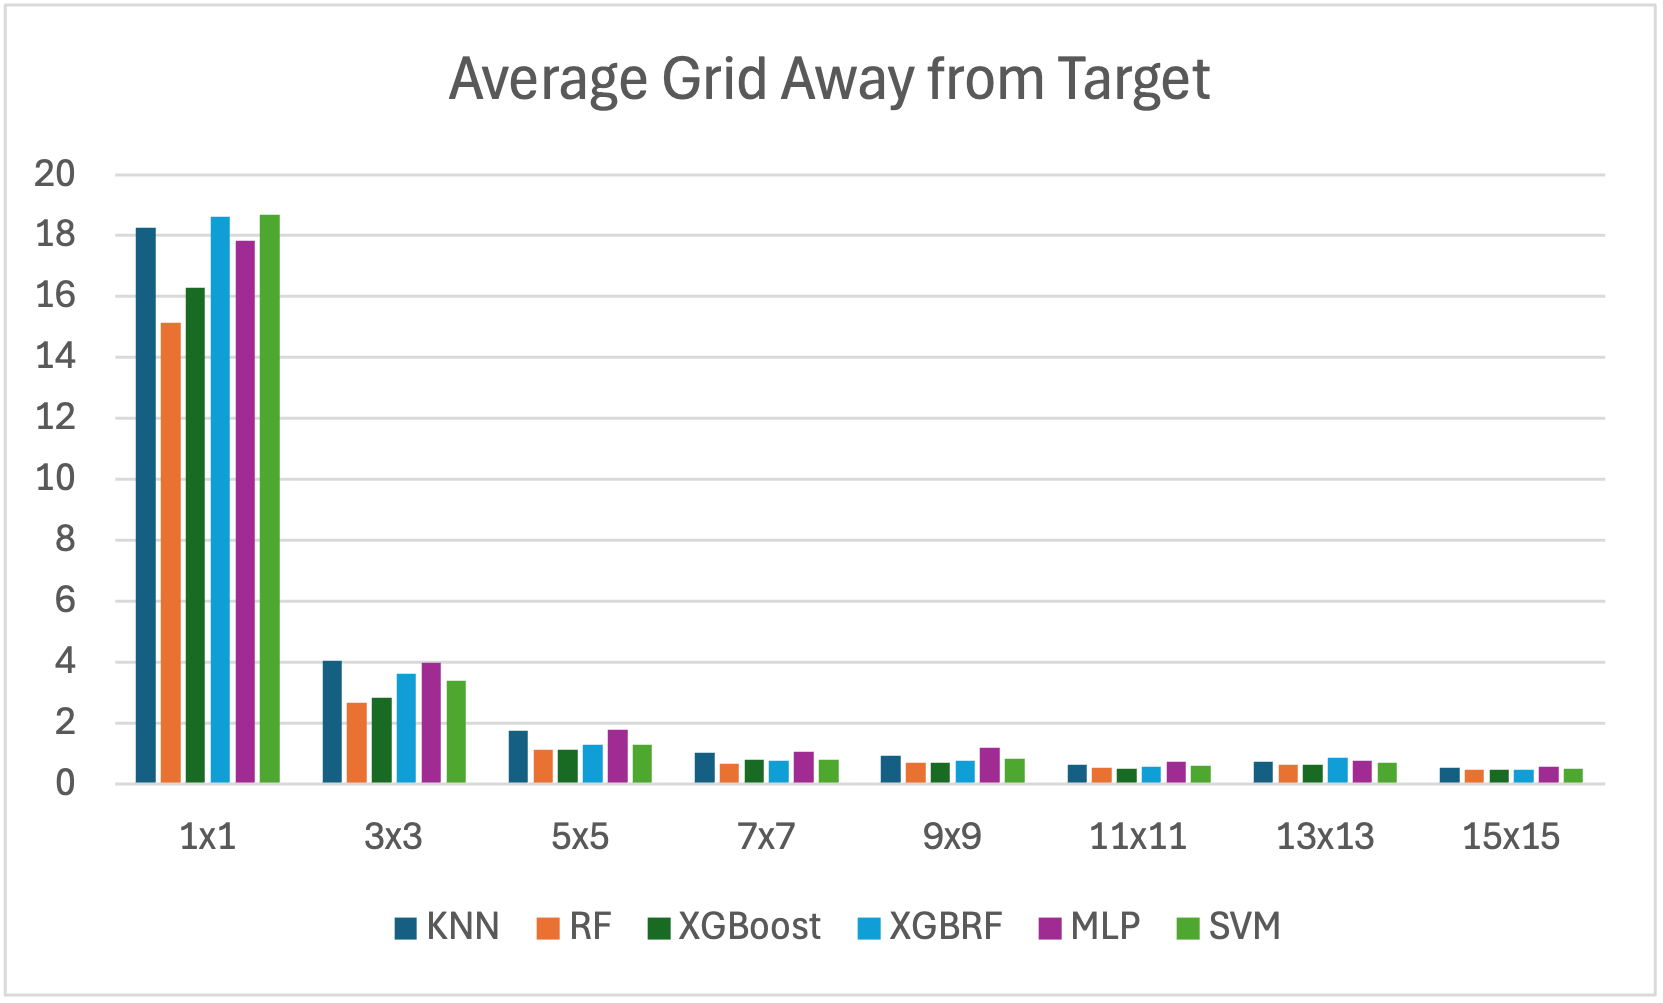
\includegraphics[width=\linewidth]{figures/overview_unfiltered_agt.png}
		\caption{Model AGT (Unfiltered)}
		\label{fig:agt_unfiltered}
	\end{minipage}
\end{figure}

\begin{figure}[tbh!]
	\centering
	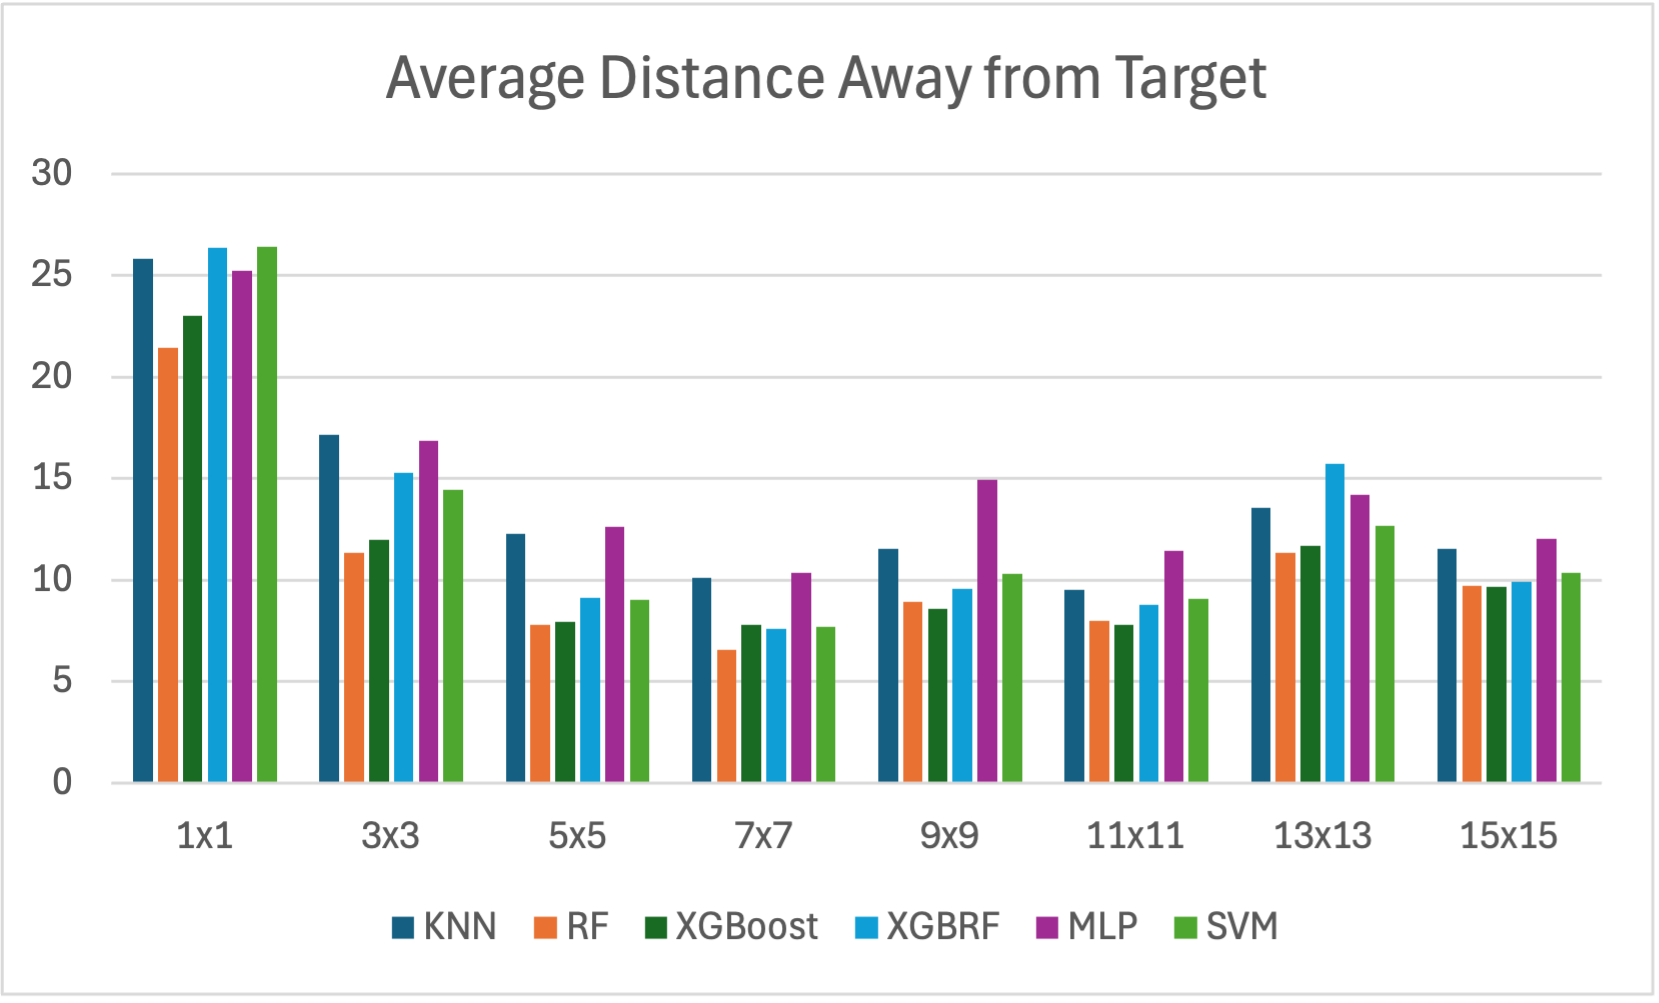
\includegraphics[width=.45\linewidth]{figures/overview_unfiltered_adt.png}
	\caption{Model ADT (Unfiltered)}
	\label{fig:adt_unfiltered}
\end{figure}

Comparing Figures~\ref{fig:acc_dgird_size} and~\ref{fig:acc_unfiltered} reveals the impact of BSSID filtering on model accuracy across all models and grid sizes. The filtered dataset (Figure~\ref{fig:acc_dgird_size}) shows consistently higher accuracy across most models and grid configurations compared to the unfiltered dataset (Figure~\ref{fig:acc_unfiltered}). Similarly, Figures~\ref{fig:AGT_dgrid_size} and~\ref{fig:agt_unfiltered} demonstrate that filtering reduces AGT values, indicating improved positioning precision. The ADT comparison (Figures~\ref{fig:ADT_dgrid_size} and~\ref{fig:adt_unfiltered}) further confirms that filtering enhances overall model performance while significantly reducing computational requirements by decreasing the feature space from 1799 to 378 BSSIDs.

\section{Discussion}\label{sec:discussion}

This study investigated the optimization of multi-floor IPS through a systematic evaluation of environmental factors influencing fingerprinting performance when using ML approaches. The analysis focused on two main factors: the grid size for fingerprint data collection and the impact of low-relevance BSSIDs in the area network. Through extensive experimentation across different grid sizes, several key insights emerged.

First, grid size was found to have a substantial impact on model performance across all evaluation metrics. Contrary to the common assumption that smaller grid sizes always enhance precision, our findings indicate that a moderate grid size, specifically $7\times7$m, strikes the best balance between spatial resolution and positioning precision. Models trained on this grid size consistently achieved the highest accuracy (approximately 80\%), along with the lowest AGT and ADT values. This suggests that while finer grids may provide more data points, they also introduce variability that can overwhelm ML models without delivering proportional gains in localization accuracy.

Second, the analysis of filtering low-relevance BSSIDs showed only marginal improvements. While excluding low-intensity signals (e.g., -100 dBm from distant or low-relevance access points) slightly enhanced accuracy and reduced AGT, the gains were minimal. This indicates that although data cleaning contributes to input quality, the spatial configuration of data—particularly grid structuring—plays a more dominant role in IPS performance for multi-floor environments.

Among the ML models evaluated, RF and XGBoost consistently delivered superior performance across all metrics and grid configurations. These ensemble methods appear well-suited to the fingerprint-matching task, likely due to their ability to capture complex feature interactions and resist overfitting, particularly in environments with noisy or redundant RSSI signals. Interestingly, more complex deep learning models, such as MLP, did not outperform these simpler ML techniques, supporting the view that in settings with constrained or moderately sized datasets, traditional models can offer a better trade-off between accuracy and computational efficiency.

It is important to contextualize the generalizability of our findings. The test environment, which is a university campus building with realistic multi-floor usage, ensures ecological validity, but certain parameters (e.g., architectural layout, number of access points, and building materials) are inherently site-specific. As such, while the identified optimal grid size and preferred models provide valuable guidance, they may require recalibration for different environments such as warehouses, shopping malls, or hospitals.

Finally, the proposed methodology of using interpolation to synthesize multiple grid sizes from a single fine-grained dataset substantially reduces the labour intensiveness of traditional IPS data collection. This approach not only improves reproducibility and scalability but also establishes a practical framework for future IPS research to systematically explore environmental configurations.

\section{Conclusion and Future Directions}\label{sec:conclusion}

This study explored the optimization of multi-floor IPS using grid-based fingerprinting and machine learning. By systematically analysing the impact of grid size and the RSSI values of low-relevance BSSIDs on IPS performance, we identified that a grid size of $7\times7$m offers the best balance between accuracy and practicality of data collection. Our findings demonstrated that ensemble-based ML models such as RF and XGBoost consistently outperformed other algorithms, achieving high accuracy and low prediction error across multiple evaluation metrics. While filtering out low-relevance BSSIDs and their RSSI values slightly improved model performance, the overall influence was modest, suggesting that strategic spatial structuring has a more significant effect on accuracy than simple data cleaning.

Looking forward, there are several directions for future research. First, exploring more advanced deep learning models, such as attention-based networks or hybrid GNN-MLP architectures, could uncover further performance gains, especially when trained on larger and more diverse datasets. Additionally, implementing real-time IPS applications with adaptive grid configurations may help tailor accuracy to user needs in dynamic environments. Finally, future work may also examine the use of synthetic data augmentation, sensor fusion, and transfer learning approaches to improve generalization across different buildings or floors.

%
% ---- Bibliography ----
%
\bibliographystyle{splncs04}
\bibliography{references}

\newpage

\appendix

\section*{Appendix}

\section{Implementation Details: Grid Alignment Challenges}

During the data collection phase, several practical challenges emerged that required careful consideration.

\begin{figure}[!tbph]
	\centering
	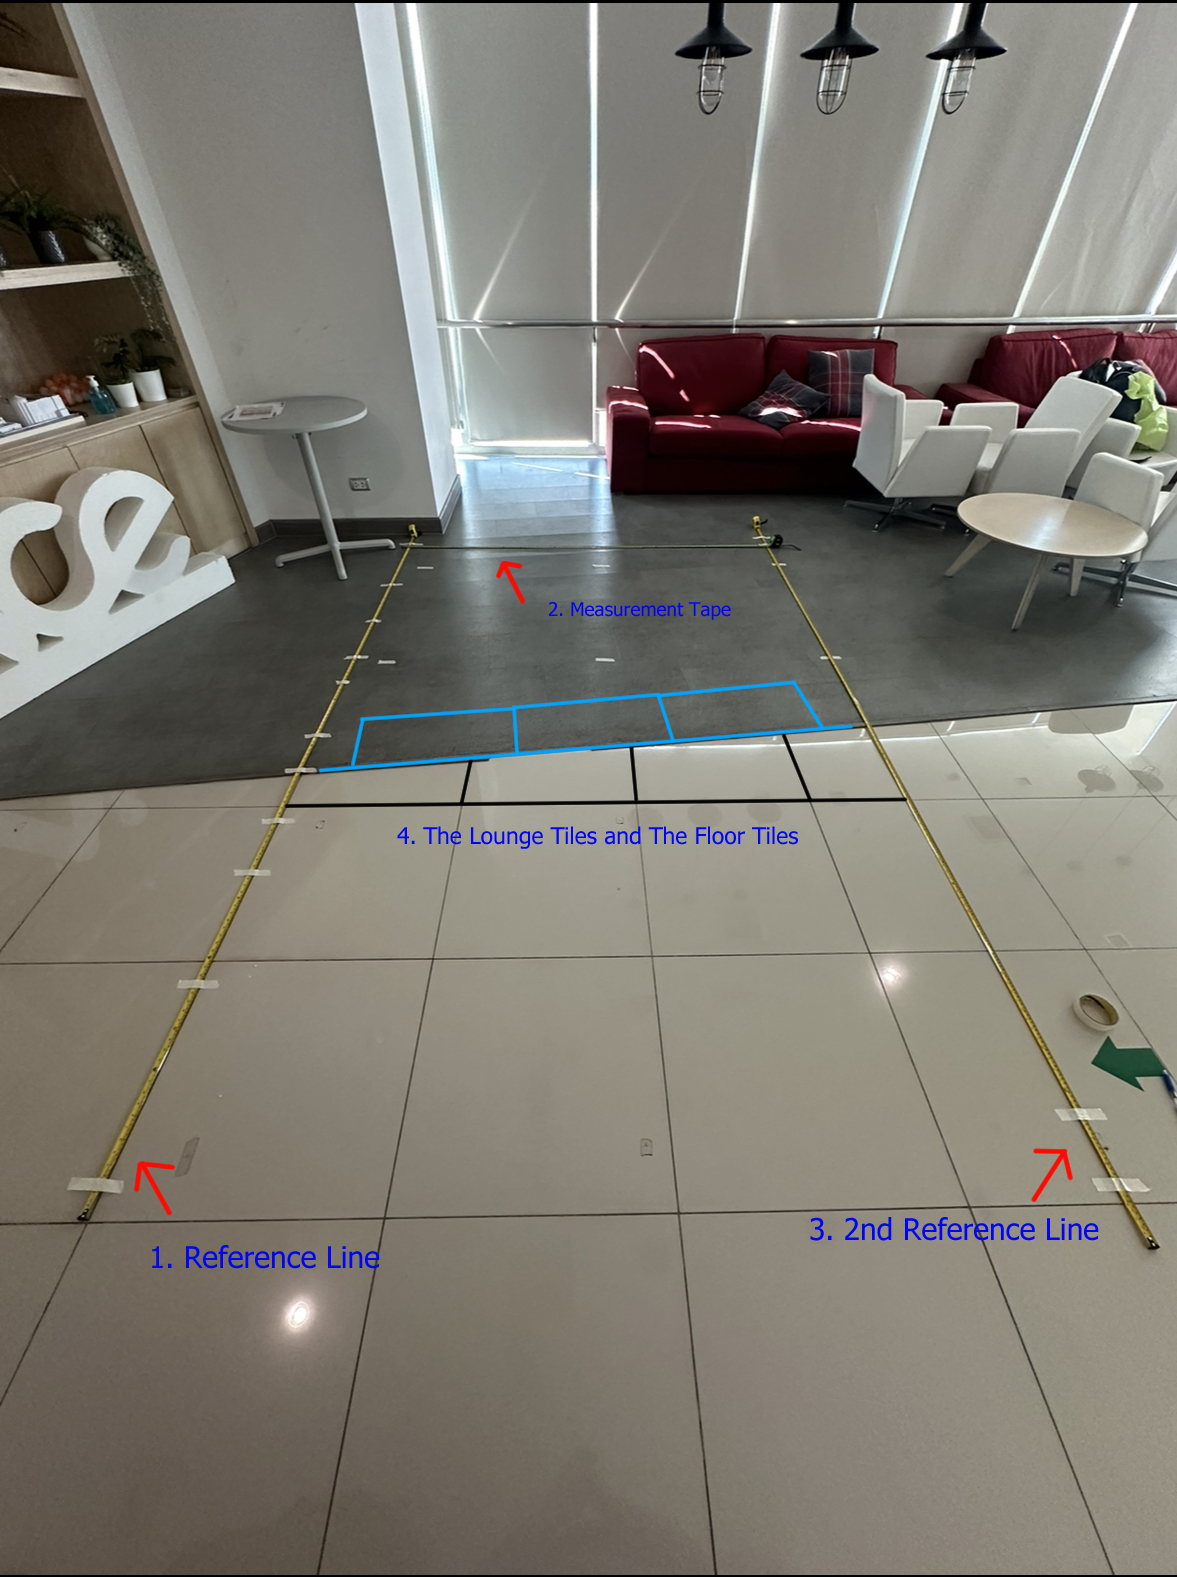
\includegraphics[width=\textwidth]{figures/meth2.jpg}
	\caption{An example of taping that was done to create grids for data collection of RSSI values as fingerprints}
	\label{fig:taping}
\end{figure}

\subsection{Floor Tiling Variations}
Different layouts and tiling across areas presented challenges, as certain floors had distinct tiling with varying elevations and angles (as shown in Fig. \ref{fig:taping}). This was addressed by constructing grids based on previous reference points. Although minor measurement inaccuracies may exist, they are negligible for the purposes of this study.

\subsection{Edge Grid Effects}
While taping and collecting data points, another factor that could interfere with the IPS collection presented itself. The specific area inside the grid also affected how many RSSI values were present. For instance, collecting data in the top left corner of the grid could produce different RSSI values compared to the center of the grid. 

This issue could be addressed by either (1) removing the edge grids or (2) collecting fewer data points in the edge grid. However, both methods result in fewer data points being collected and have minimal impact on IPS performance. This is based on the assumption that, from a user experience perspective, being located at the edge of a grid represents a transitional state between adjacent grids. Meaning that, if misclassification occurs, it typically involves the neighboring grid and the correct grid itself. Therefore, for this study, the edge grid factor is negligible and omitted from further analysis.

\section{Hardware Implementation Considerations}
During the experimentation phase, specific hardware limitations significantly impacted the feasibility of training models with different feature sets. When attempting to train on the full, unfiltered BSSID set (1799 features), computational demands quickly became impractical—the RTX 3080 Ti GPU struggled even with the smallest grid size configurations. Although exact runtimes were not recorded, the difference in resource demands between filtered and unfiltered datasets was substantial.

By applying the simple filtering approach that reduced features from 1799 to 378 BSSIDs, model training became feasible across the entire range of grid sizes (1×1 to 15×15). This hardware constraint, while limiting, provided valuable insights into the practical utility of the full feature set and suggests that systematic feature selection or dimensionality reduction studies could be worthwhile in future work. The filtering approach not only made training computationally feasible but also demonstrated that selective feature reduction can maintain or even improve model performance while significantly reducing computational requirements.

\section{Detailed Model Performance Analysis}

This section provides comprehensive performance comparisons for all machine learning models evaluated in this study across key grid sizes (1×1m, 7×7m, and 15×15m). The analysis includes side-by-side comparisons of accuracy and custom metric (AGT) measurements for both filtered and unfiltered BSSID datasets. These detailed results address the comparative performance of kNN, MLP, SVM, XGBoost, and XGBoost Random Forest models across different feature sets.

\subsection*{kNN}

\begin{figure}[H]
	\centering
	\begin{minipage}{0.49\textwidth}
		\centering
		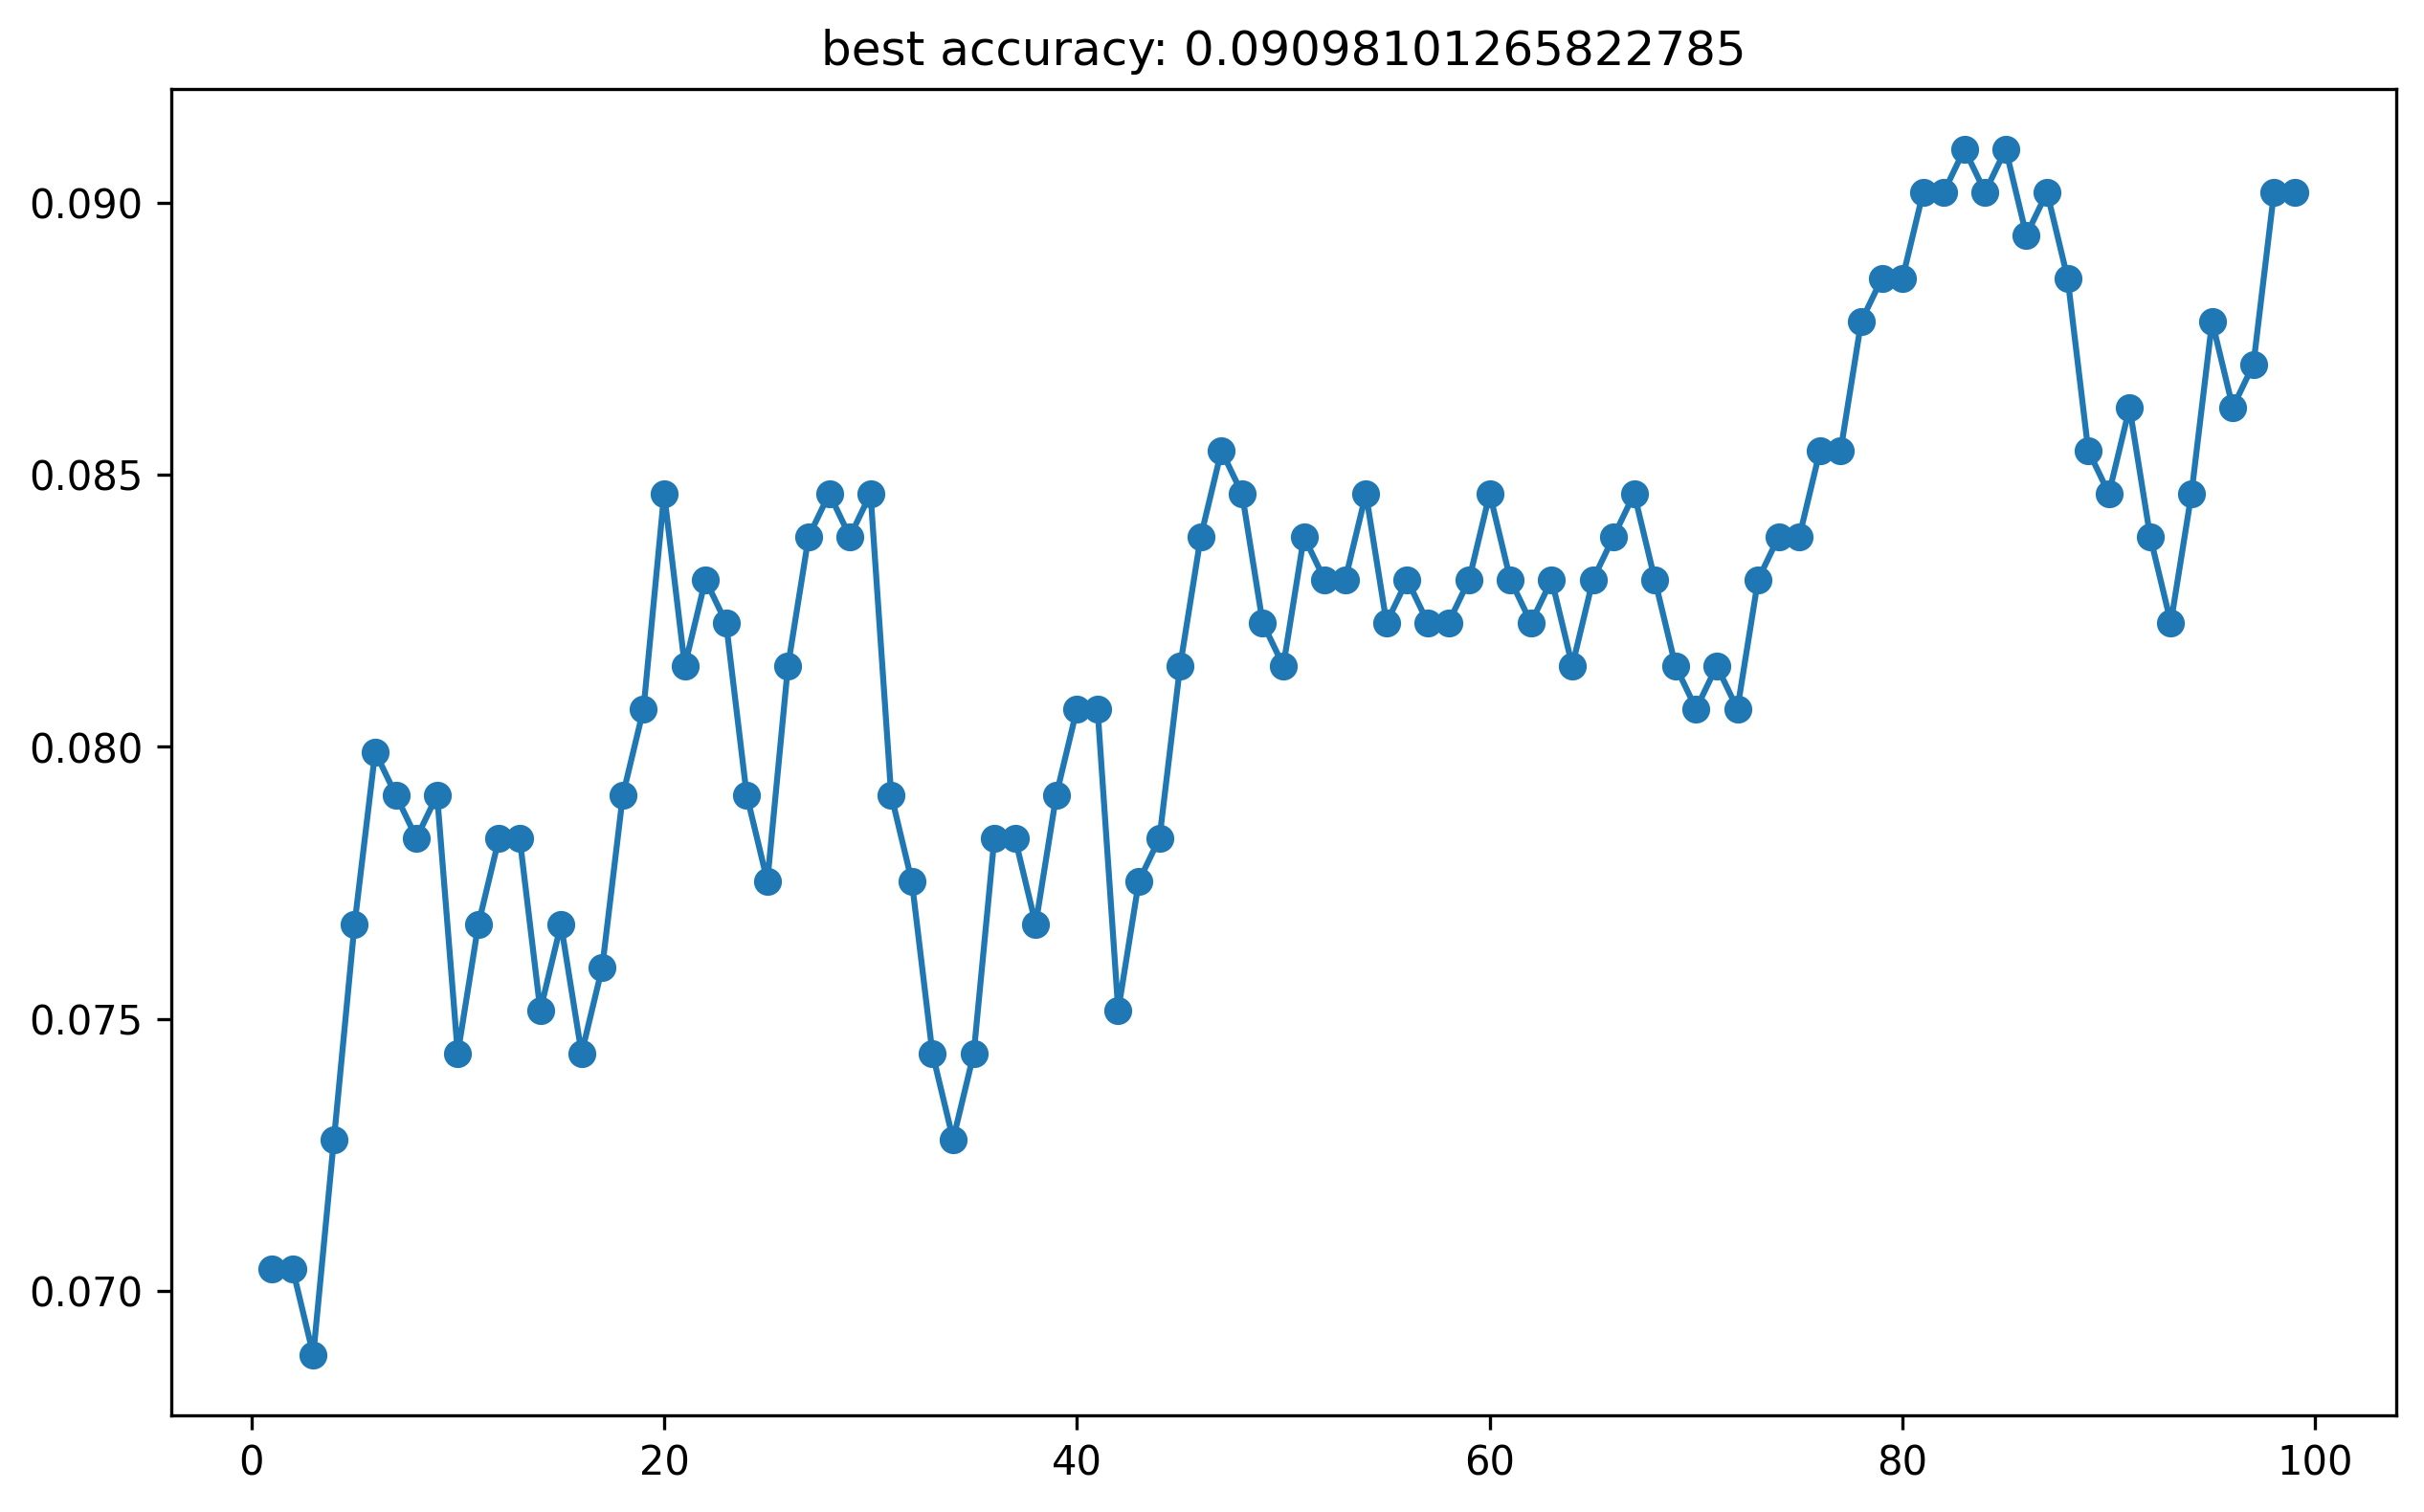
\includegraphics[width=\textwidth]{figures/filtered/knn_acc_1.png}
		\caption*{Accuracy (Filtered): 1×1m}
	\end{minipage}
	\hfill
	\begin{minipage}{0.49\textwidth}
		\centering
		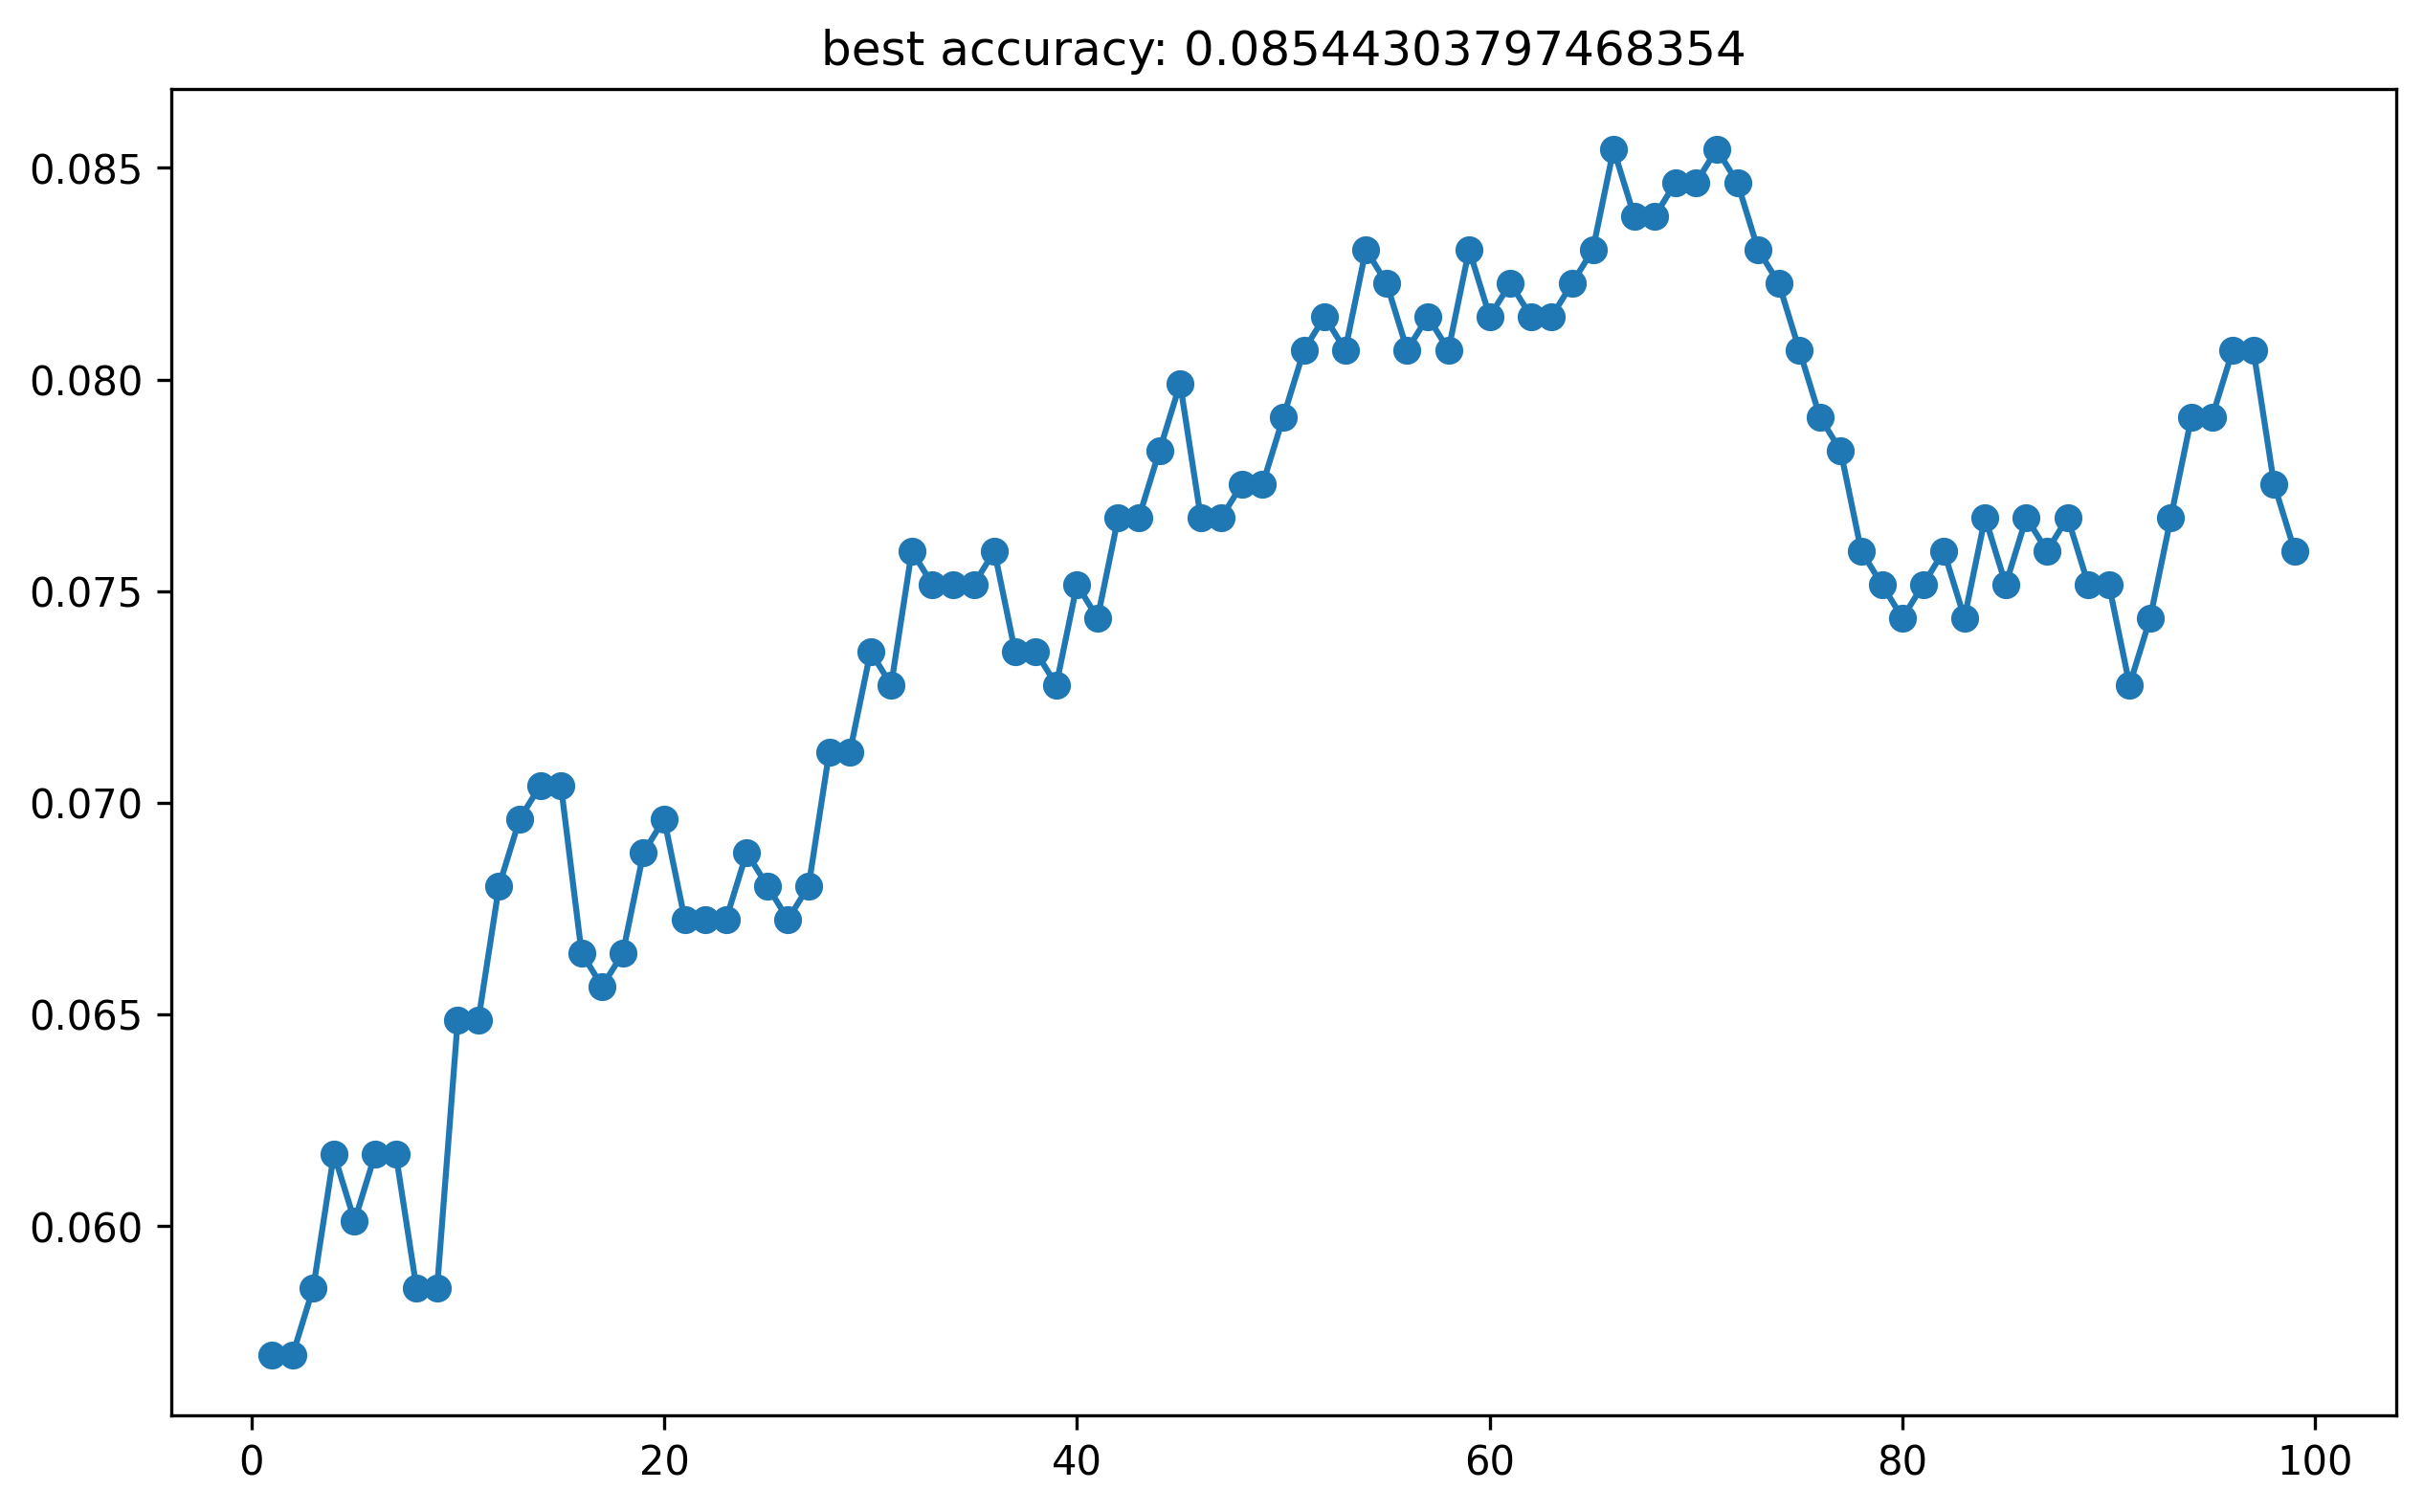
\includegraphics[width=\textwidth]{figures/unfiltered/knn_acc_1.png}
		\caption*{Accuracy (Unfiltered): 1×1m}
	\end{minipage}
\end{figure}

\begin{figure}[H]
	\centering
	\begin{minipage}{0.49\textwidth}
		\centering
		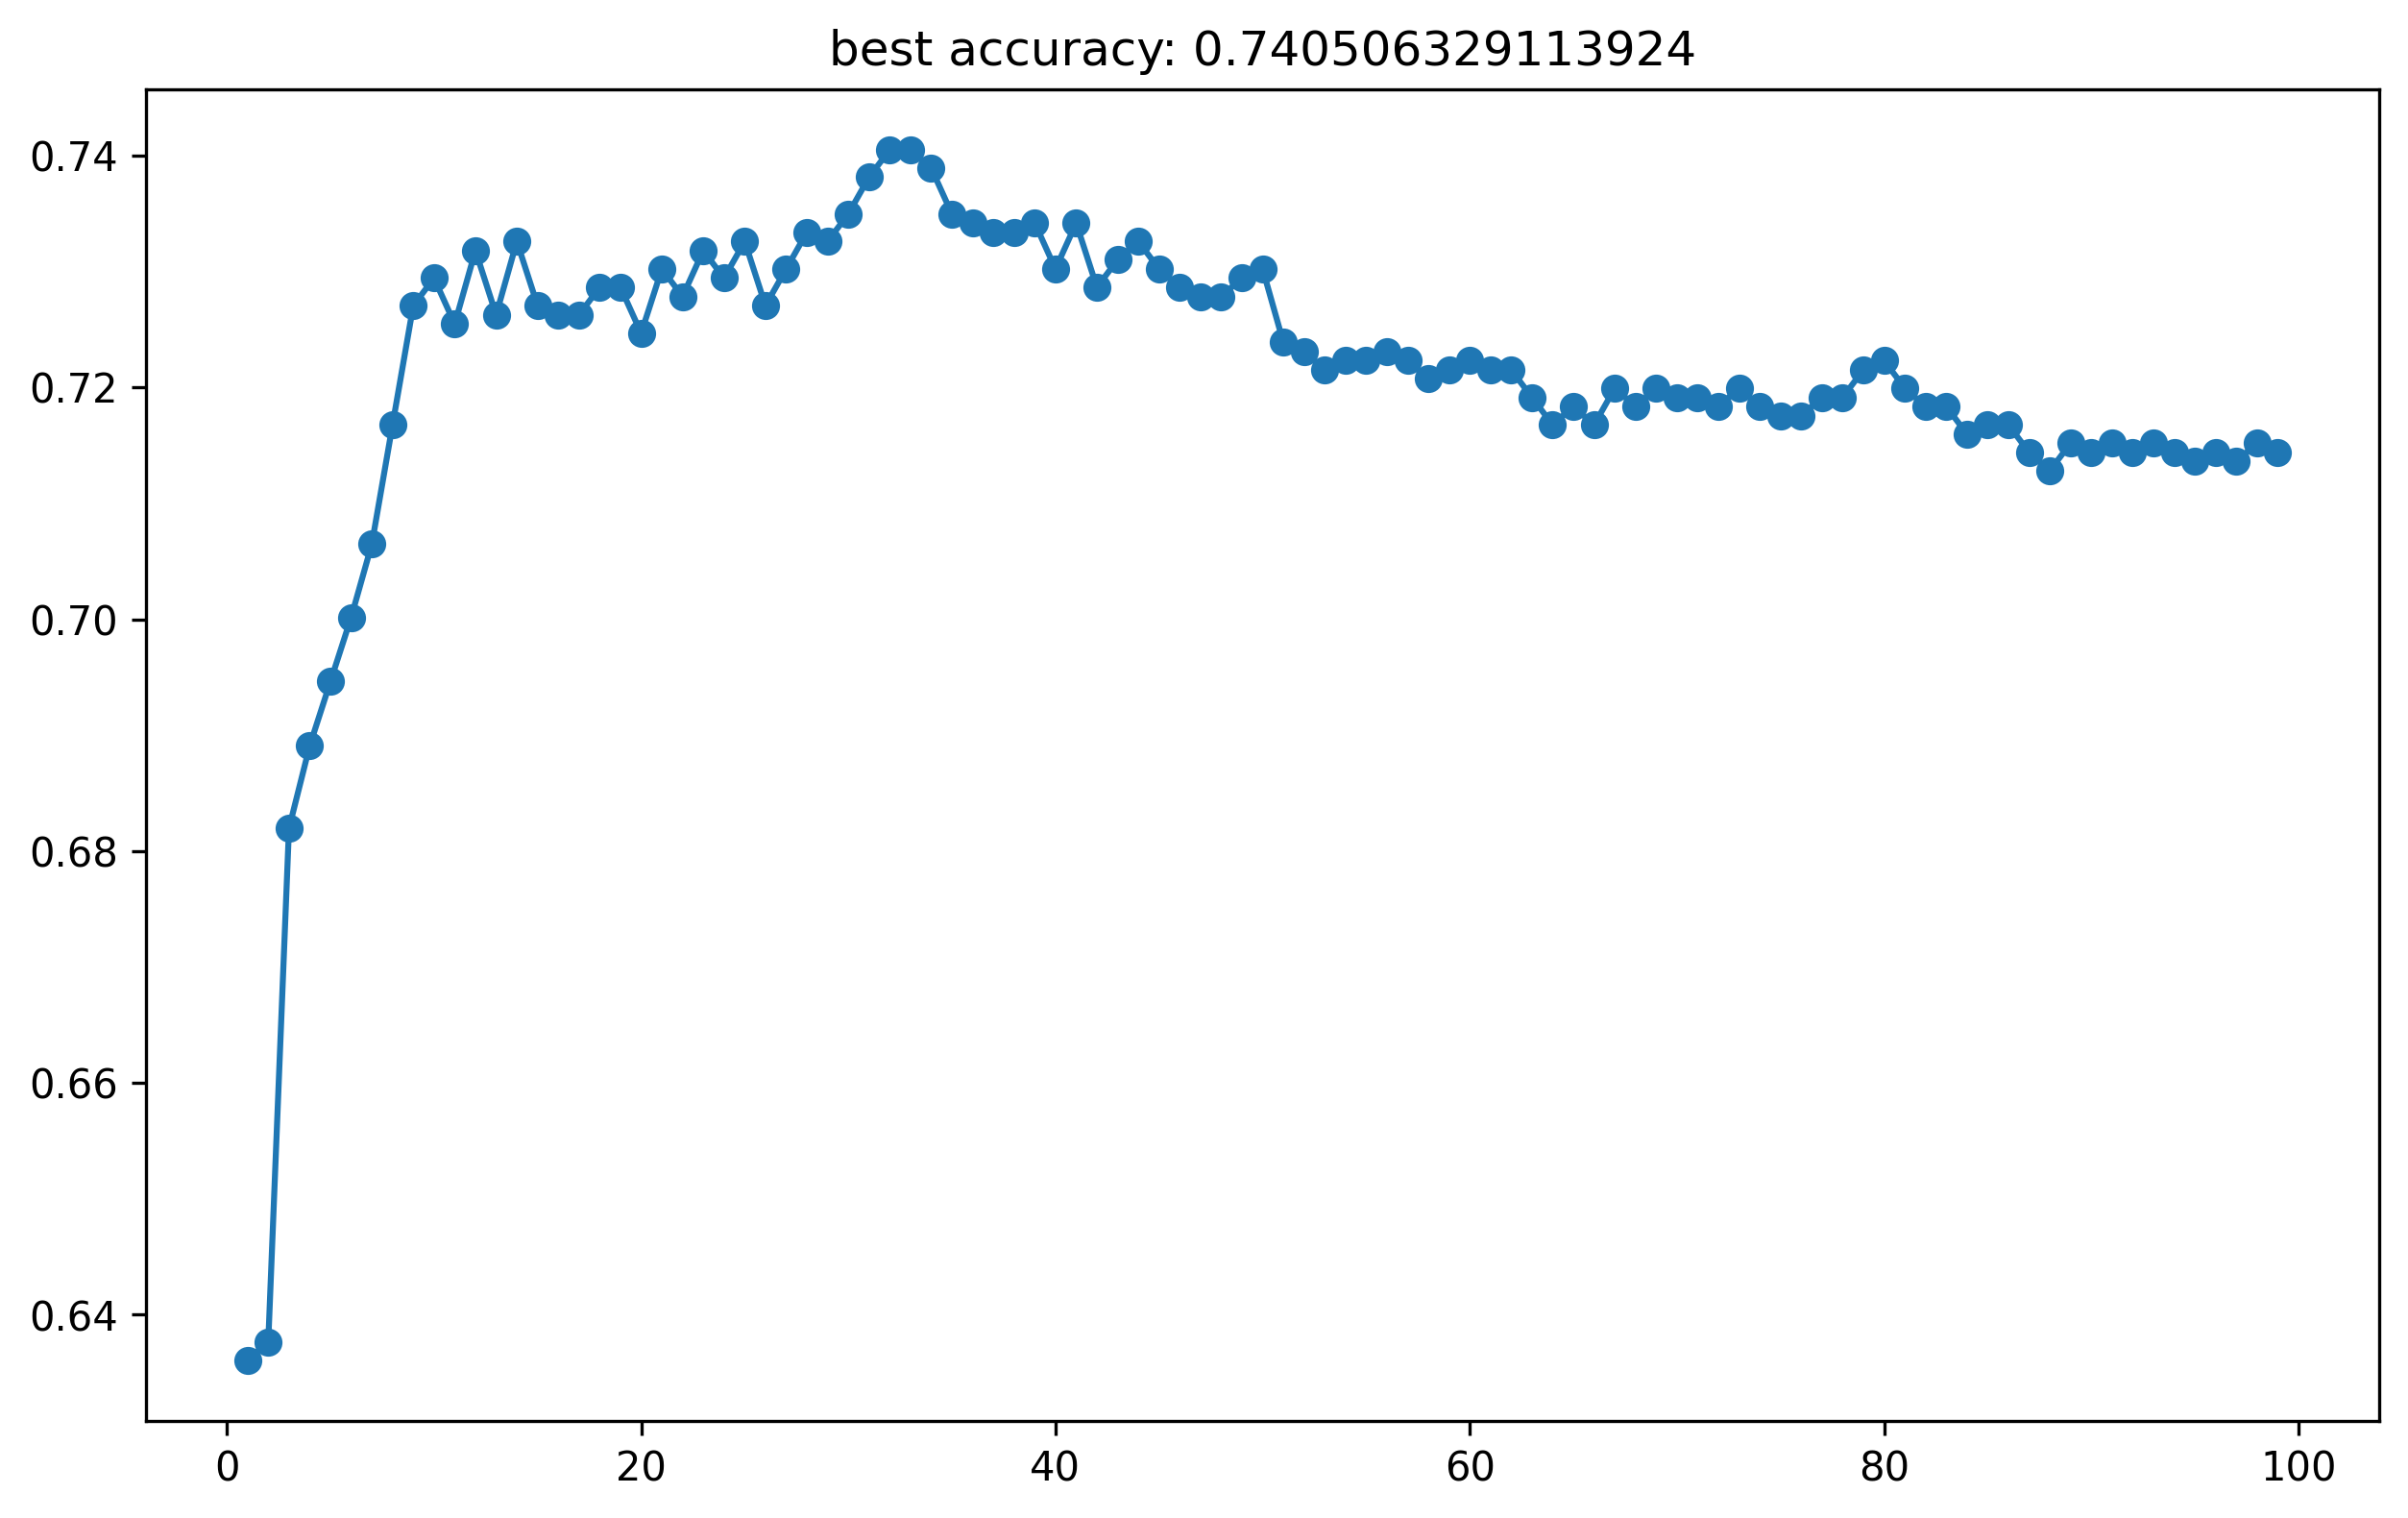
\includegraphics[width=\textwidth]{figures/filtered/knn_acc_7.png}
		\caption*{Accuracy (Filtered): 7×7m}
	\end{minipage}
	\hfill
	\begin{minipage}{0.49\textwidth}
		\centering
		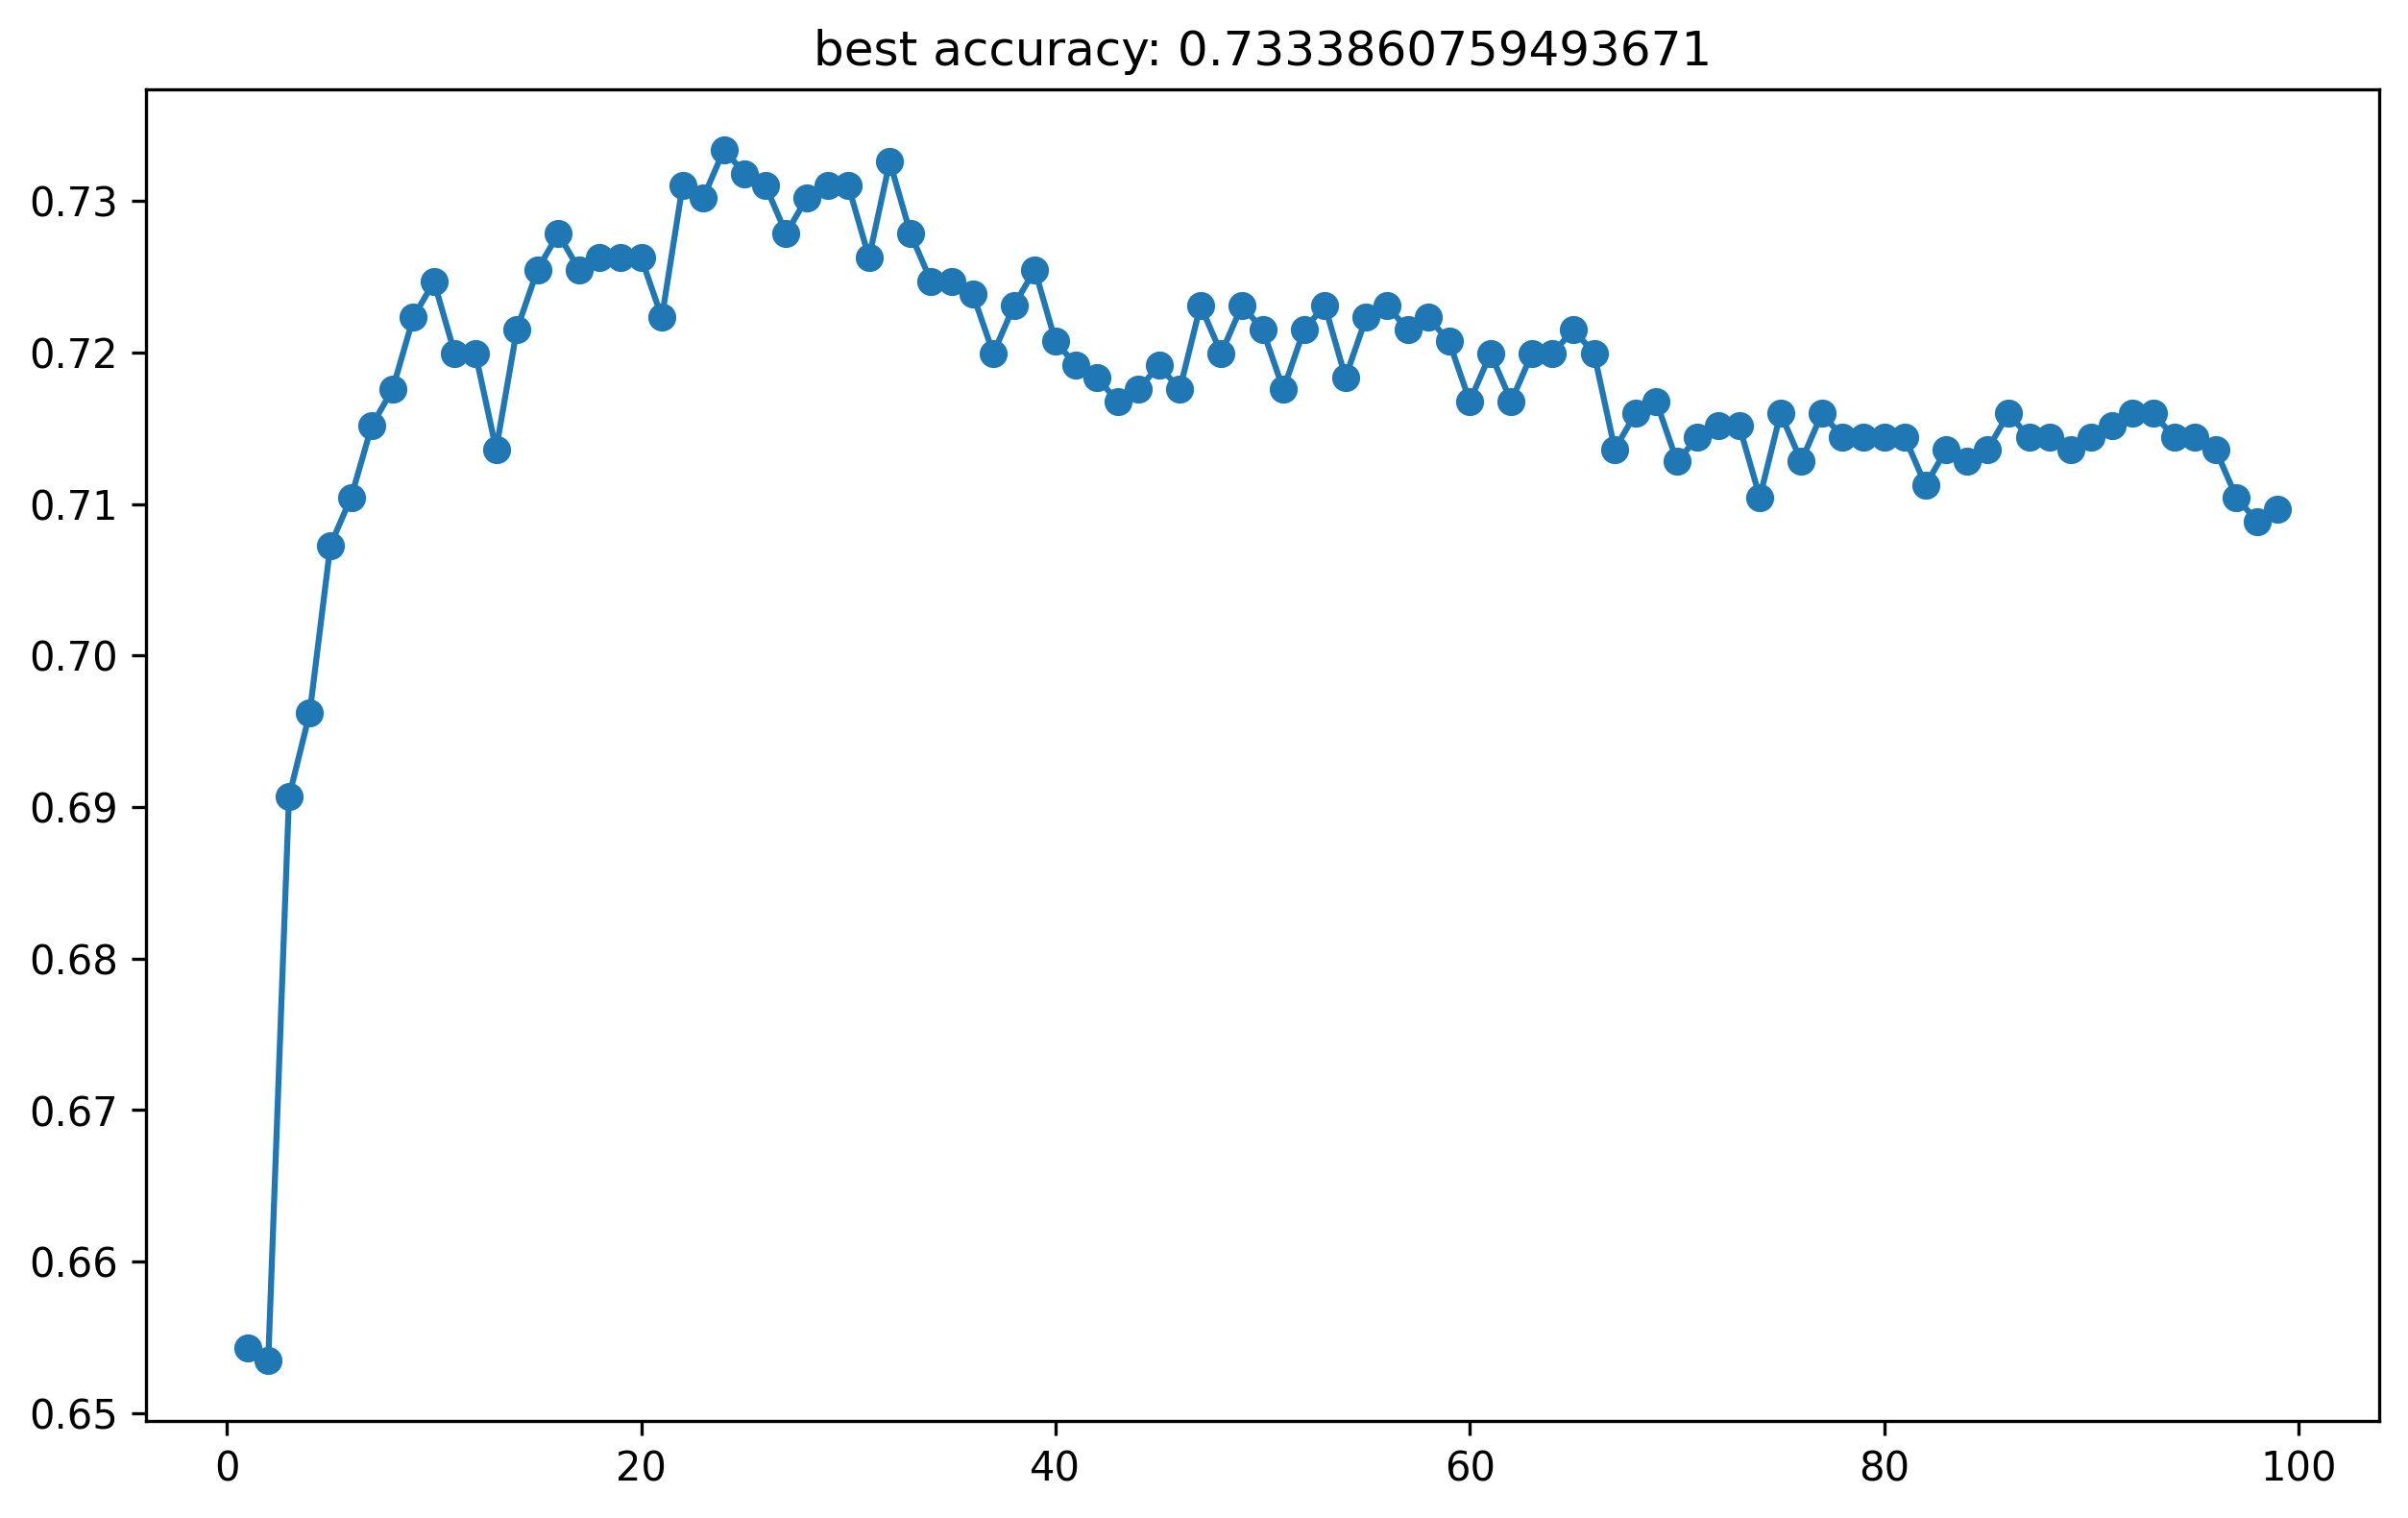
\includegraphics[width=\textwidth]{figures/unfiltered/knn_acc_7.png}
		\caption*{Accuracy (Unfiltered): 7×7m}
	\end{minipage}
\end{figure}

\begin{figure}[H]
	\centering
	\begin{minipage}{0.49\textwidth}
		\centering
		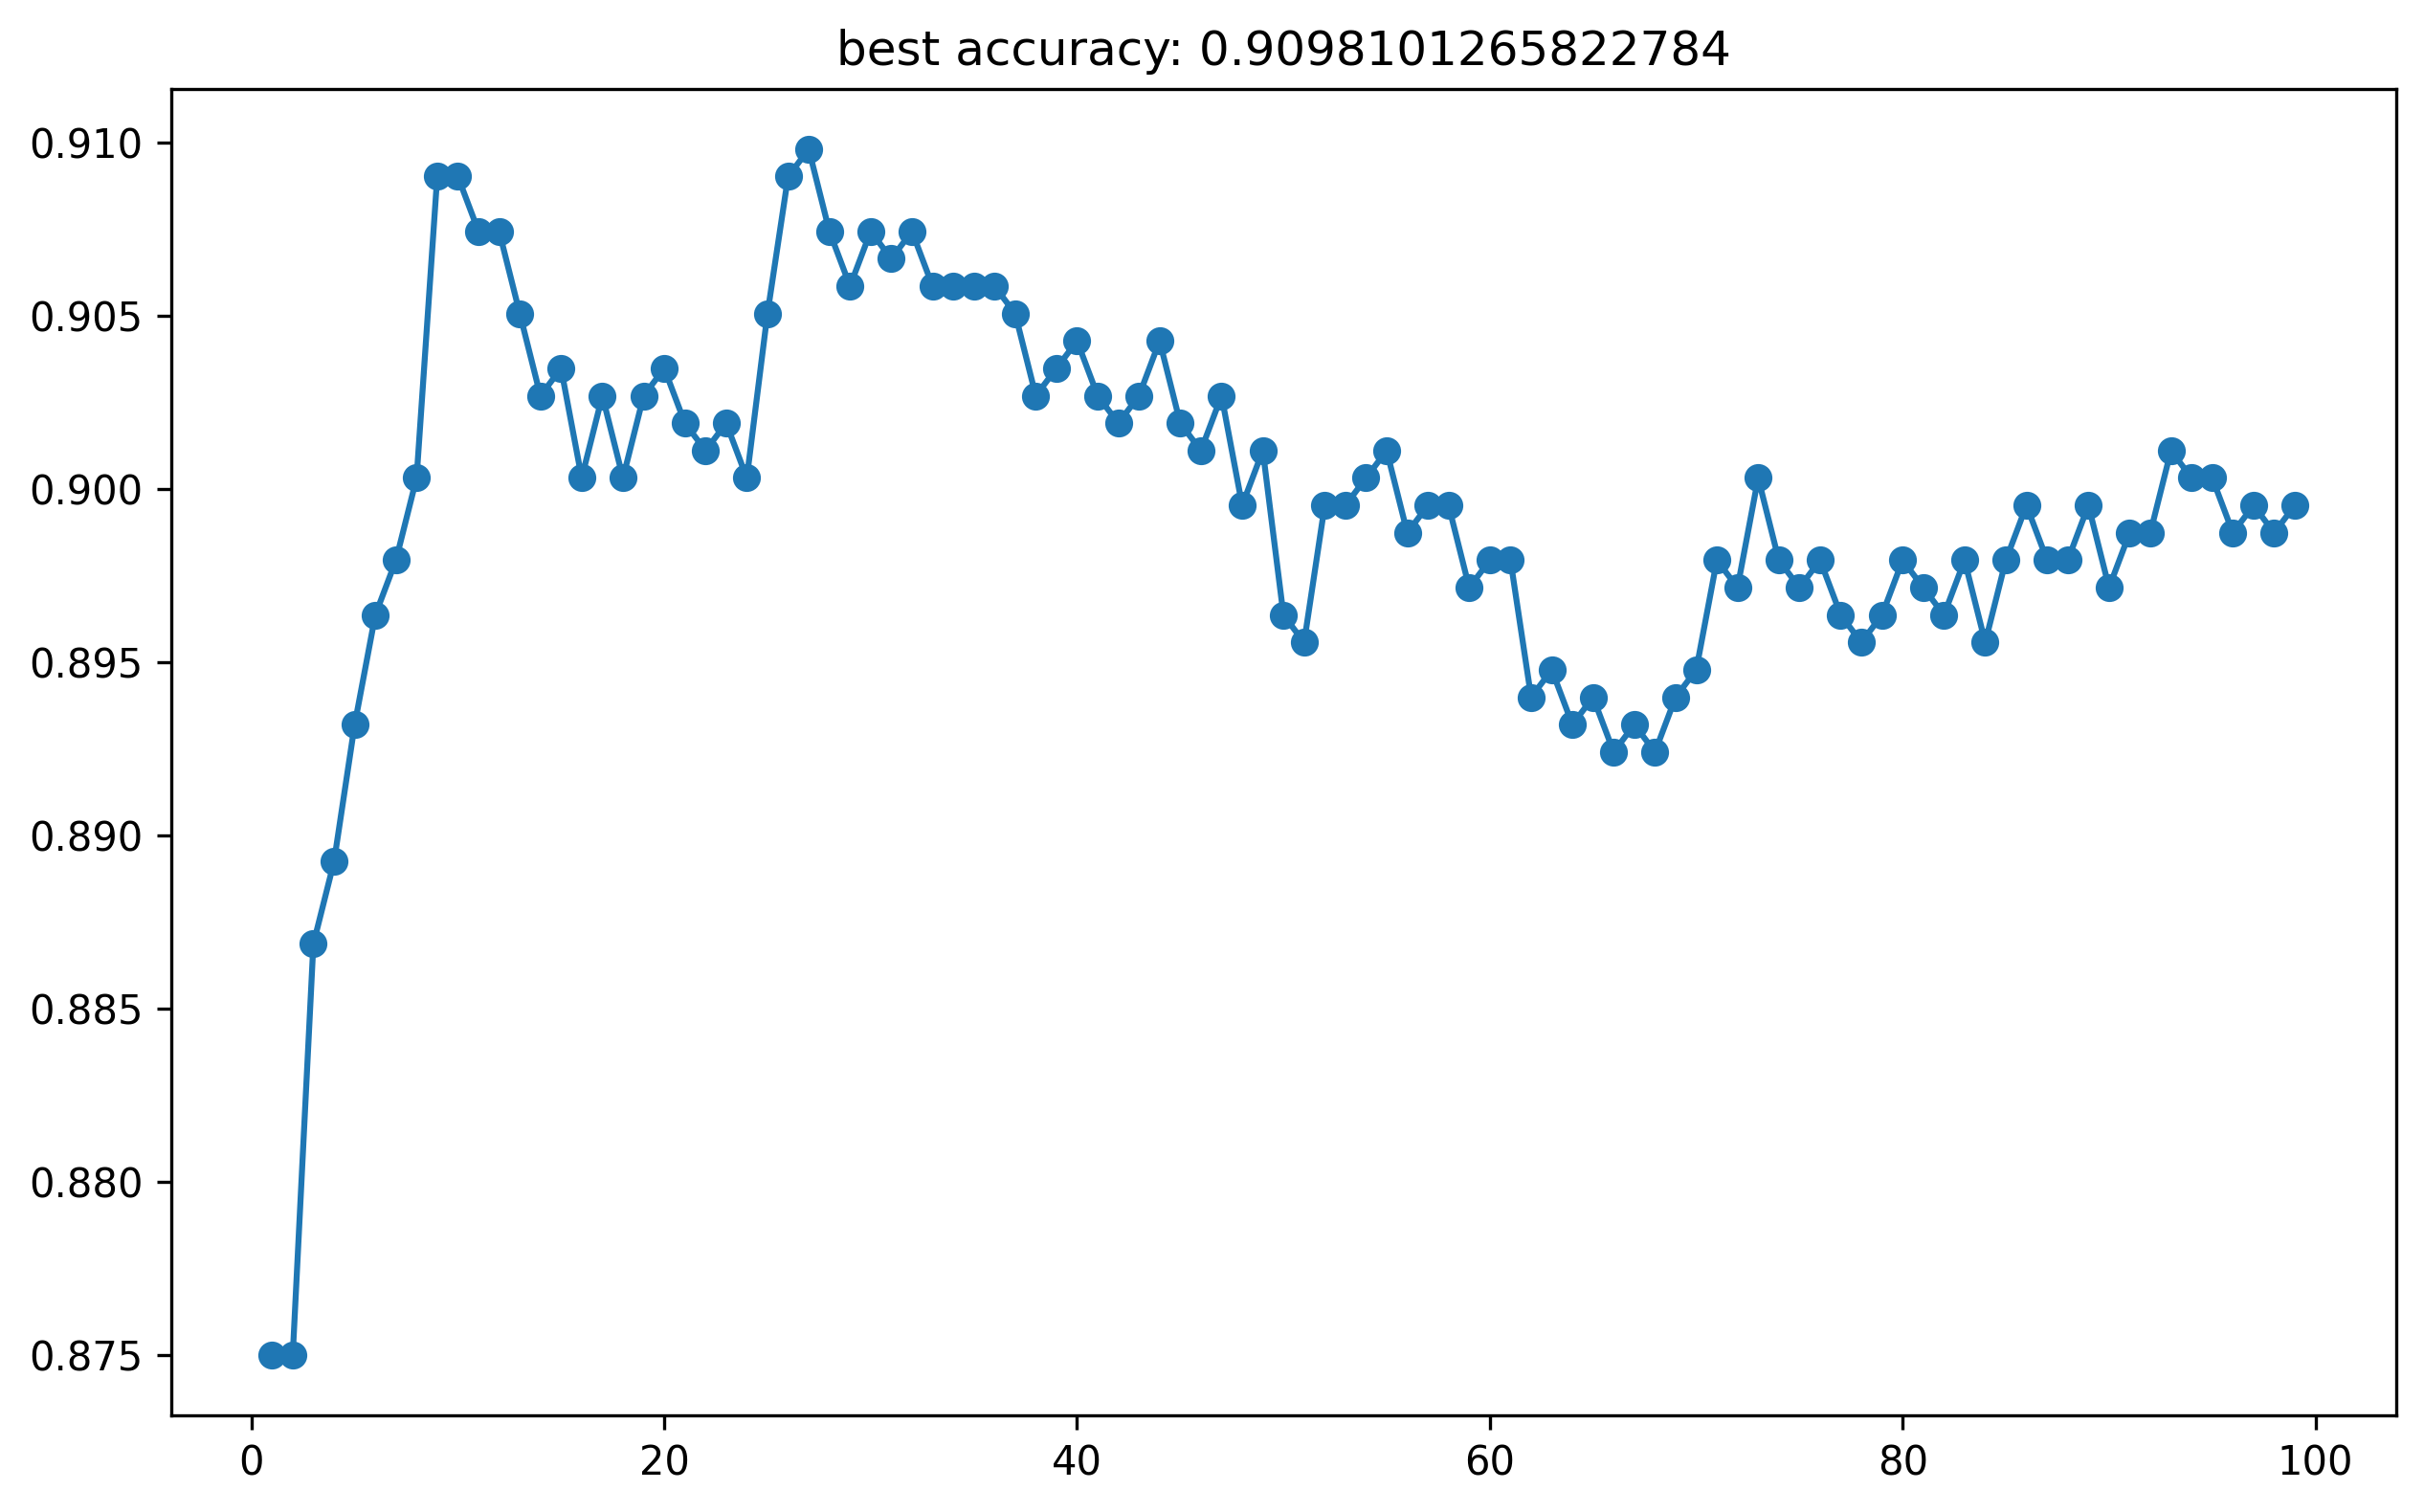
\includegraphics[width=\textwidth]{figures/filtered/knn_acc_15.png}
		\caption*{Accuracy (Filtered): 15×15m}
	\end{minipage}
	\hfill
	\begin{minipage}{0.49\textwidth}
		\centering
		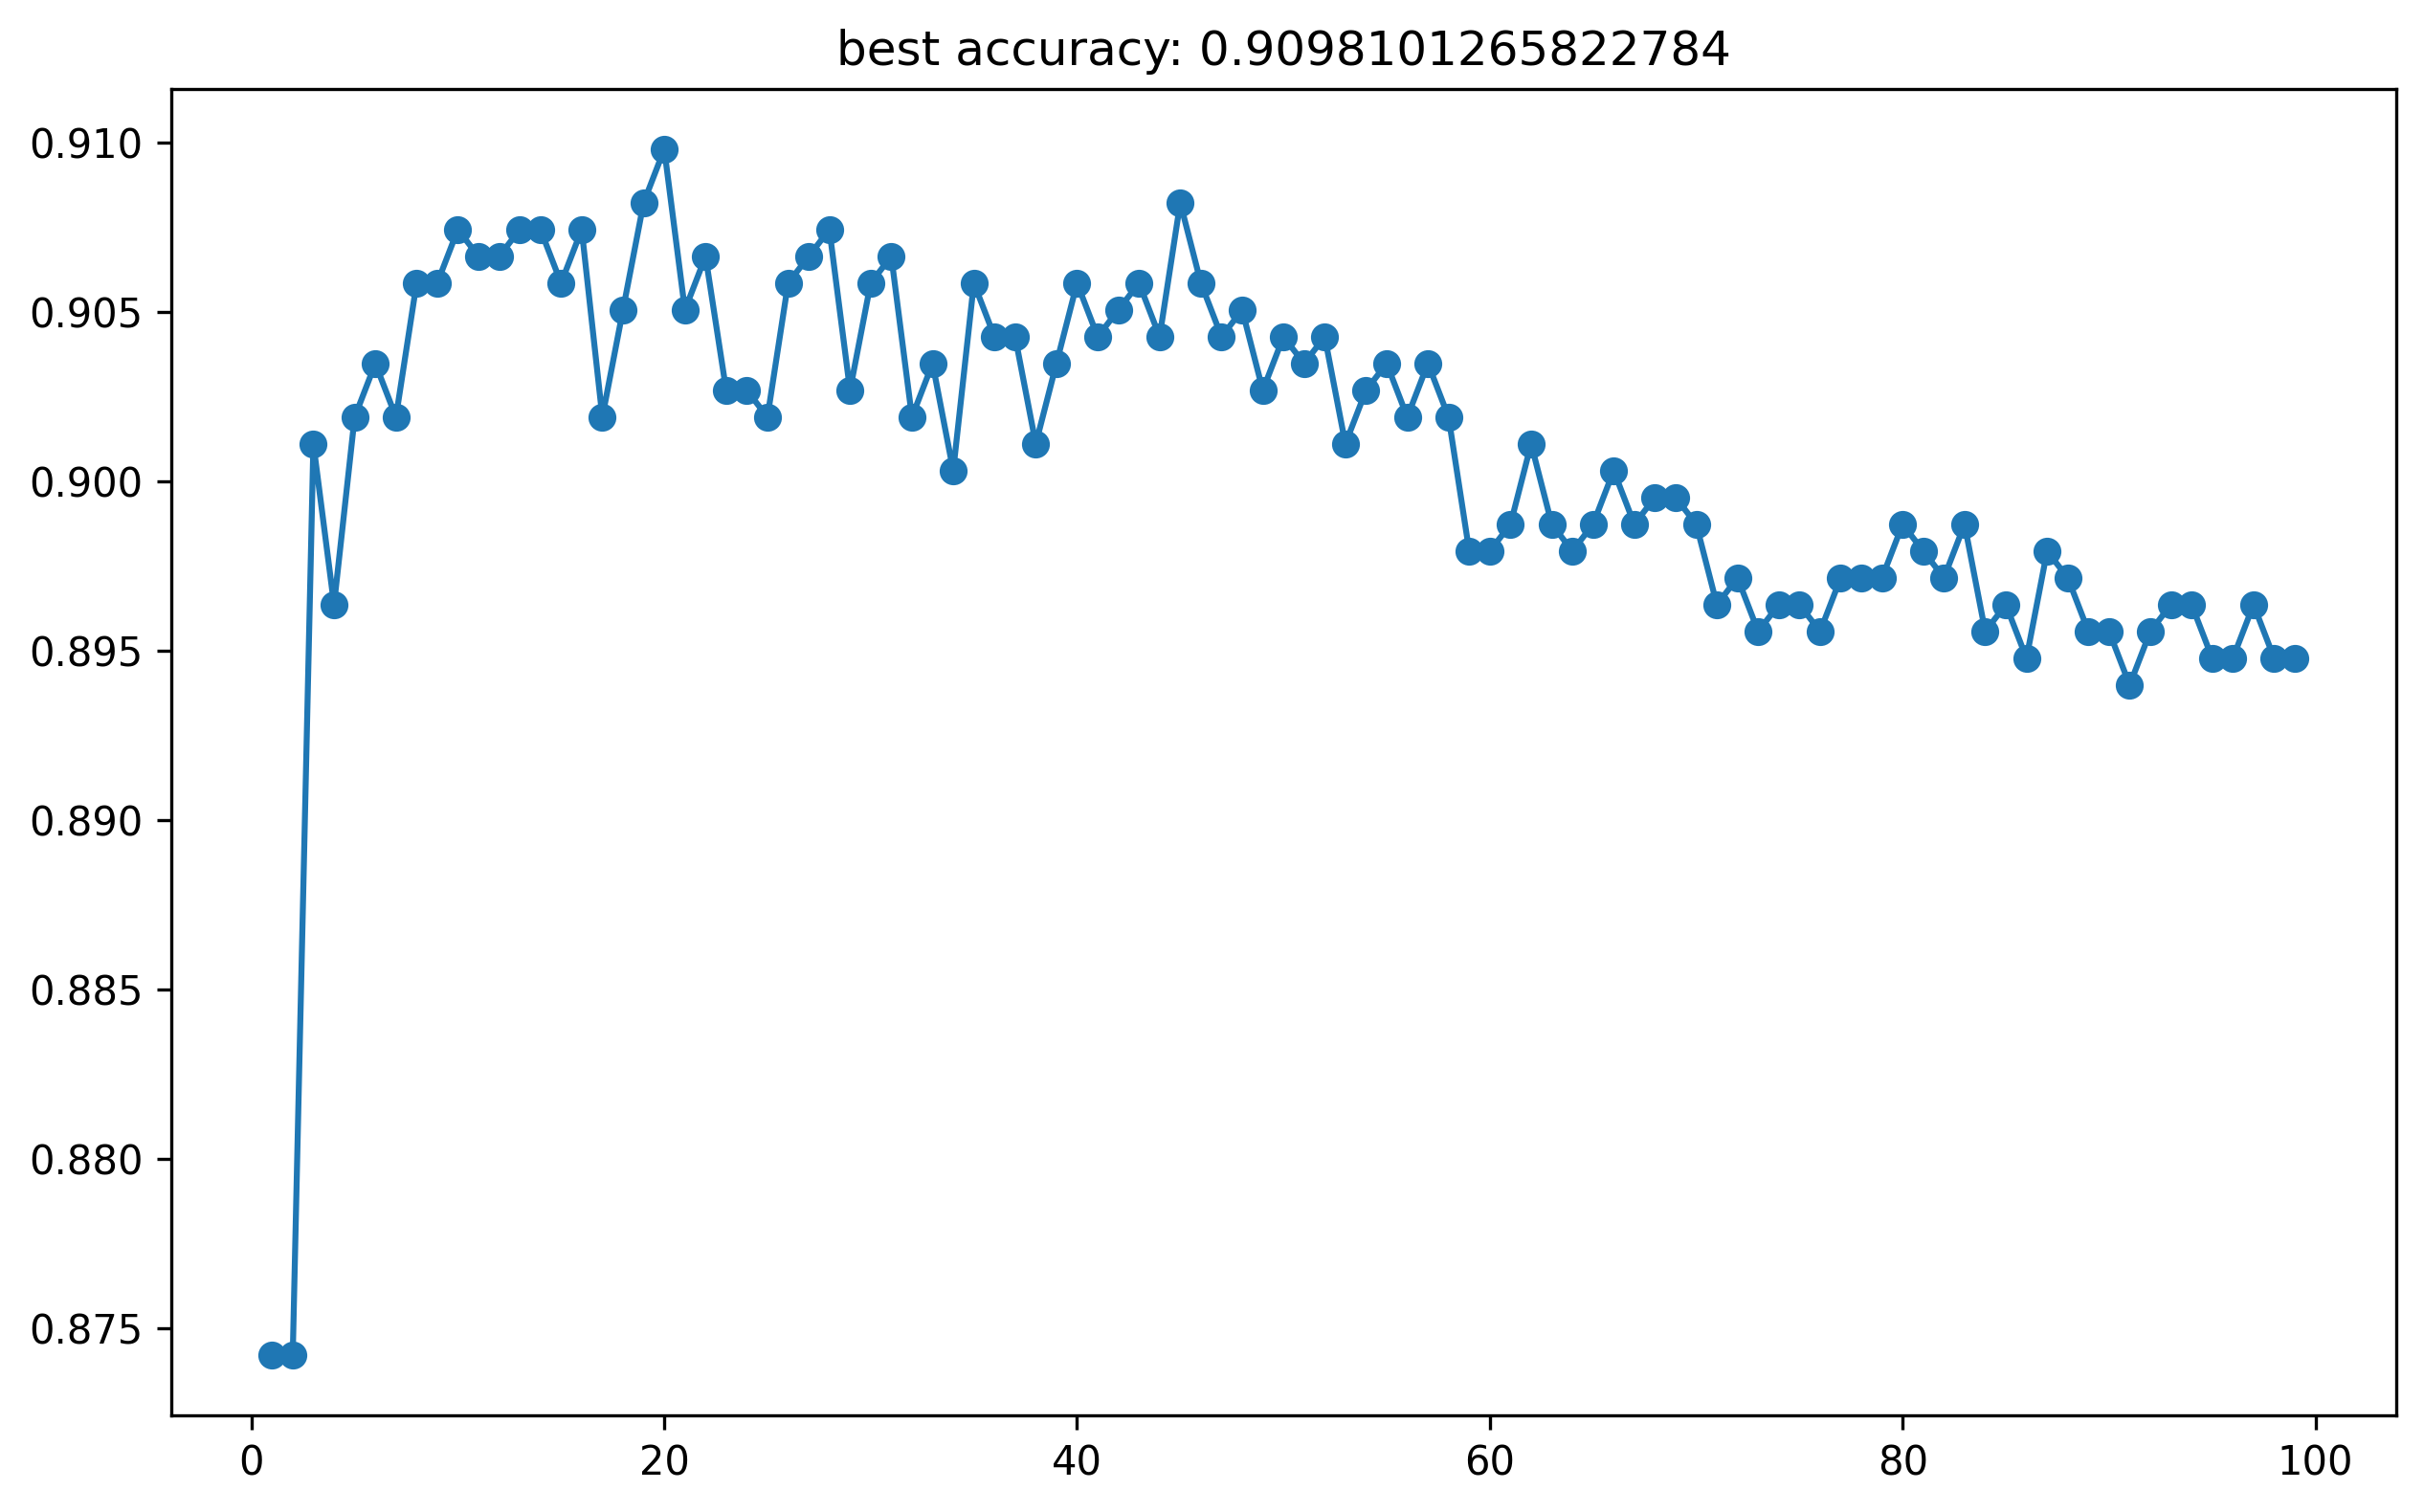
\includegraphics[width=\textwidth]{figures/unfiltered/knn_acc_15.png}
		\caption*{Accuracy (Unfiltered): 15×15m}
	\end{minipage}
\end{figure}

\begin{figure}[H]
	\centering
	\begin{minipage}{0.49\textwidth}
		\centering
		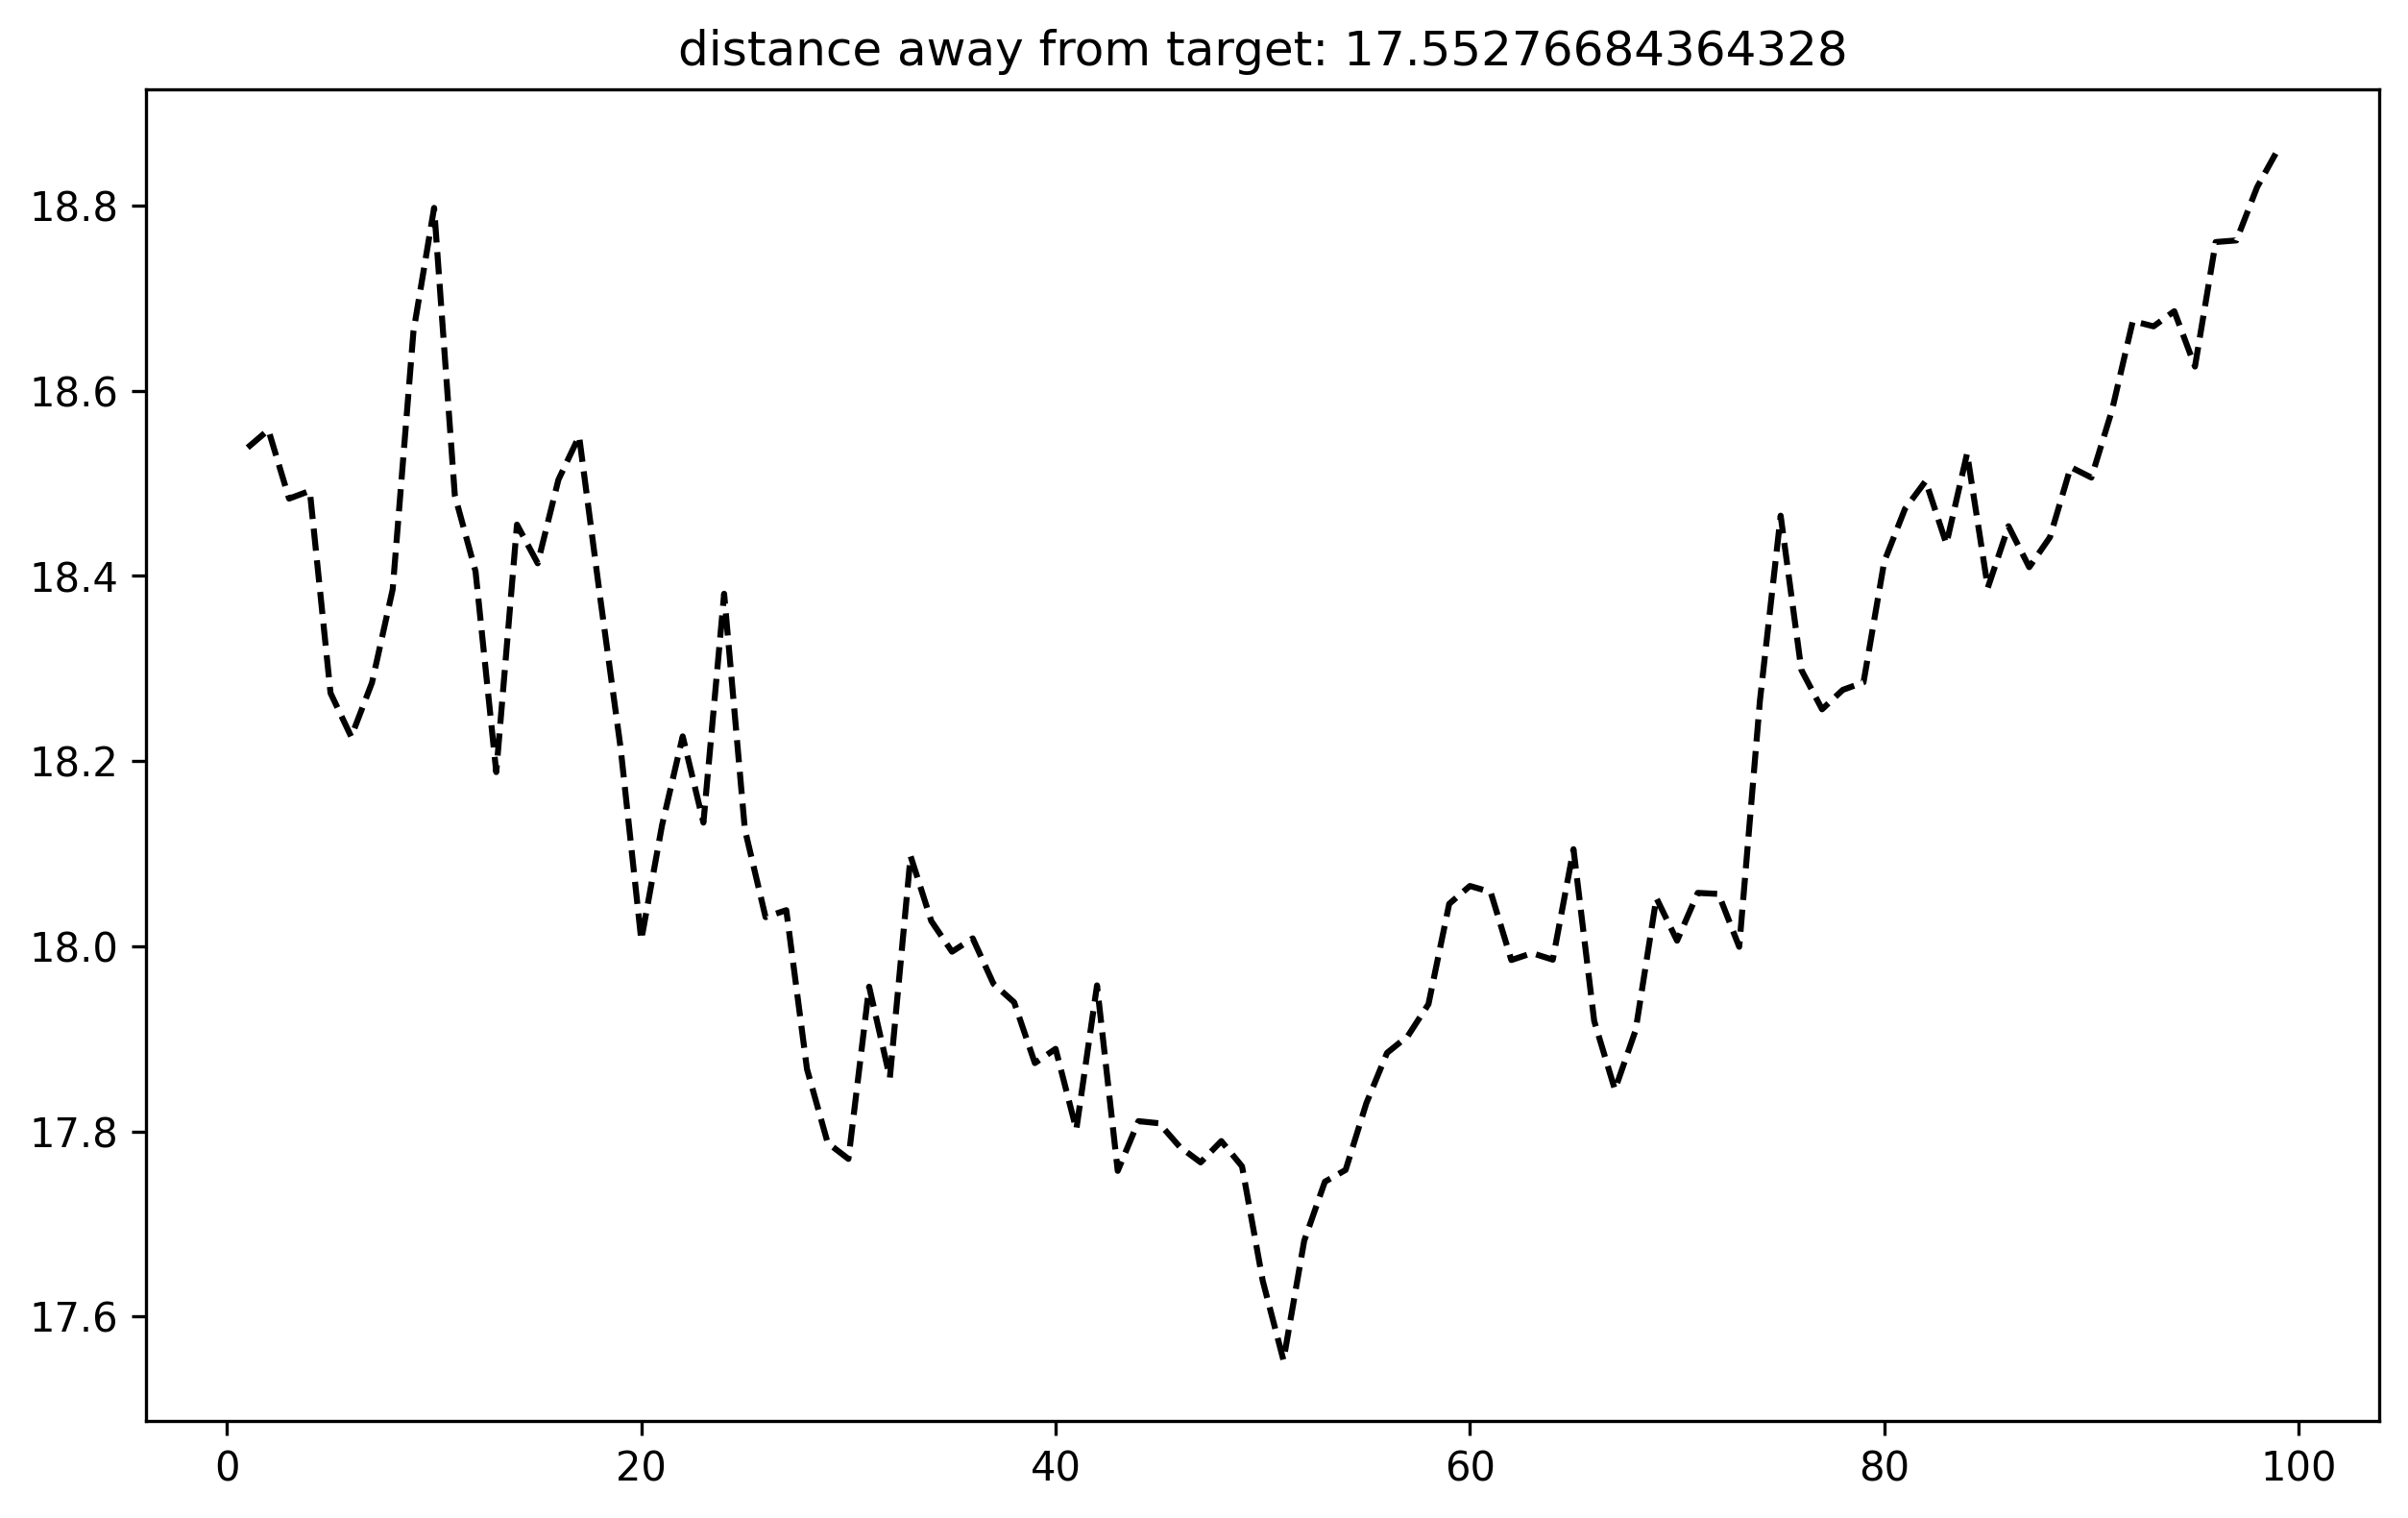
\includegraphics[width=\textwidth]{figures/filtered/knn_custom_1.png}
		\caption*{AGT (Filtered): 1×1m}
	\end{minipage}
	\hfill
	\begin{minipage}{0.49\textwidth}
		\centering
		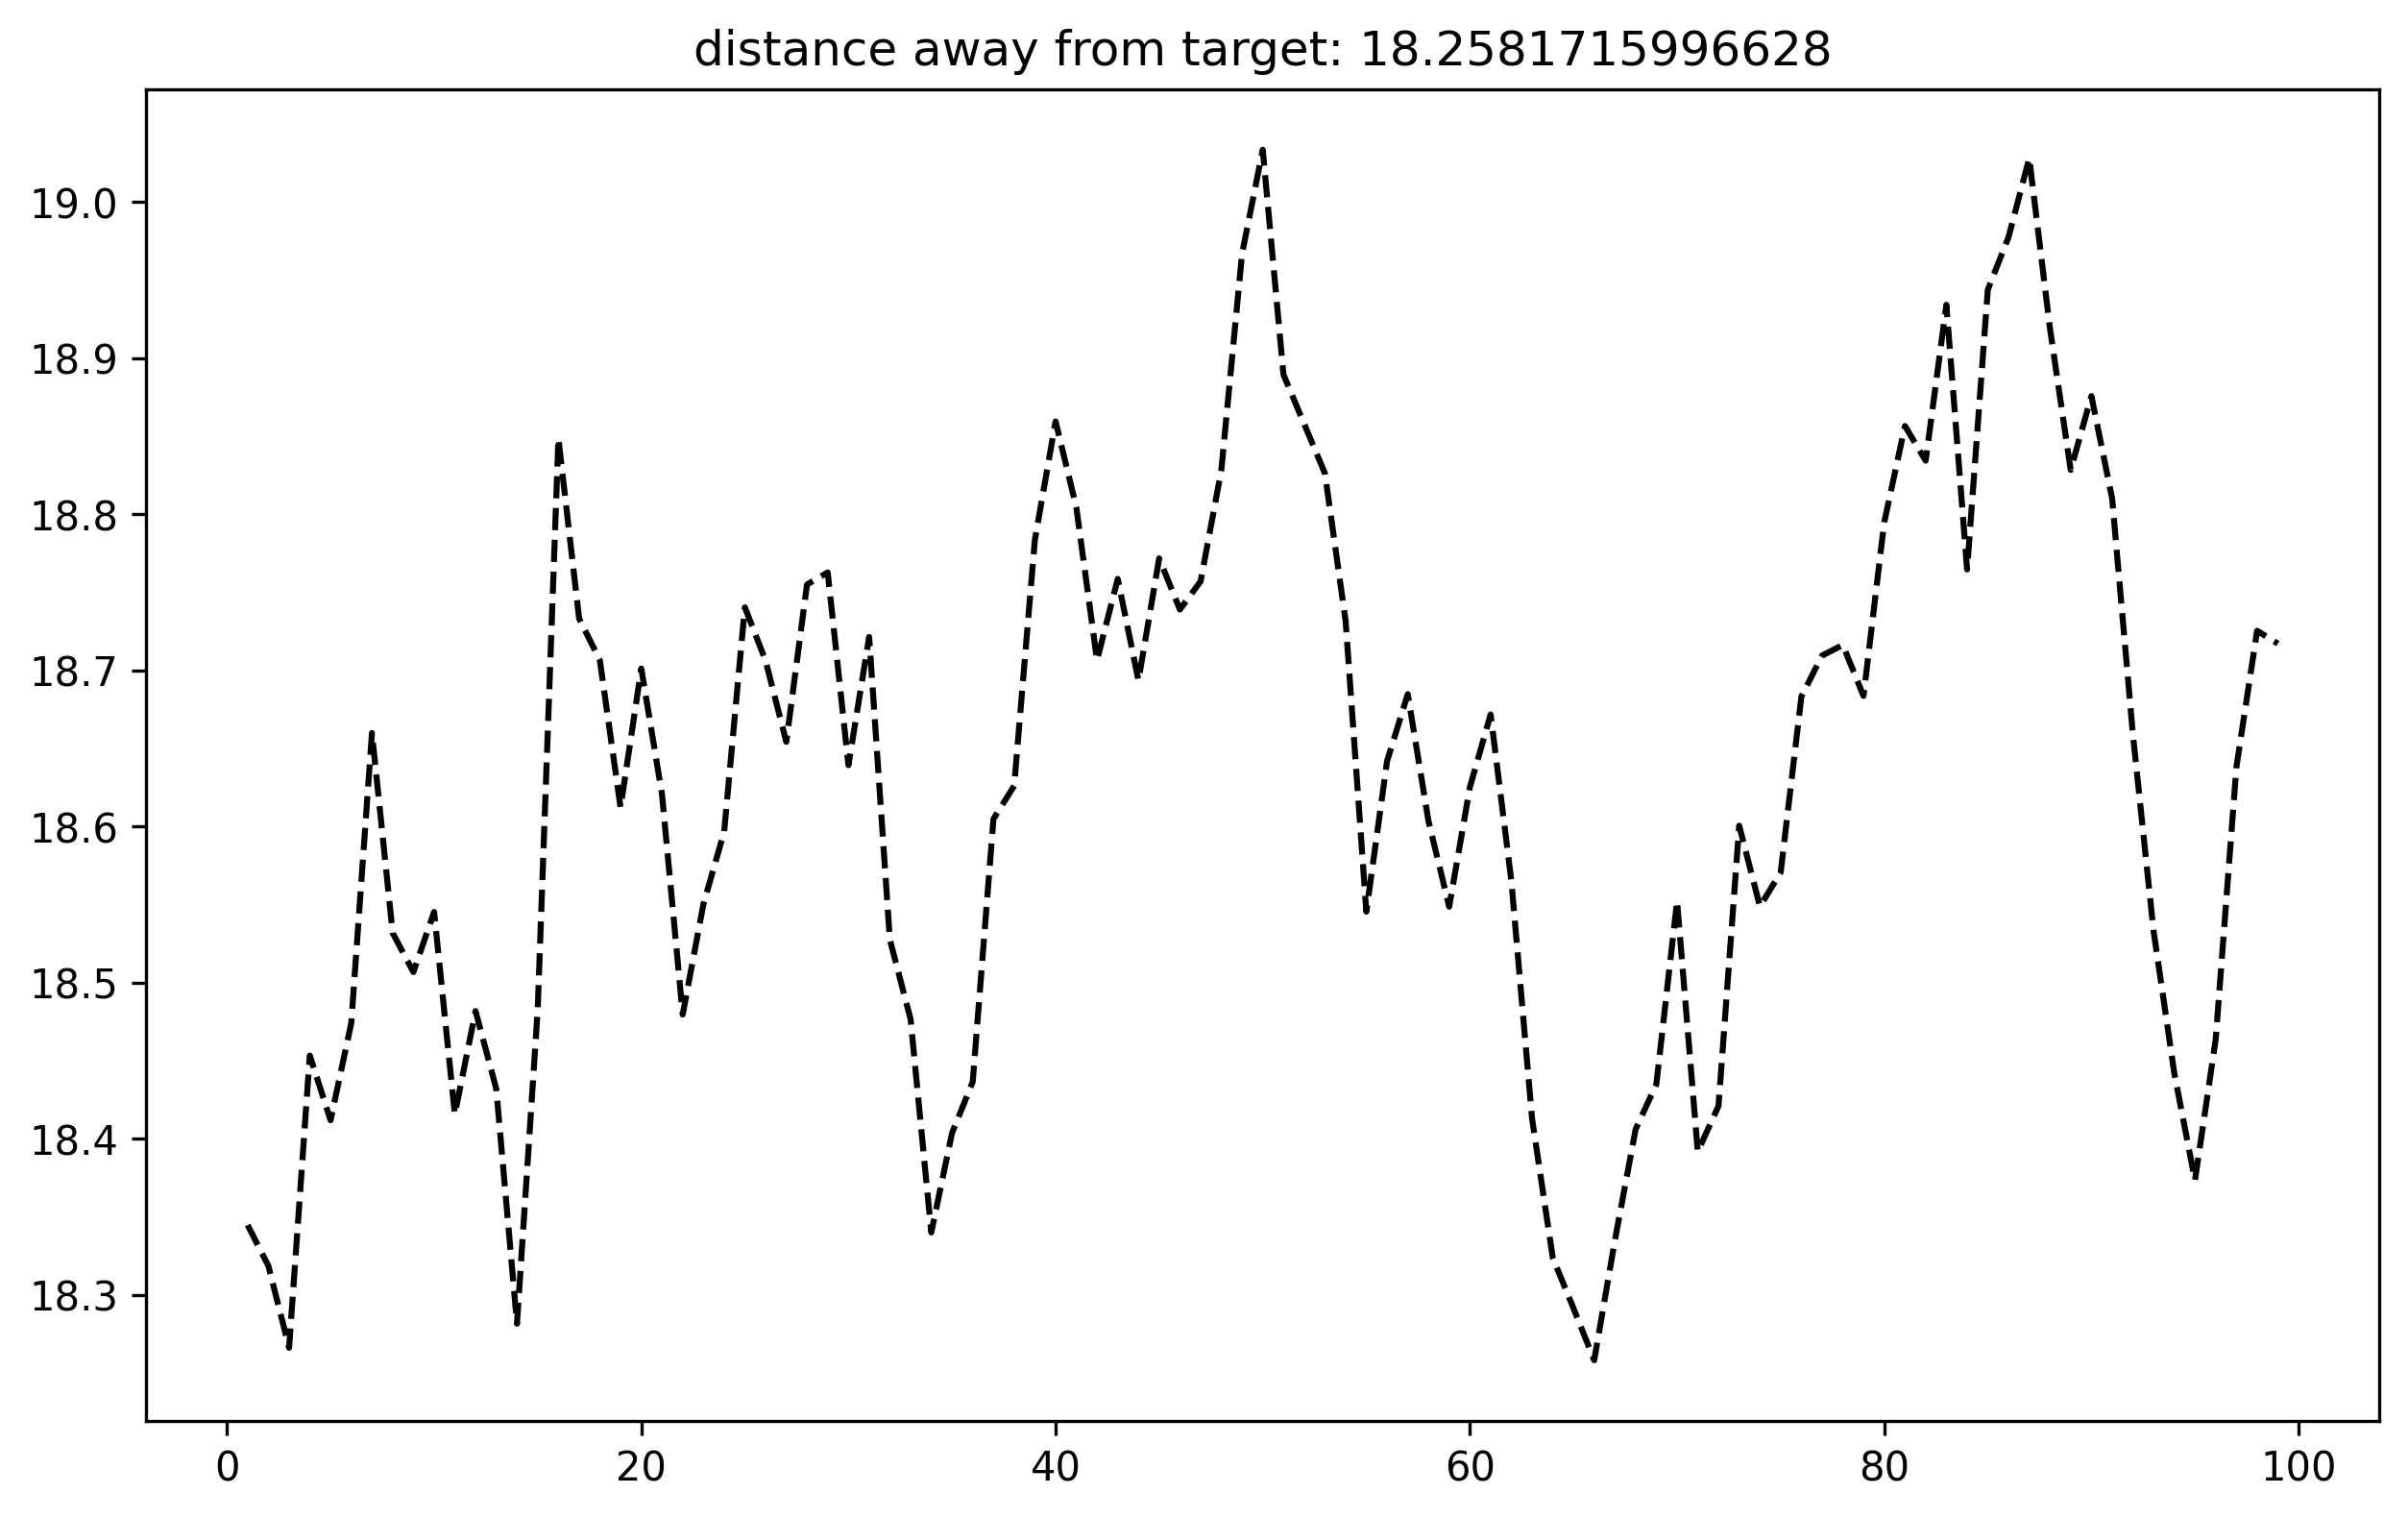
\includegraphics[width=\textwidth]{figures/unfiltered/knn_custom_1.png}
		\caption*{AGT (Unfiltered): 1×1m}
	\end{minipage}
\end{figure}

\begin{figure}[H]
	\centering
	\begin{minipage}{0.49\textwidth}
		\centering
		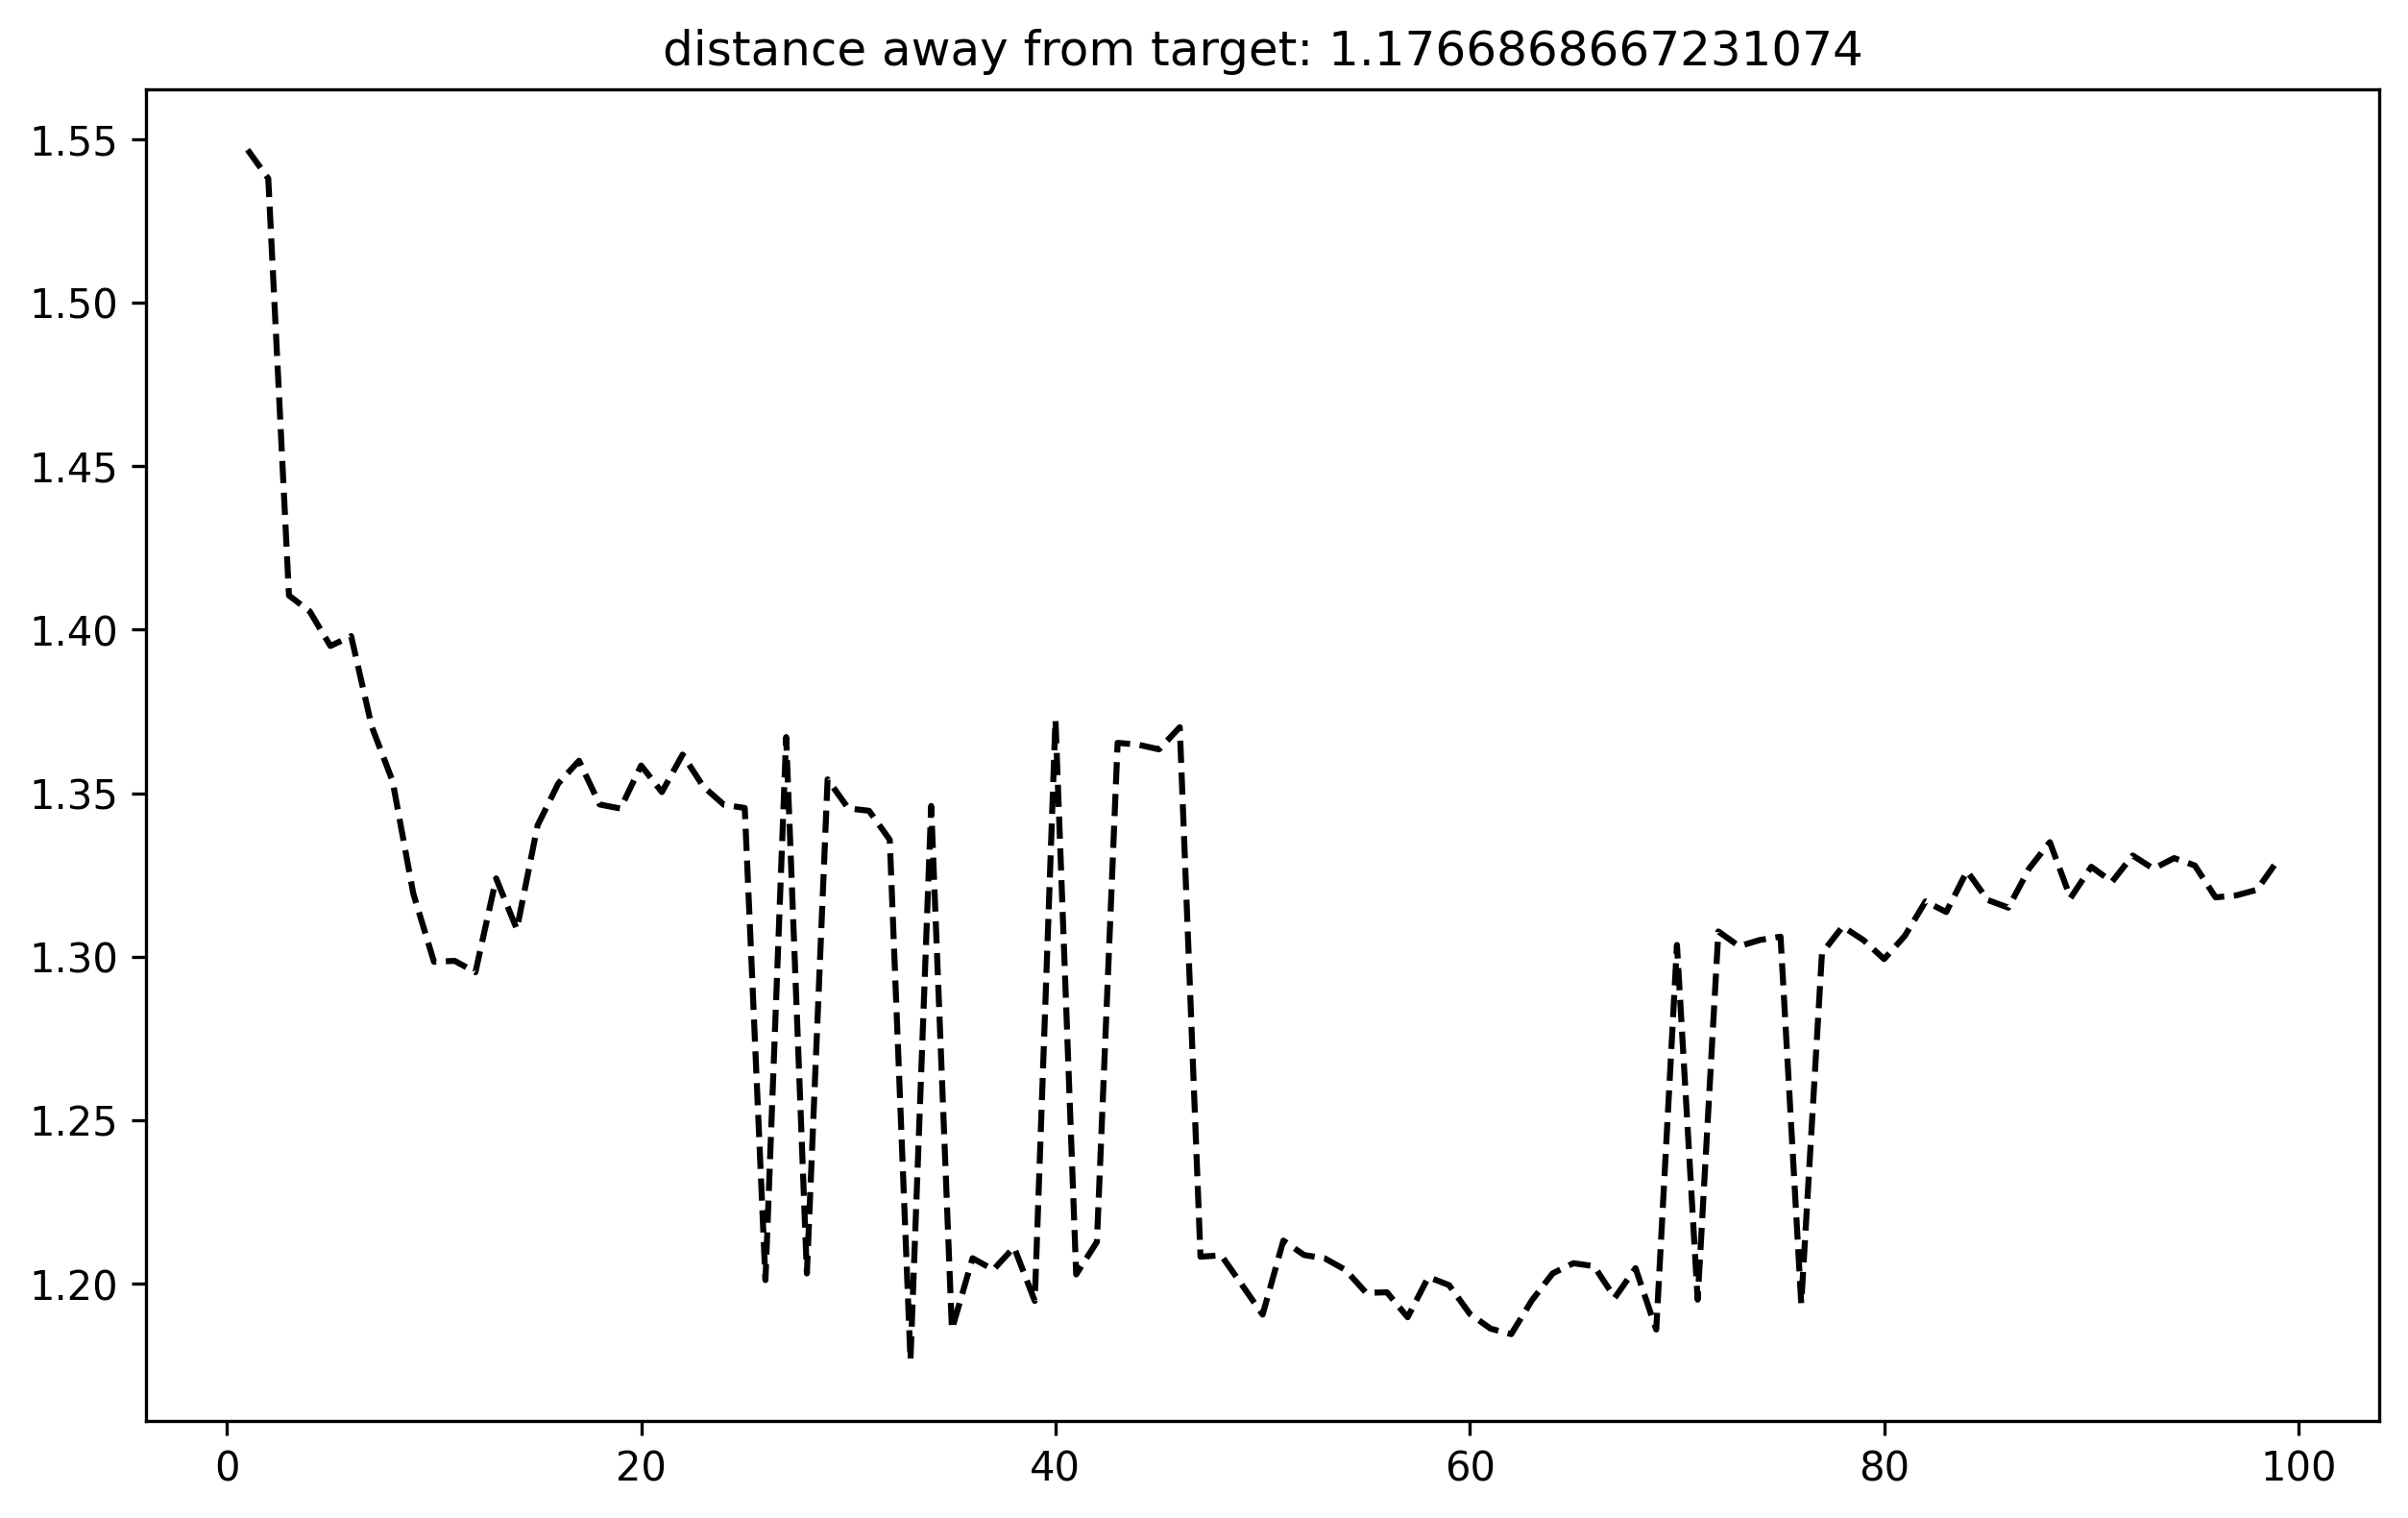
\includegraphics[width=\textwidth]{figures/filtered/knn_custom_7.png}
		\caption*{AGT (Filtered): 7×7m}
	\end{minipage}
	\hfill
	\begin{minipage}{0.49\textwidth}
		\centering
		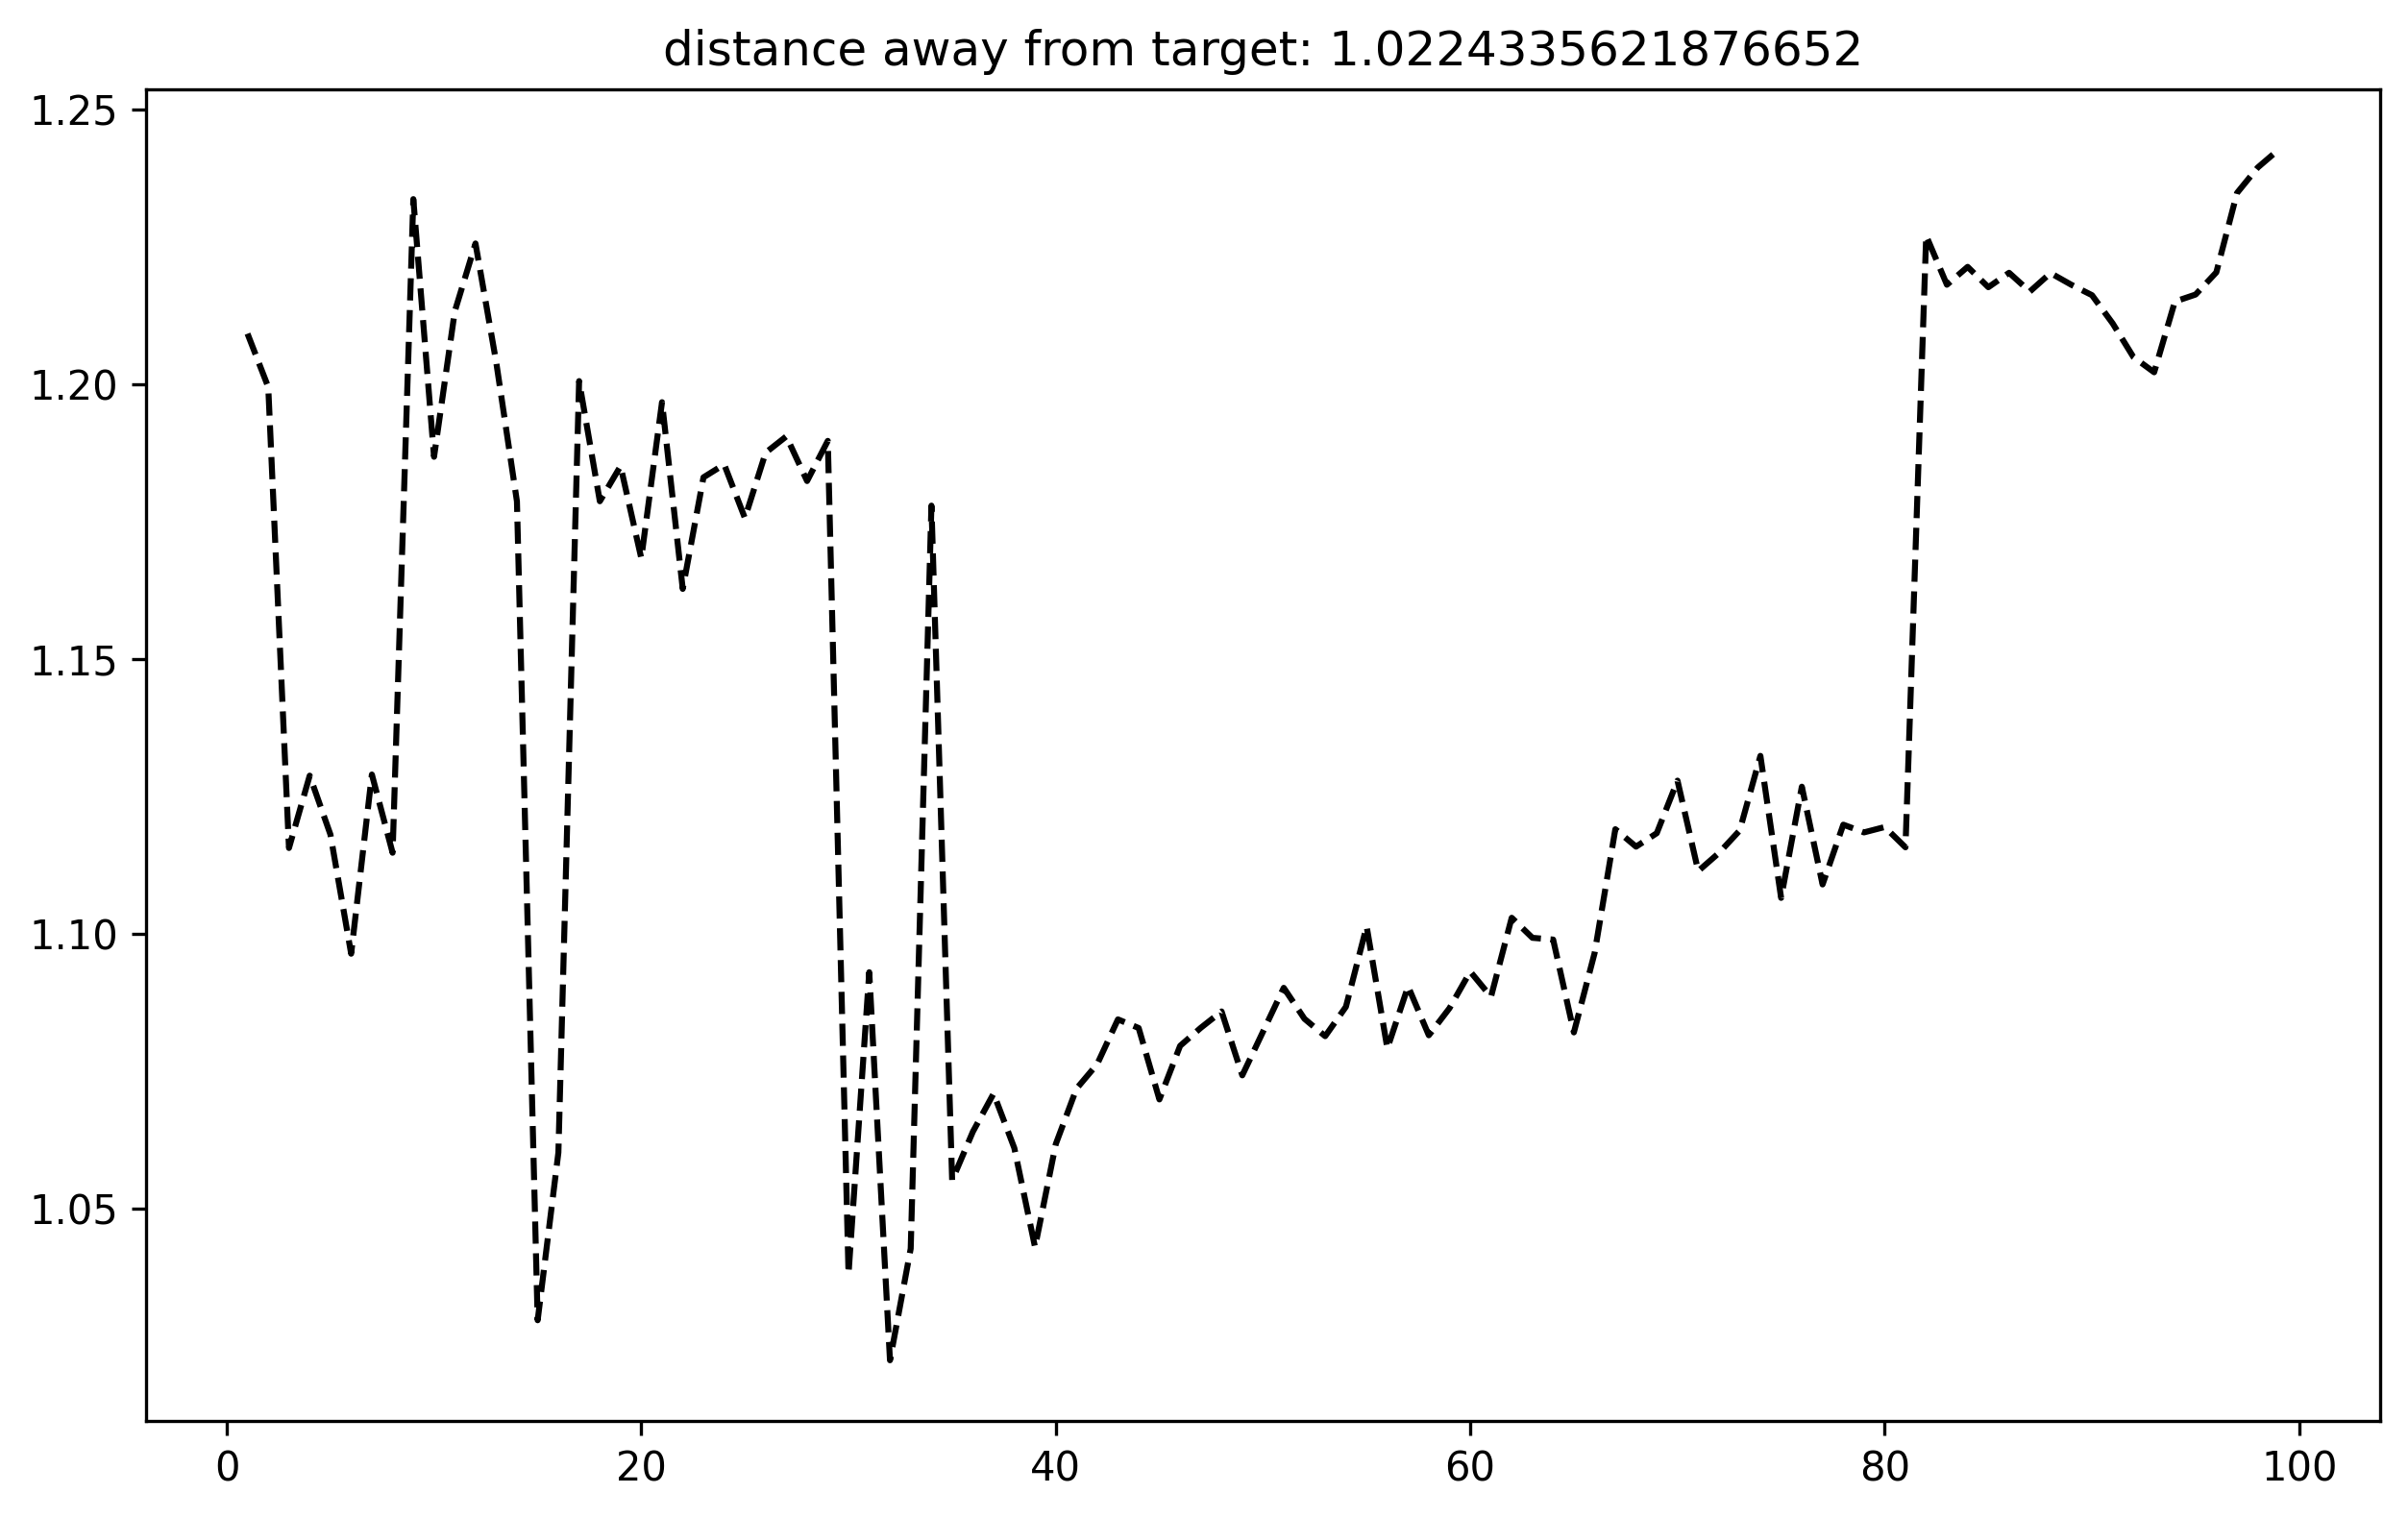
\includegraphics[width=\textwidth]{figures/unfiltered/knn_custom_7.png}
		\caption*{AGT (Unfiltered): 7×7m}
	\end{minipage}
\end{figure}

\begin{figure}[H]
	\centering
	\begin{minipage}{0.49\textwidth}
		\centering
		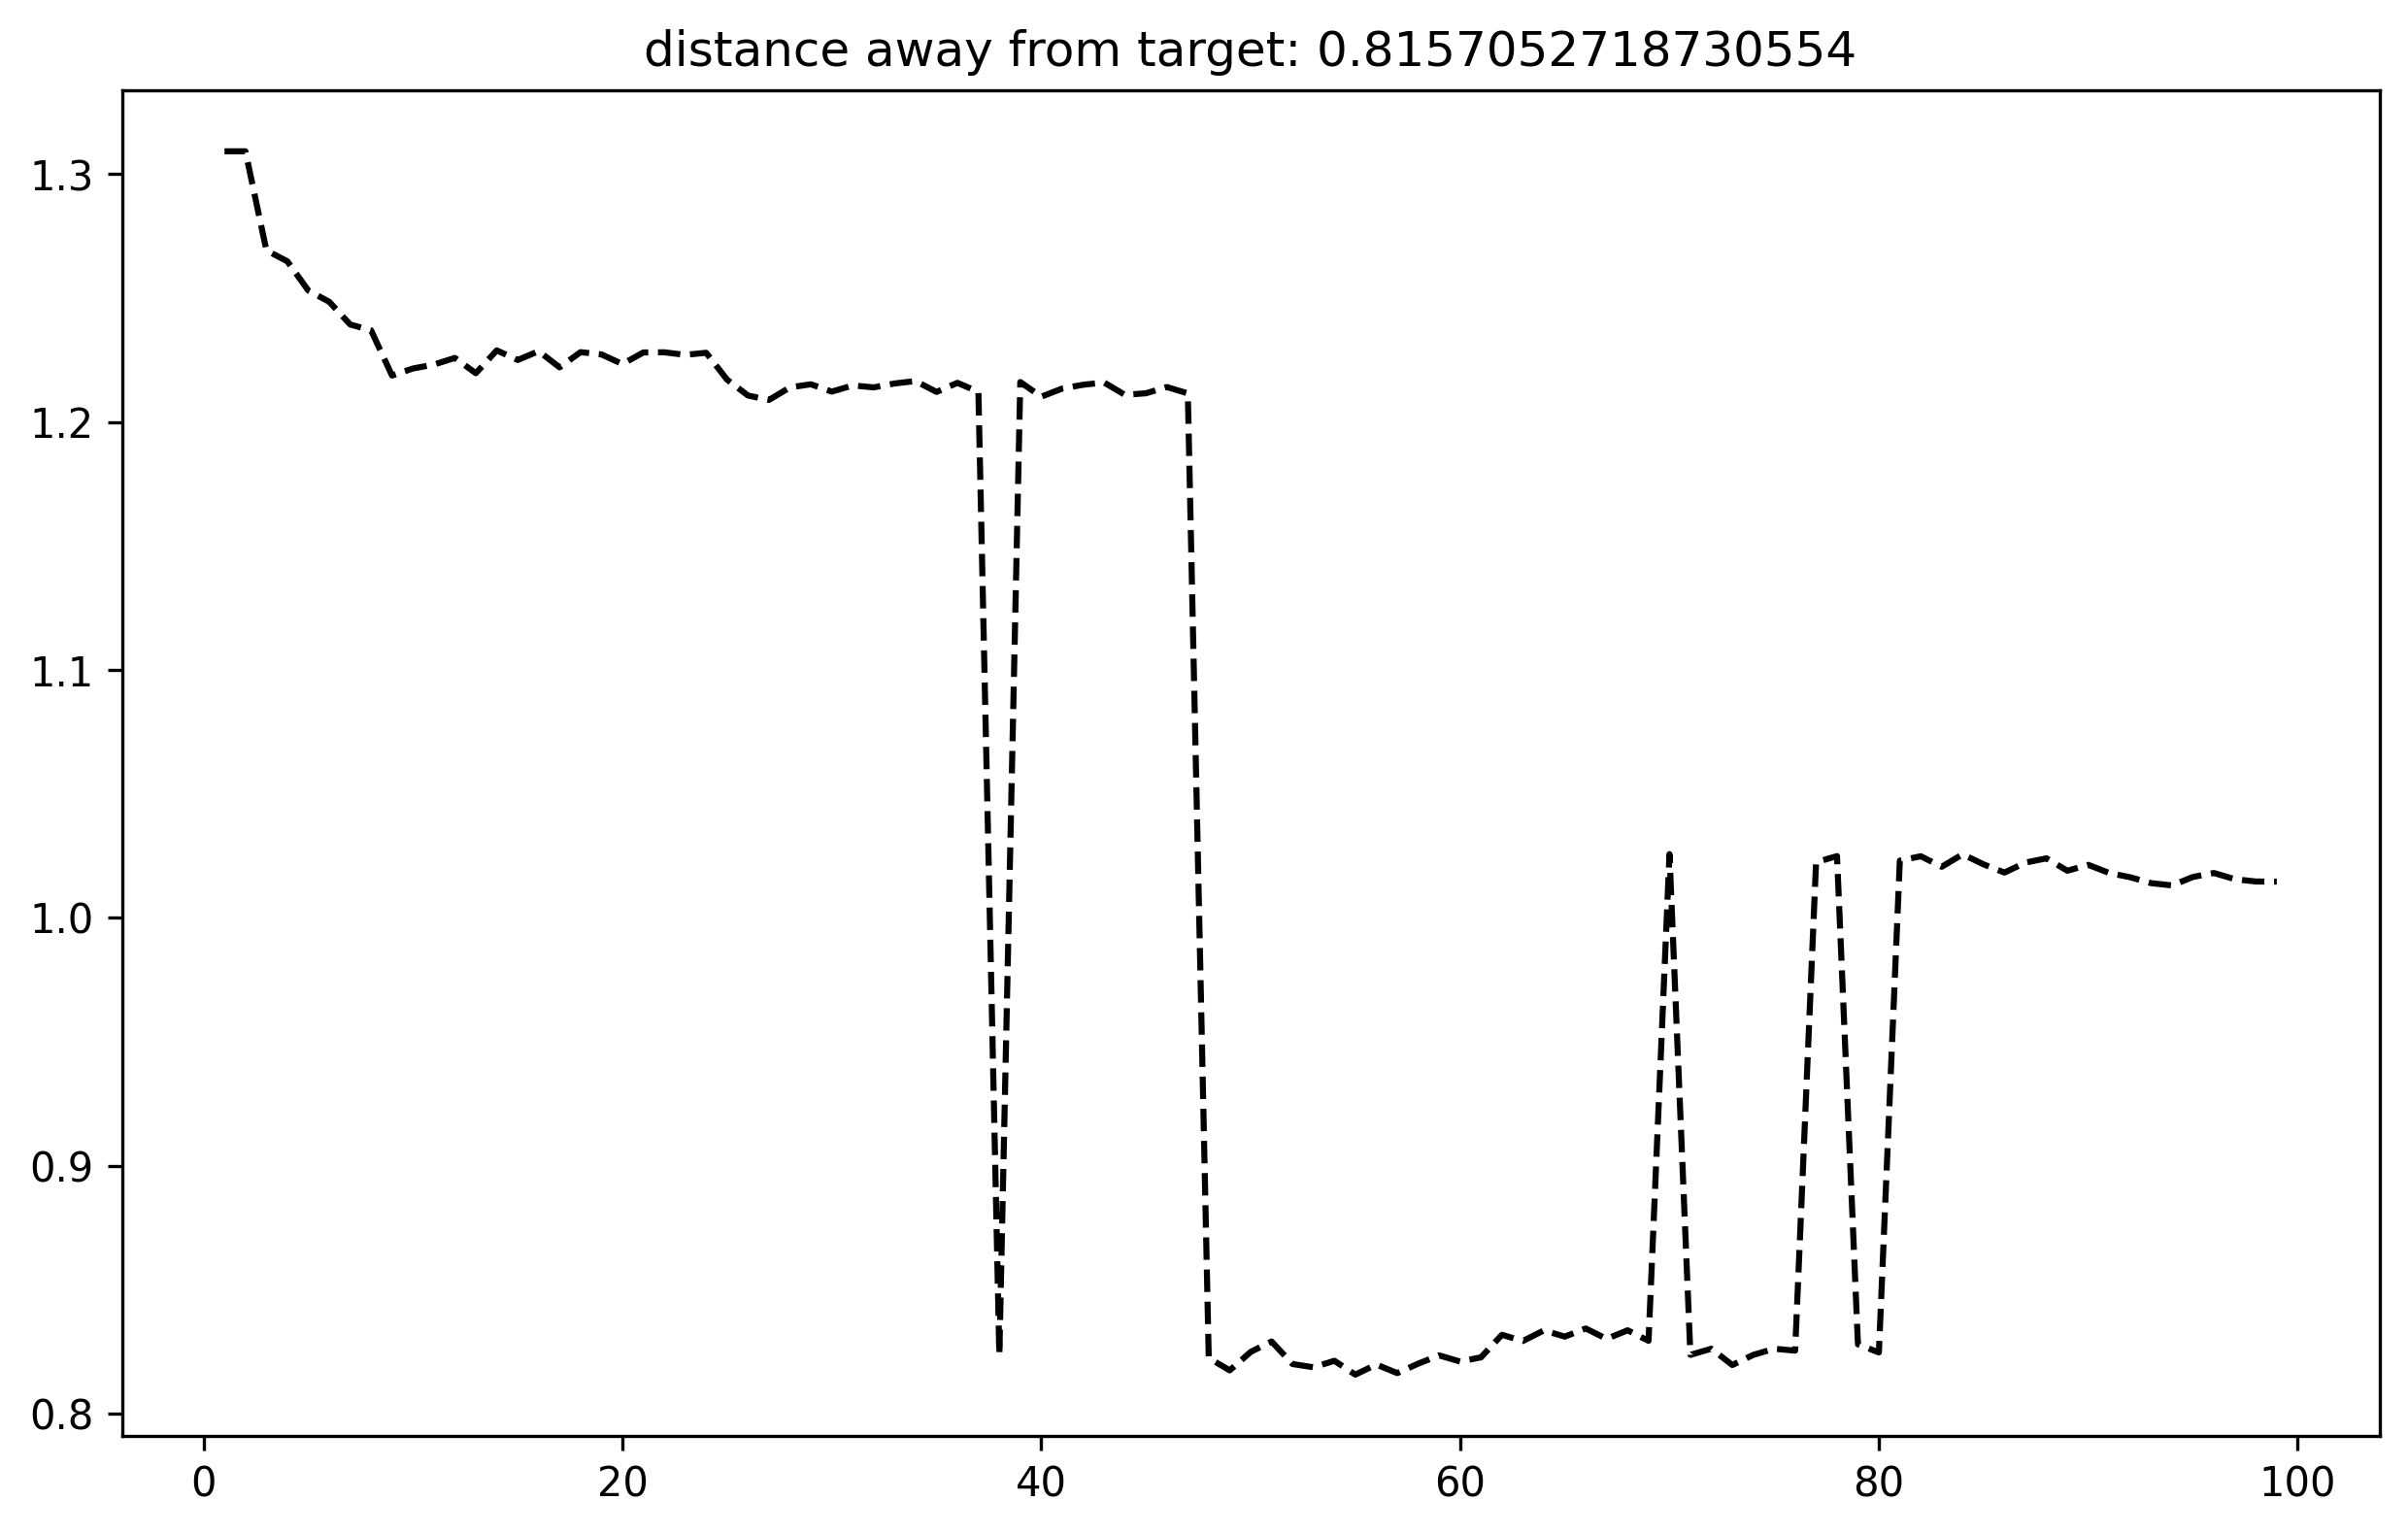
\includegraphics[width=\textwidth]{figures/filtered/knn_custom_15.png}
		\caption*{AGT (Filtered): 15×15m}
	\end{minipage}
	\hfill
	\begin{minipage}{0.49\textwidth}
		\centering
		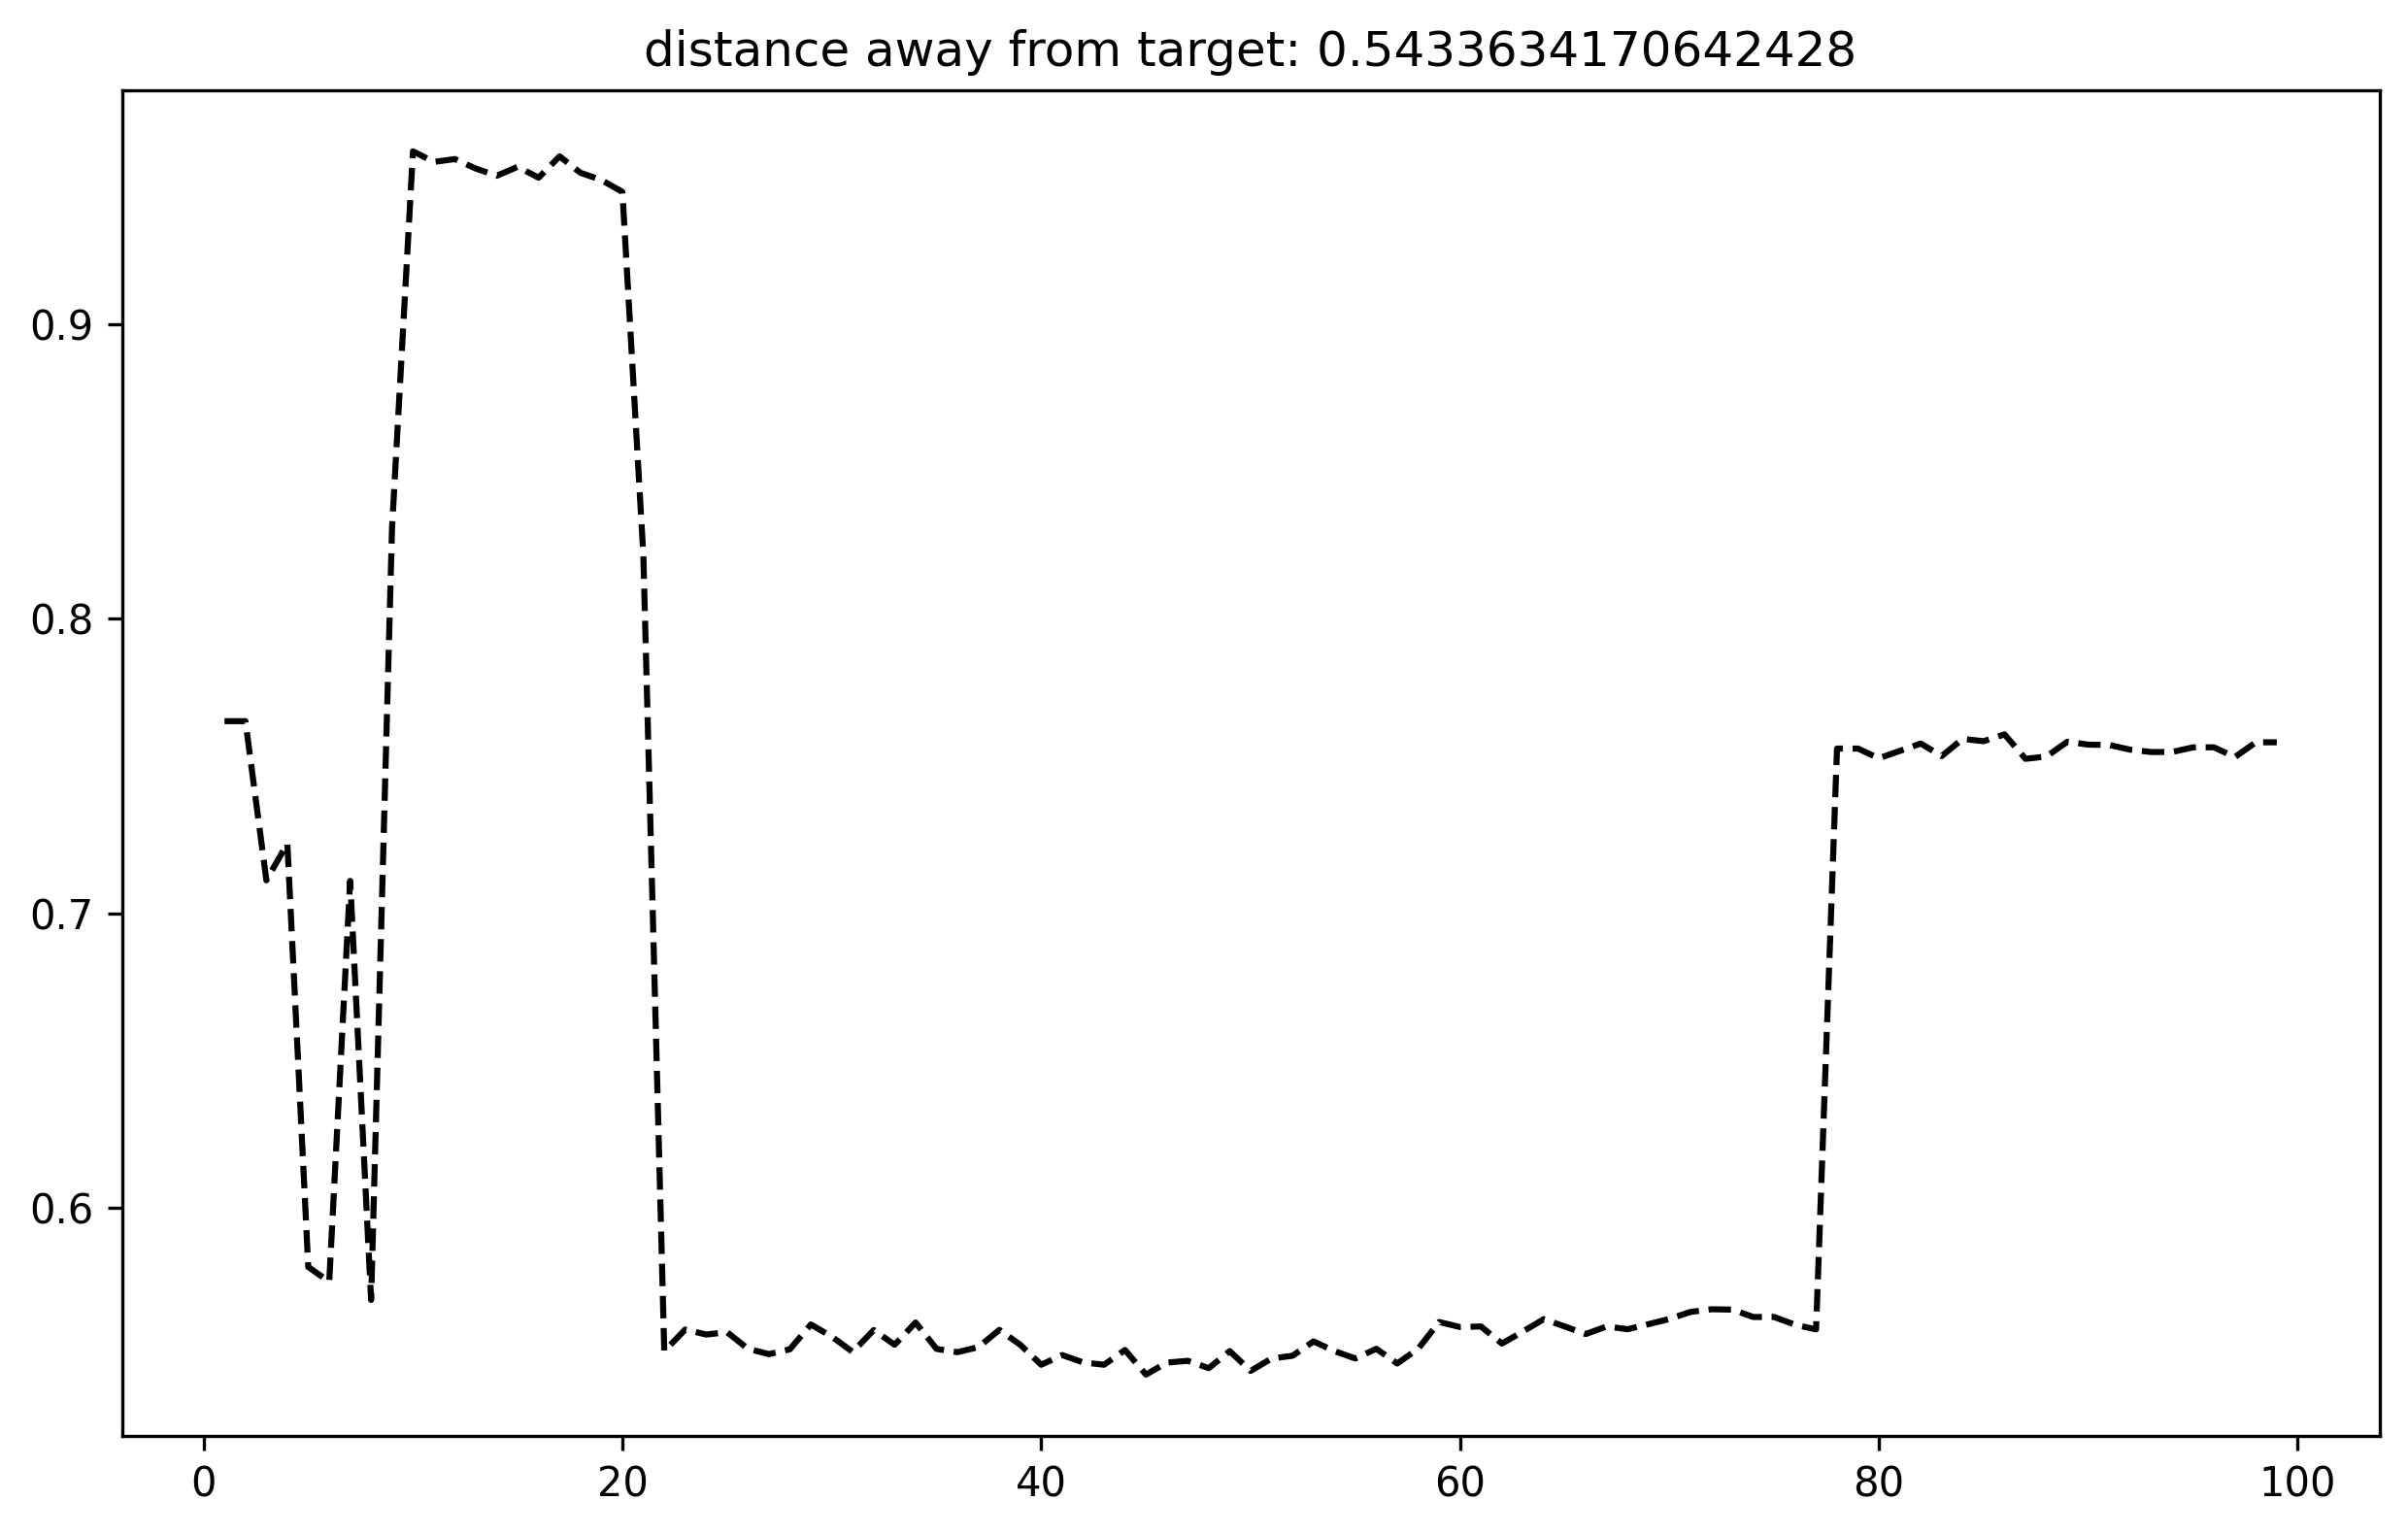
\includegraphics[width=\textwidth]{figures/unfiltered/knn_custom_15.png}
		\caption*{AGT (Unfiltered): 15×15m}
	\end{minipage}
\end{figure}

\clearpage

\subsection*{MLP}

\begin{figure}[H]
	\centering
	\begin{minipage}{0.49\textwidth}
		\centering
		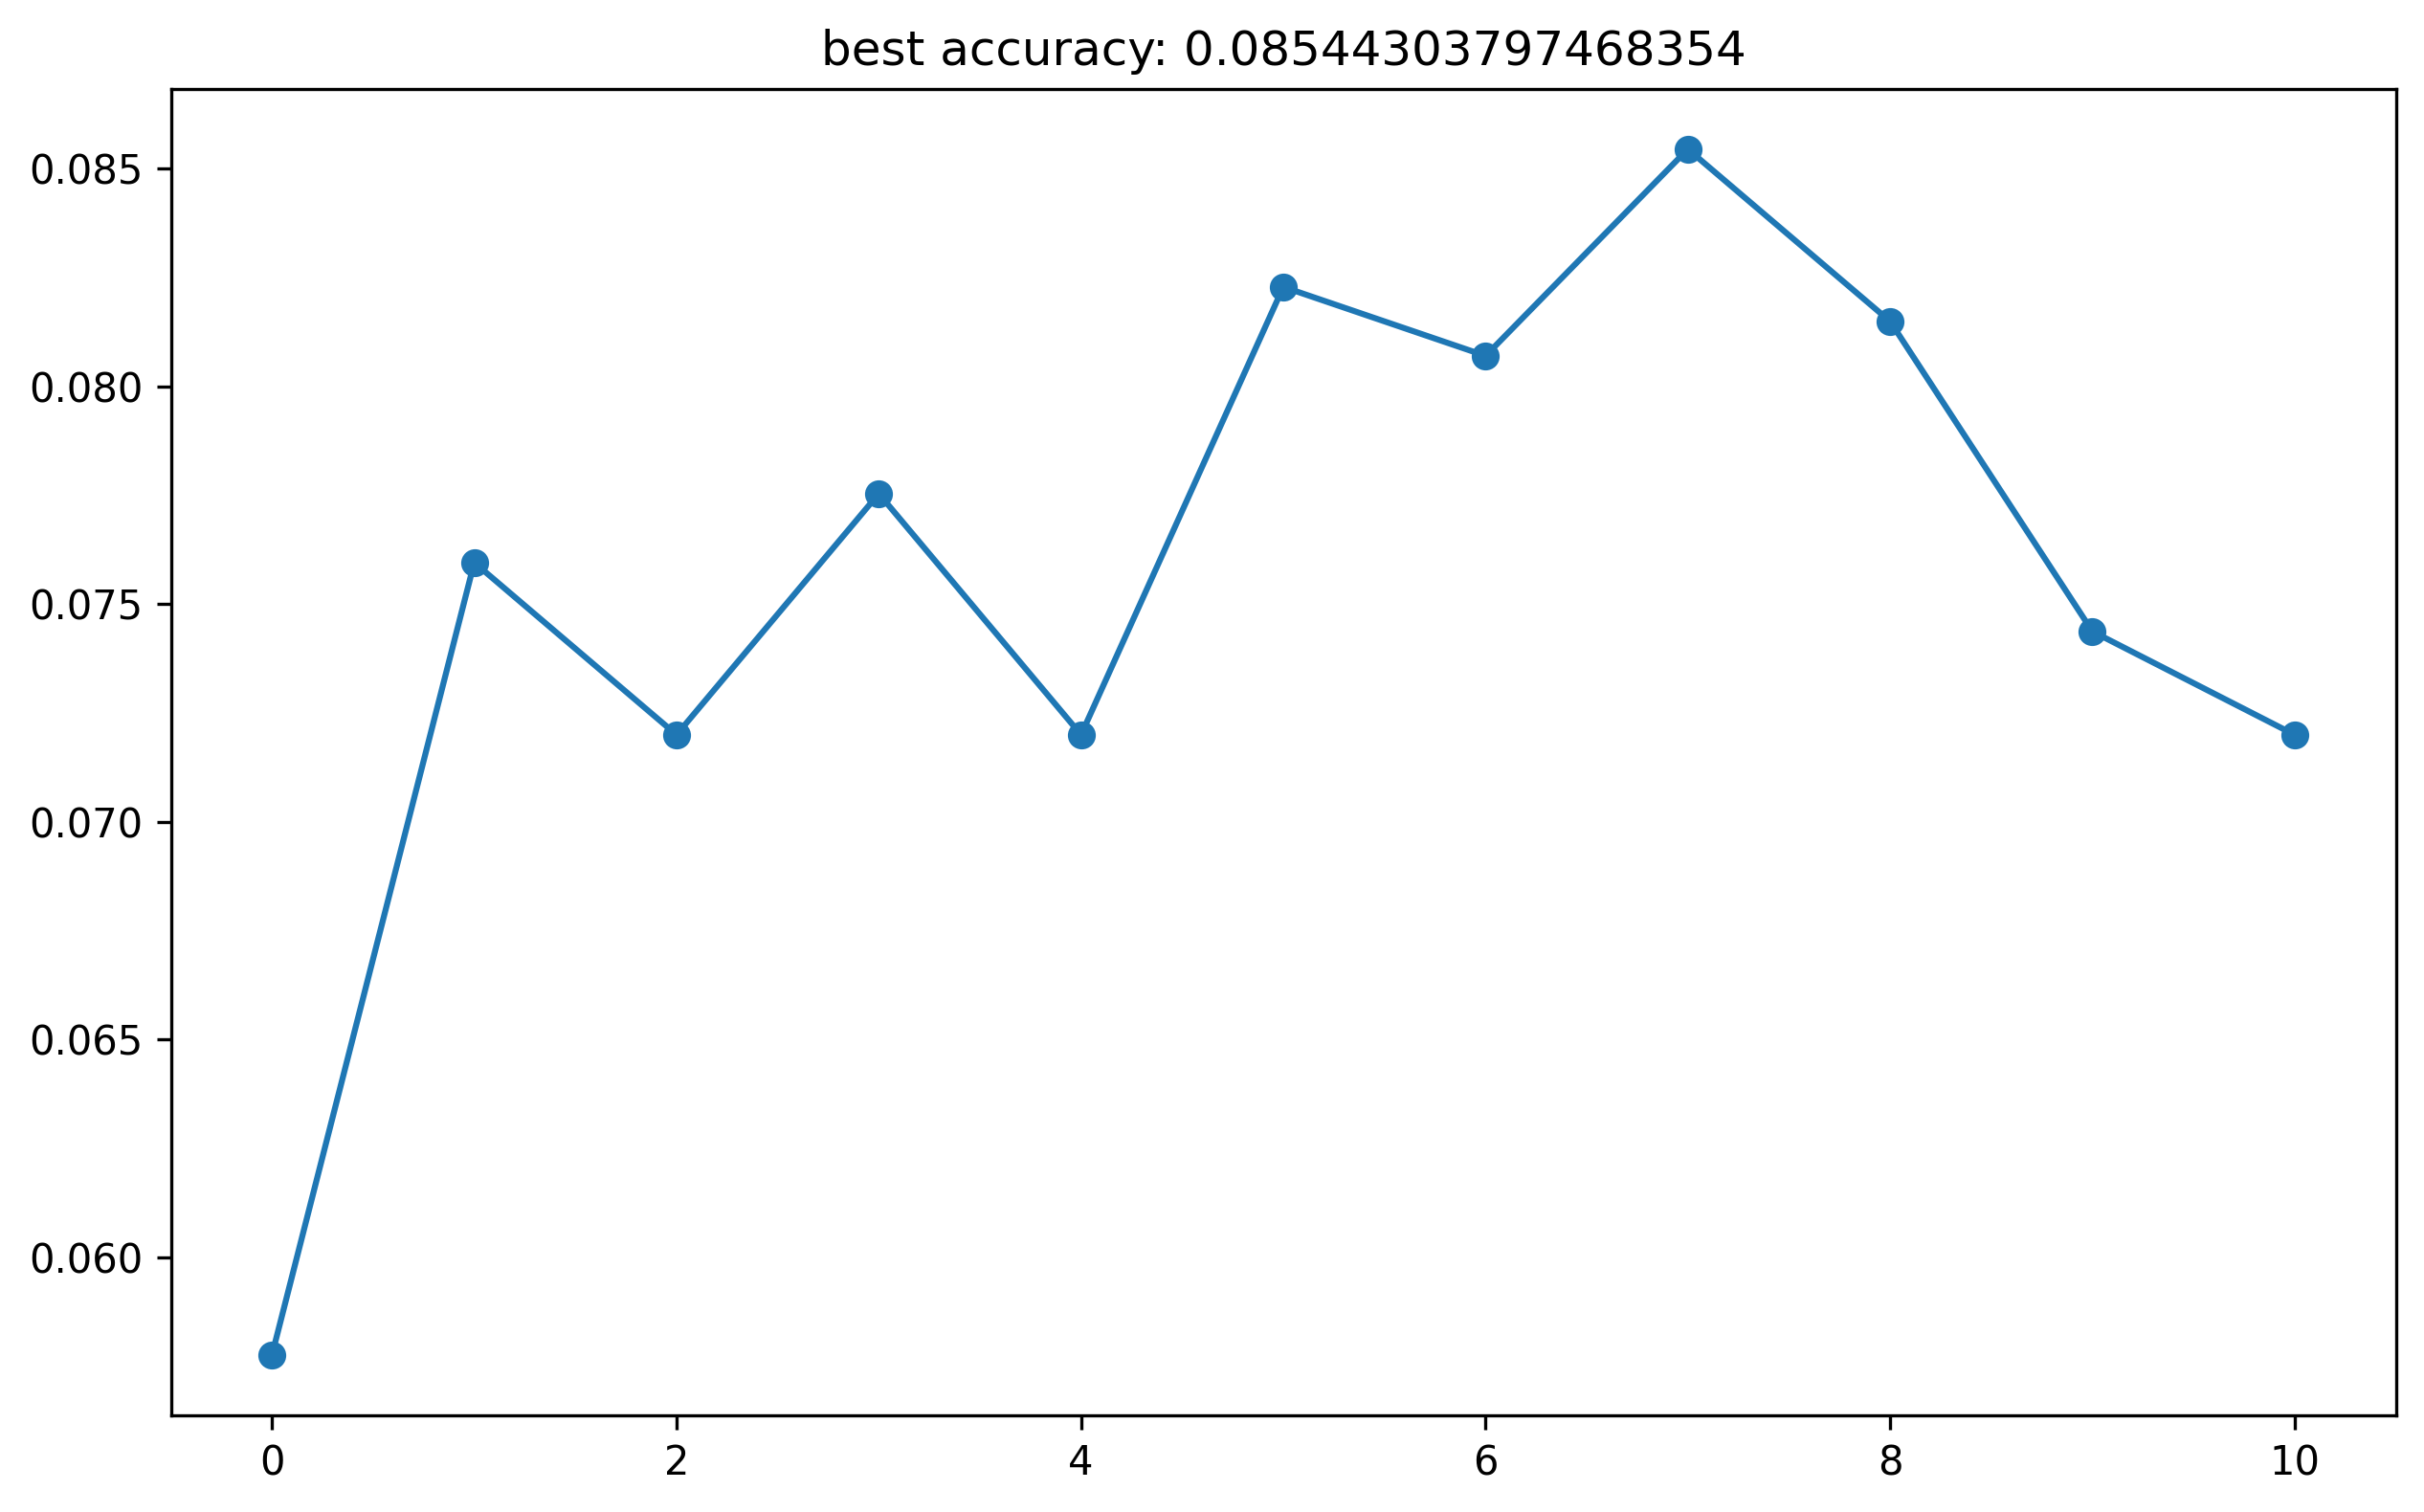
\includegraphics[width=\textwidth]{figures/filtered/mlp_acc_1.png}
		\caption*{Accuracy (Filtered): 1×1m}
	\end{minipage}
	\hfill
	\begin{minipage}{0.49\textwidth}
		\centering
		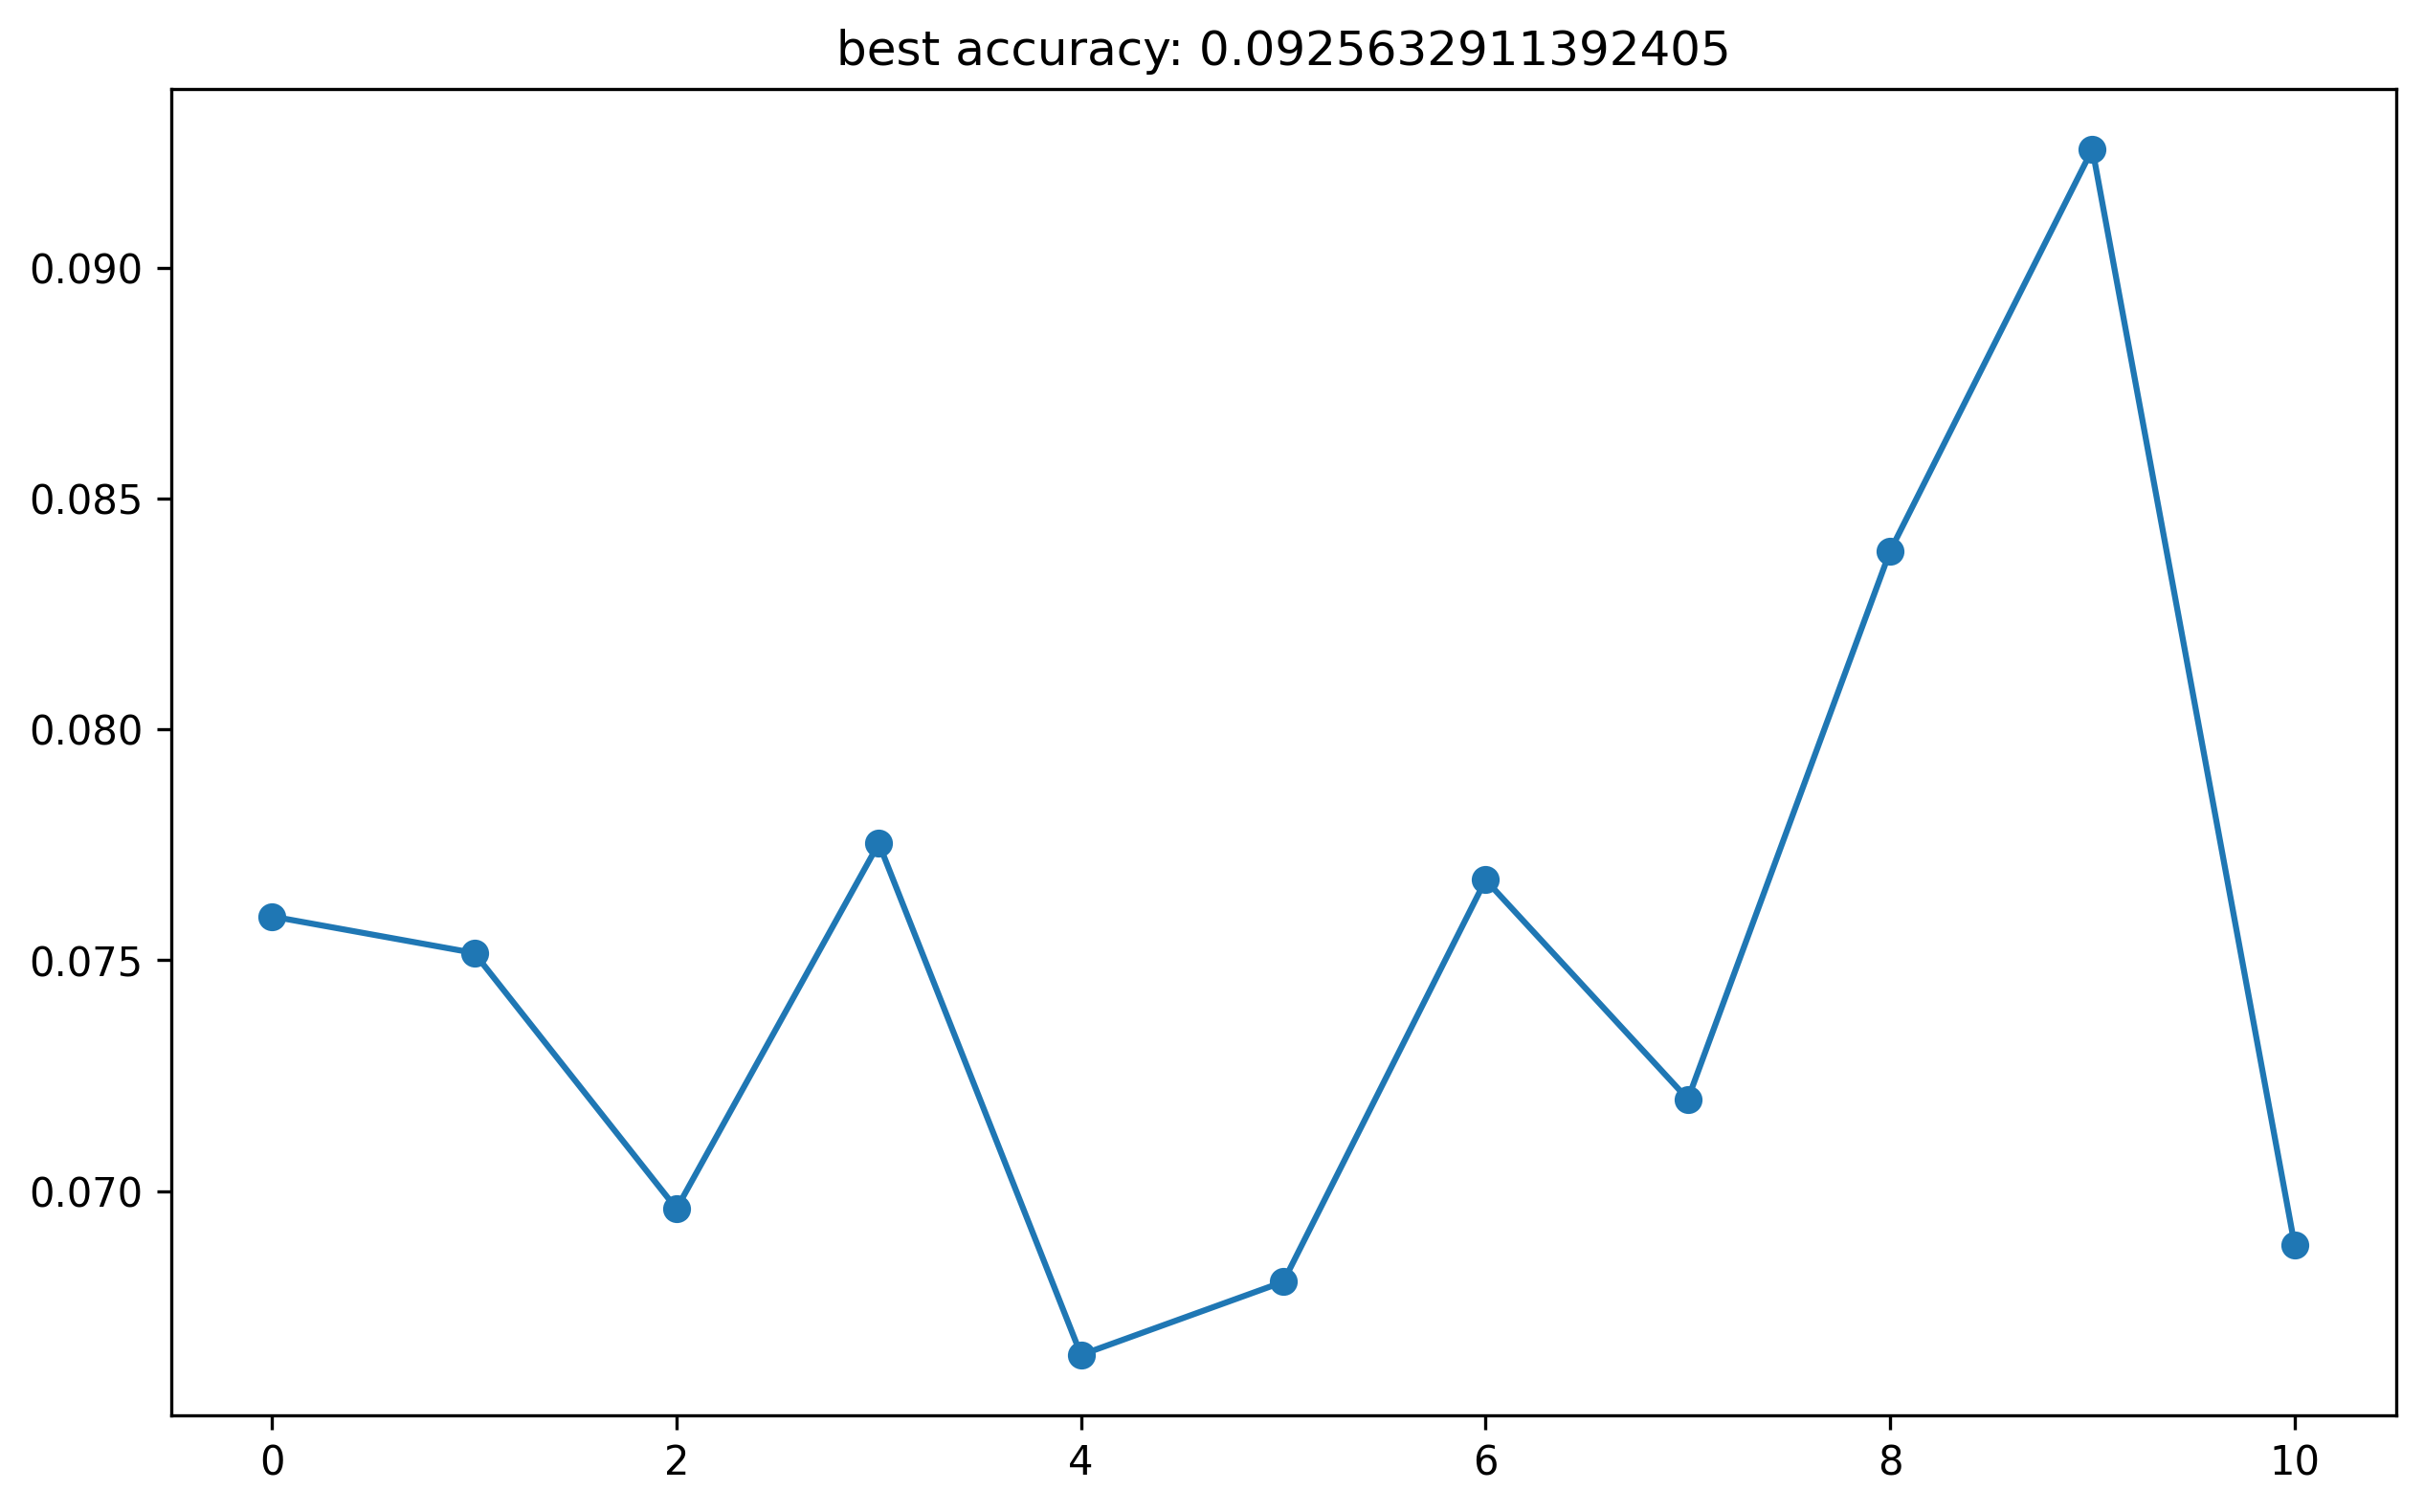
\includegraphics[width=\textwidth]{figures/unfiltered/mlp_acc_1.png}
		\caption*{Accuracy (Unfiltered): 1×1m}
	\end{minipage}
\end{figure}

\begin{figure}[H]
	\centering
	\begin{minipage}{0.49\textwidth}
		\centering
		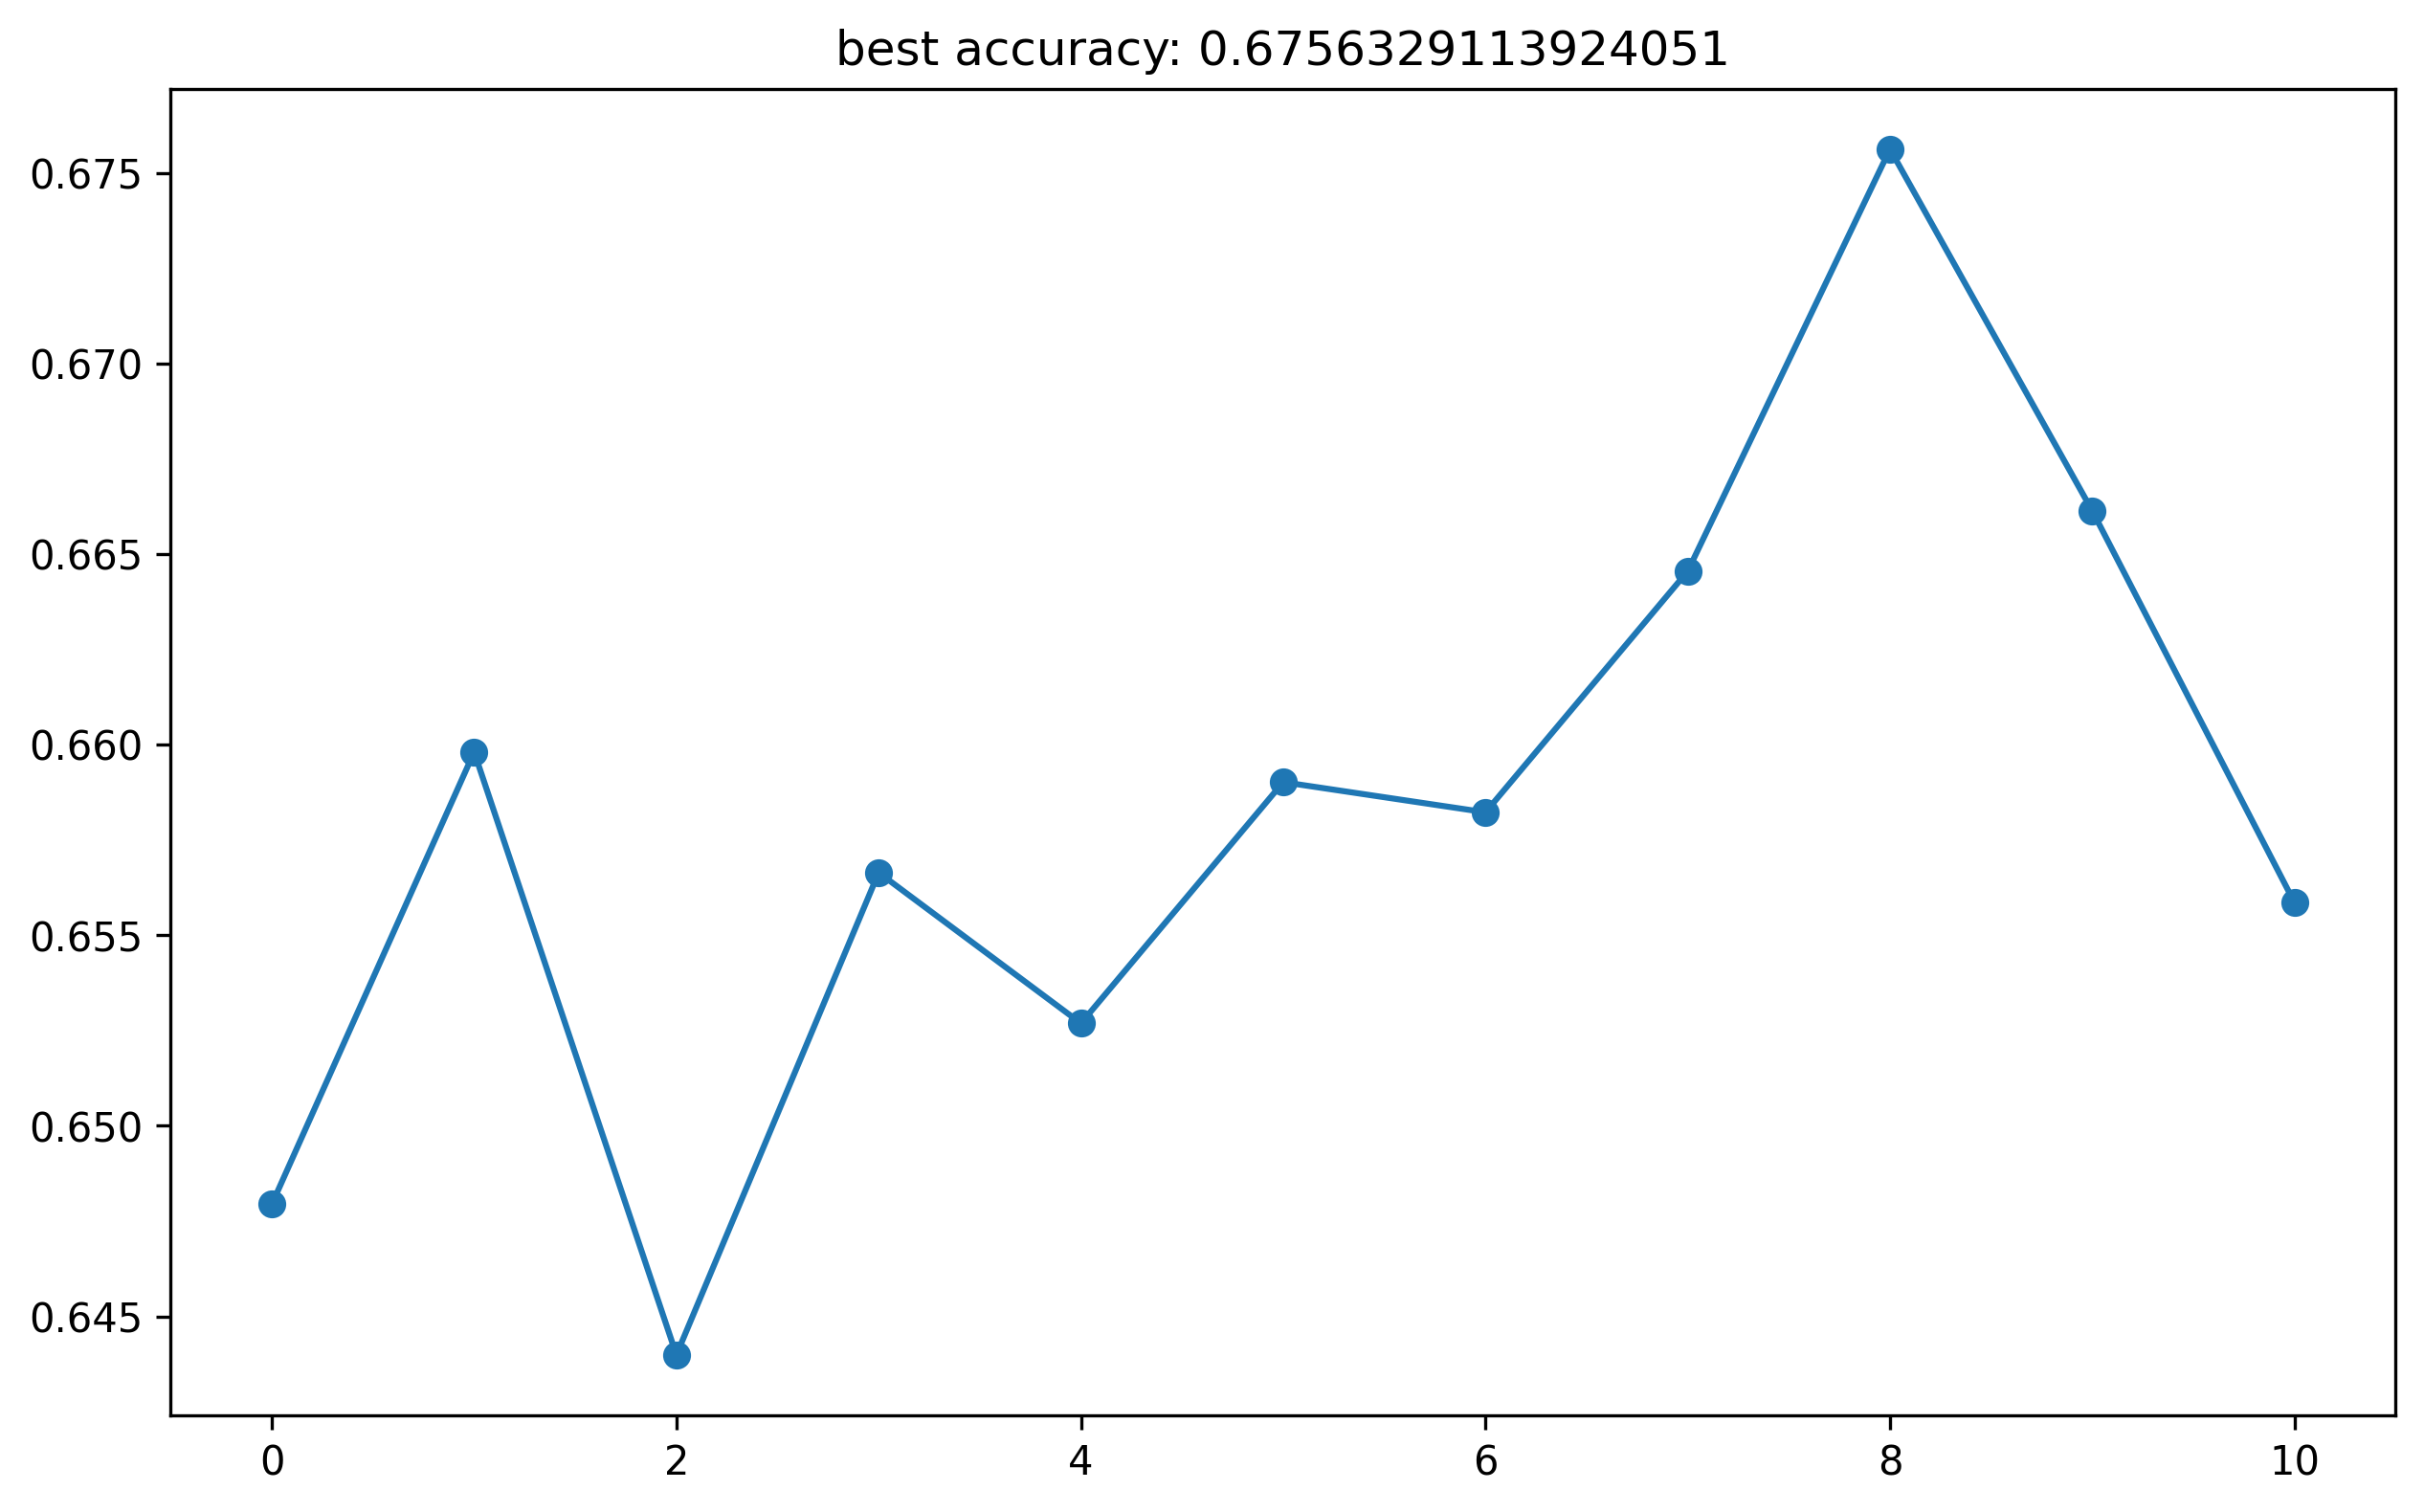
\includegraphics[width=\textwidth]{figures/filtered/mlp_acc_7.png}
		\caption*{Accuracy (Filtered): 7×7m}
	\end{minipage}
	\hfill
	\begin{minipage}{0.49\textwidth}
		\centering
		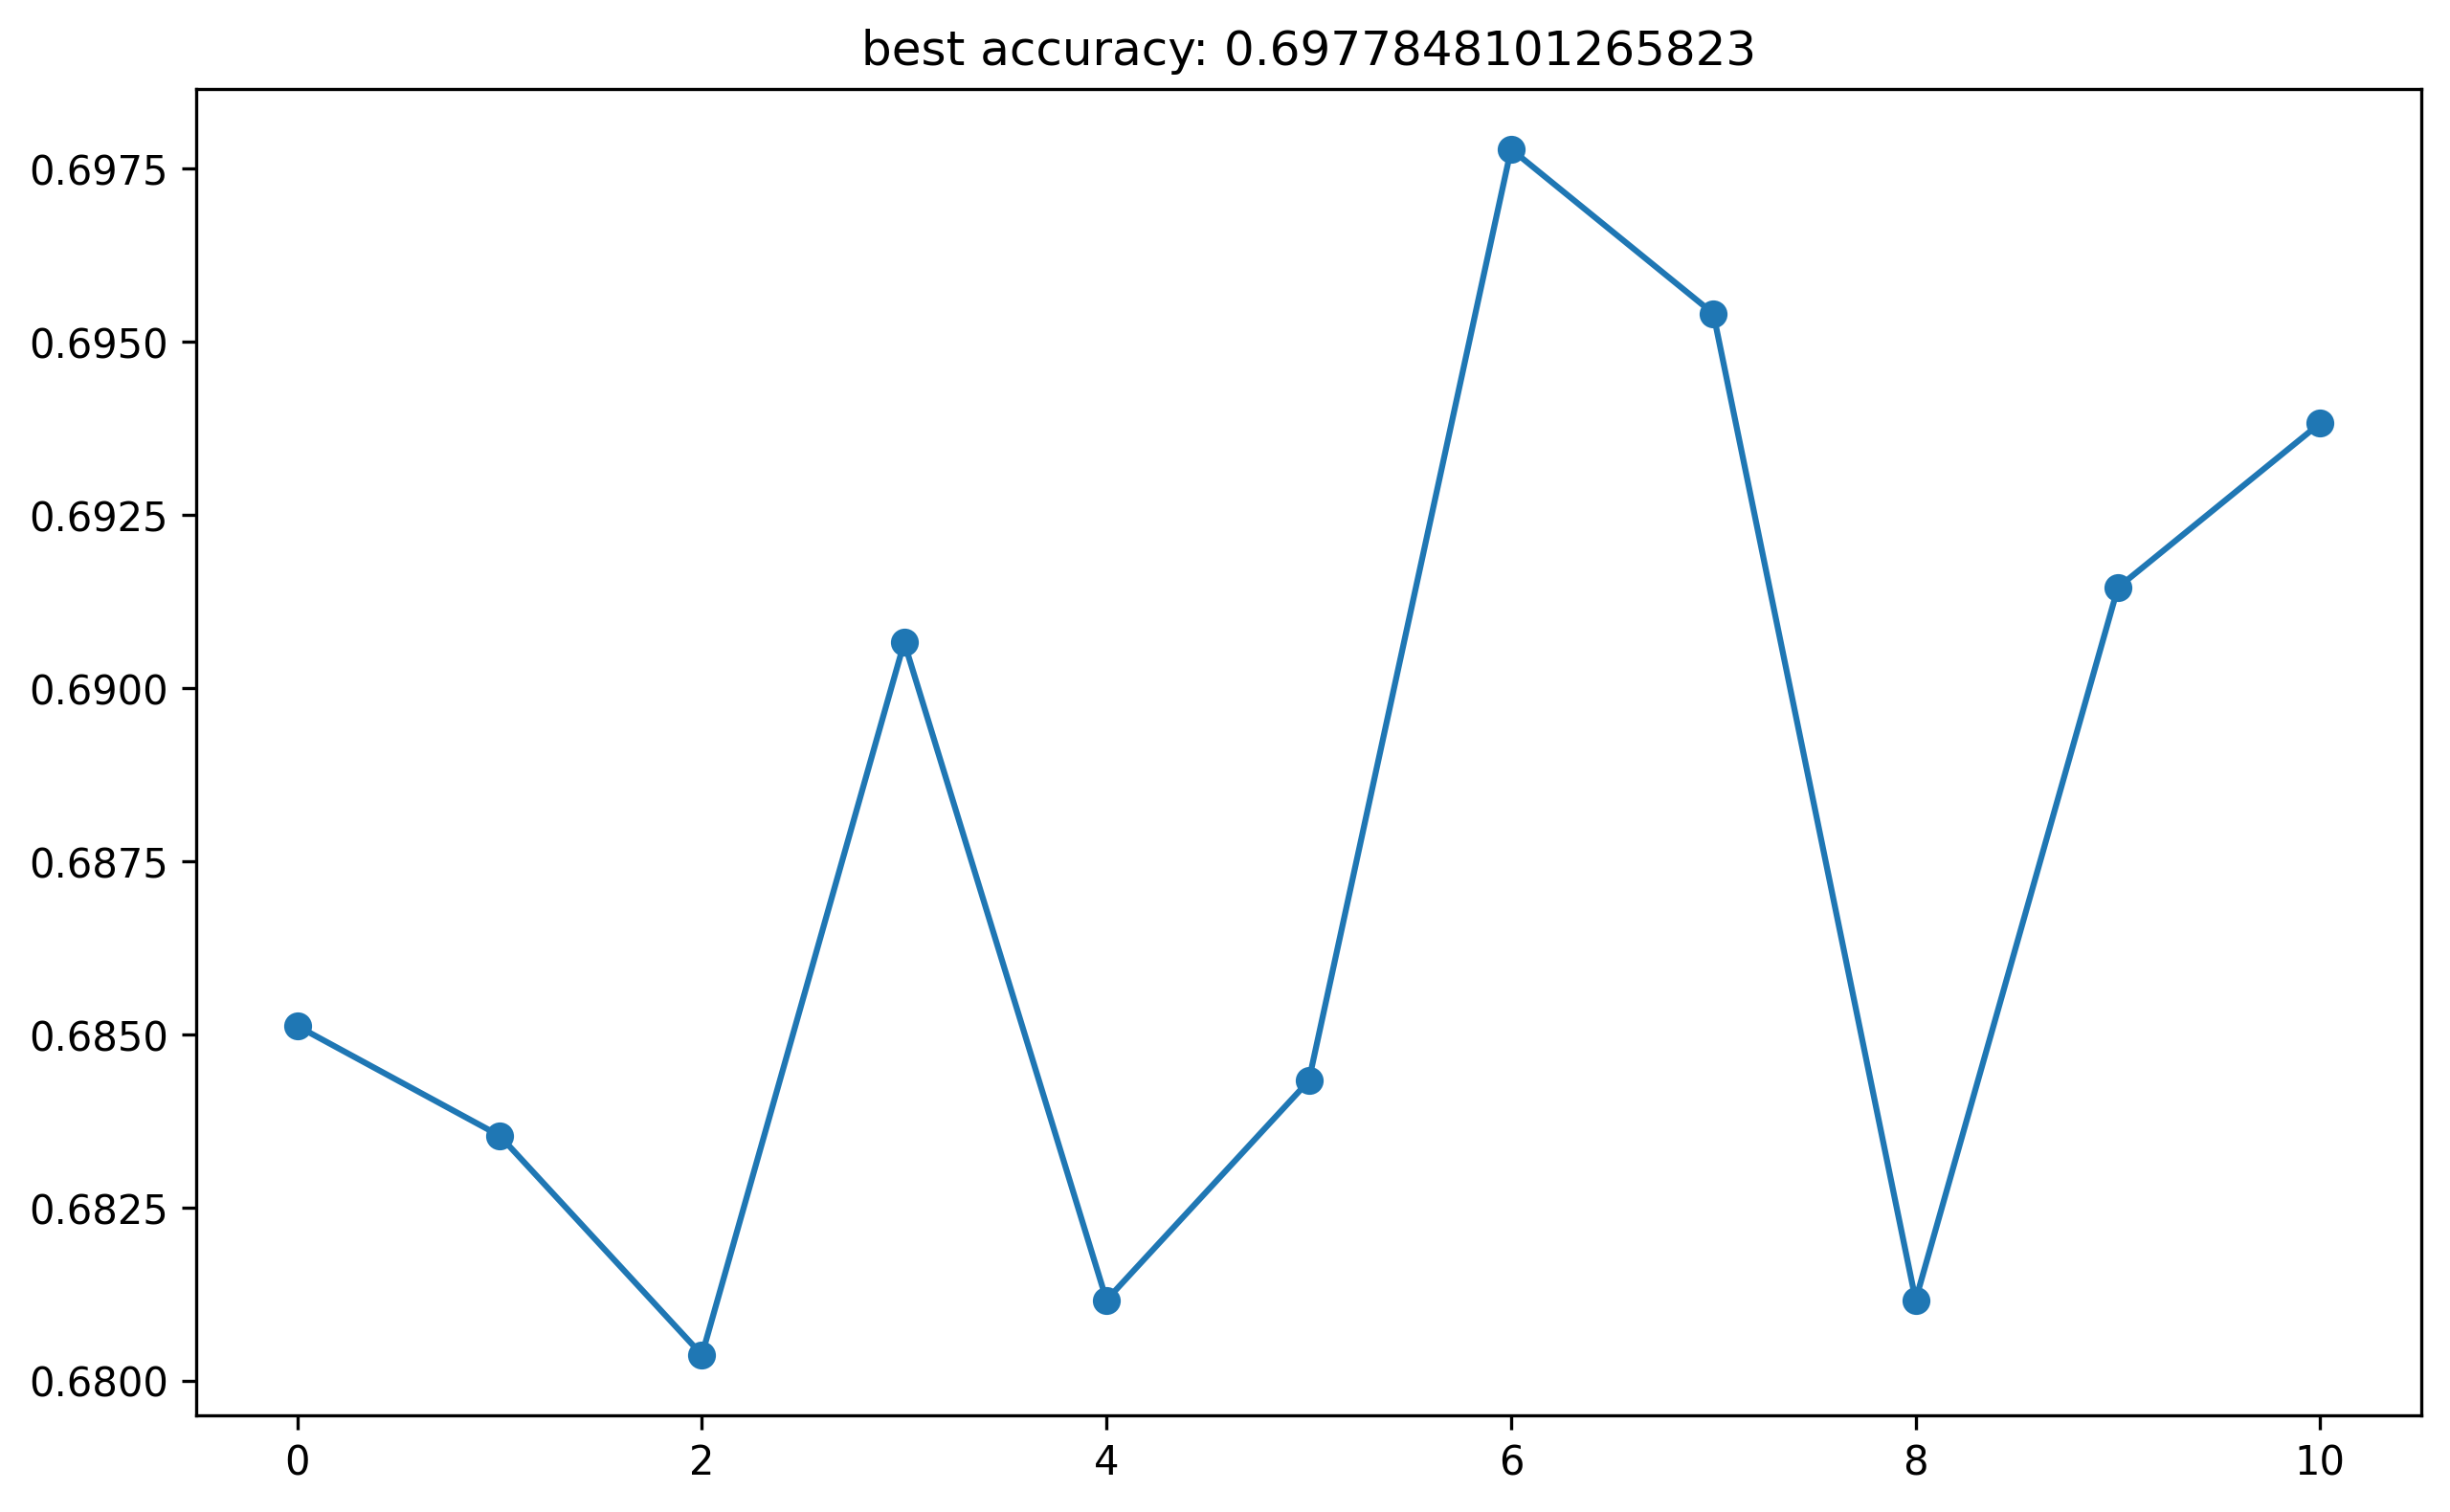
\includegraphics[width=\textwidth]{figures/unfiltered/mlp_acc_7.png}
		\caption*{Accuracy (Unfiltered): 7×7m}
	\end{minipage}
\end{figure}

\begin{figure}[H]
	\centering
	\begin{minipage}{0.49\textwidth}
		\centering
		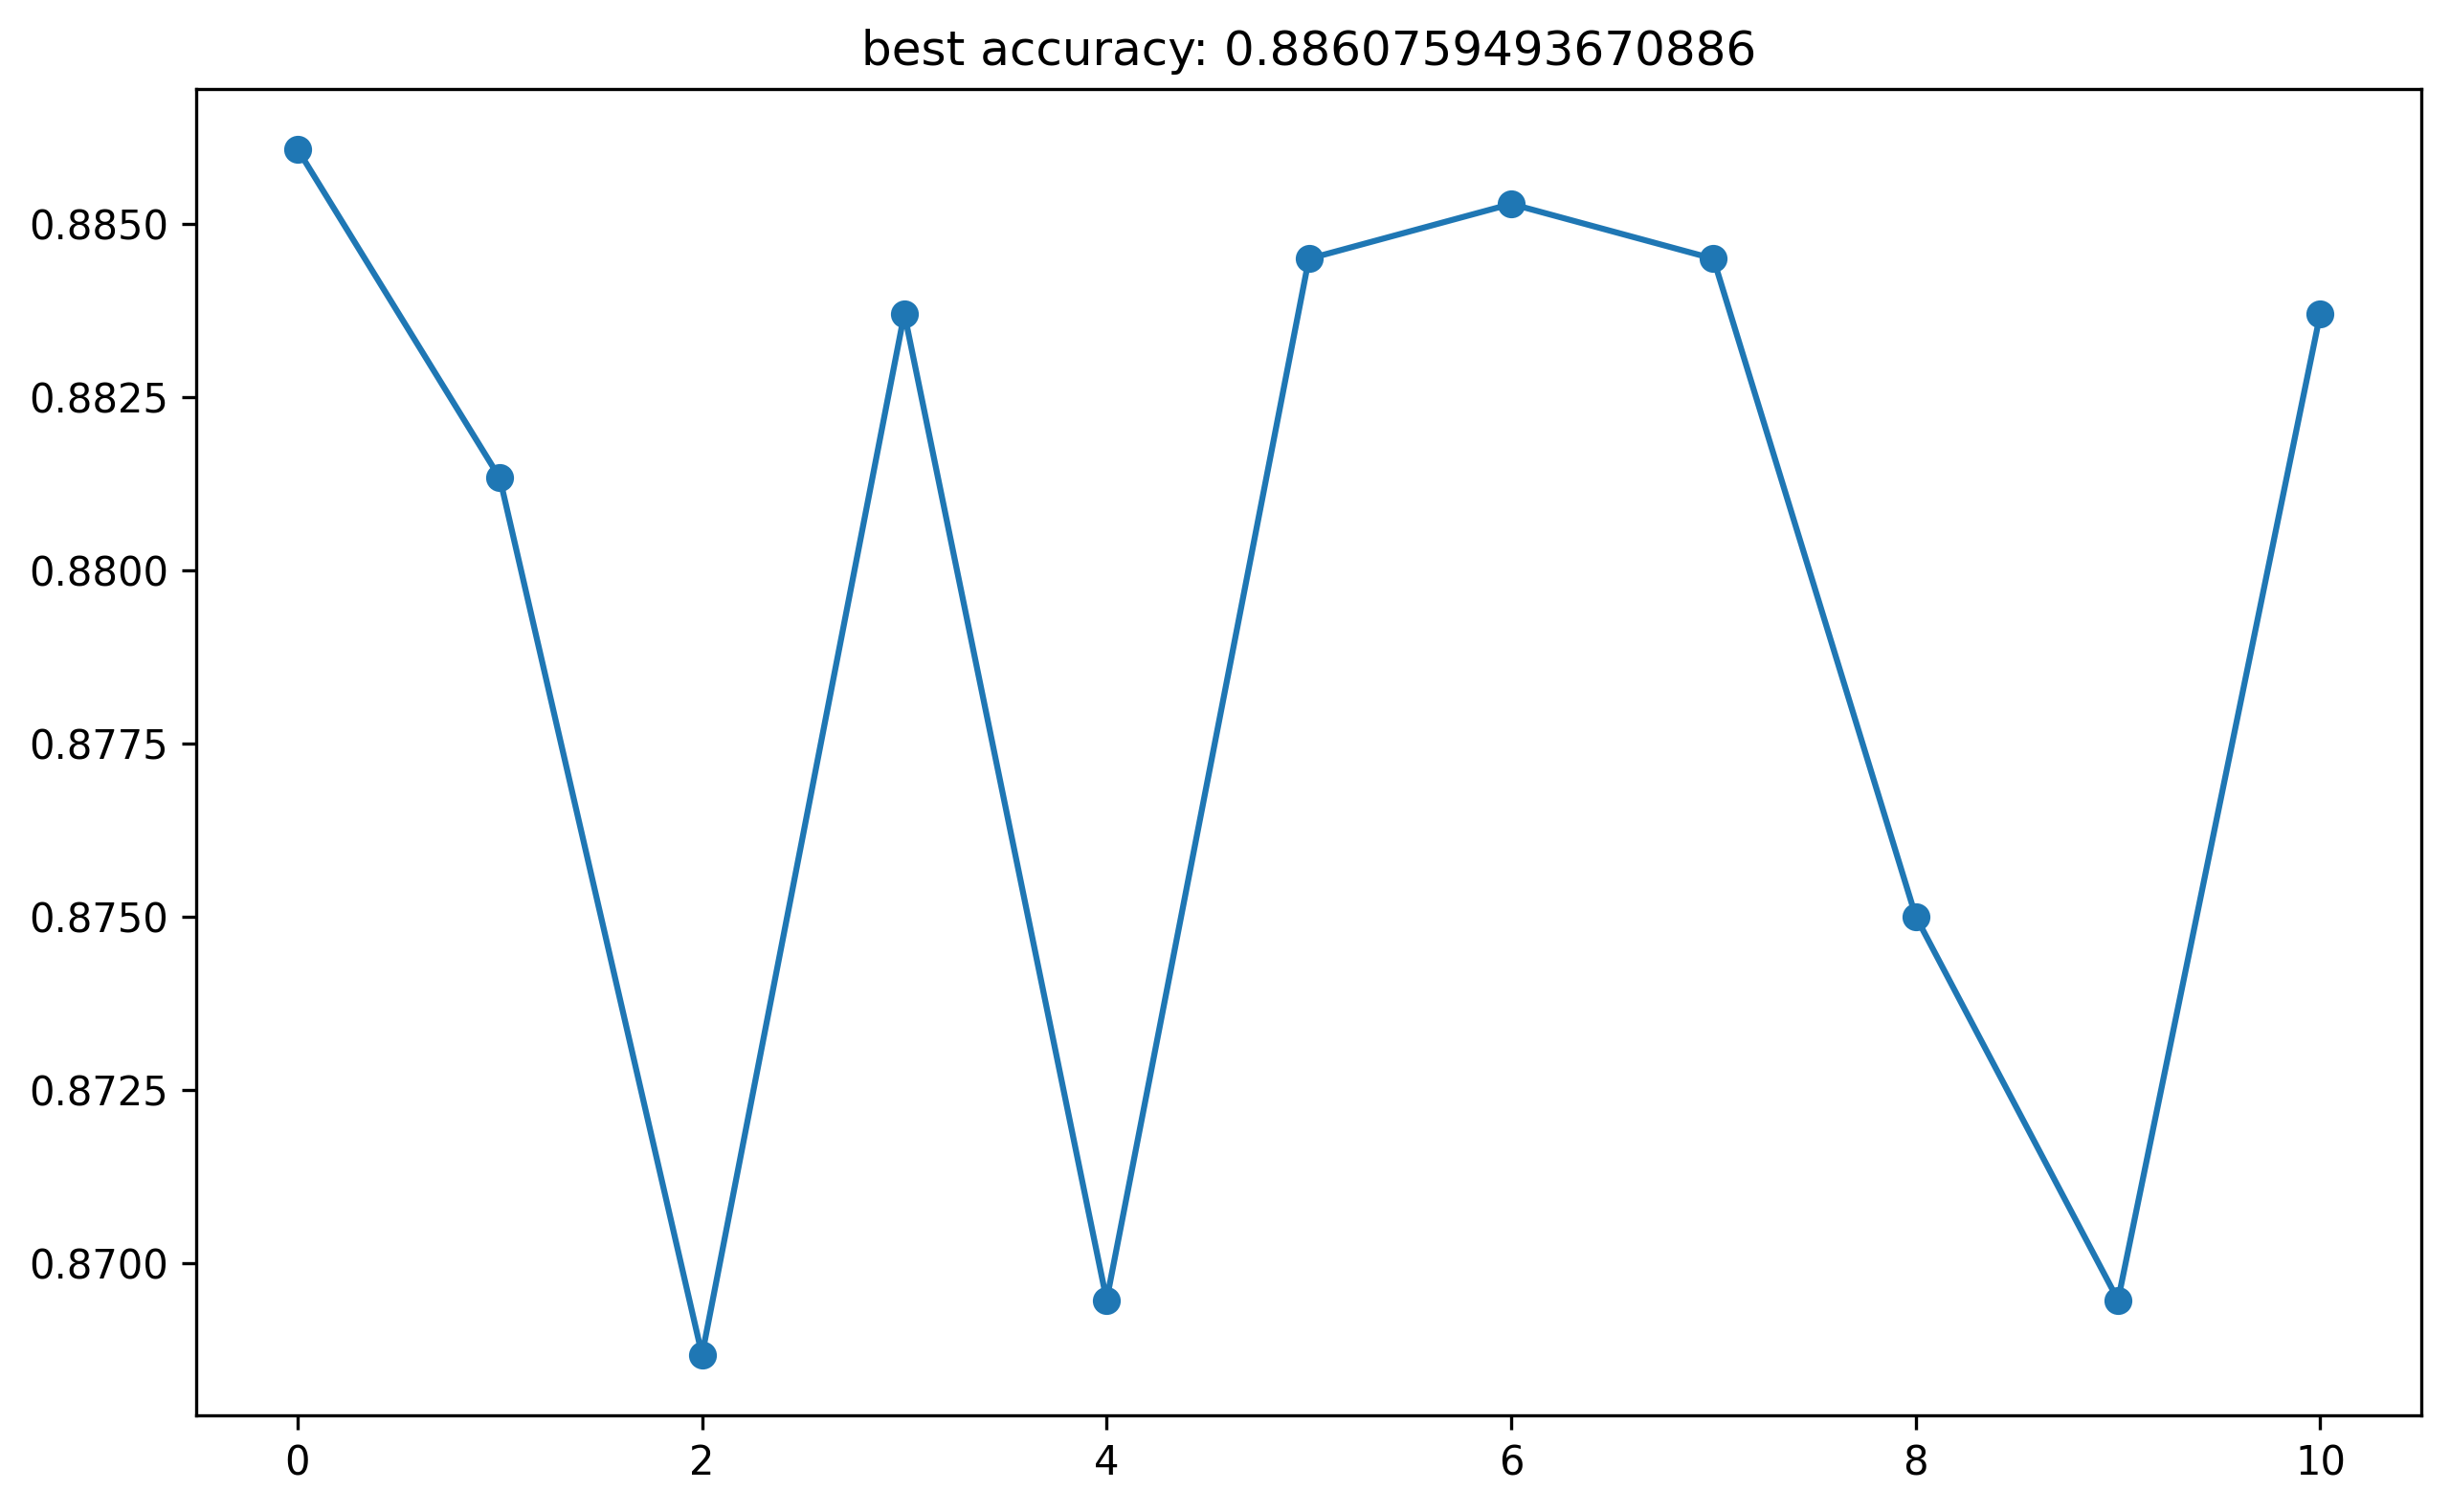
\includegraphics[width=\textwidth]{figures/filtered/mlp_acc_15.png}
		\caption*{Accuracy (Filtered): 15×15m}
	\end{minipage}
	\hfill
	\begin{minipage}{0.49\textwidth}
		\centering
		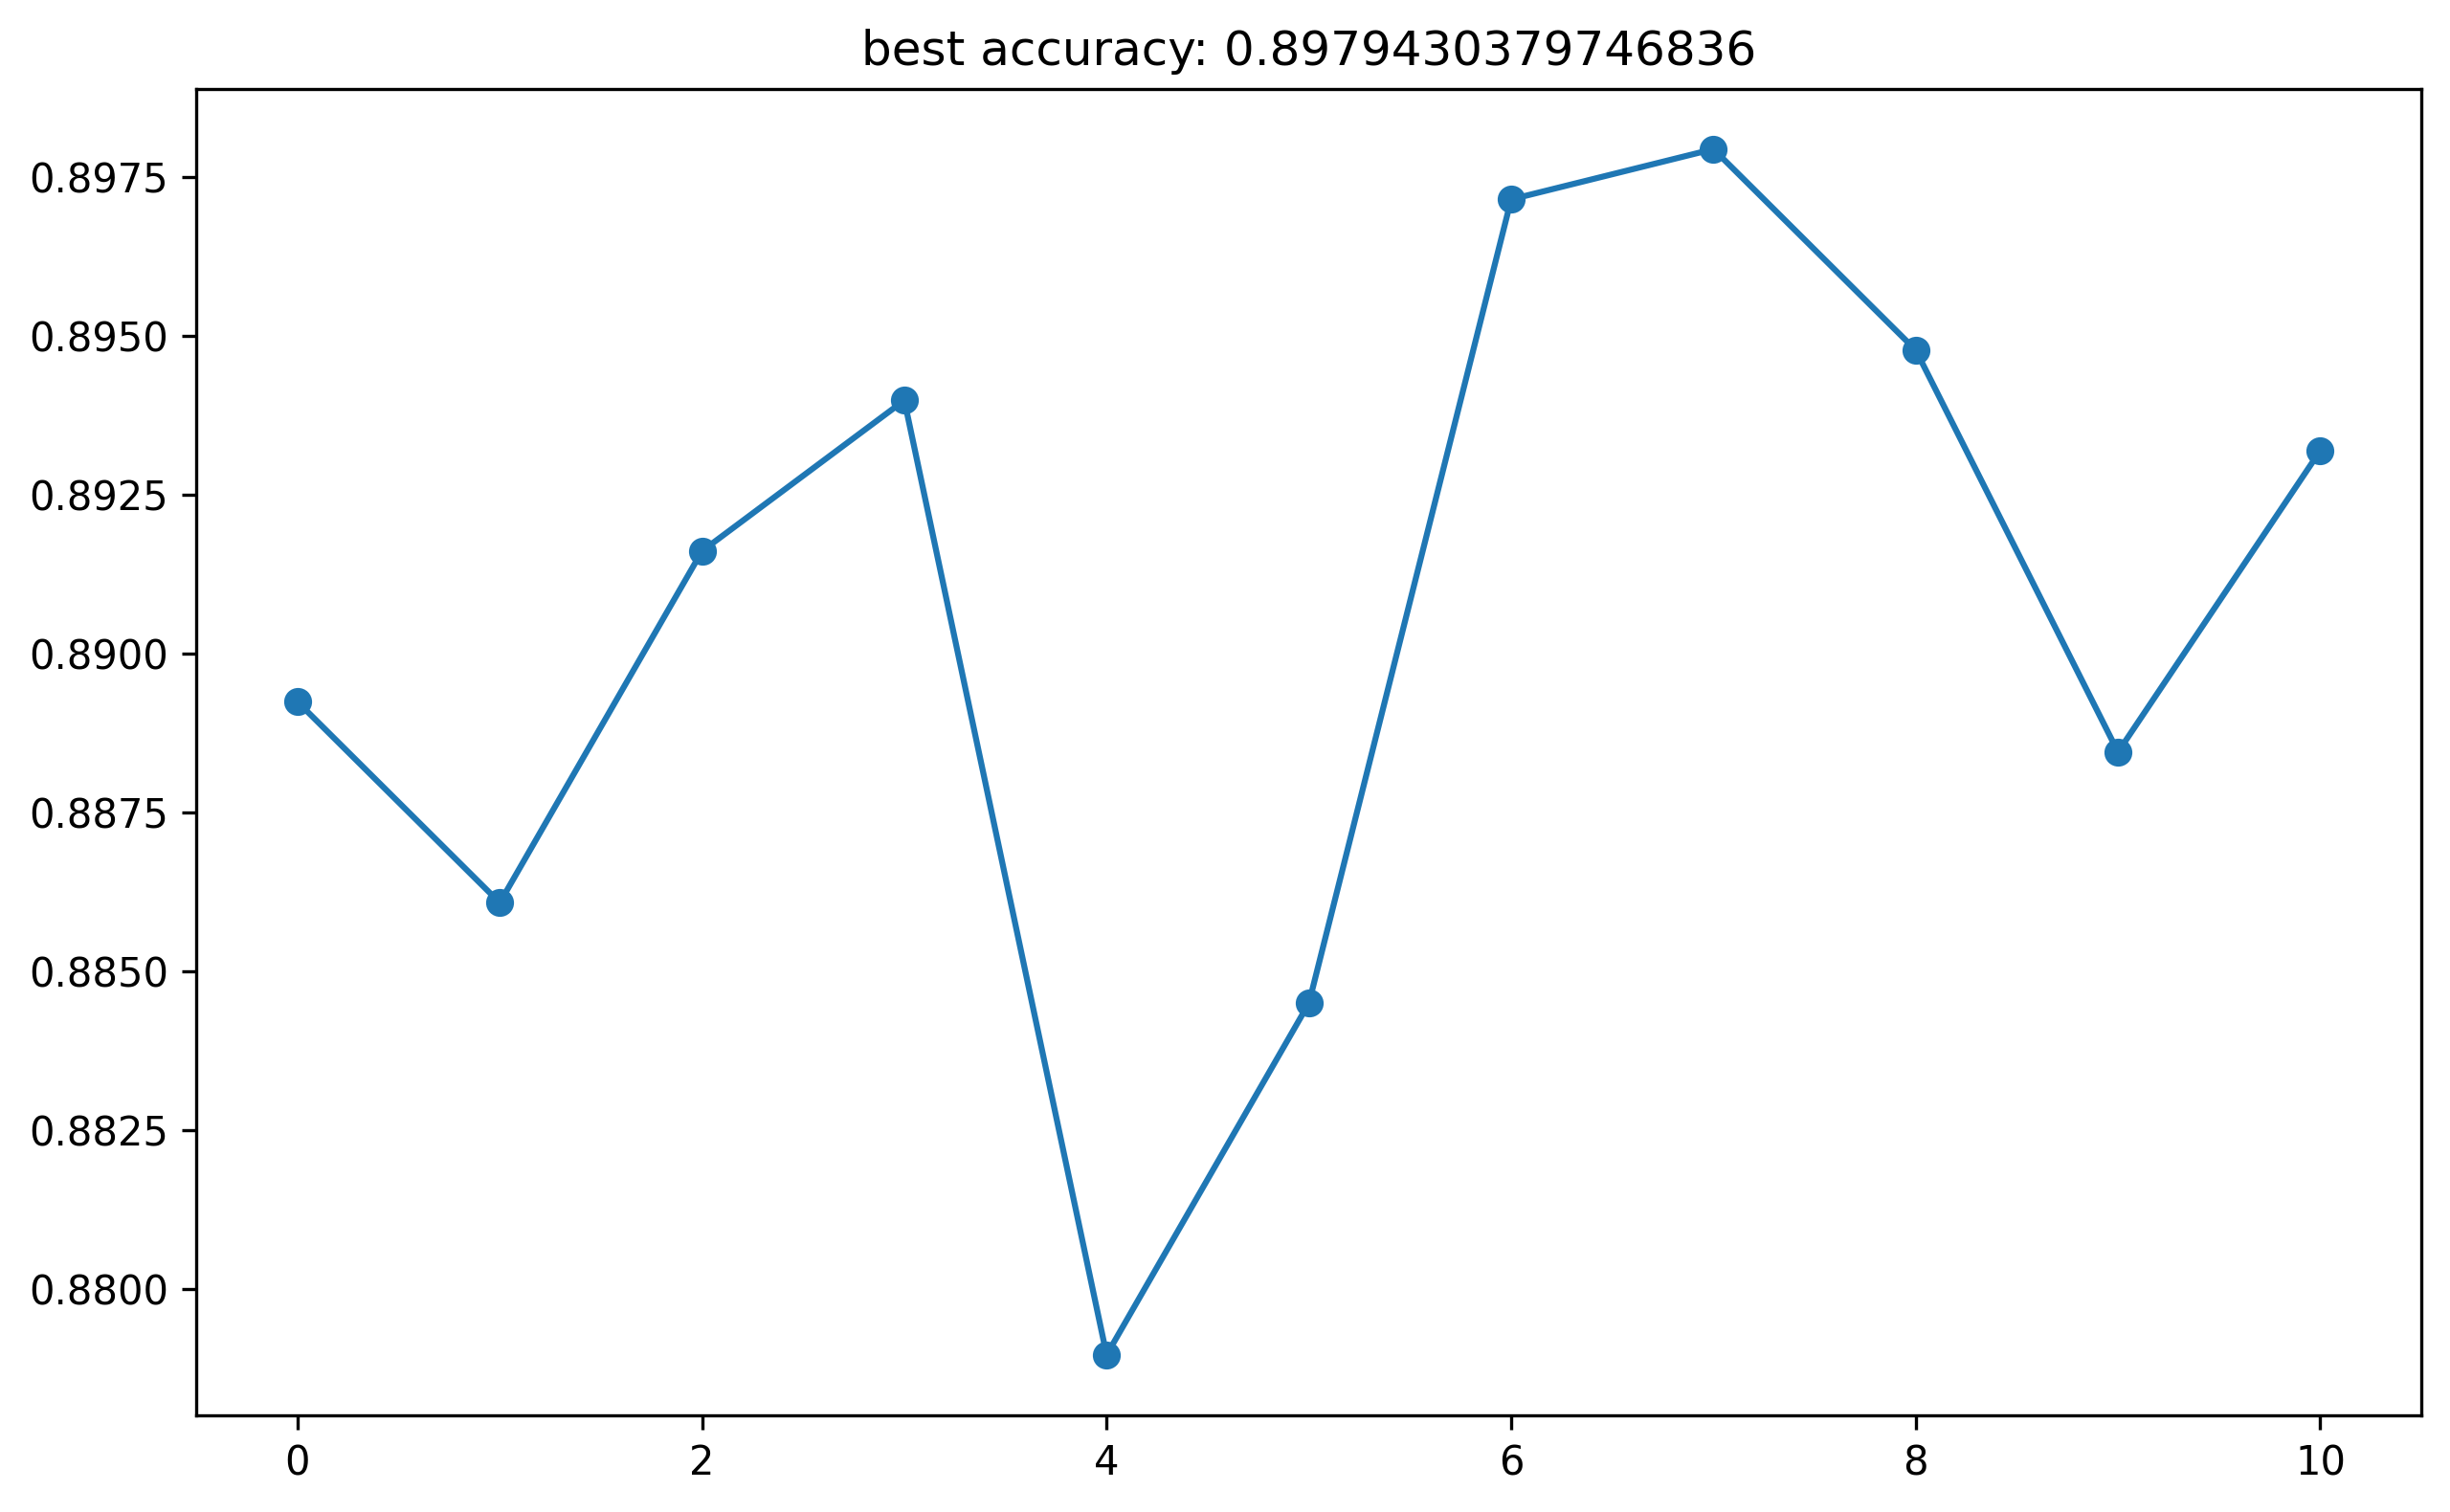
\includegraphics[width=\textwidth]{figures/unfiltered/mlp_acc_15.png}
		\caption*{Accuracy (Unfiltered): 15×15m}
	\end{minipage}
\end{figure}

\begin{figure}[H]
	\centering
	\begin{minipage}{0.49\textwidth}
		\centering
		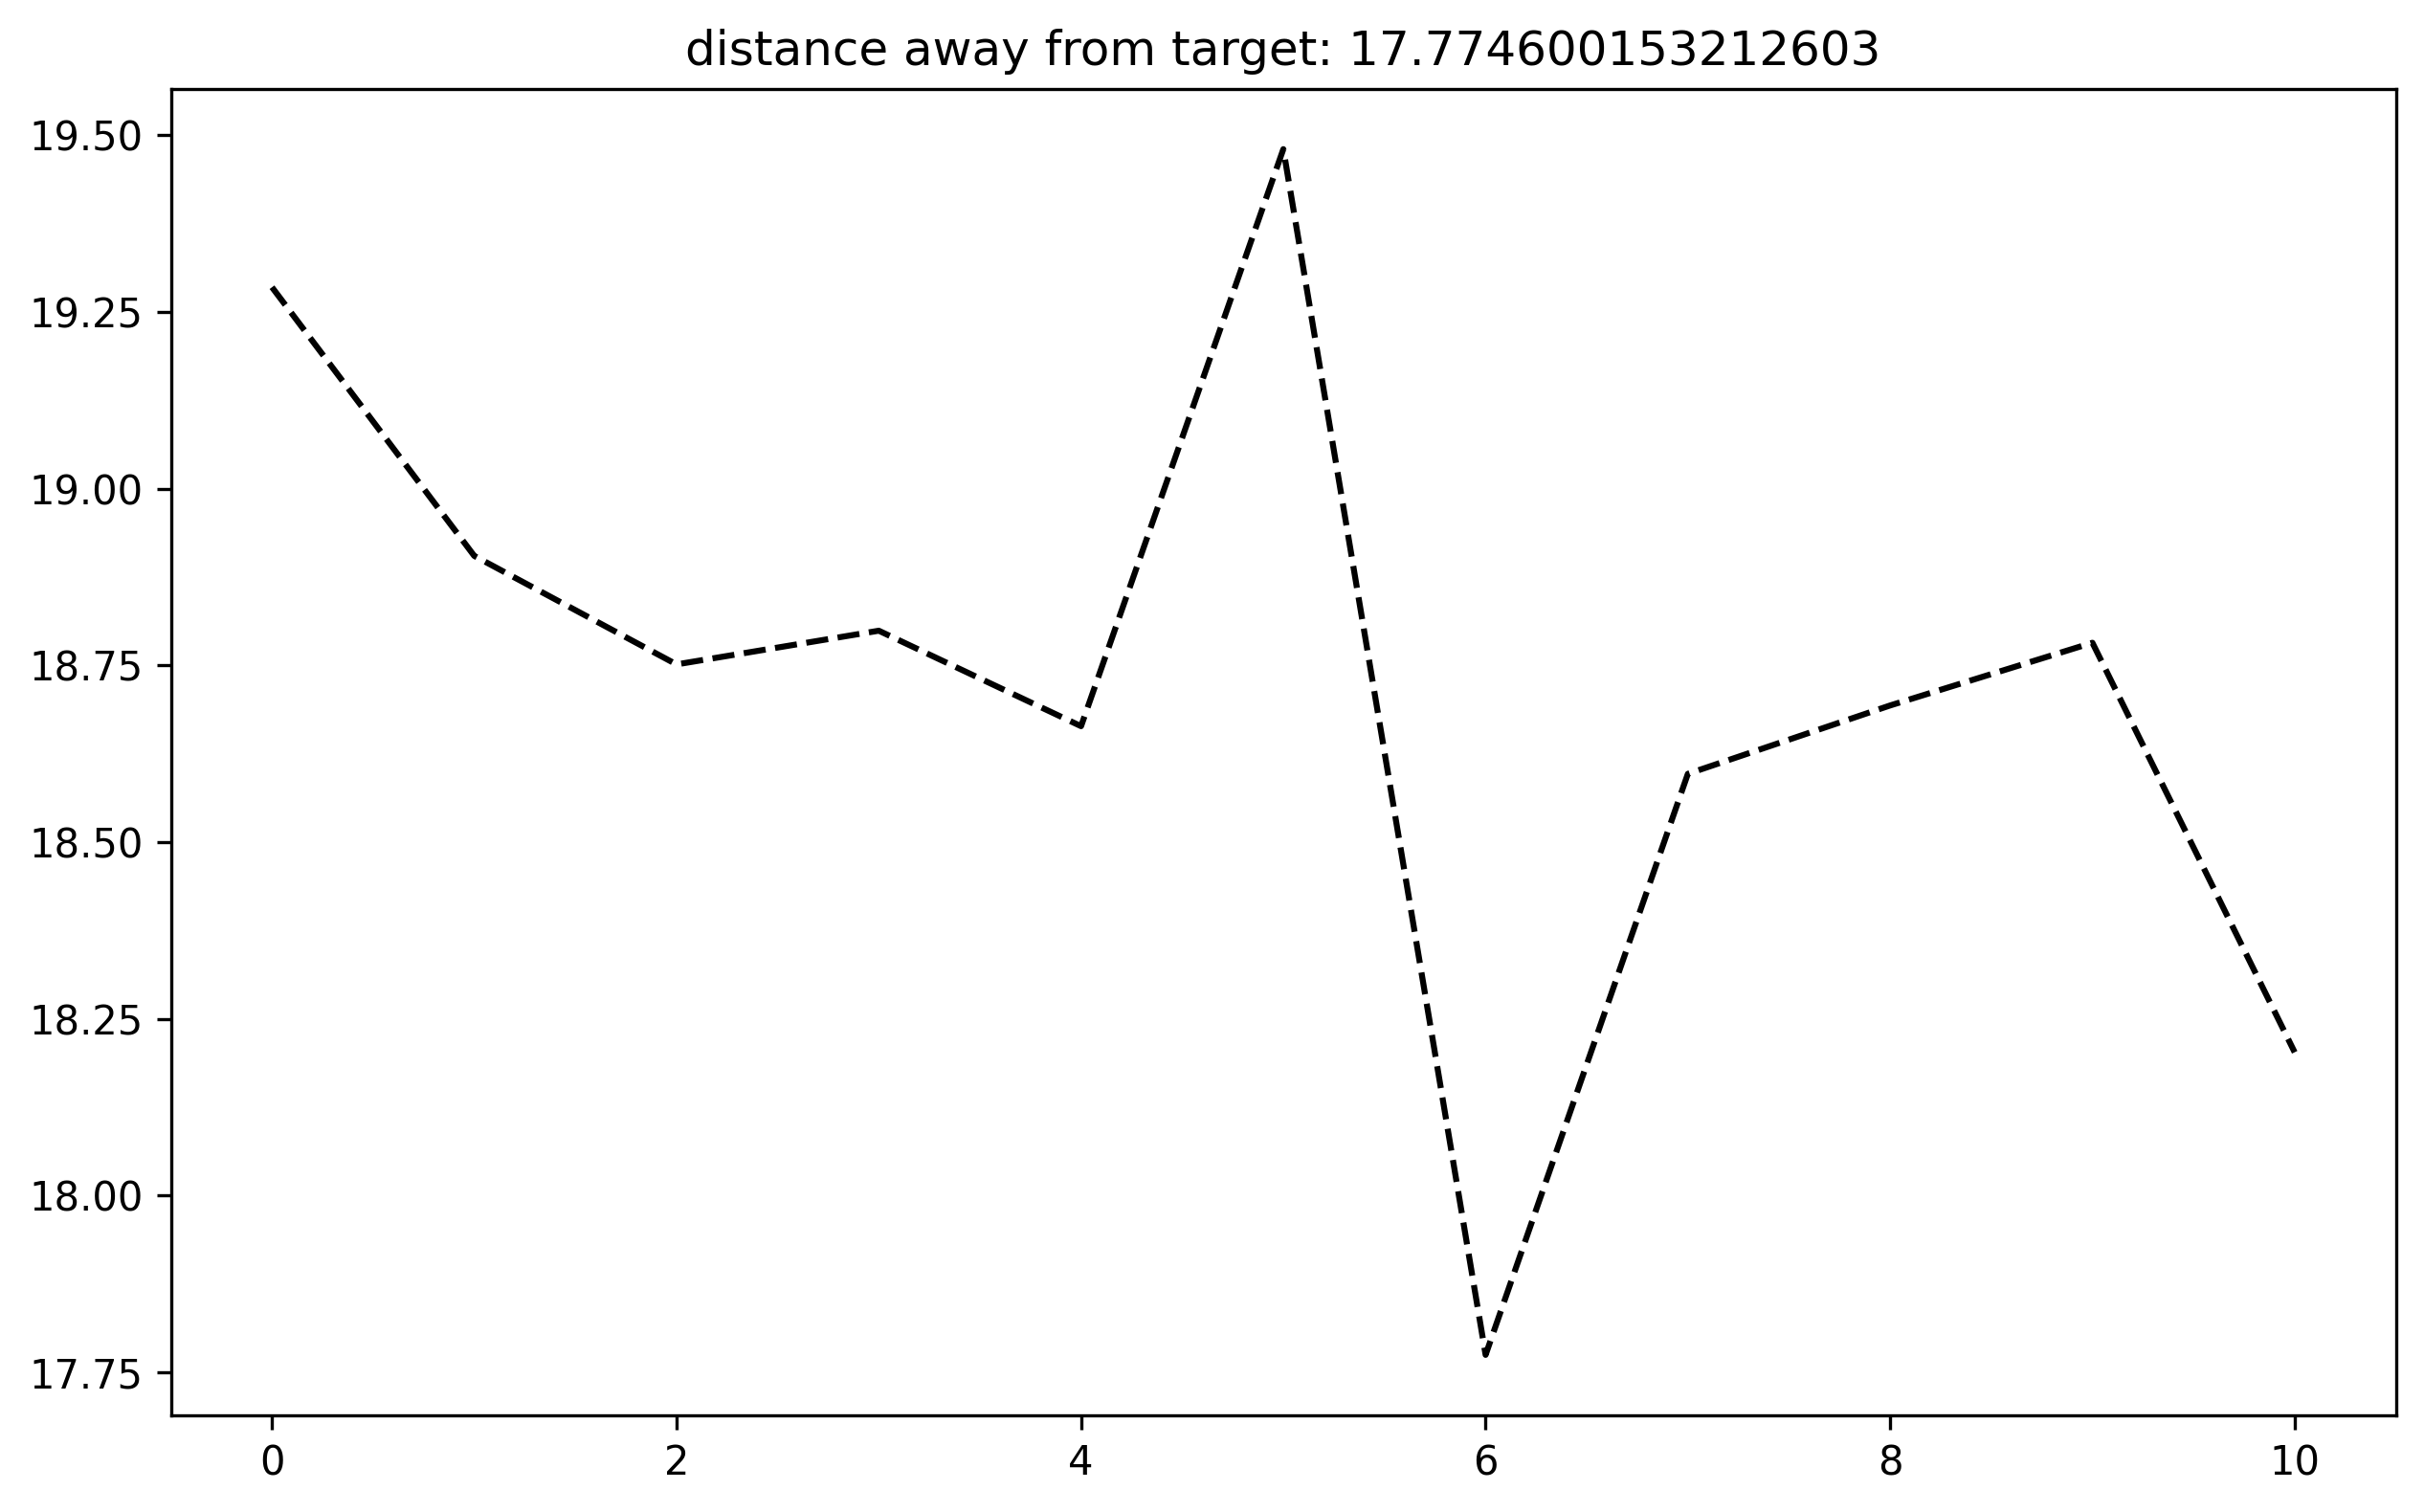
\includegraphics[width=\textwidth]{figures/filtered/mlp_custom_1.png}
		\caption*{AGT (Filtered): 1×1m}
	\end{minipage}
	\hfill
	\begin{minipage}{0.49\textwidth}
		\centering
		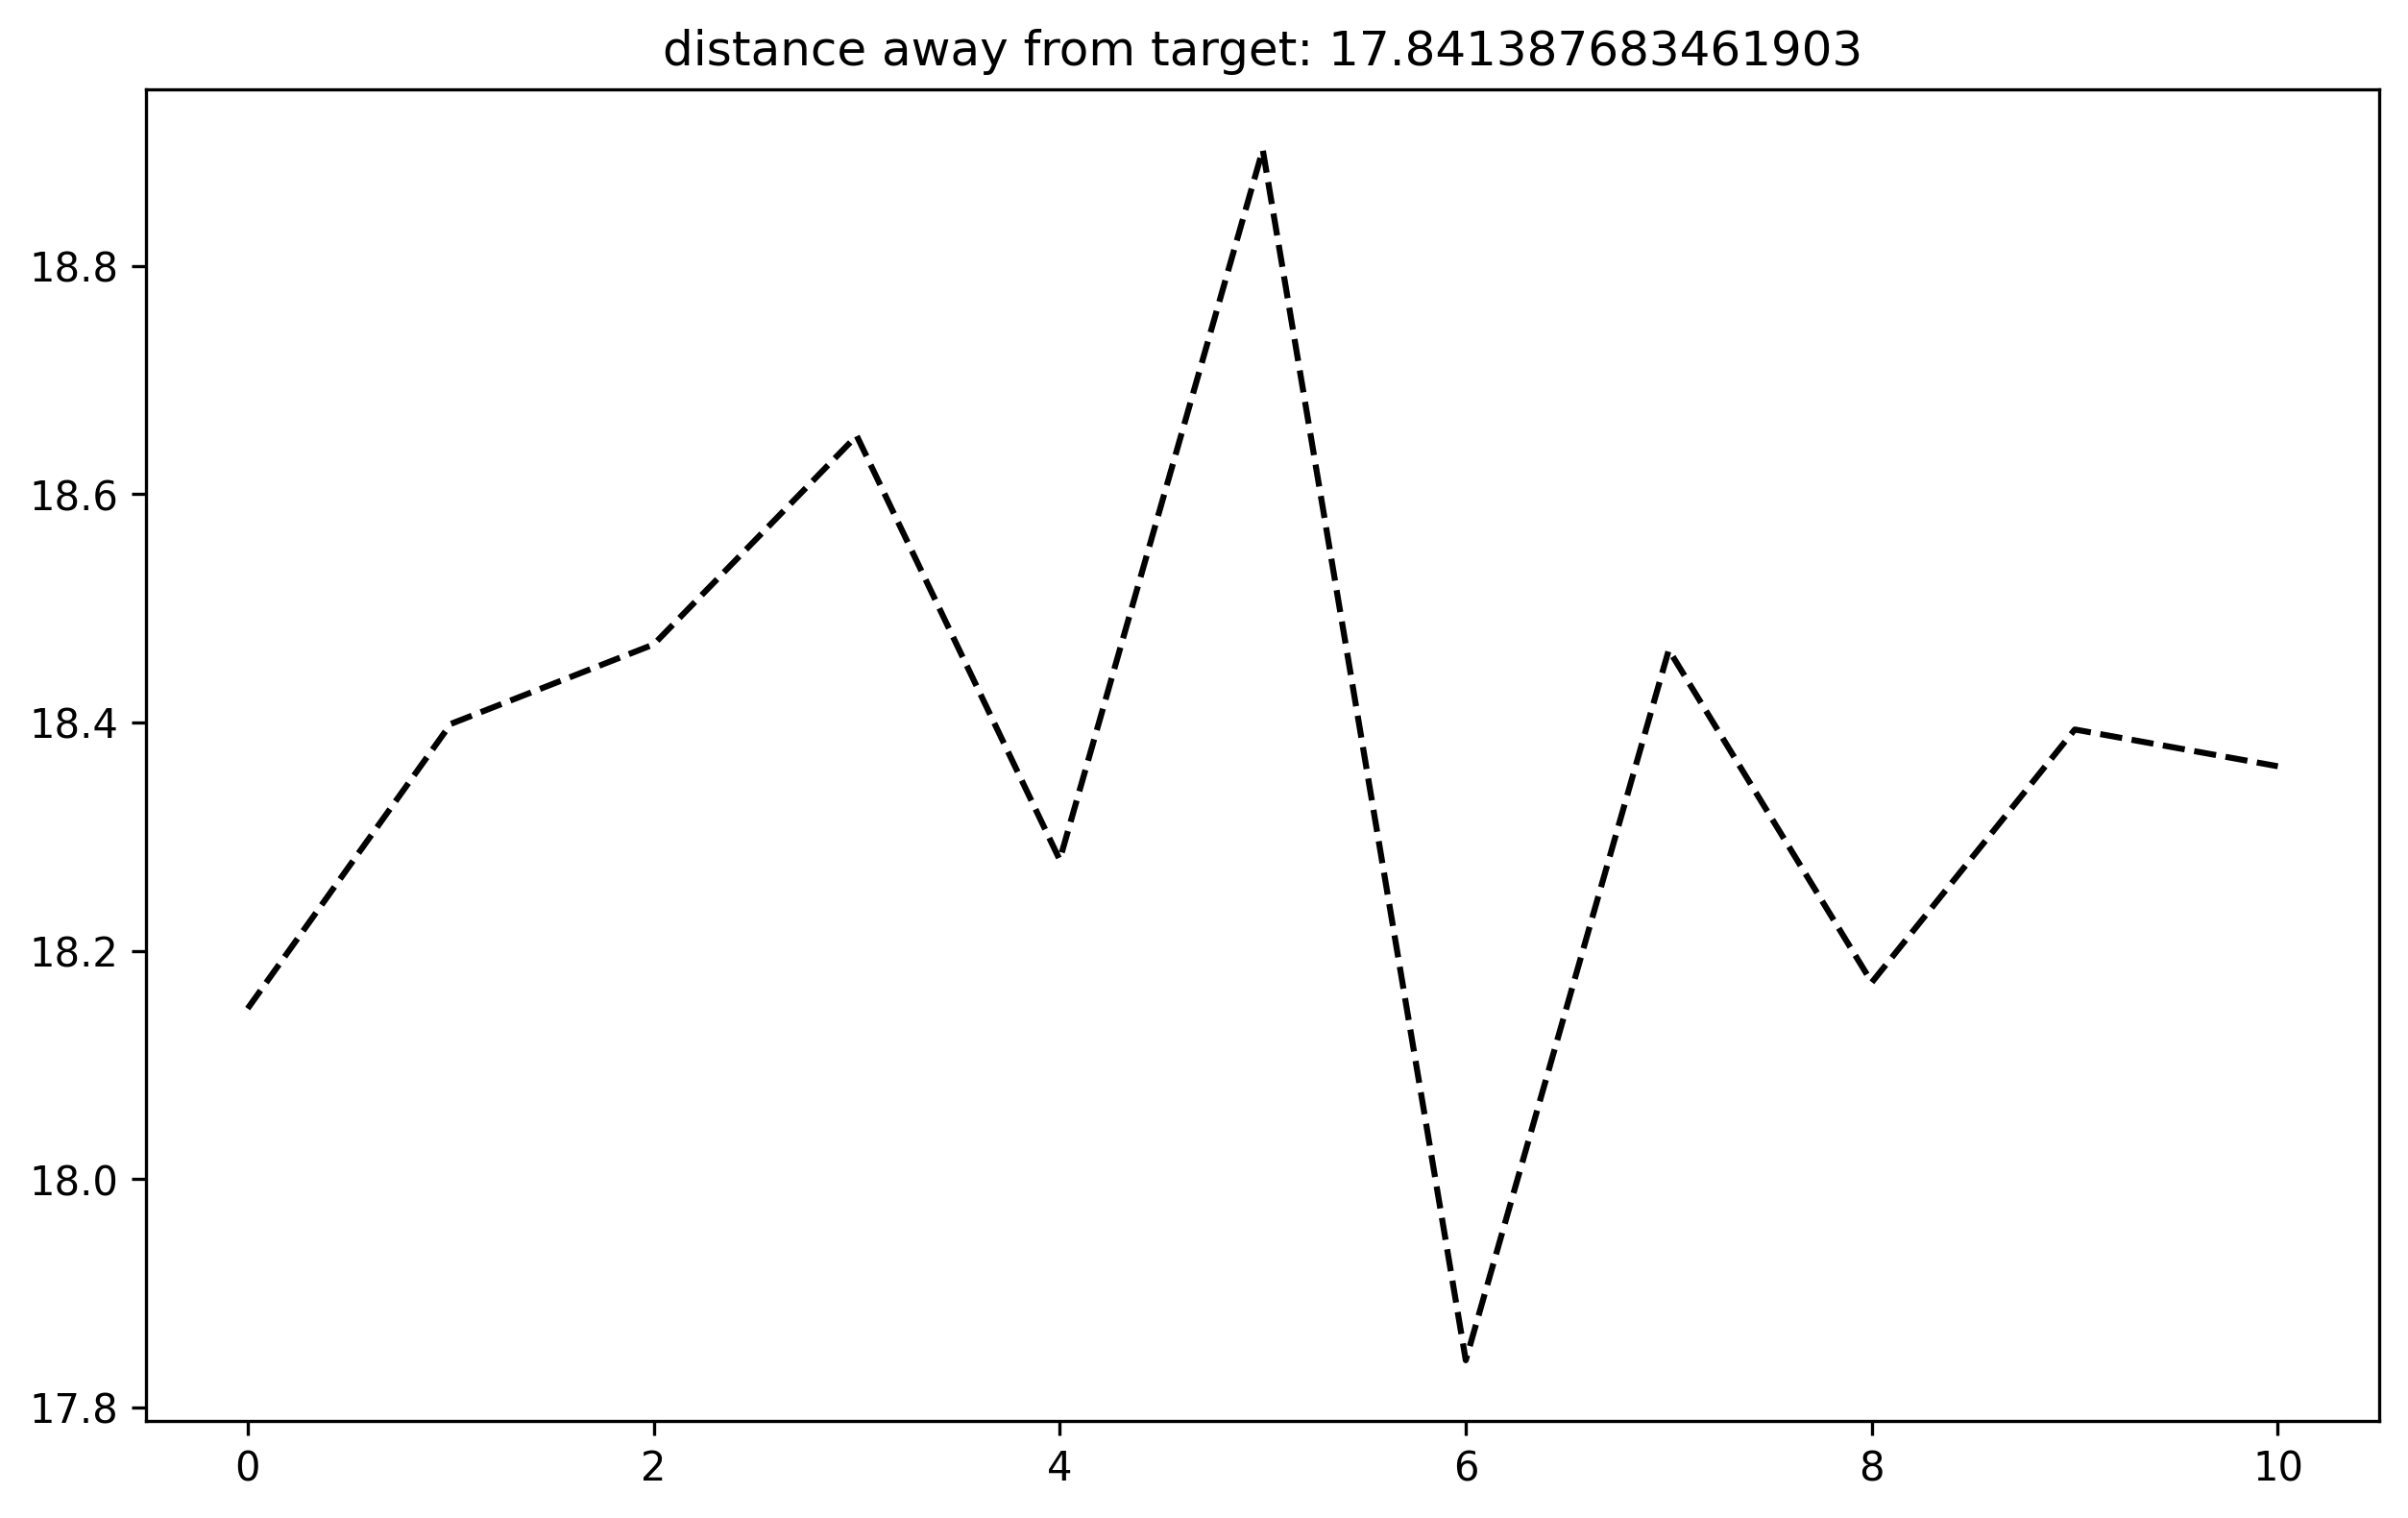
\includegraphics[width=\textwidth]{figures/unfiltered/mlp_custom_1.png}
		\caption*{AGT (Unfiltered): 1×1m}
	\end{minipage}
\end{figure}

\begin{figure}[H]
	\centering
	\begin{minipage}{0.49\textwidth}
		\centering
		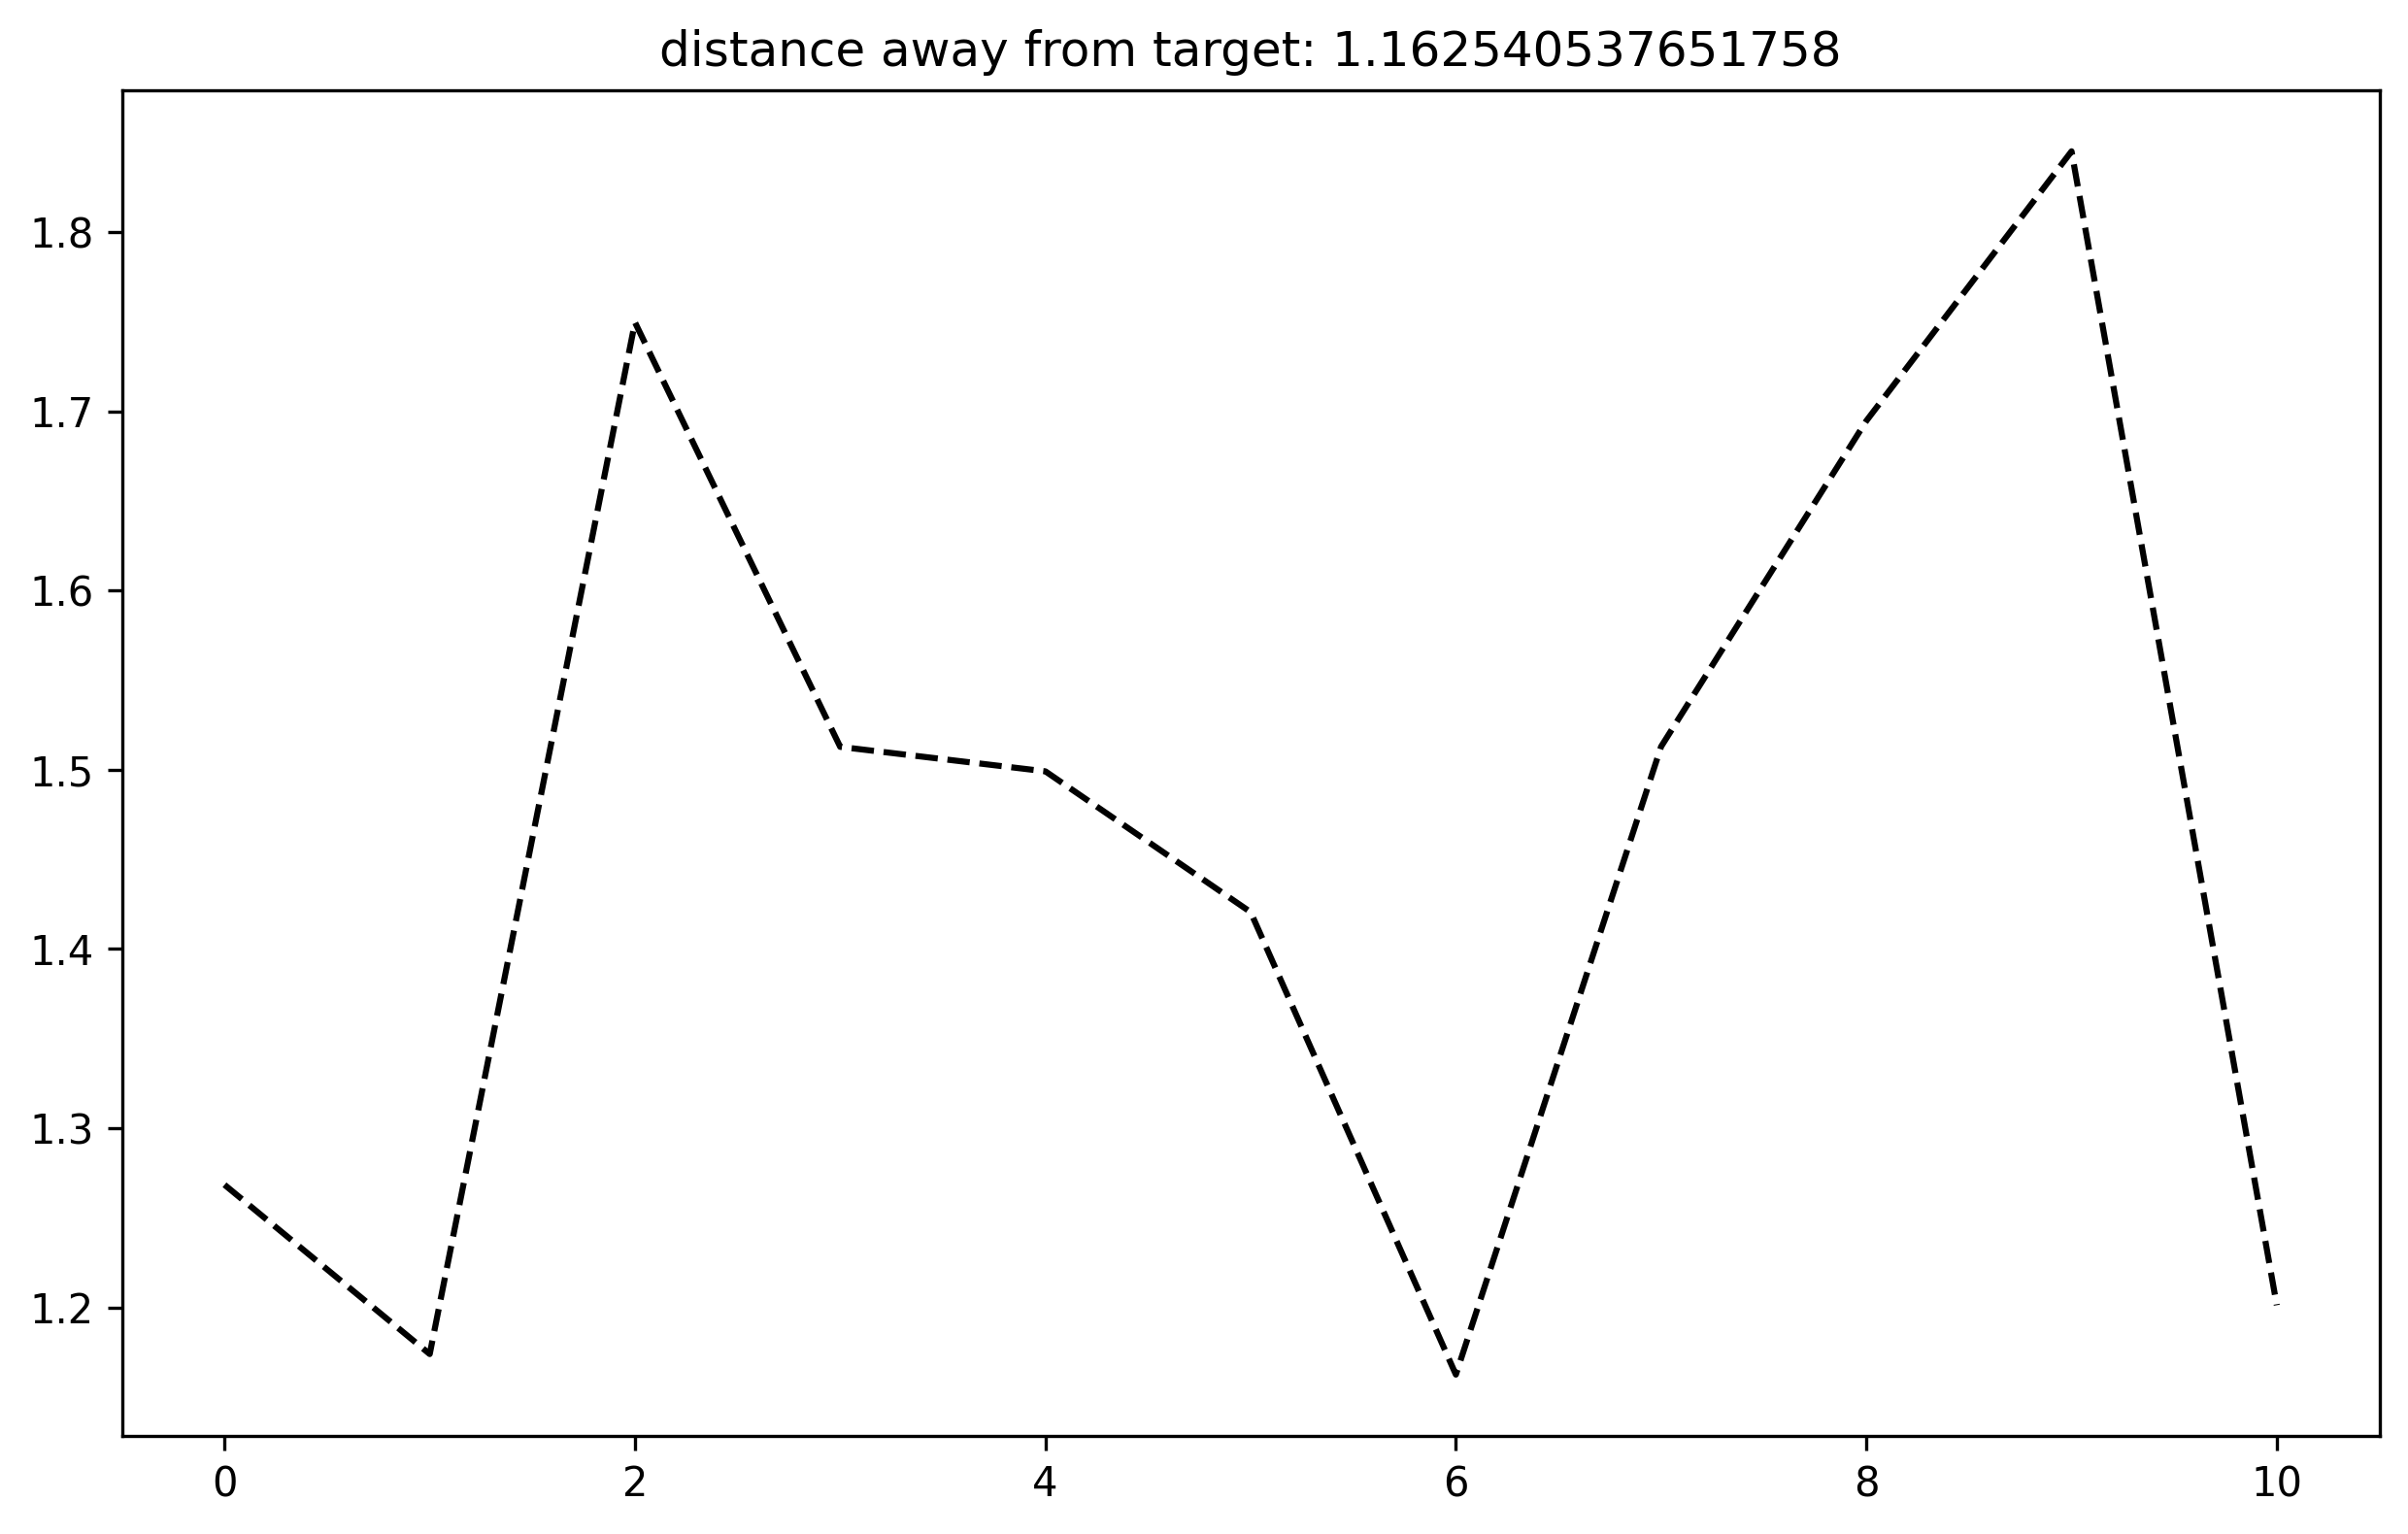
\includegraphics[width=\textwidth]{figures/filtered/mlp_custom_7.png}
		\caption*{AGT (Filtered): 7×7m}
	\end{minipage}
	\hfill
	\begin{minipage}{0.49\textwidth}
		\centering
		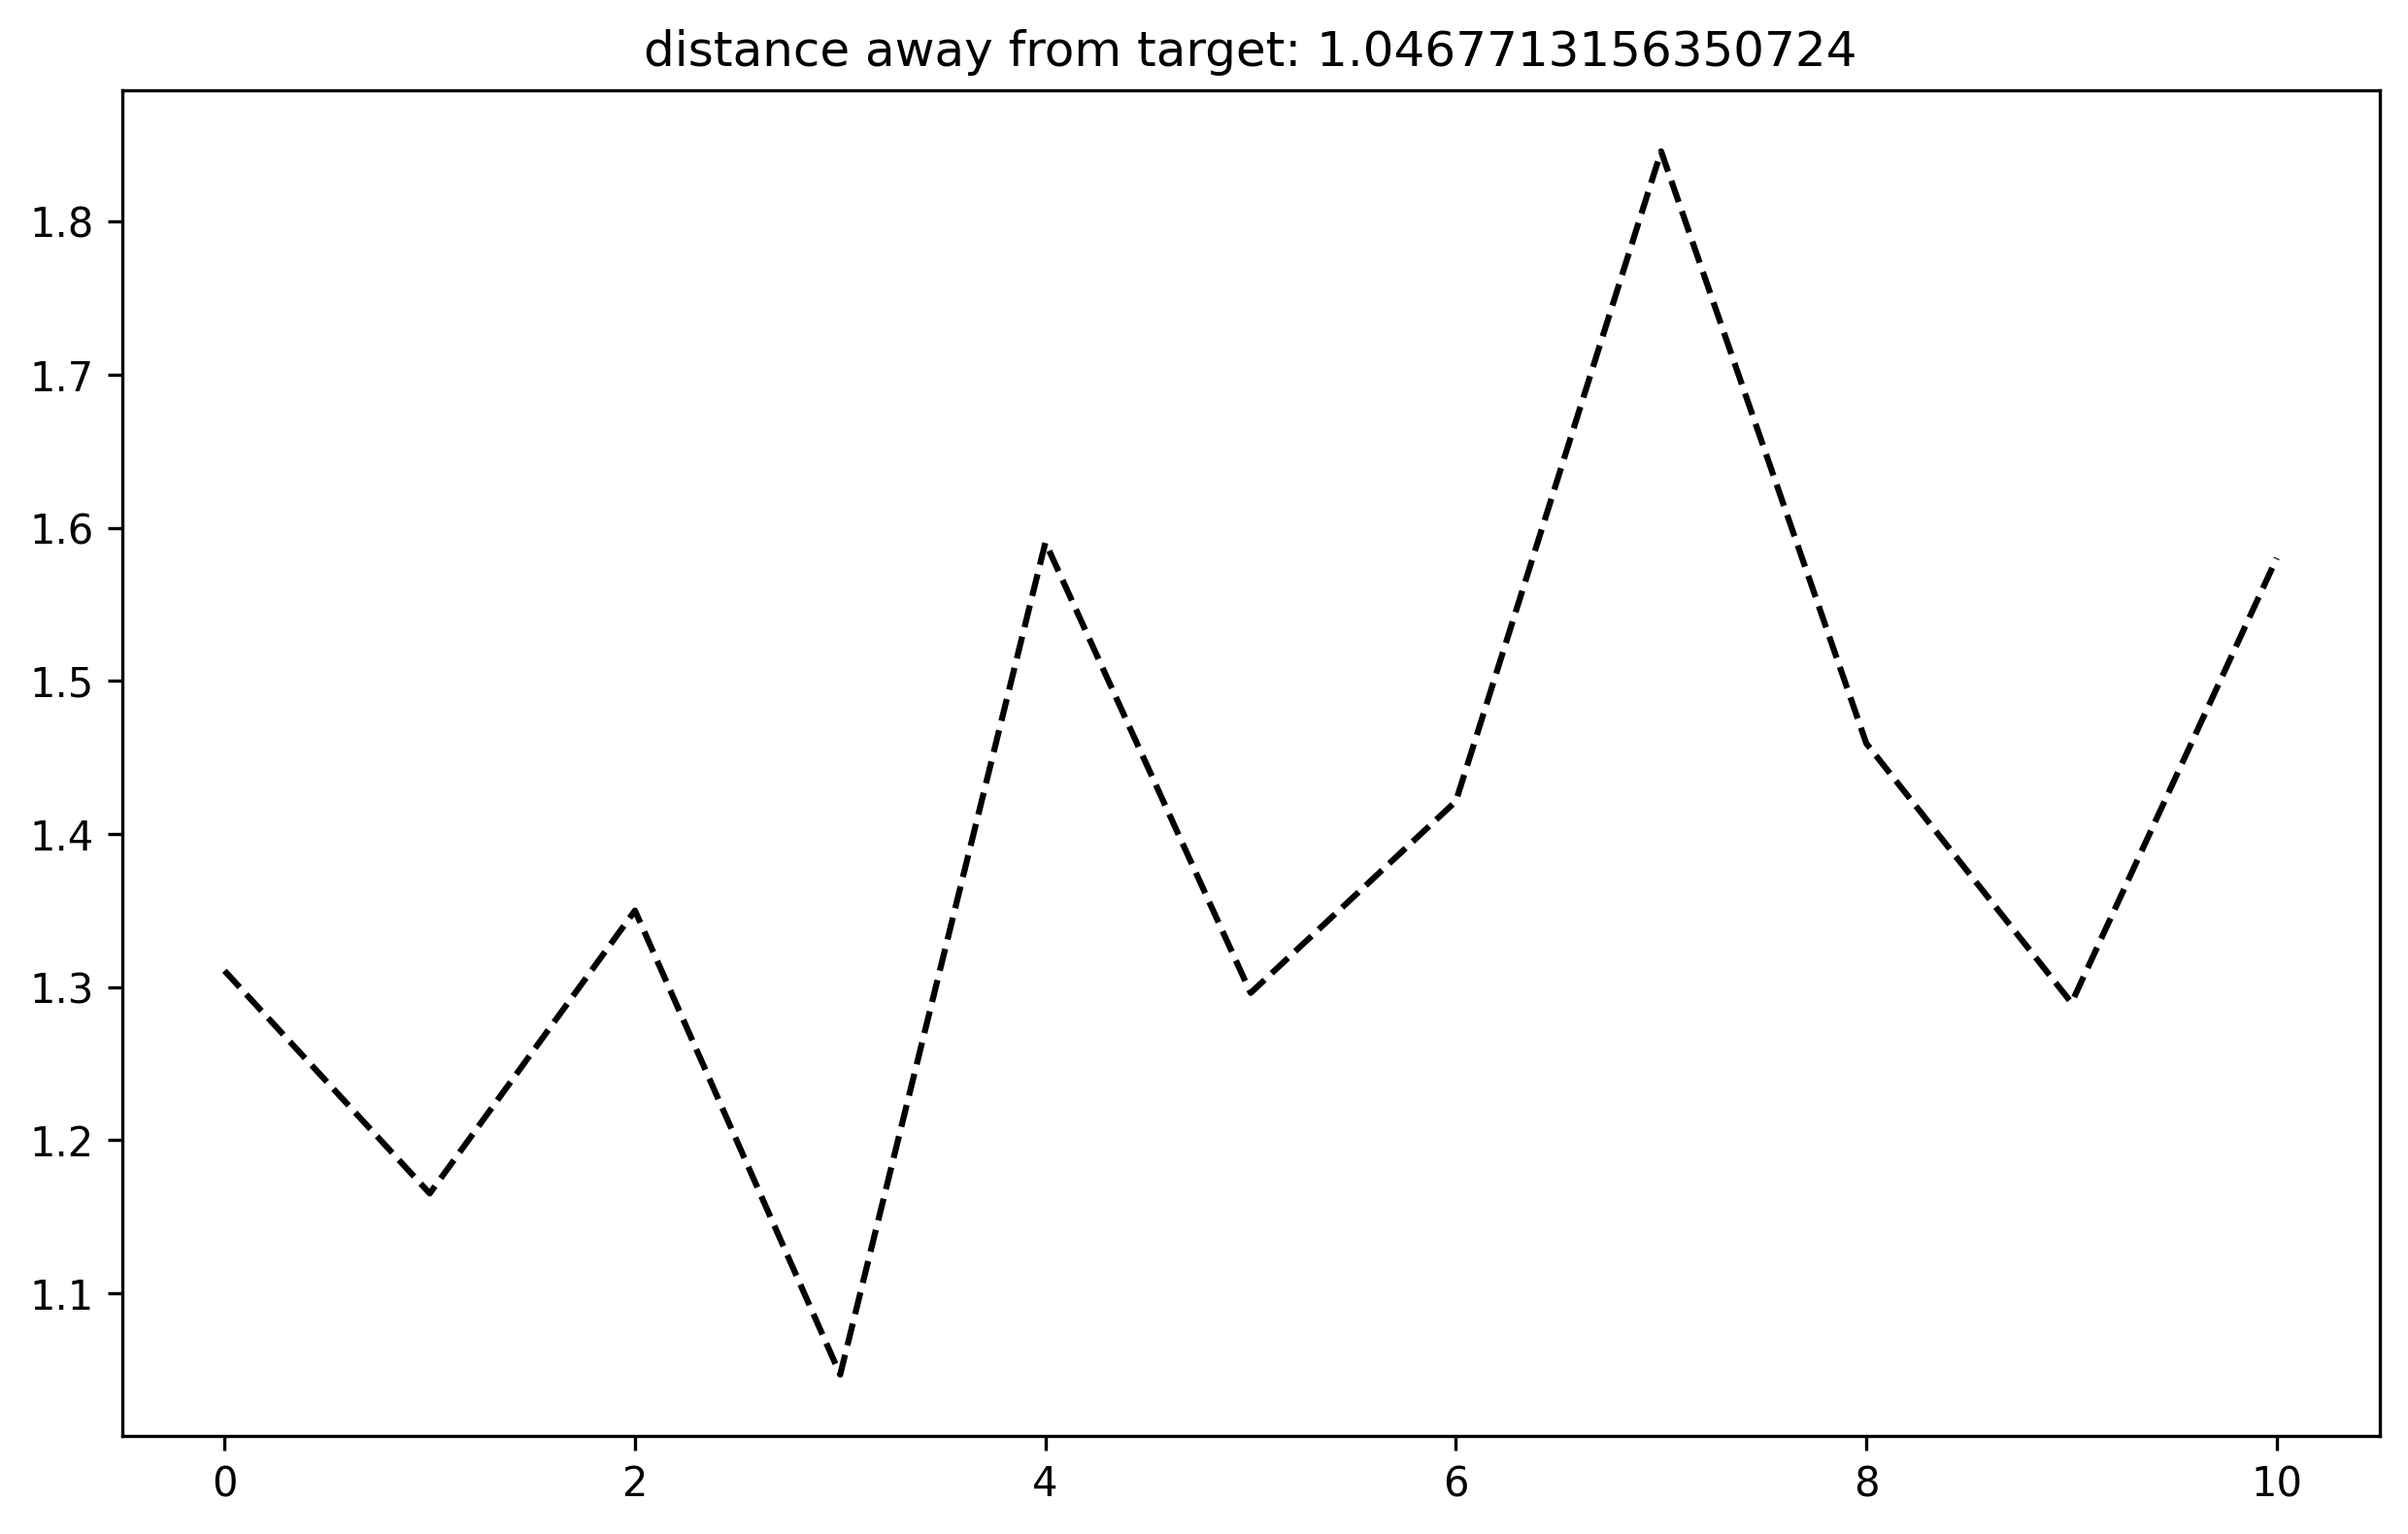
\includegraphics[width=\textwidth]{figures/unfiltered/mlp_custom_7.png}
		\caption*{AGT (Unfiltered): 7×7m}
	\end{minipage}
\end{figure}

\begin{figure}[H]
	\centering
	\begin{minipage}{0.49\textwidth}
		\centering
		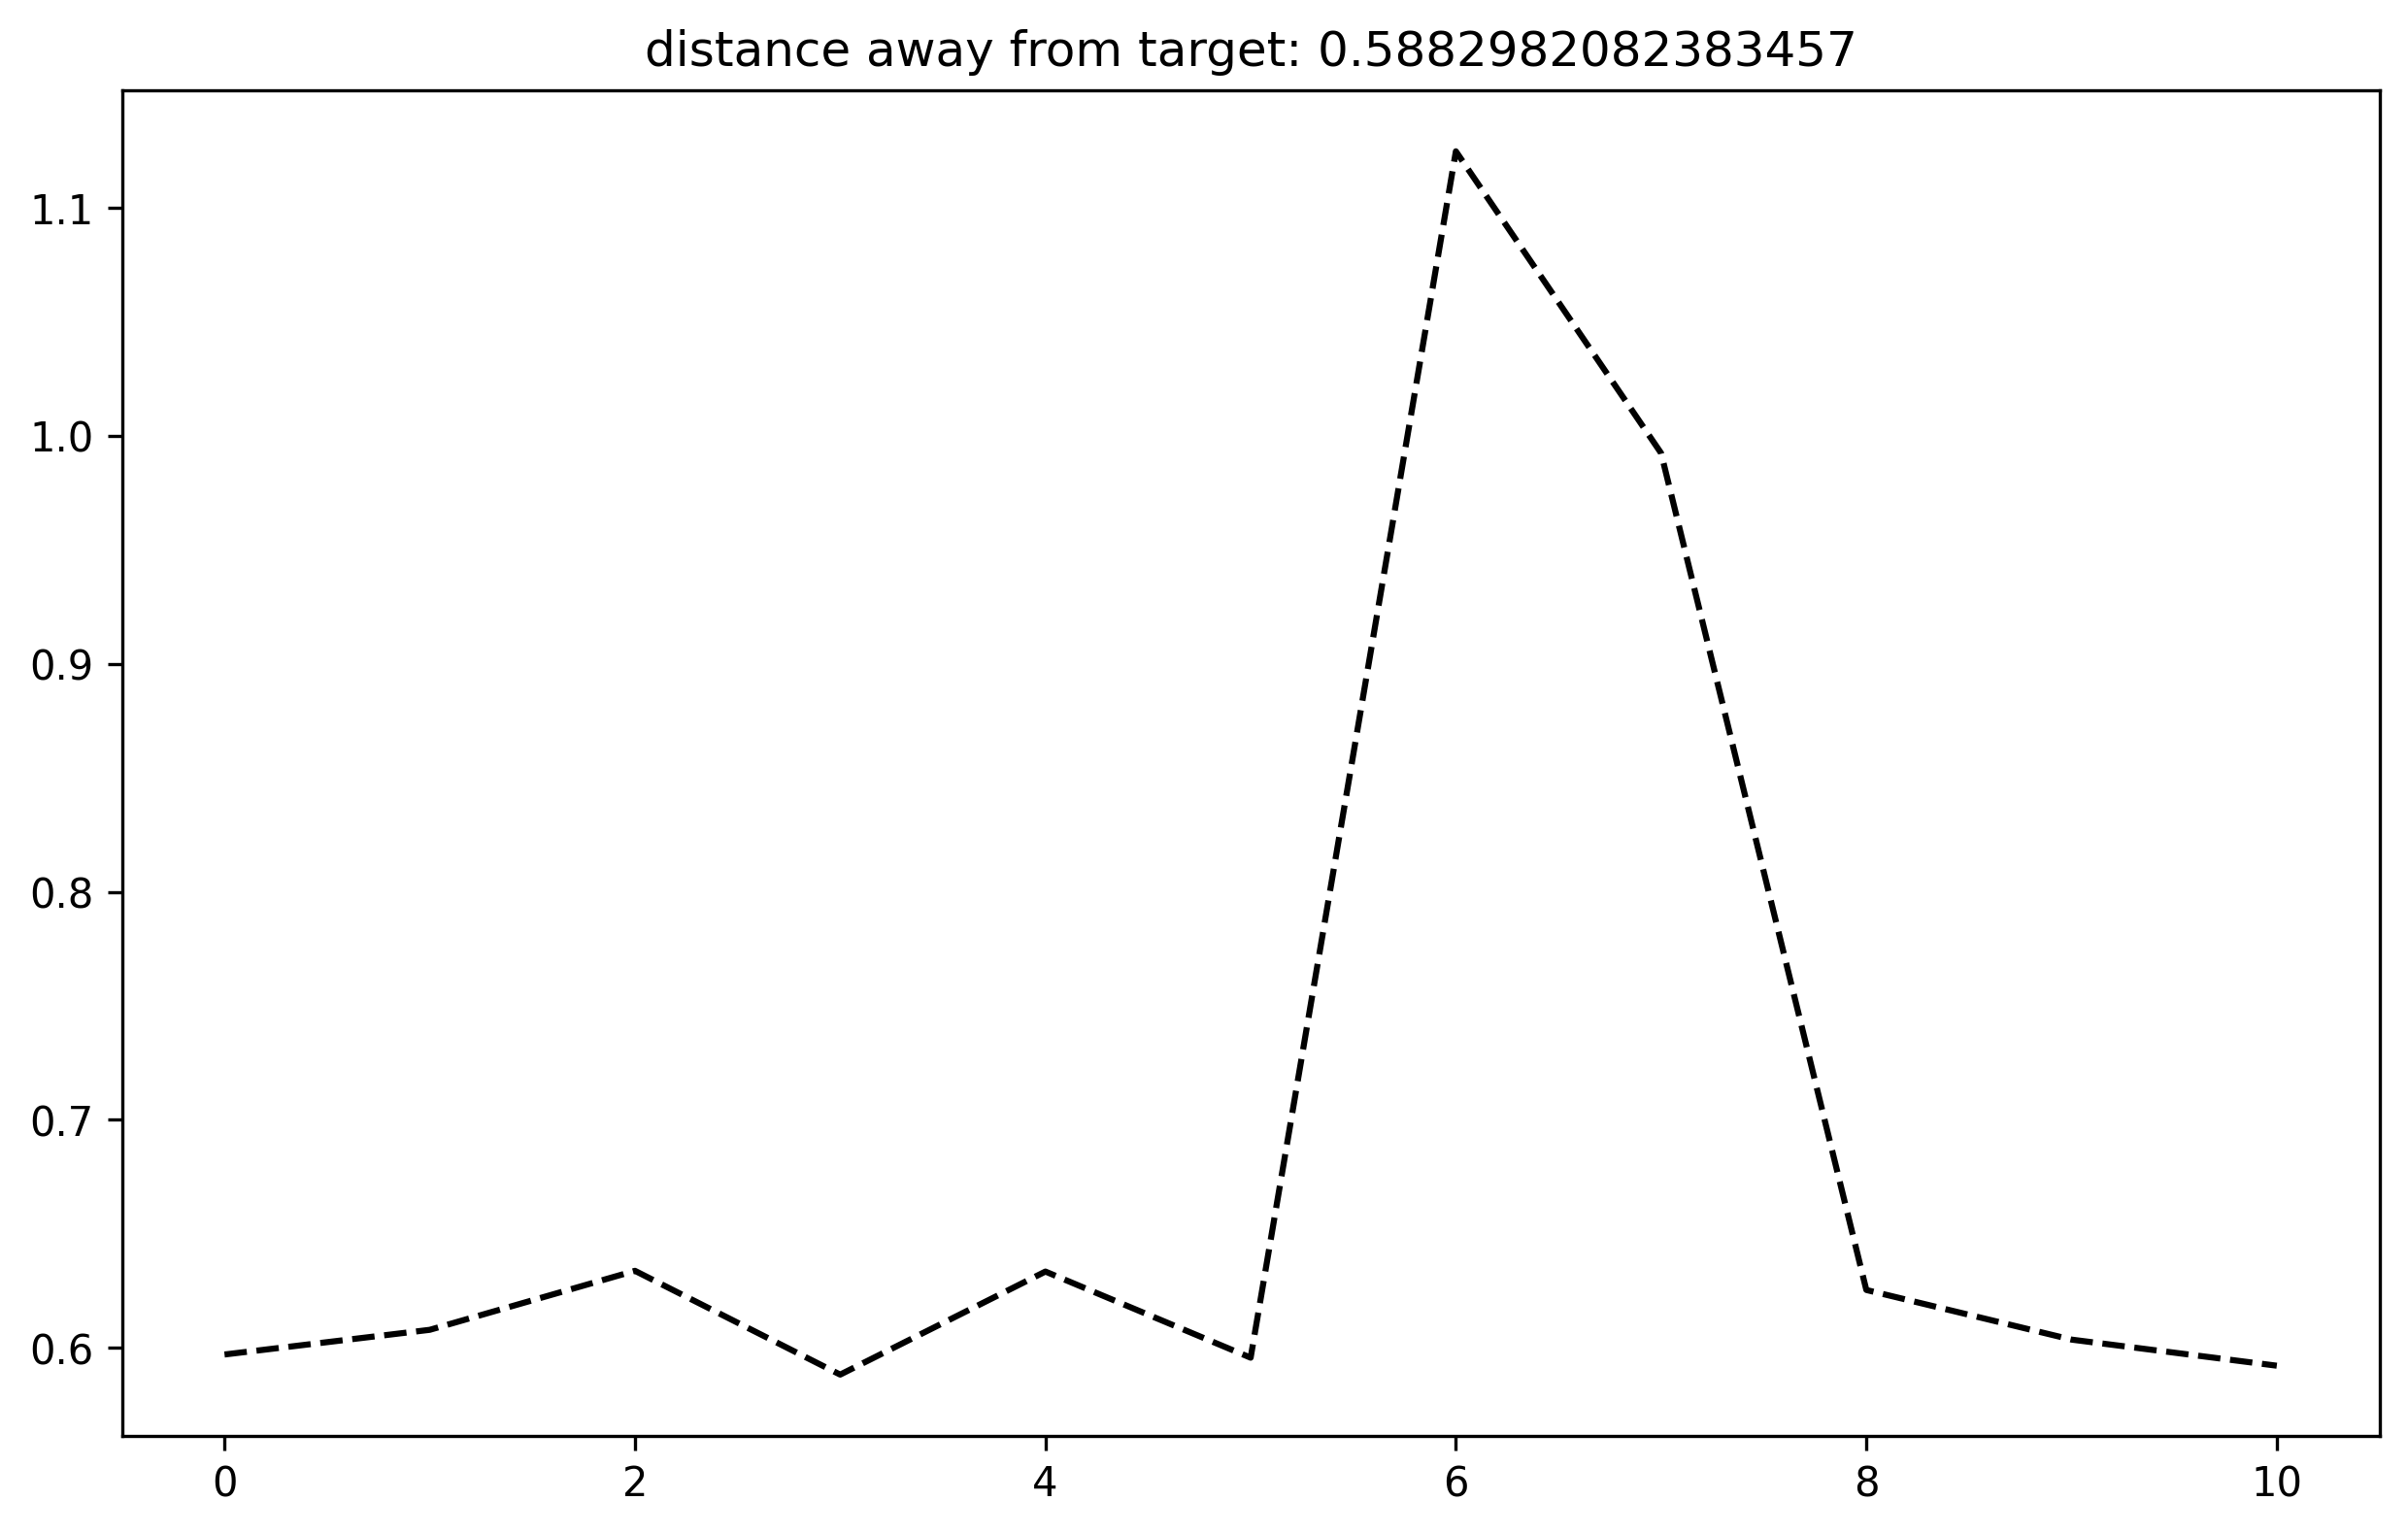
\includegraphics[width=\textwidth]{figures/filtered/mlp_custom_15.png}
		\caption*{AGT (Filtered): 15×15m}
	\end{minipage}
	\hfill
	\begin{minipage}{0.49\textwidth}
		\centering
		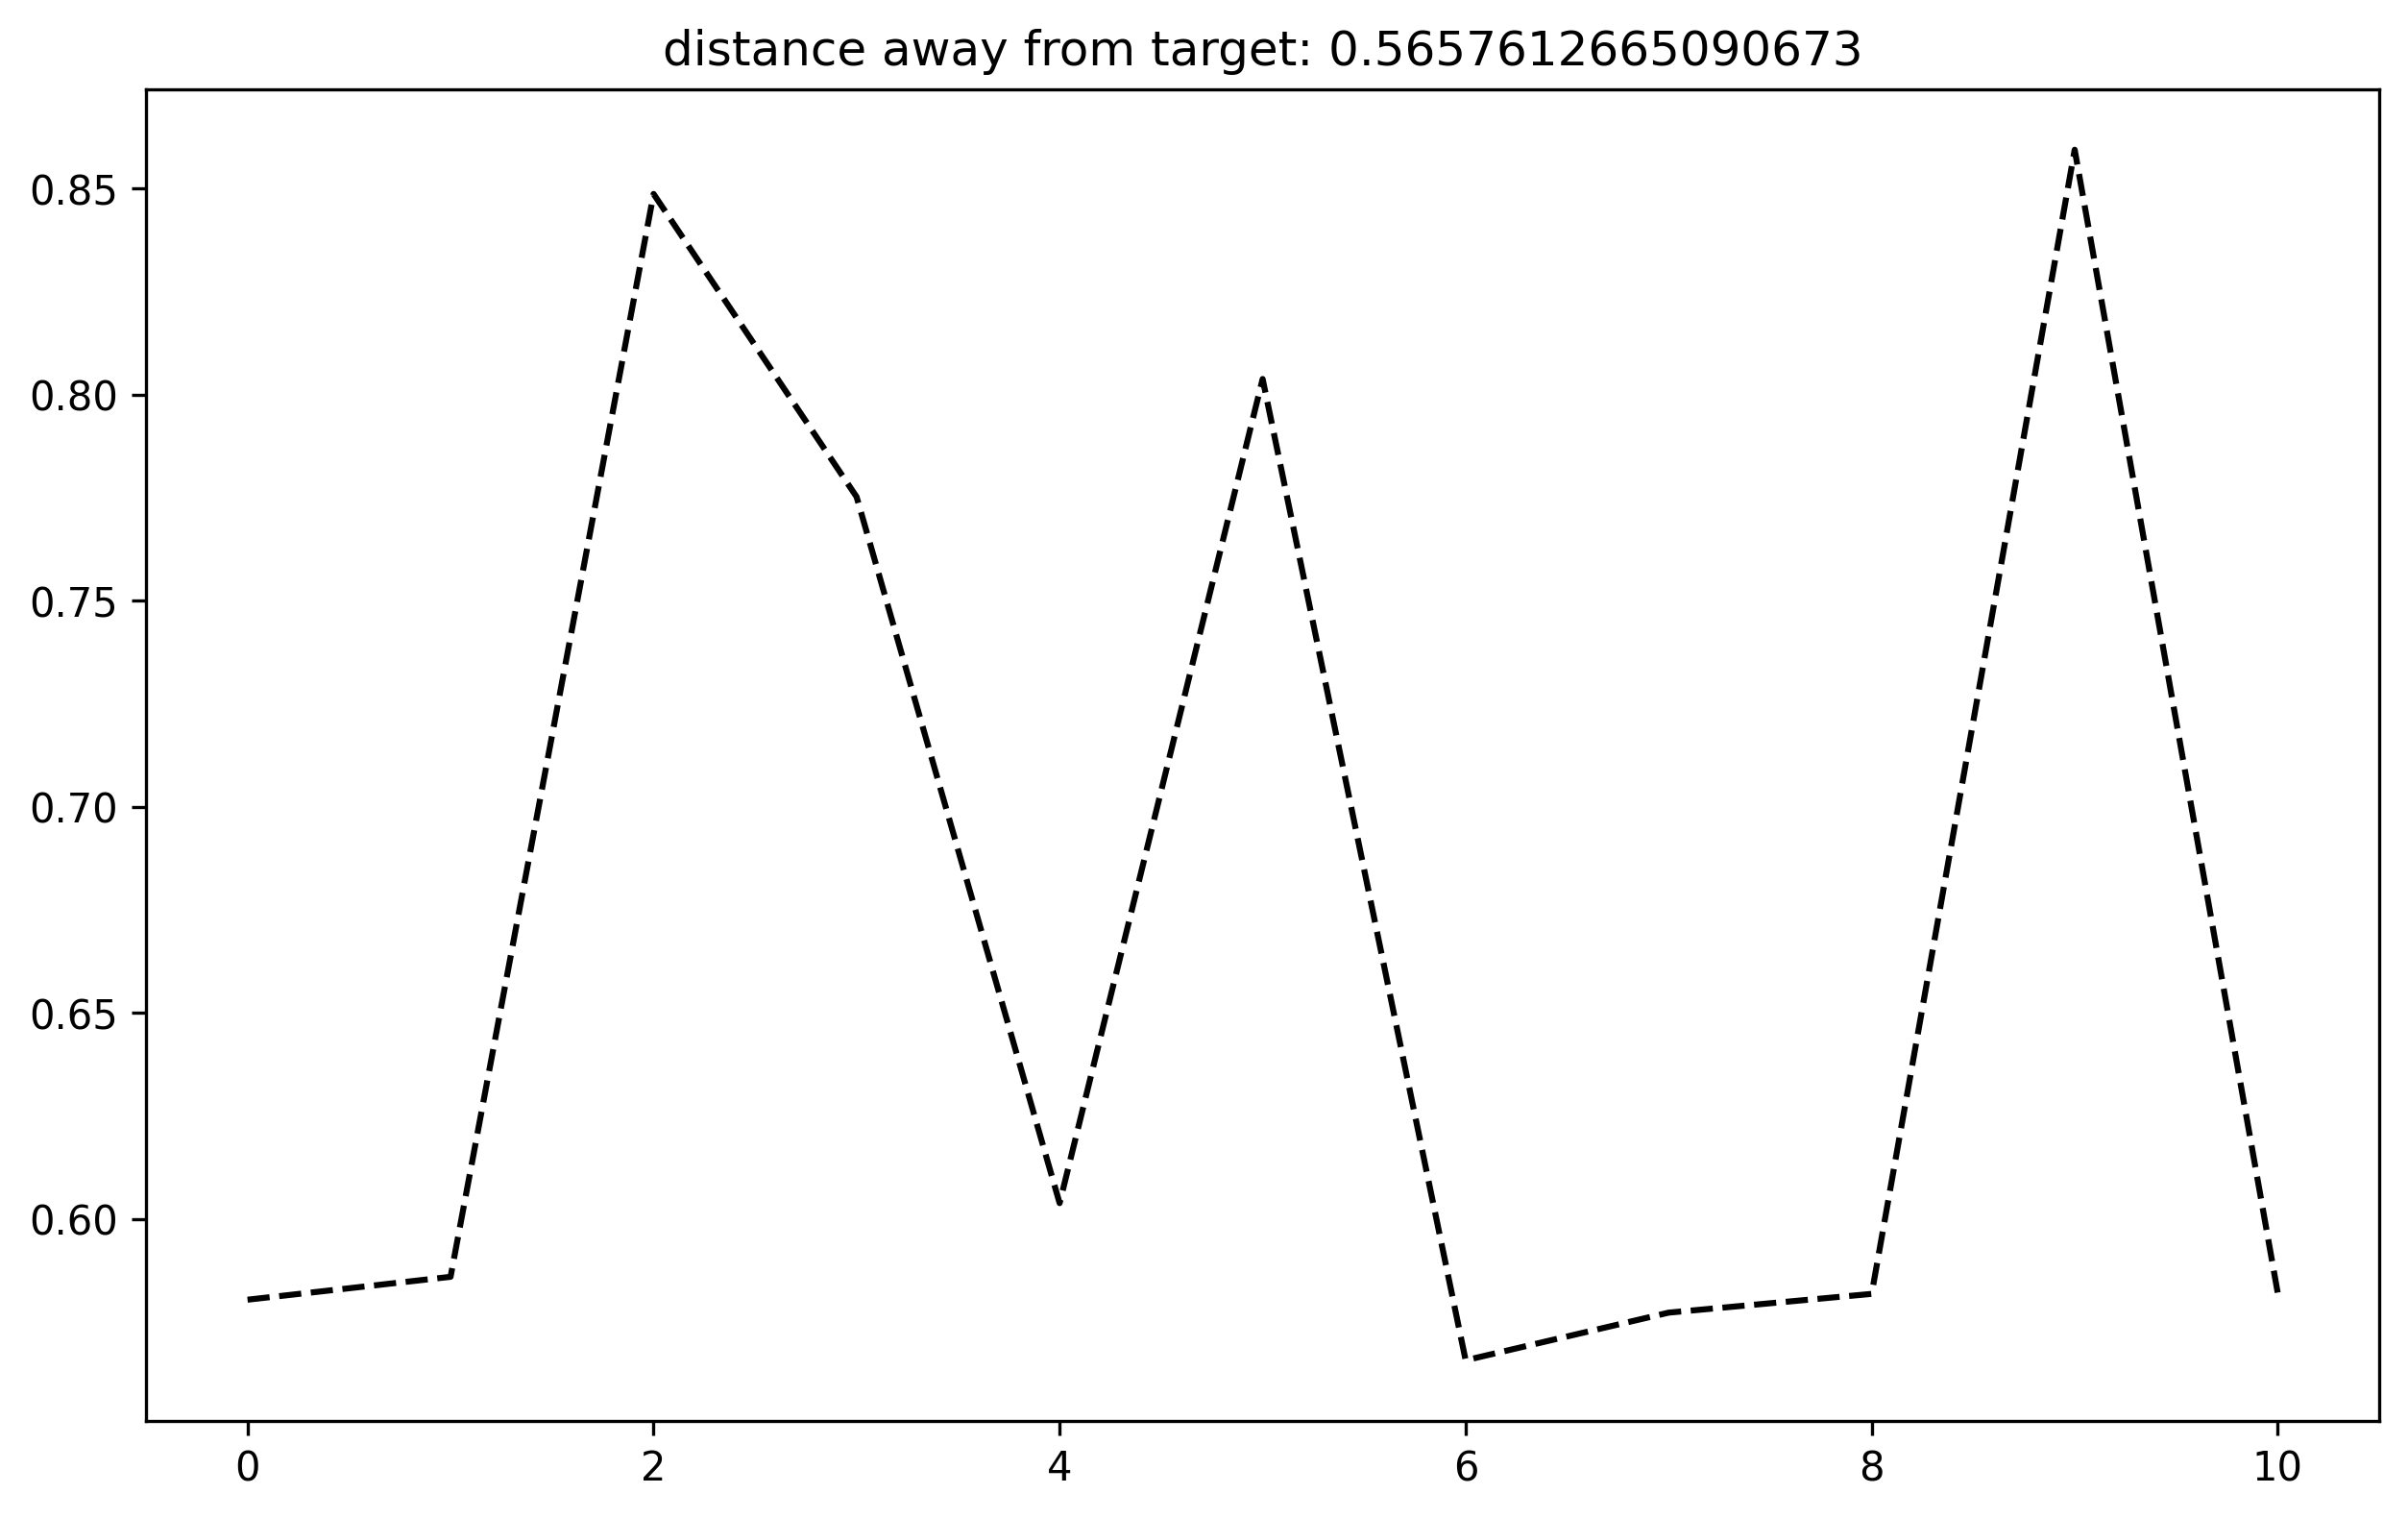
\includegraphics[width=\textwidth]{figures/unfiltered/mlp_custom_15.png}
		\caption*{AGT (Unfiltered): 15×15m}
	\end{minipage}
\end{figure}

\clearpage

\subsection*{SVM}

\begin{figure}[H]
	\centering
	\begin{minipage}{0.49\textwidth}
		\centering
		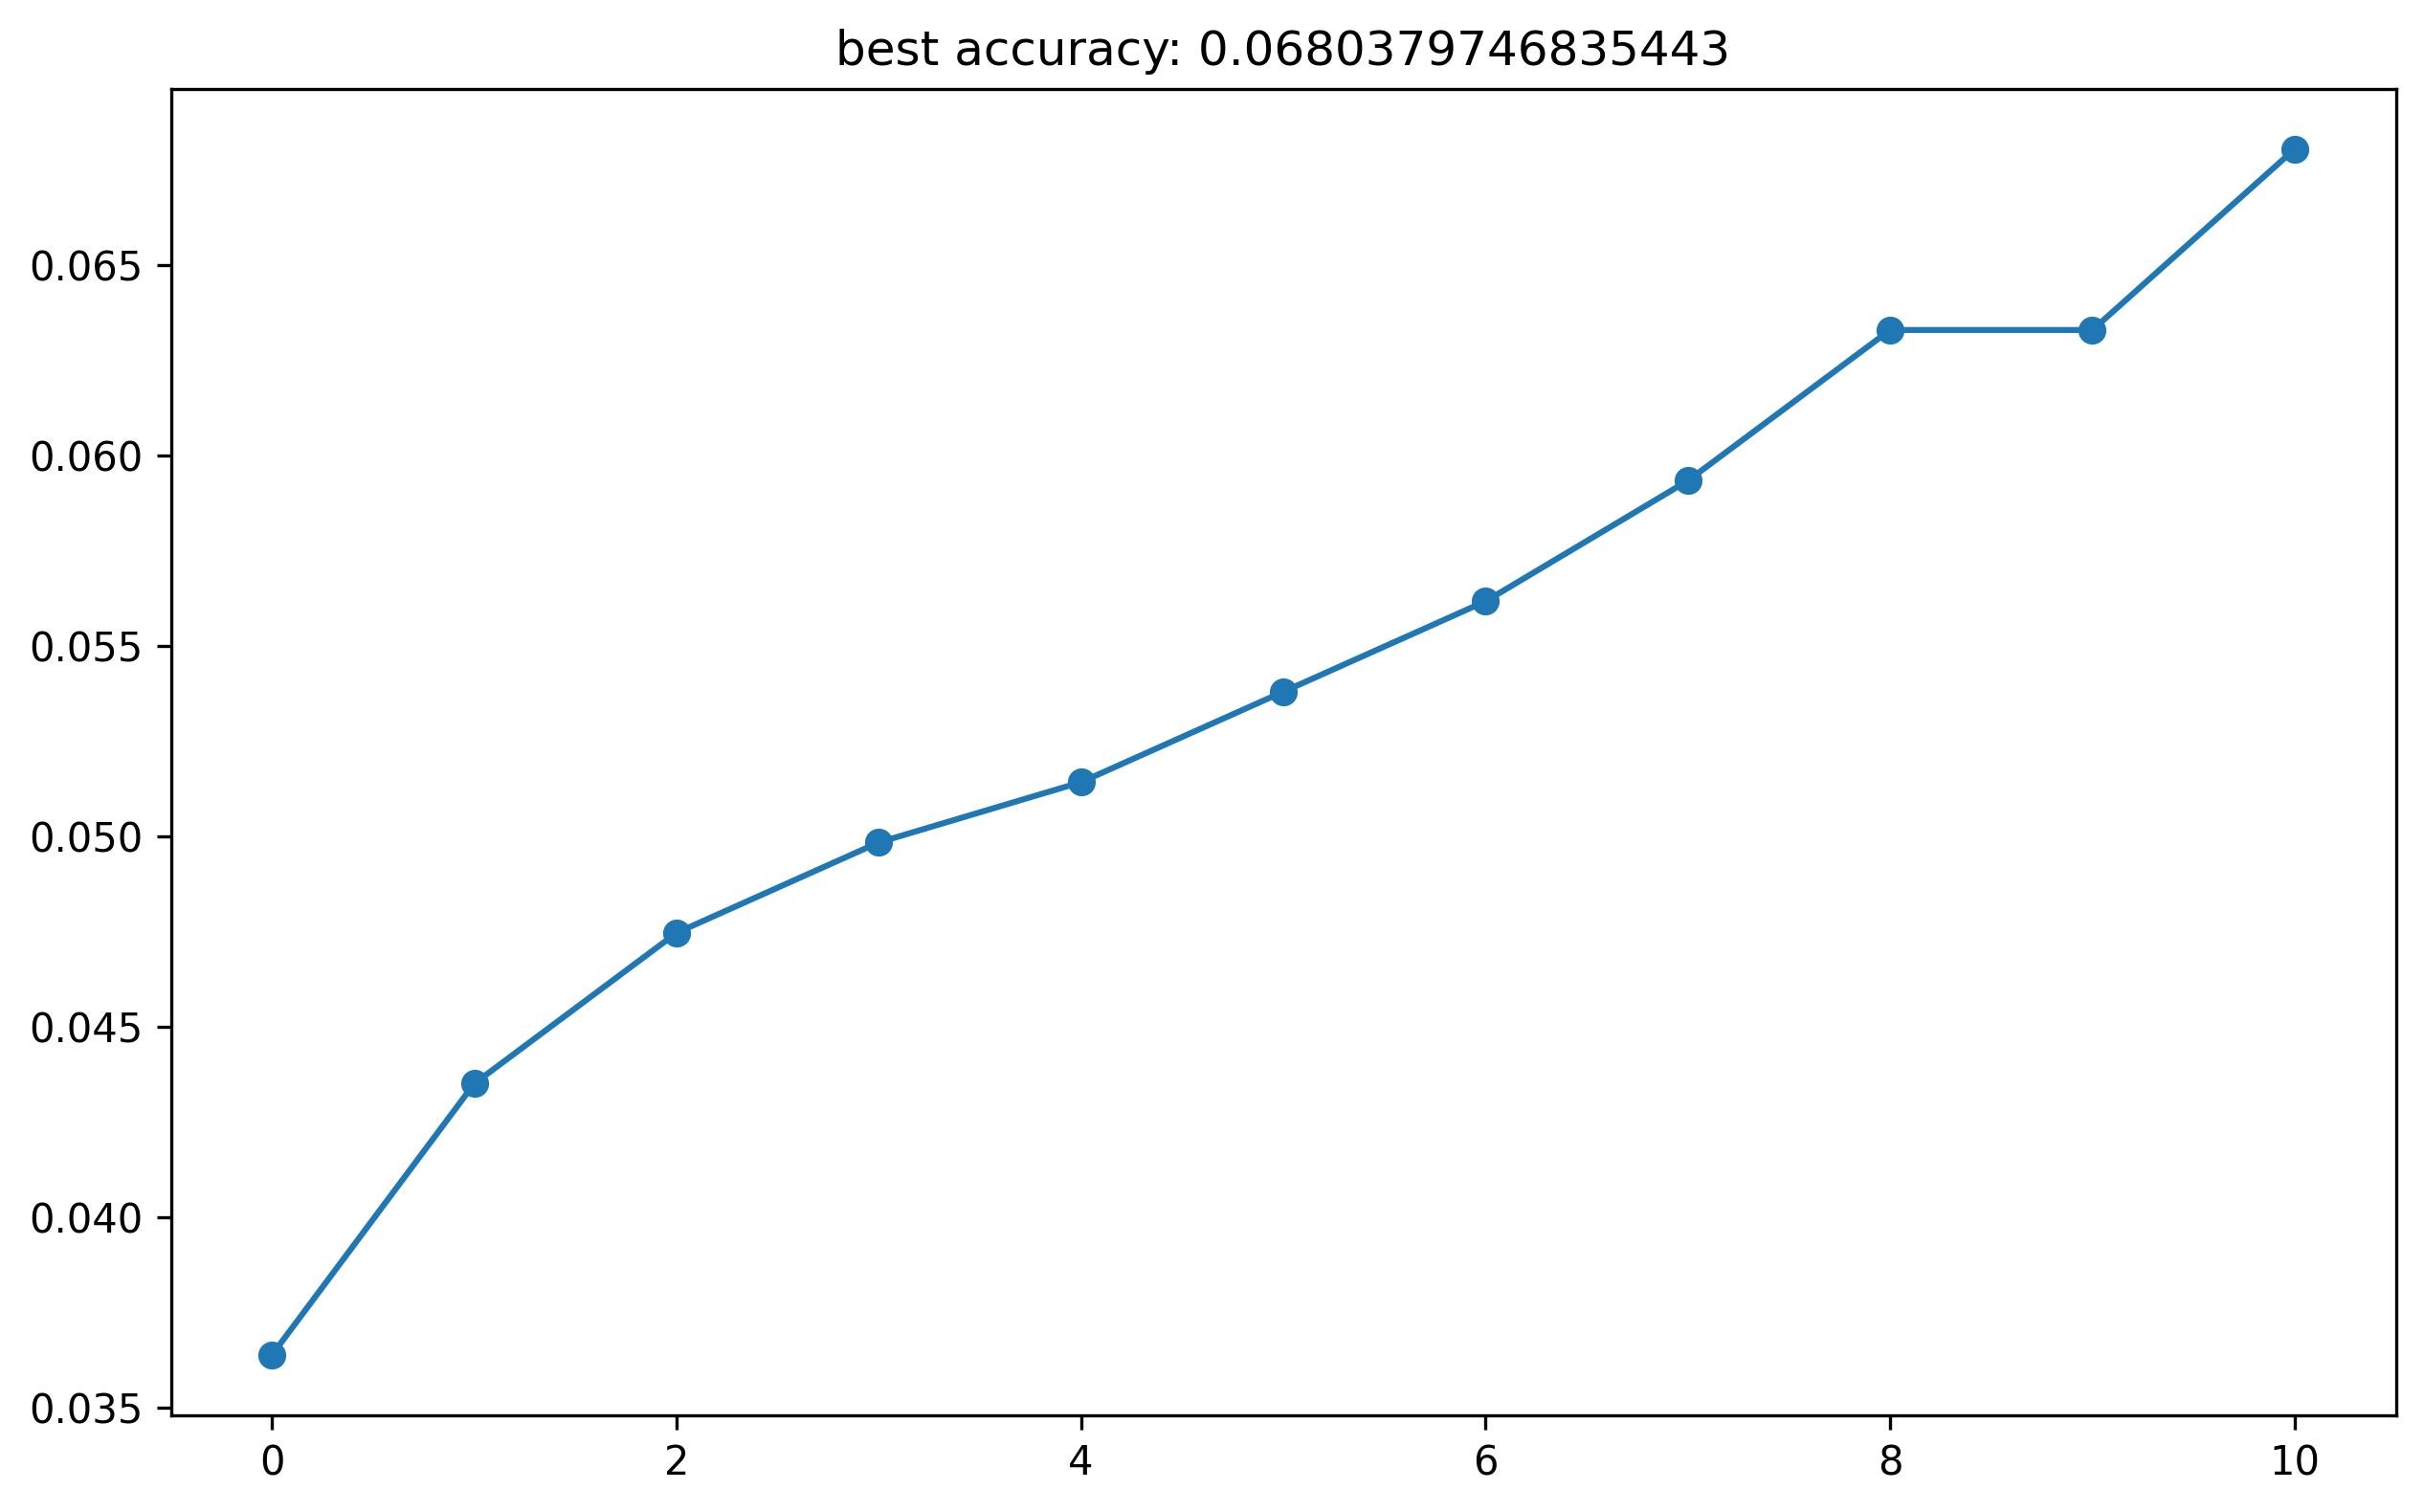
\includegraphics[width=\textwidth]{figures/filtered/svm_acc_1.png}
		\caption*{Accuracy (Filtered): 1×1m}
	\end{minipage}
	\hfill
	\begin{minipage}{0.49\textwidth}
		\centering
		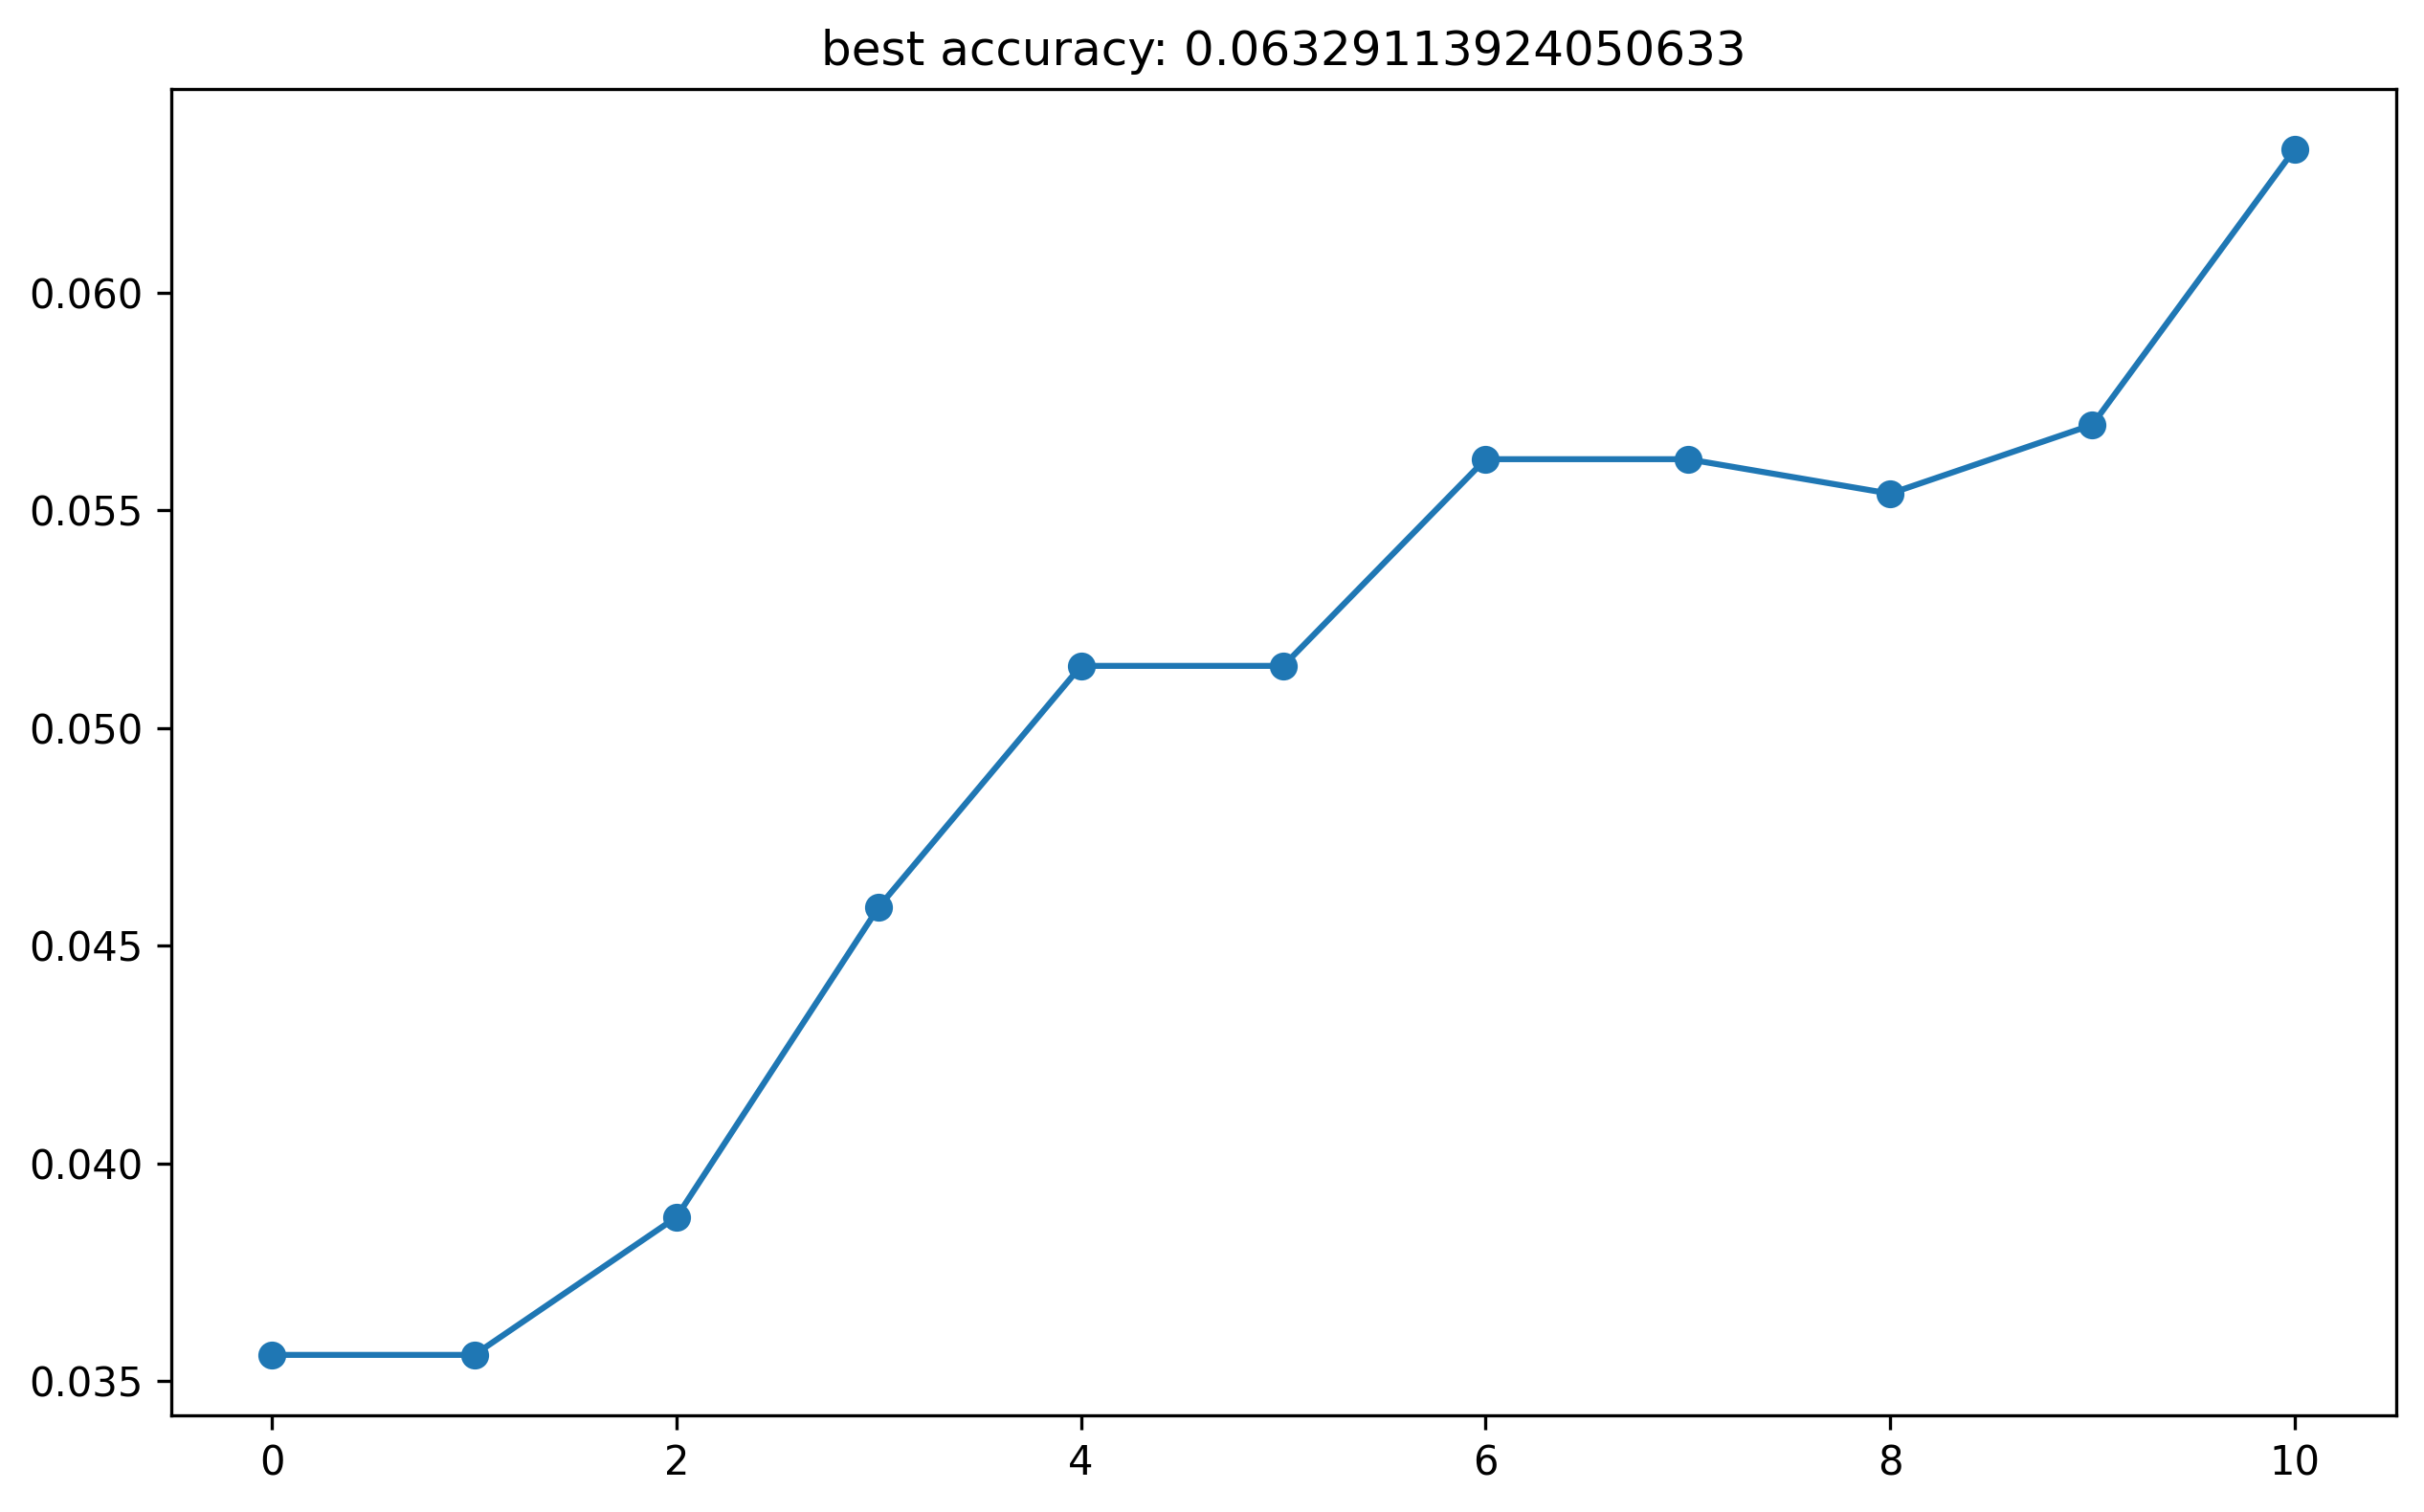
\includegraphics[width=\textwidth]{figures/unfiltered/svm_acc_1.png}
		\caption*{Accuracy (Unfiltered): 1×1m}
	\end{minipage}
\end{figure}

\begin{figure}[H]
	\centering
	\begin{minipage}{0.49\textwidth}
		\centering
		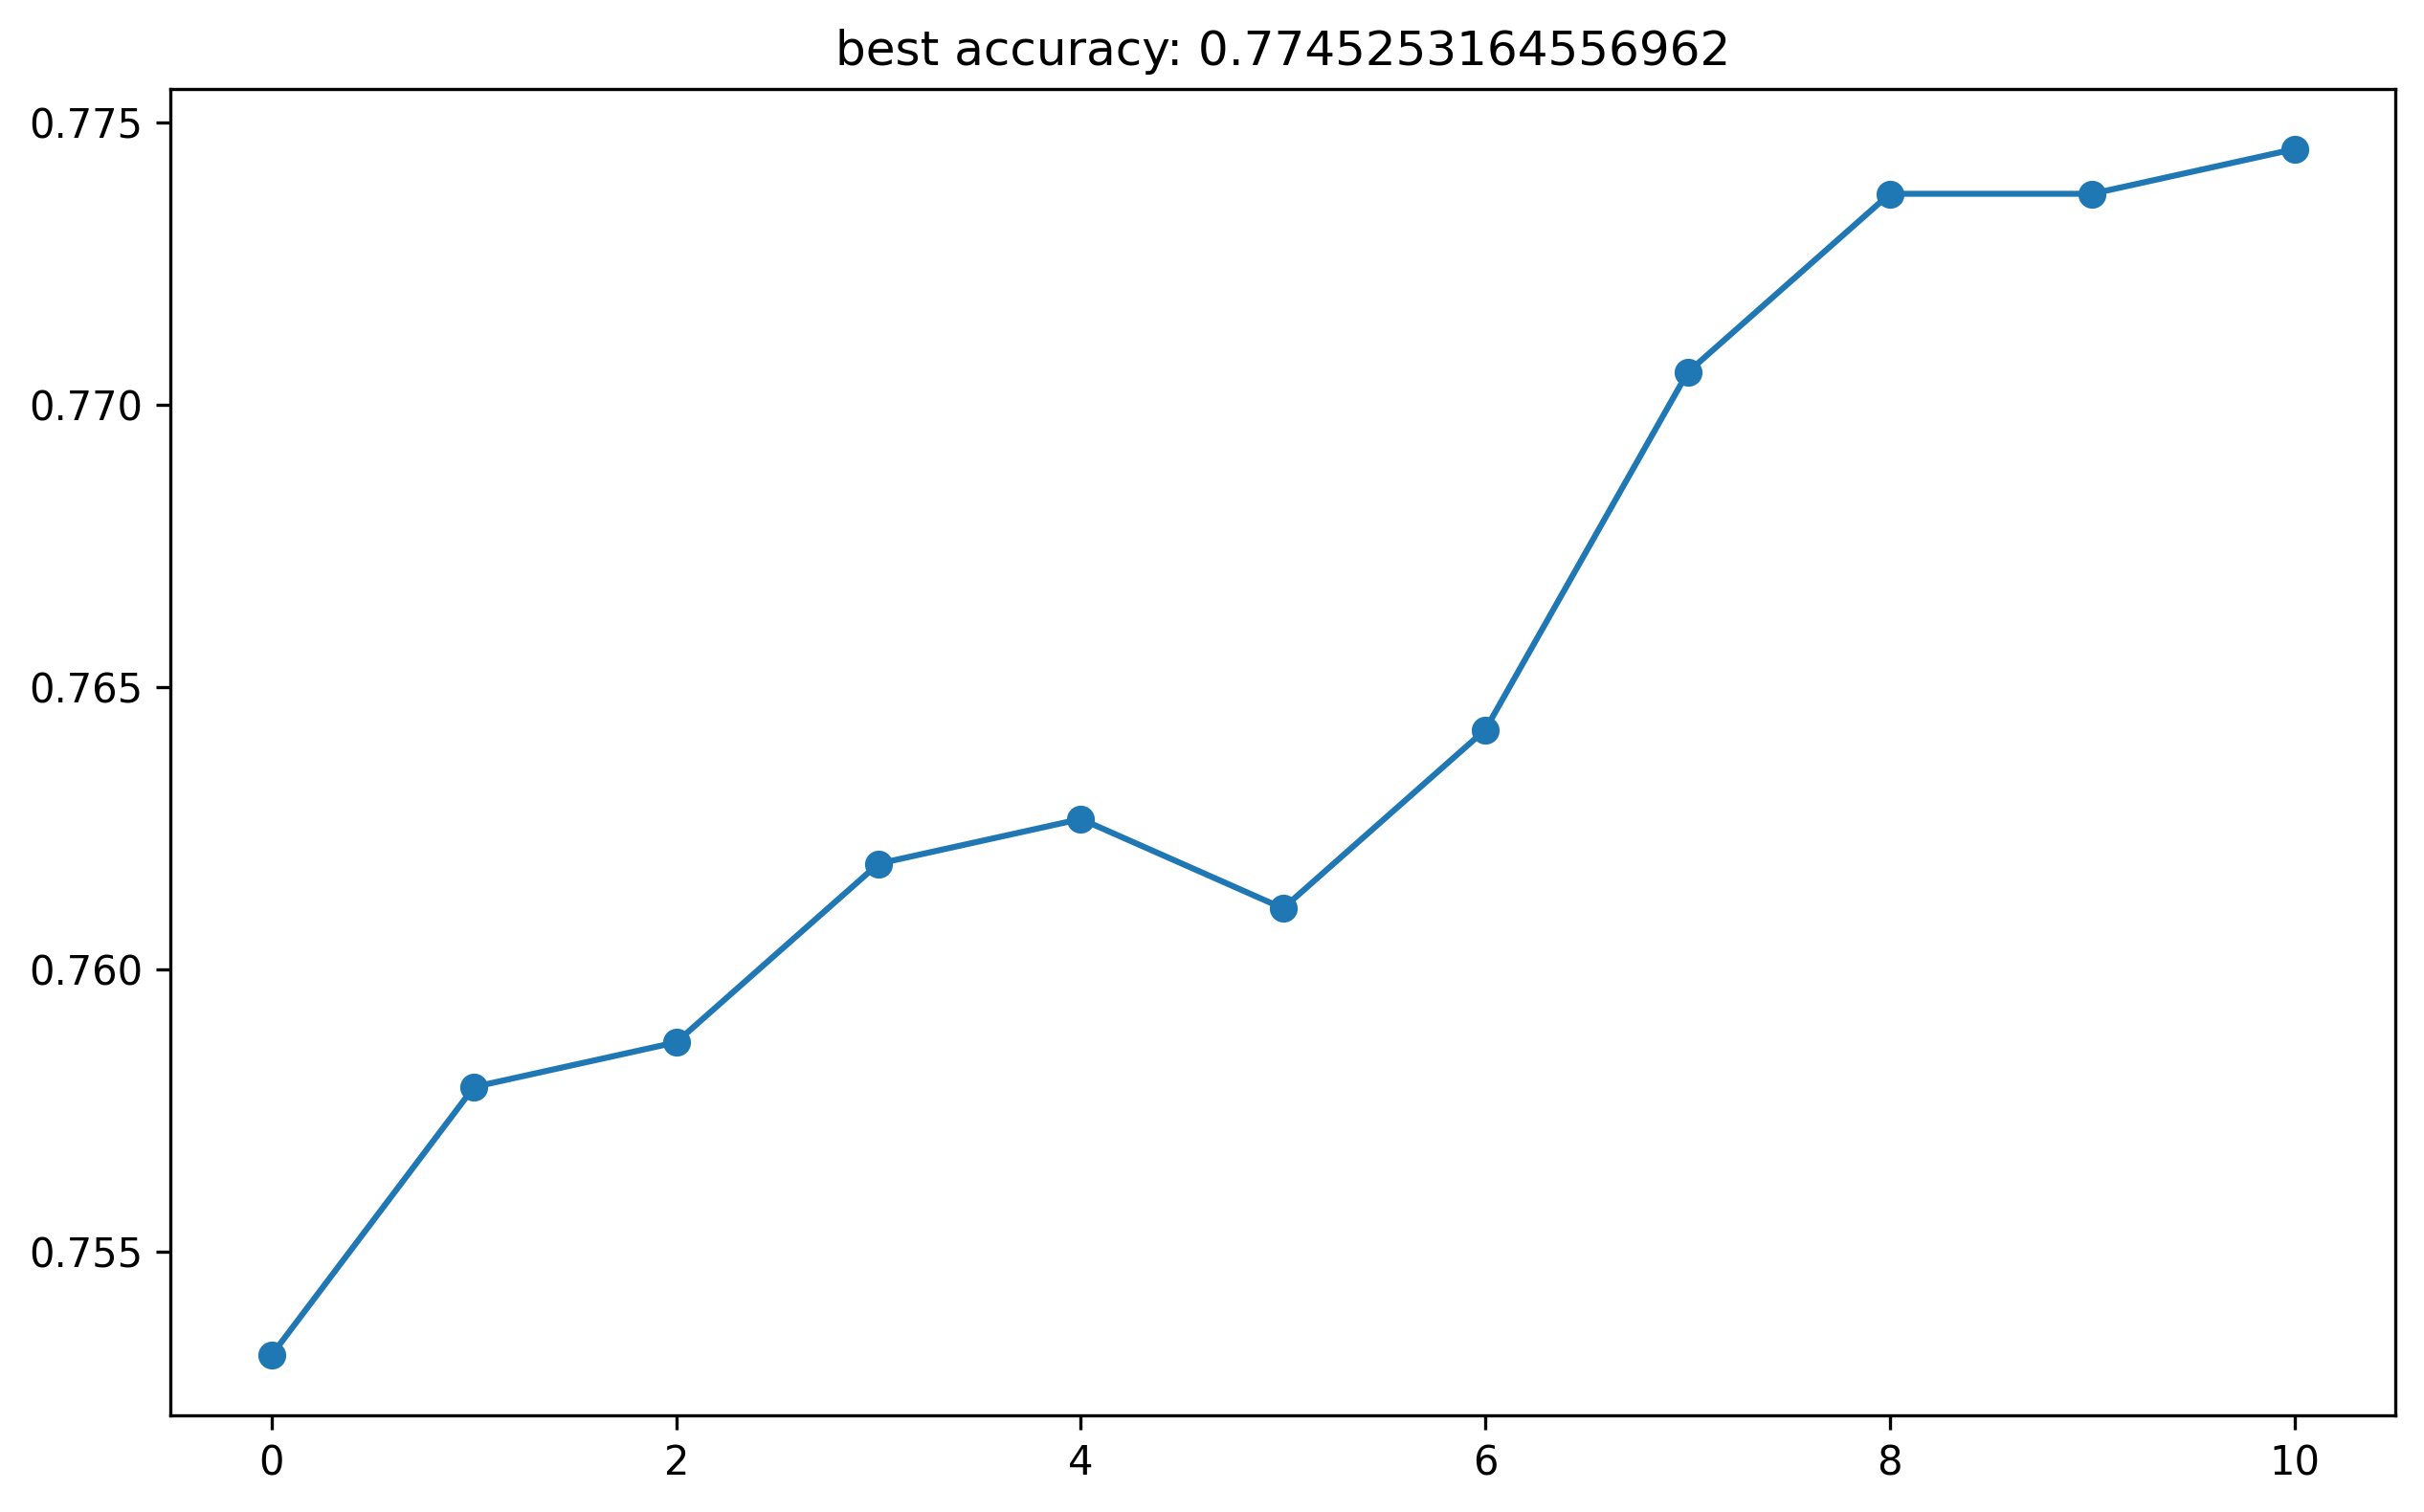
\includegraphics[width=\textwidth]{figures/filtered/svm_acc_7.png}
		\caption*{Accuracy (Filtered): 7×7m}
	\end{minipage}
	\hfill
	\begin{minipage}{0.49\textwidth}
		\centering
		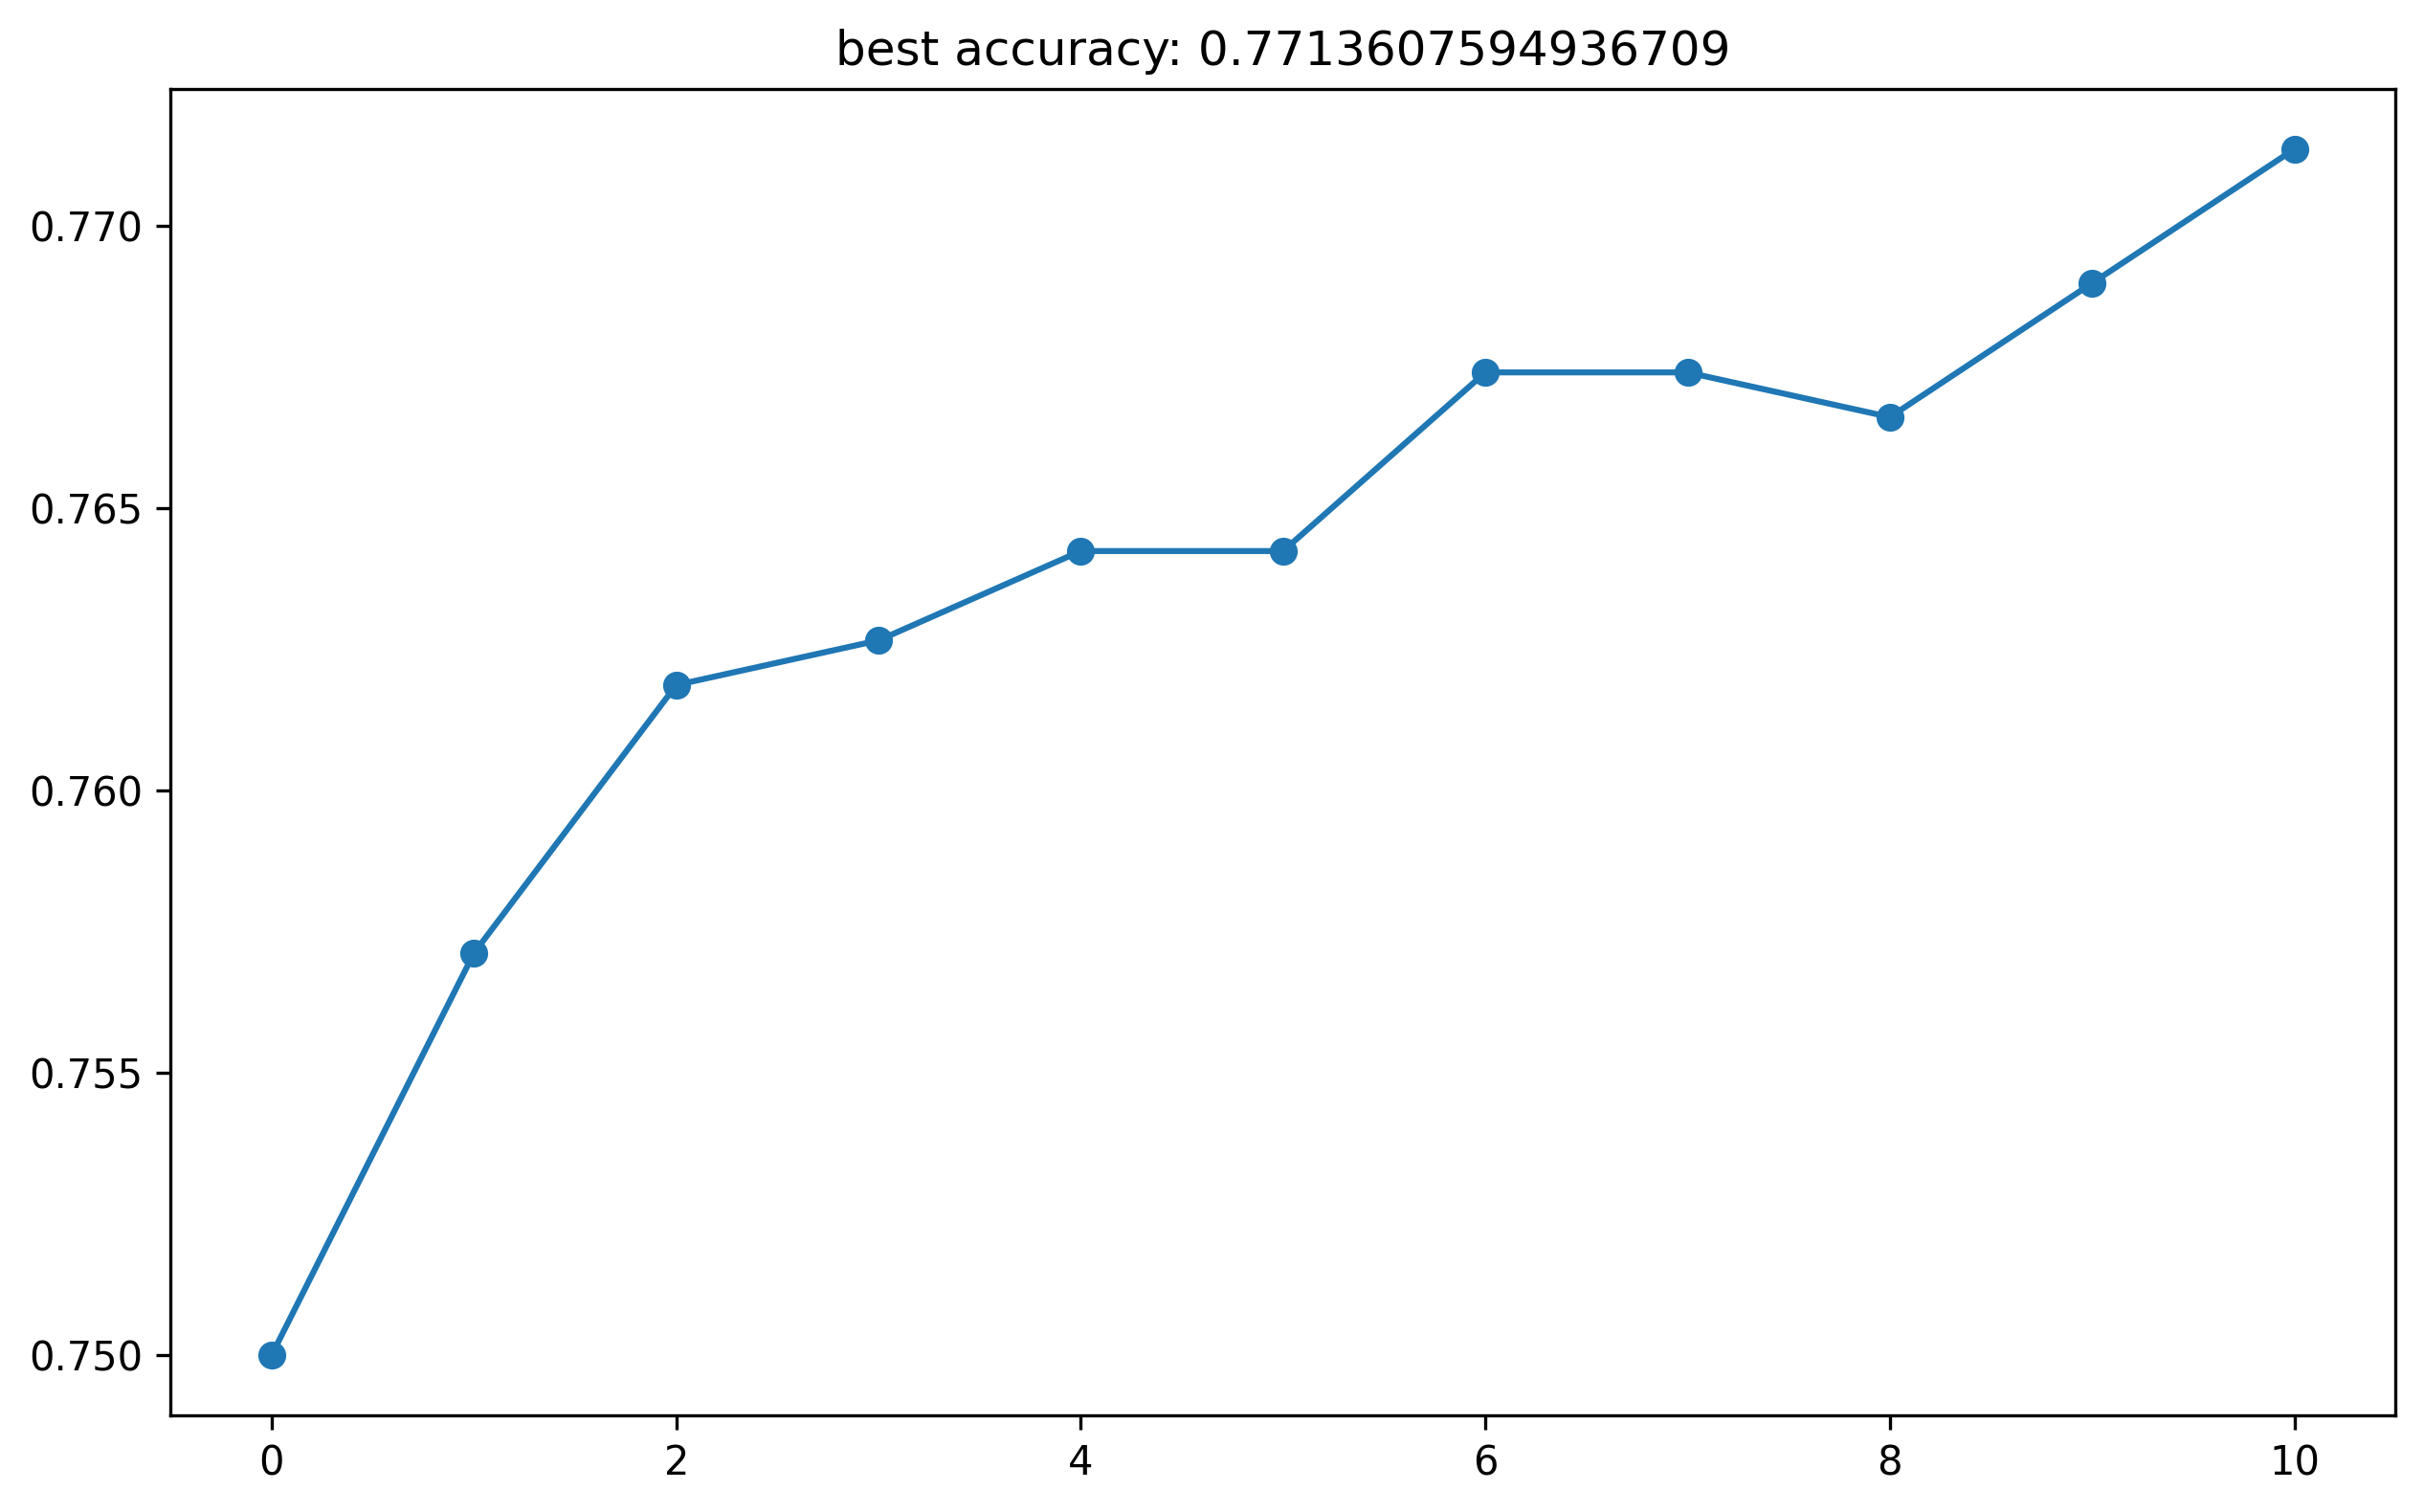
\includegraphics[width=\textwidth]{figures/unfiltered/svm_acc_7.png}
		\caption*{Accuracy (Unfiltered): 7×7m}
	\end{minipage}
\end{figure}

\begin{figure}[H]
	\centering
	\begin{minipage}{0.49\textwidth}
		\centering
		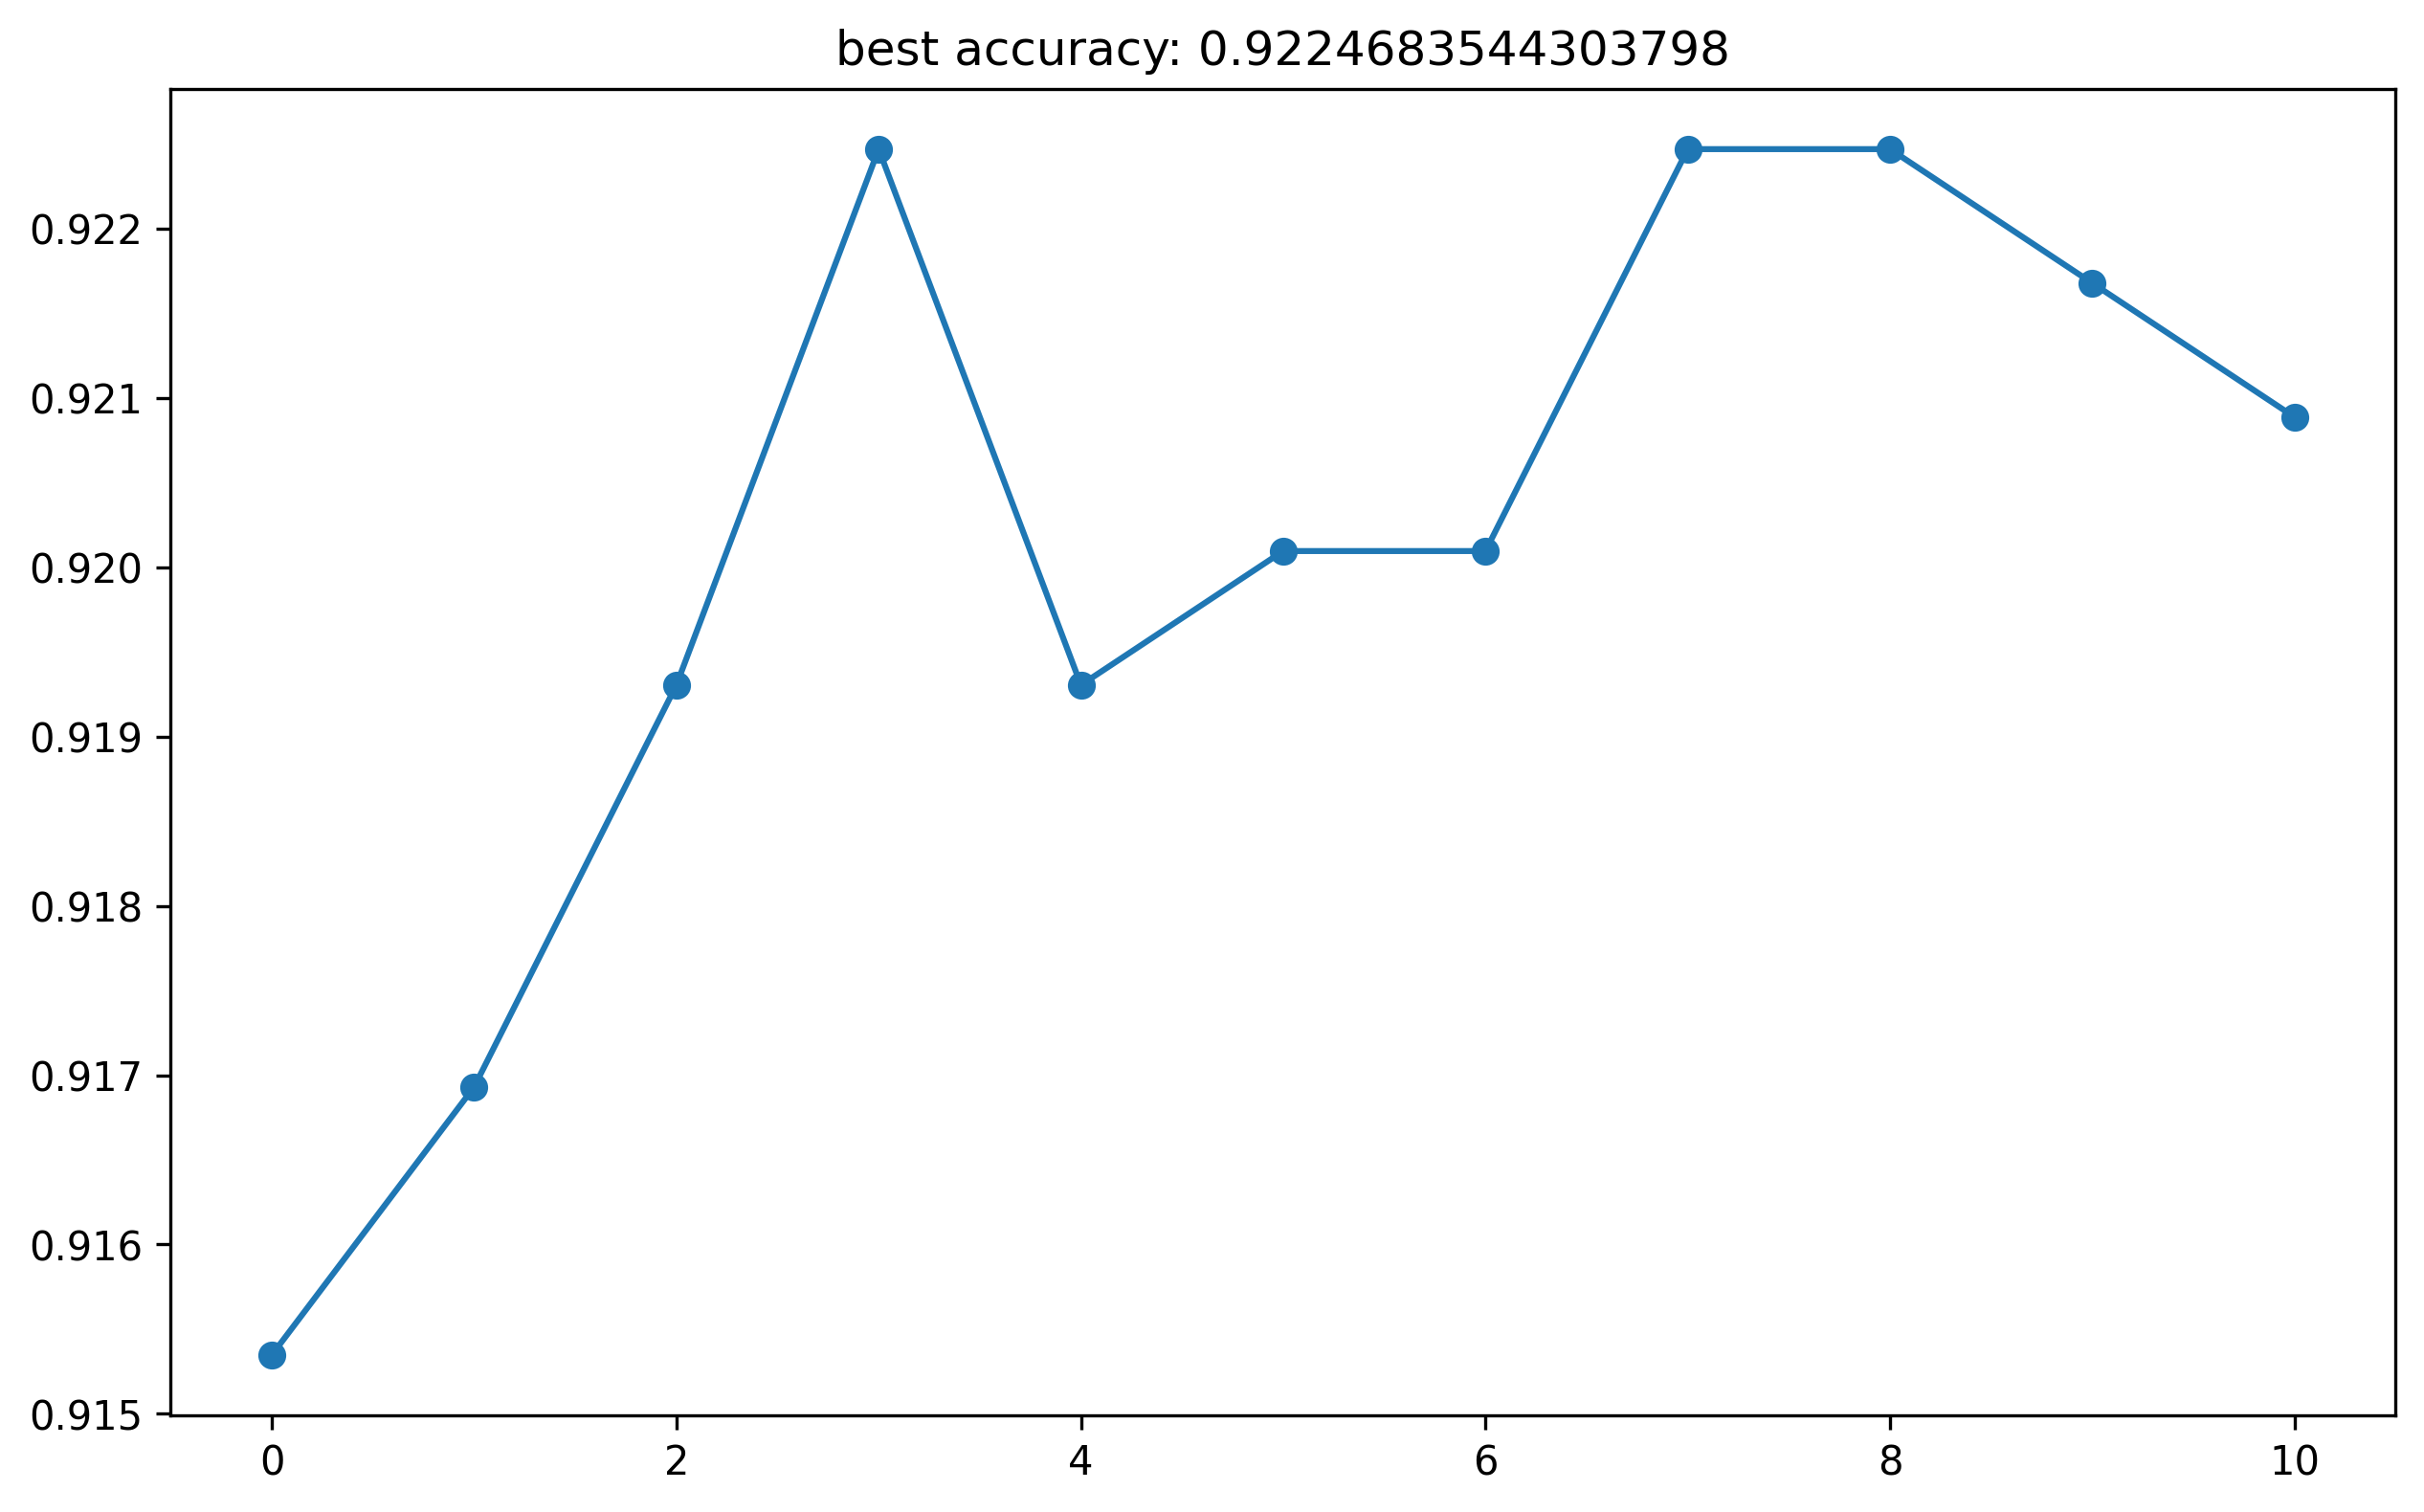
\includegraphics[width=\textwidth]{figures/filtered/svm_acc_15.png}
		\caption*{Accuracy (Filtered): 15×15m}
	\end{minipage}
	\hfill
	\begin{minipage}{0.49\textwidth}
		\centering
		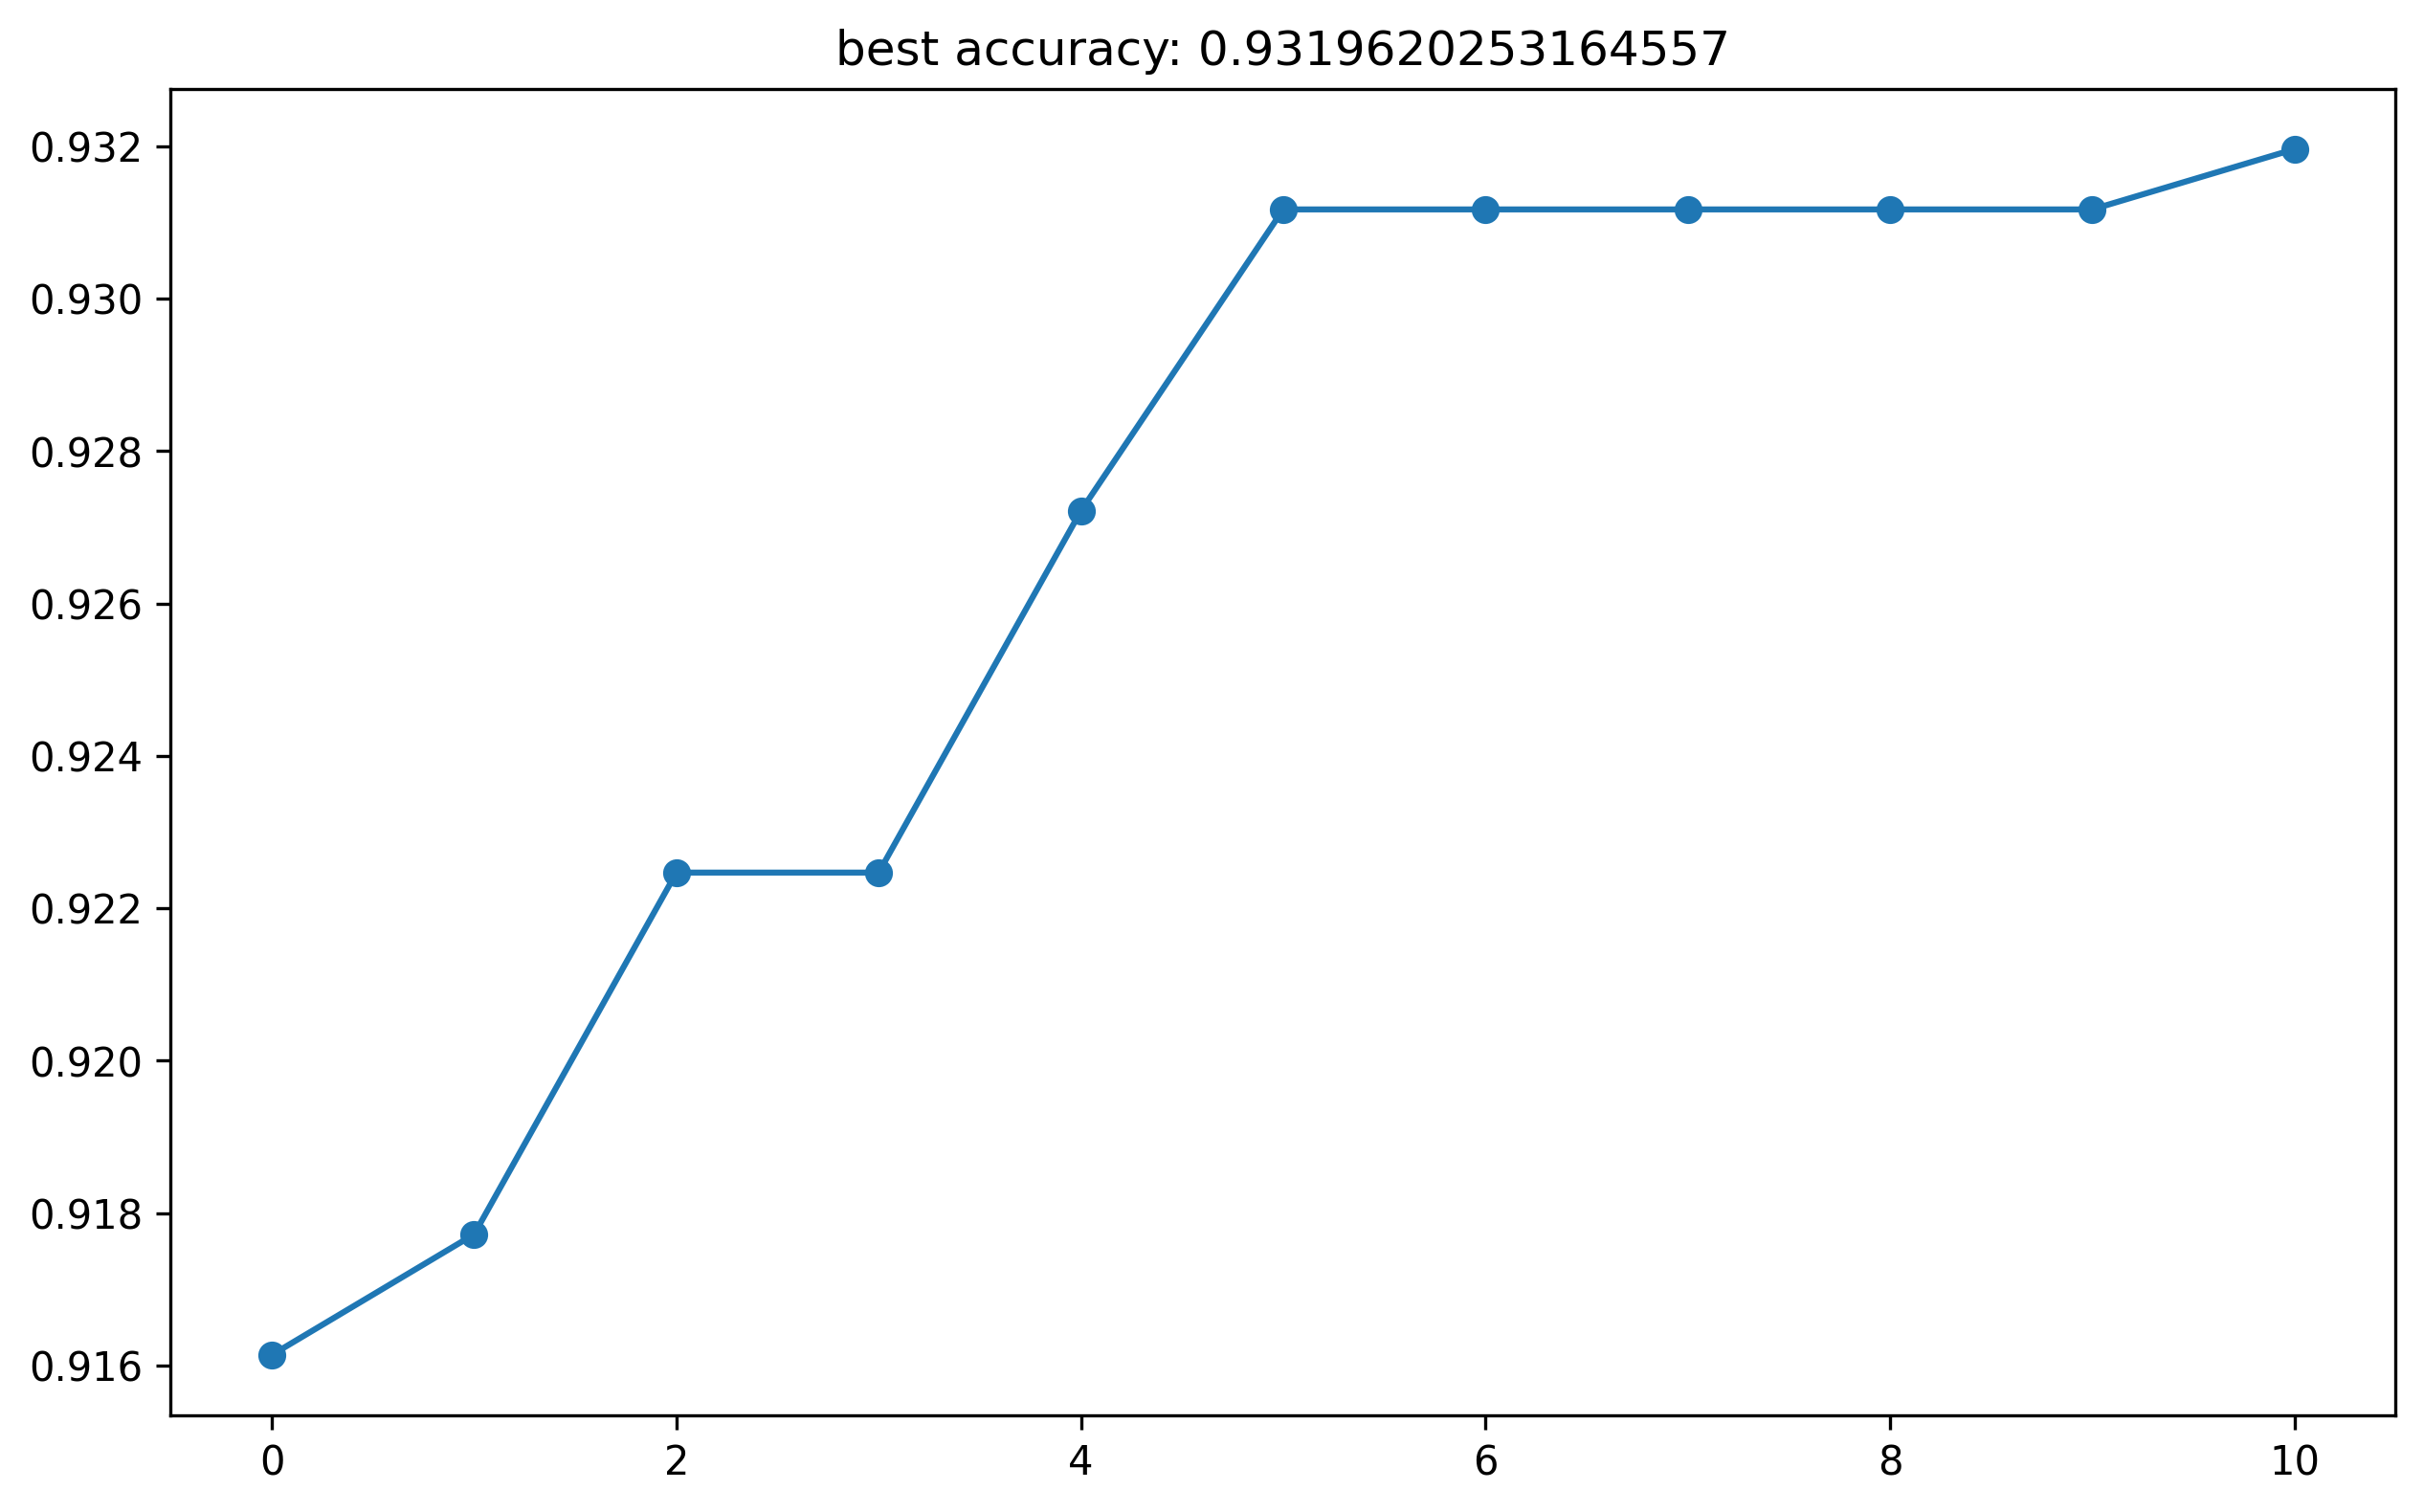
\includegraphics[width=\textwidth]{figures/unfiltered/svm_acc_15.png}
		\caption*{Accuracy (Unfiltered): 15×15m}
	\end{minipage}
\end{figure}

\begin{figure}[H]
	\centering
	\begin{minipage}{0.49\textwidth}
		\centering
		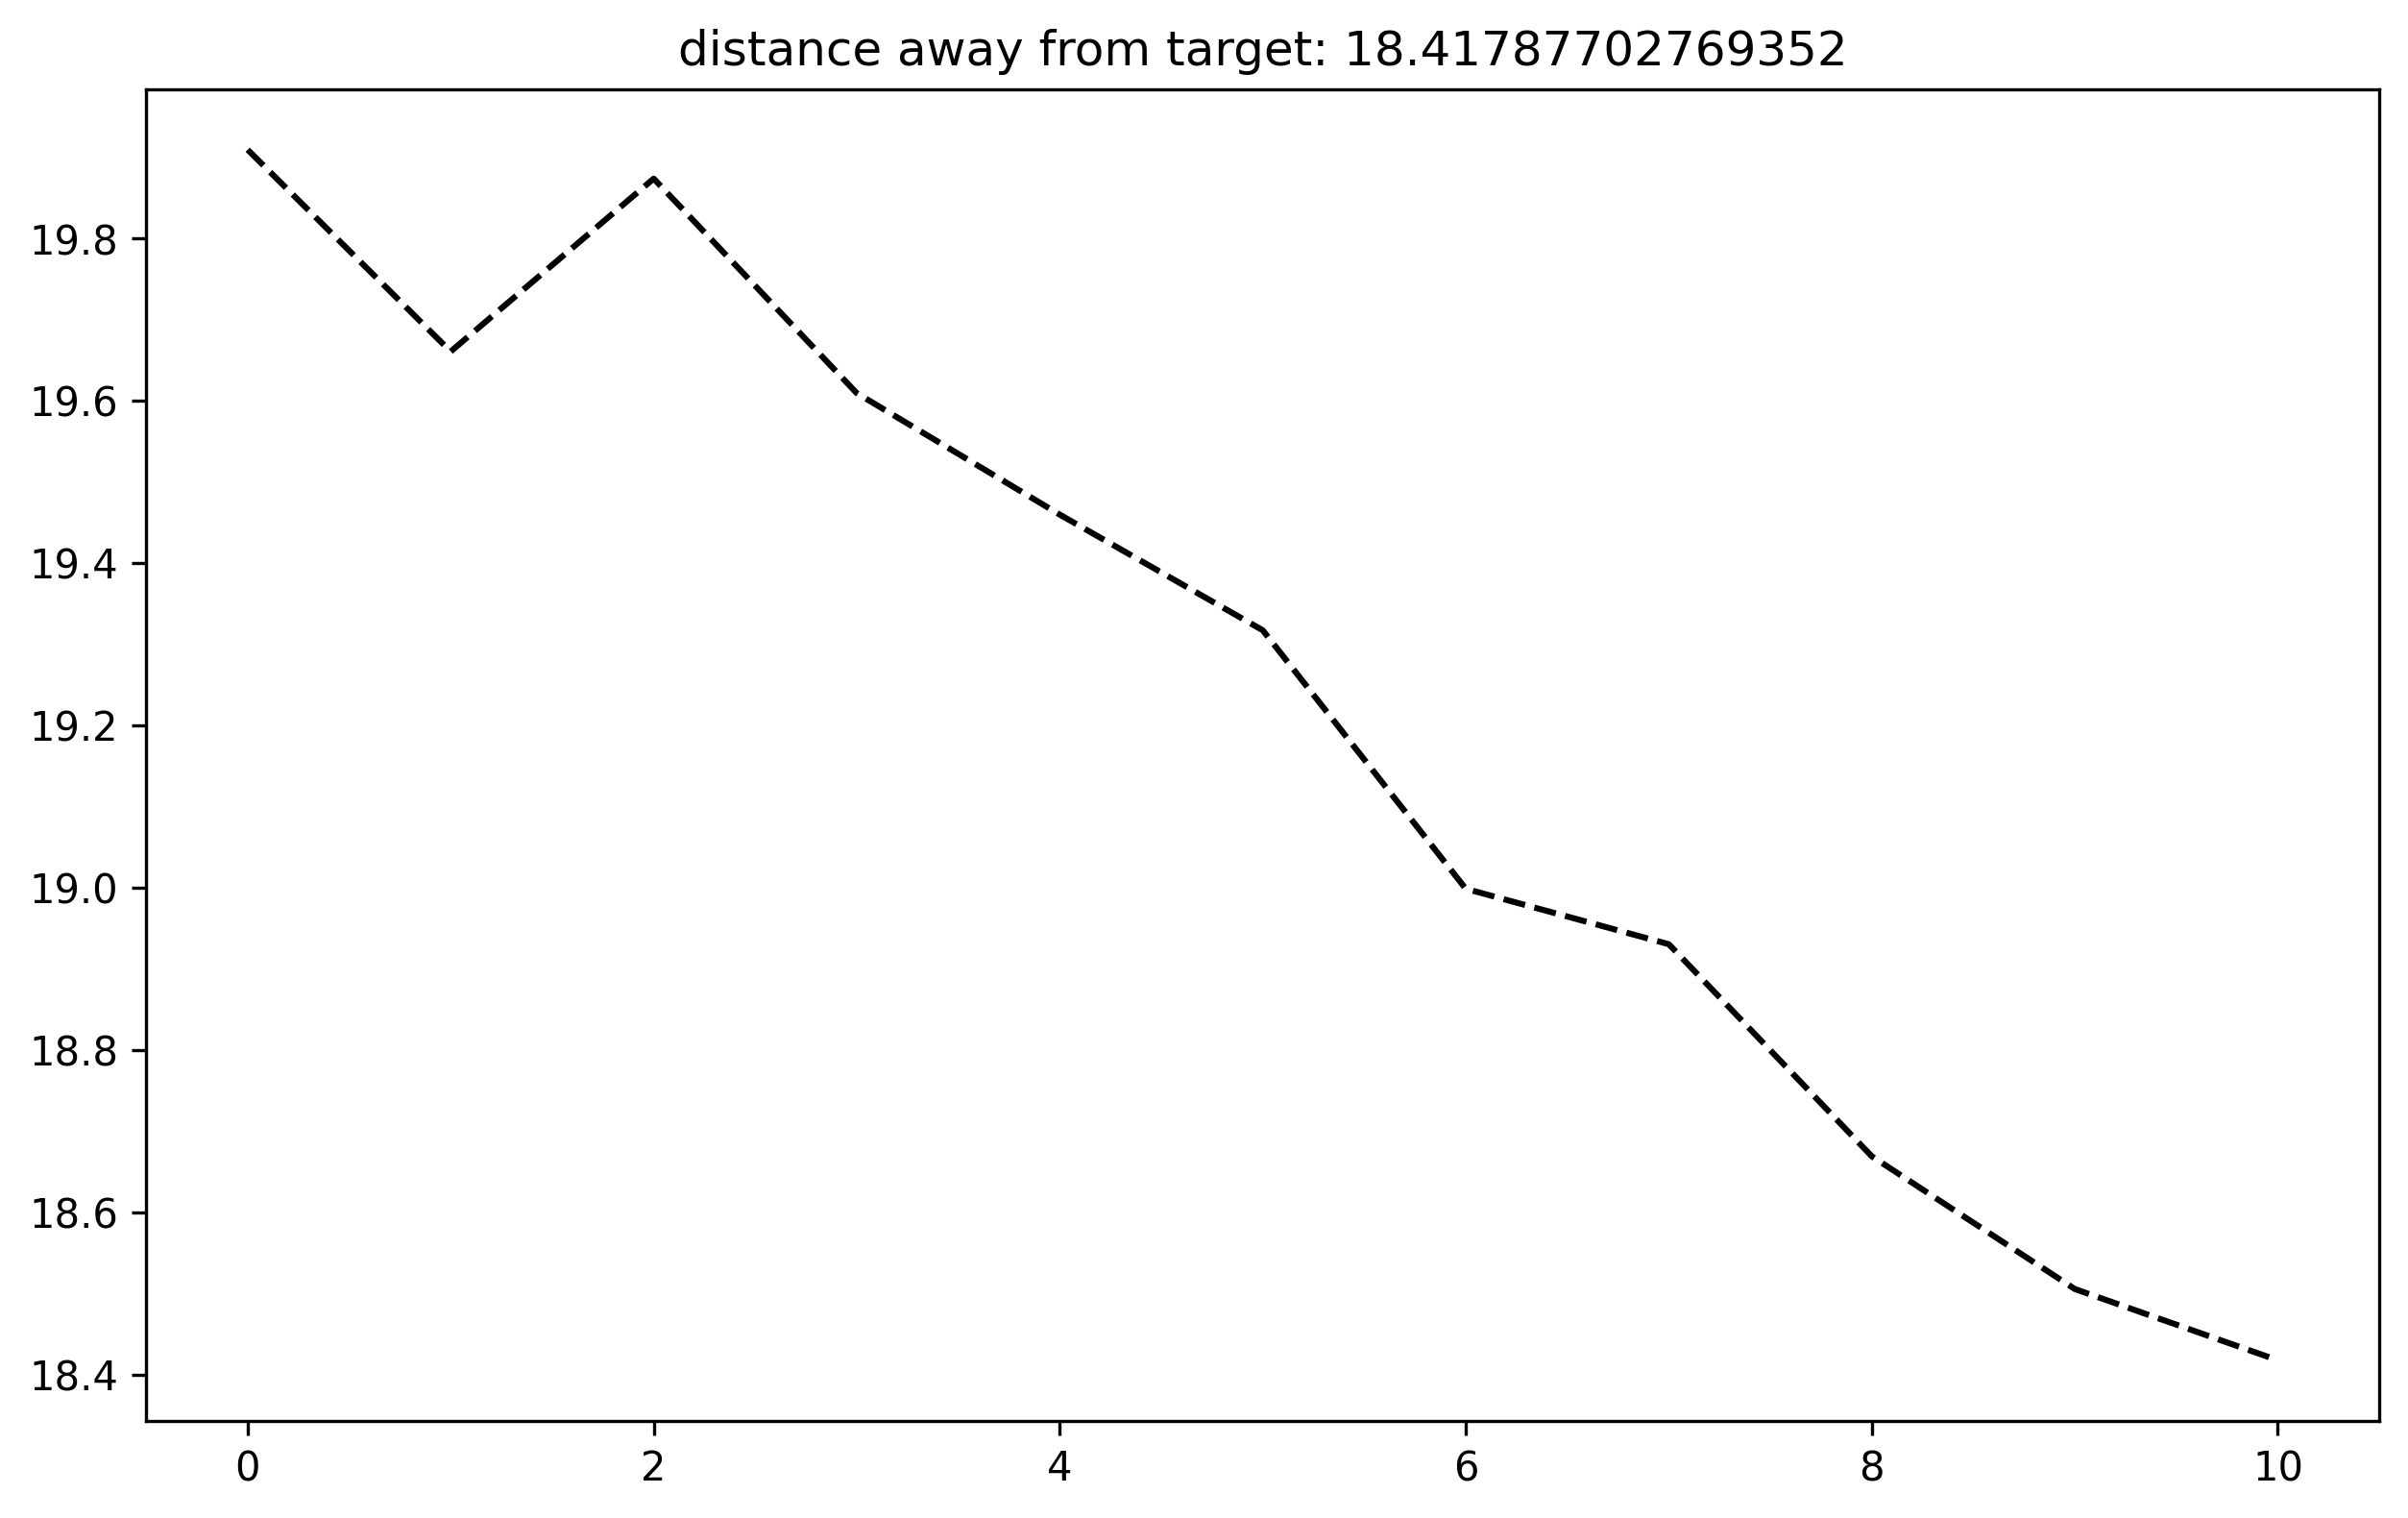
\includegraphics[width=\textwidth]{figures/filtered/svm_custom_1.png}
		\caption*{AGT (Filtered): 1×1m}
	\end{minipage}
	\hfill
	\begin{minipage}{0.49\textwidth}
		\centering
		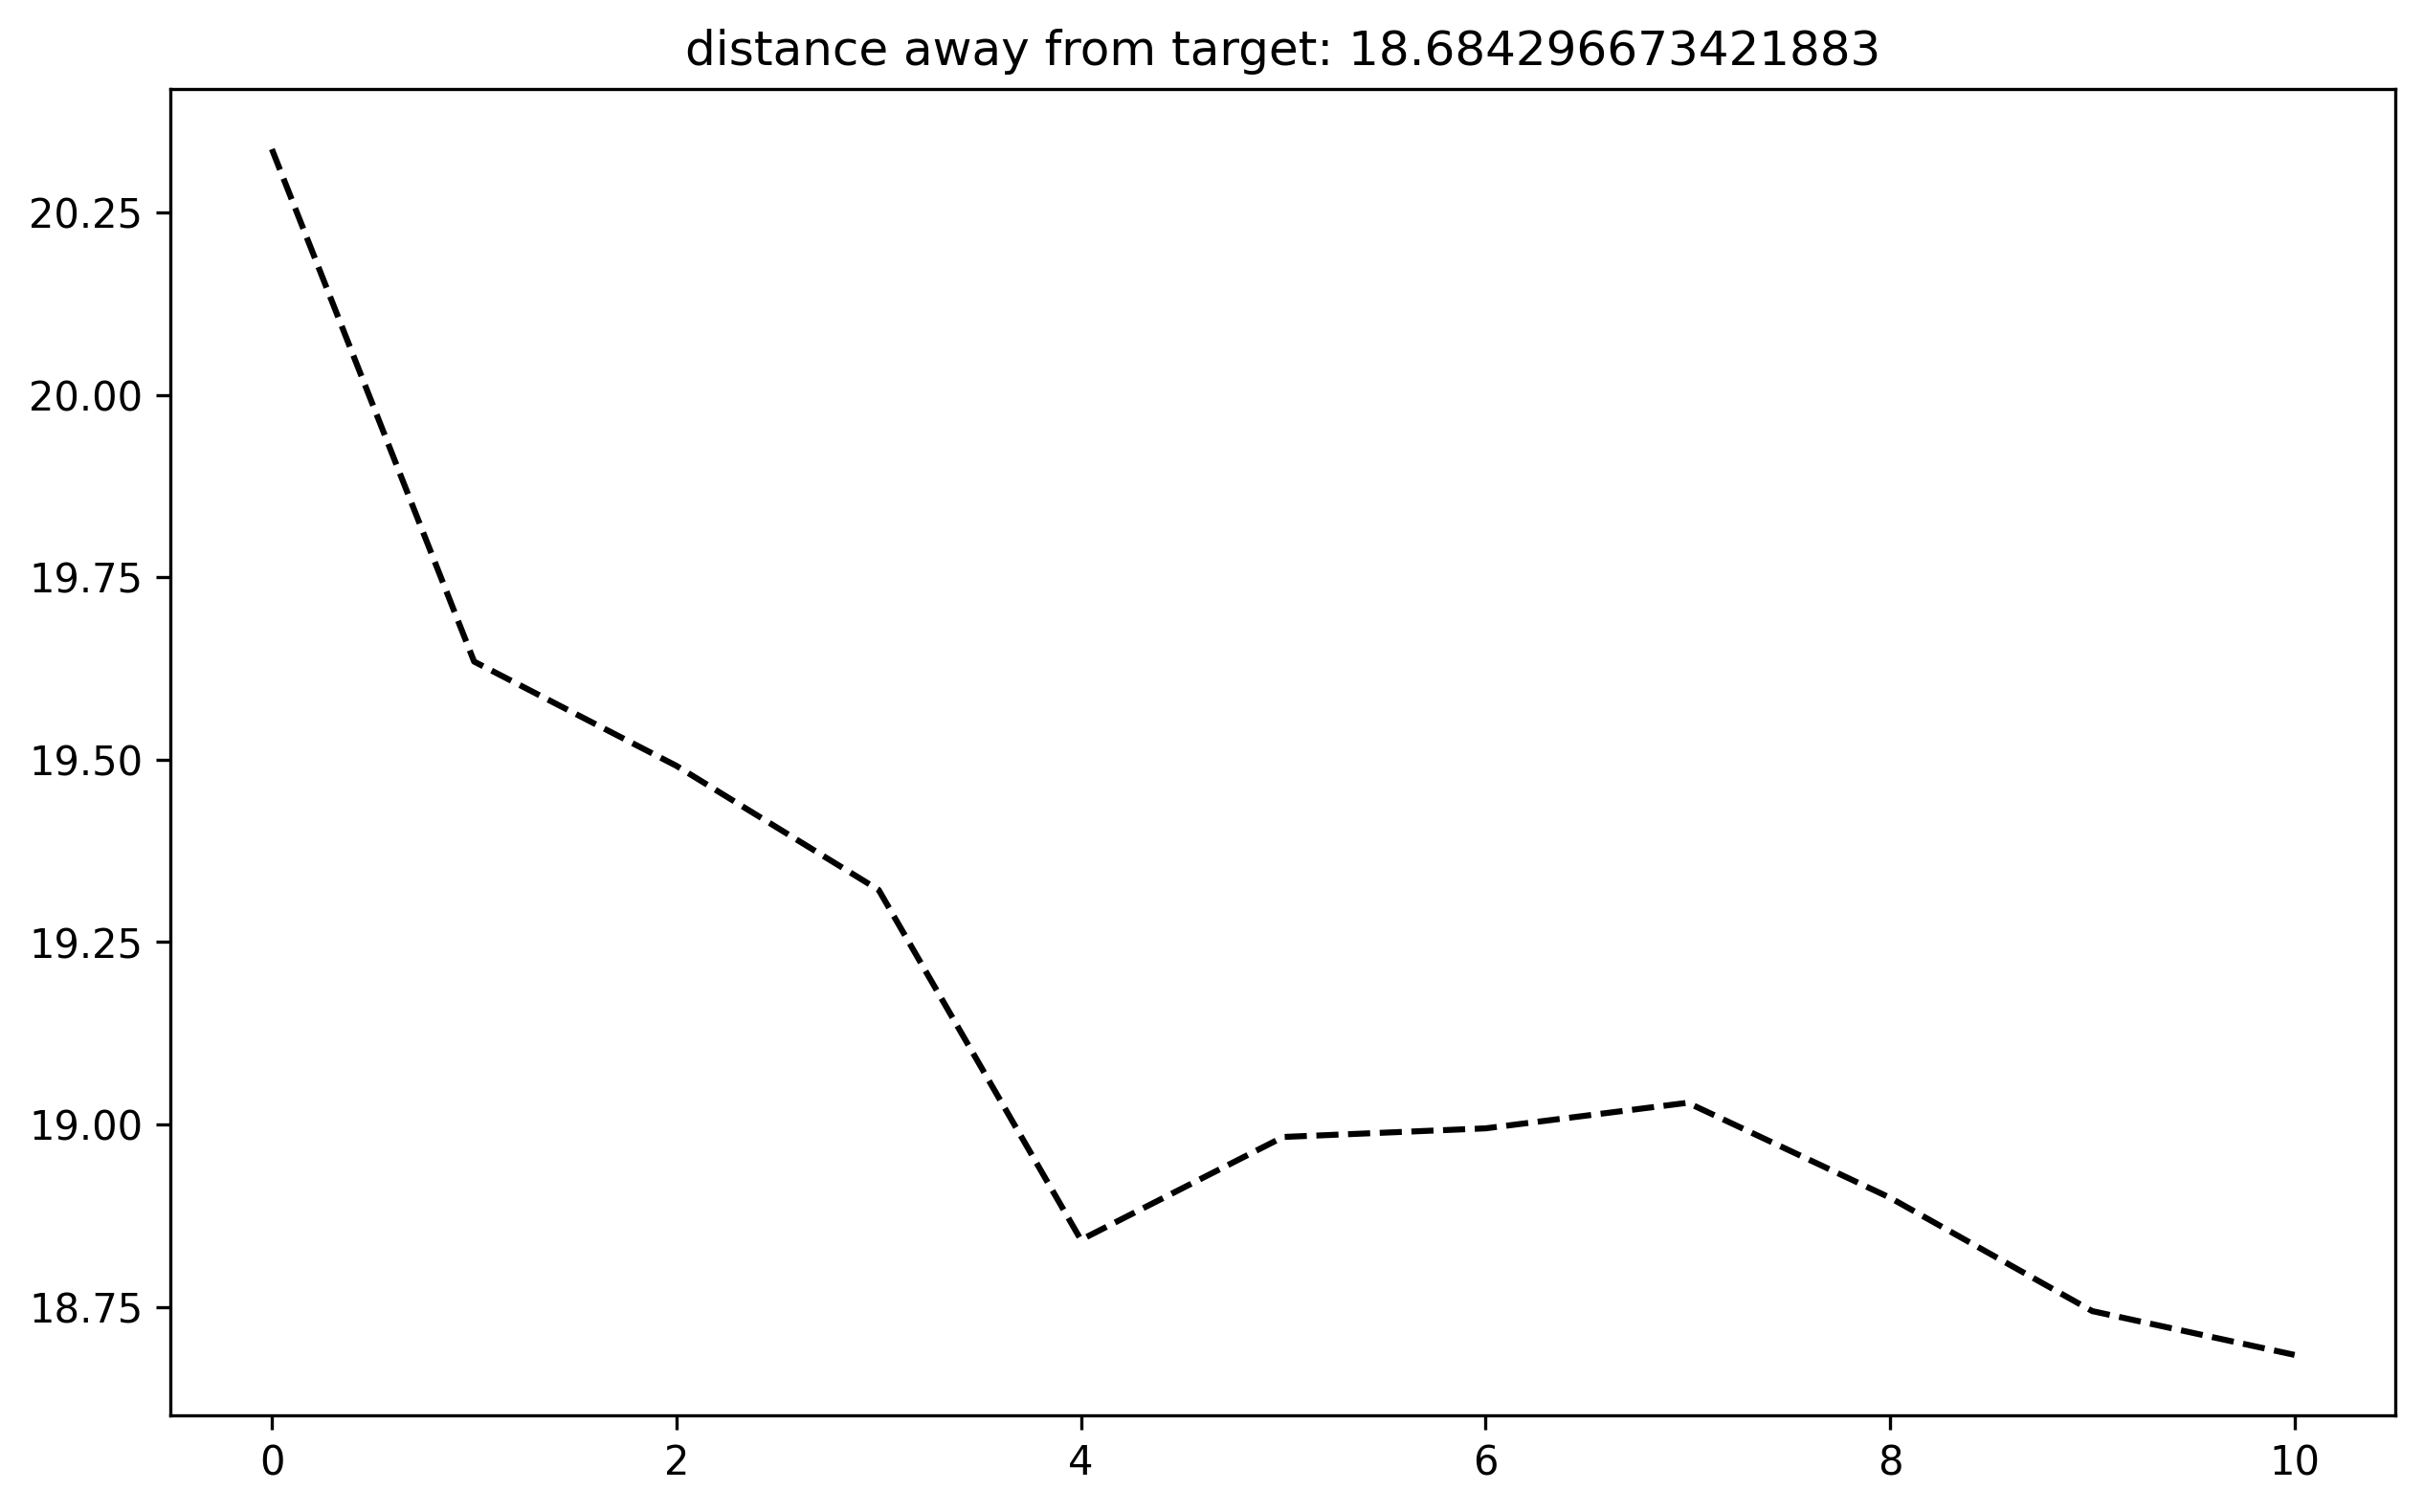
\includegraphics[width=\textwidth]{figures/unfiltered/svm_custom_1.png}
		\caption*{AGT (Unfiltered): 1×1m}
	\end{minipage}
\end{figure}

\begin{figure}[H]
	\centering
	\begin{minipage}{0.49\textwidth}
		\centering
		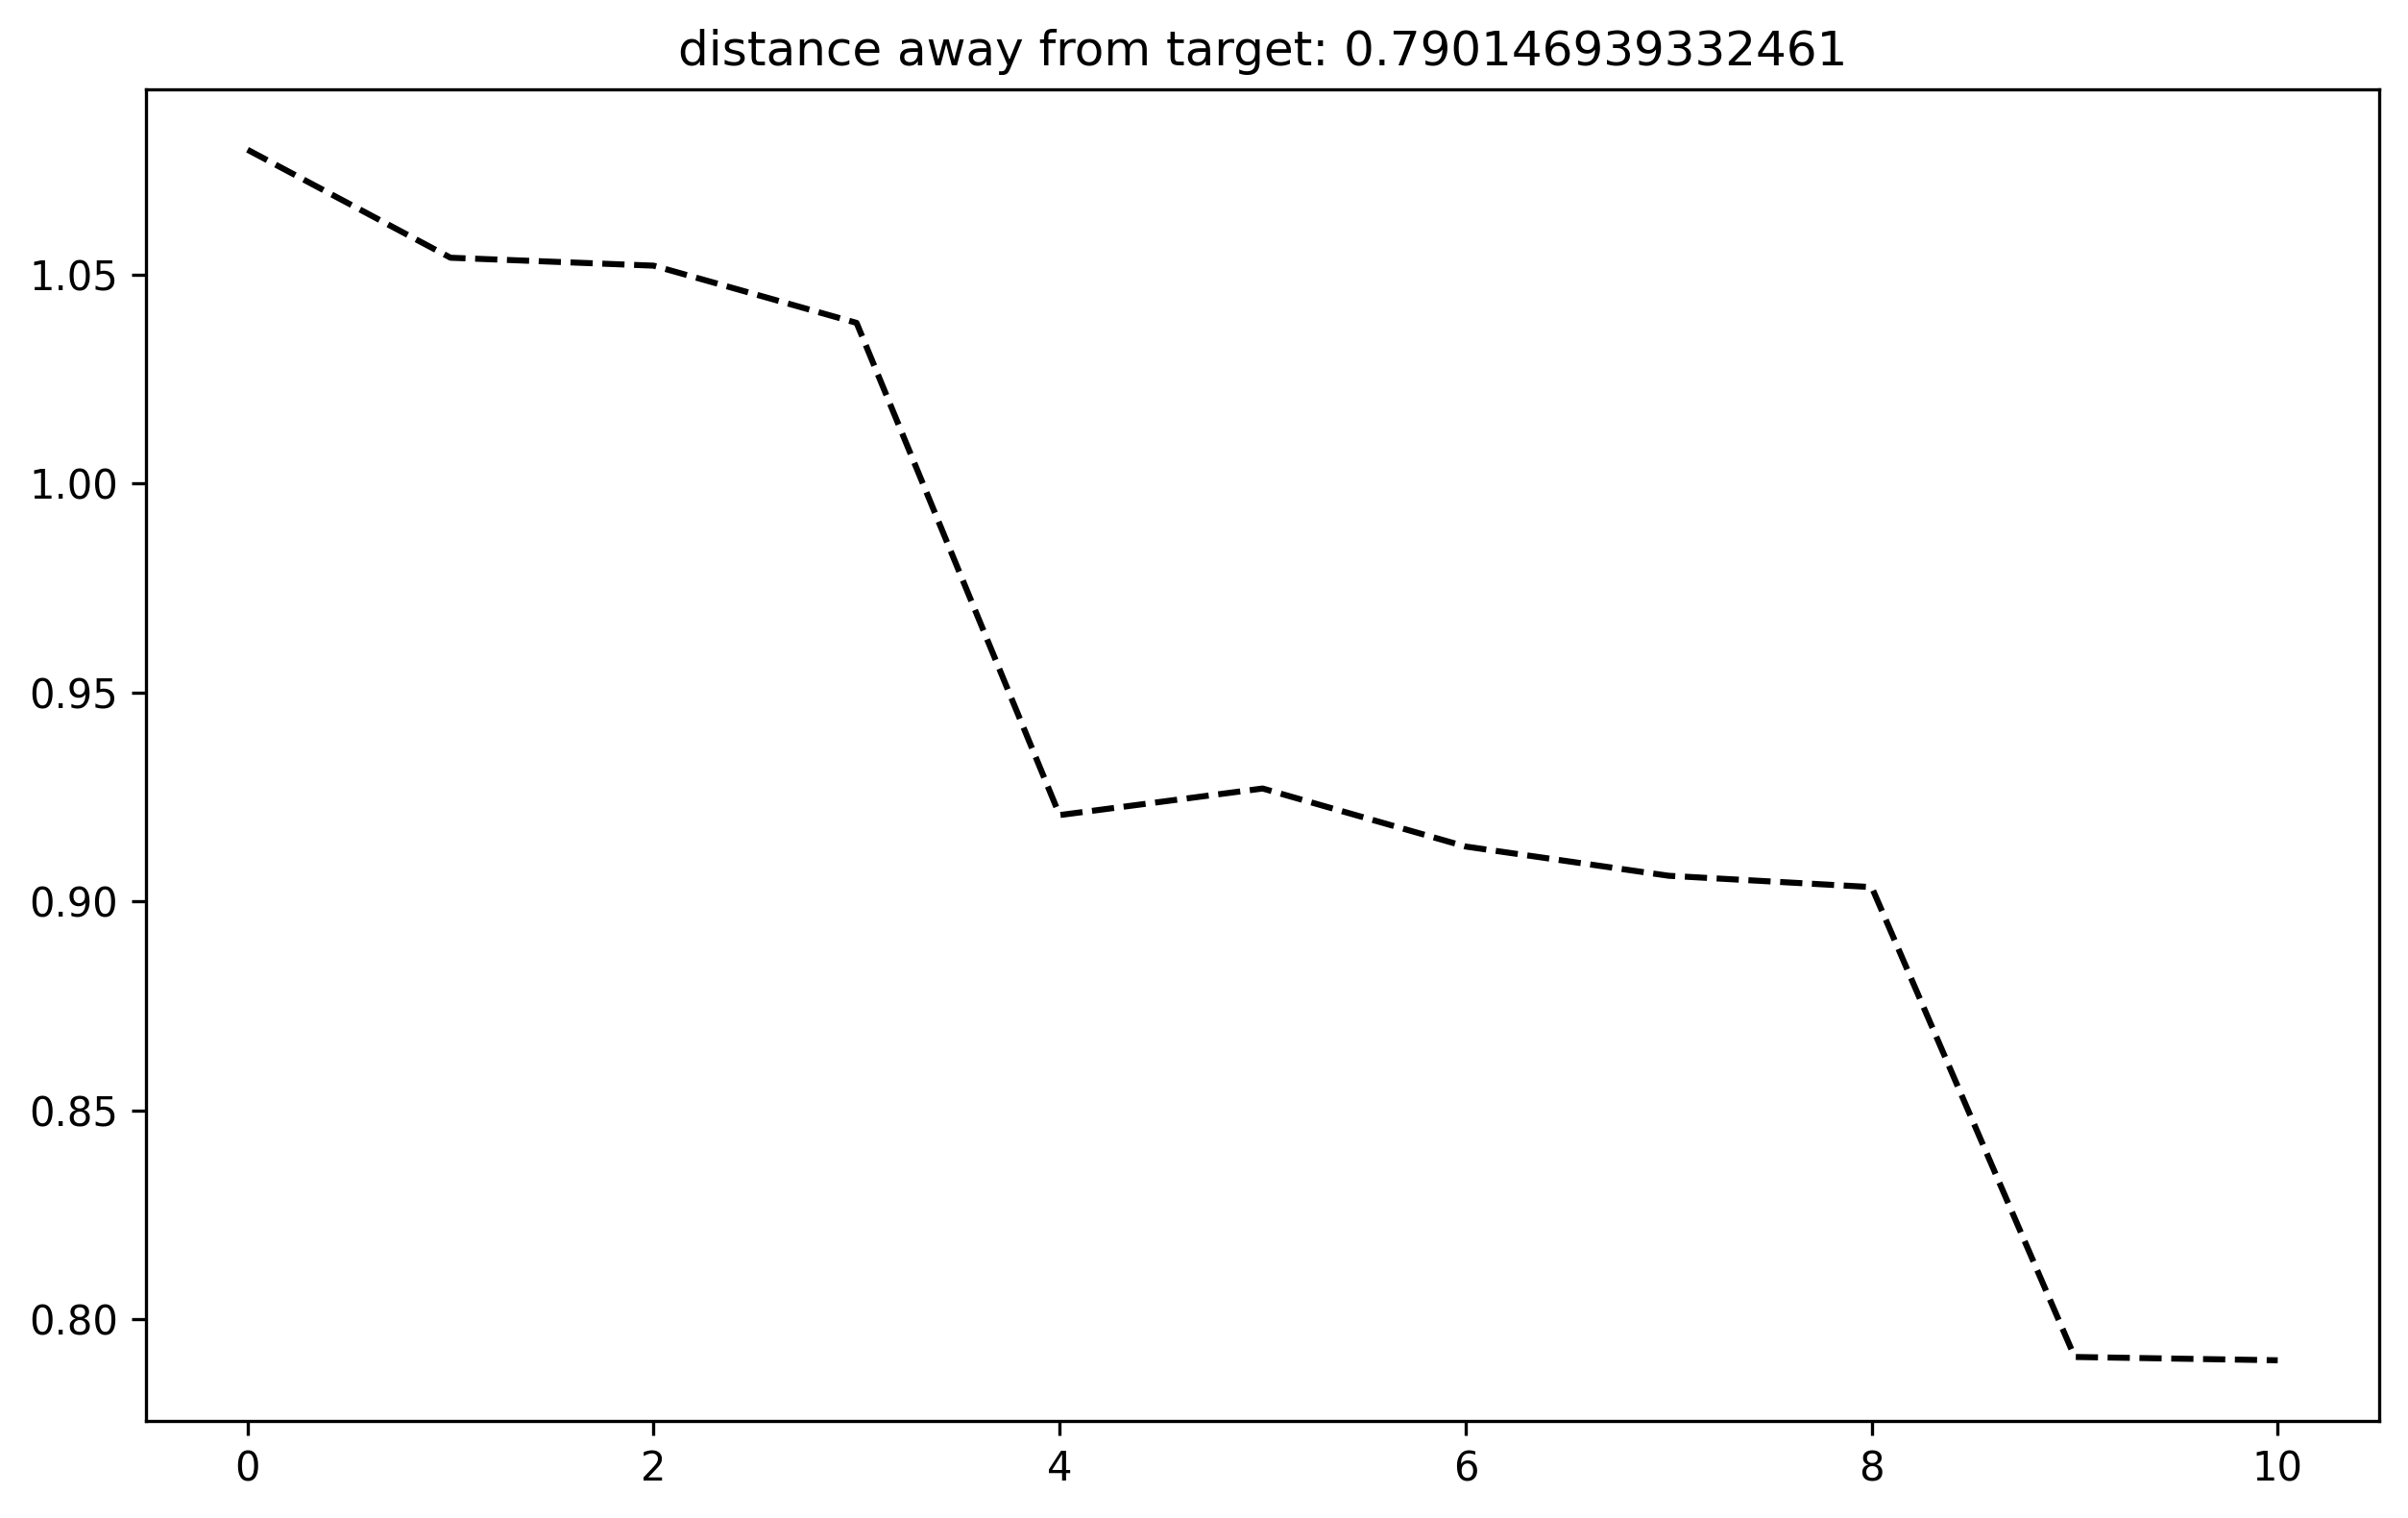
\includegraphics[width=\textwidth]{figures/filtered/svm_custom_7.png}
		\caption*{AGT (Filtered): 7×7m}
	\end{minipage}
	\hfill
	\begin{minipage}{0.49\textwidth}
		\centering
		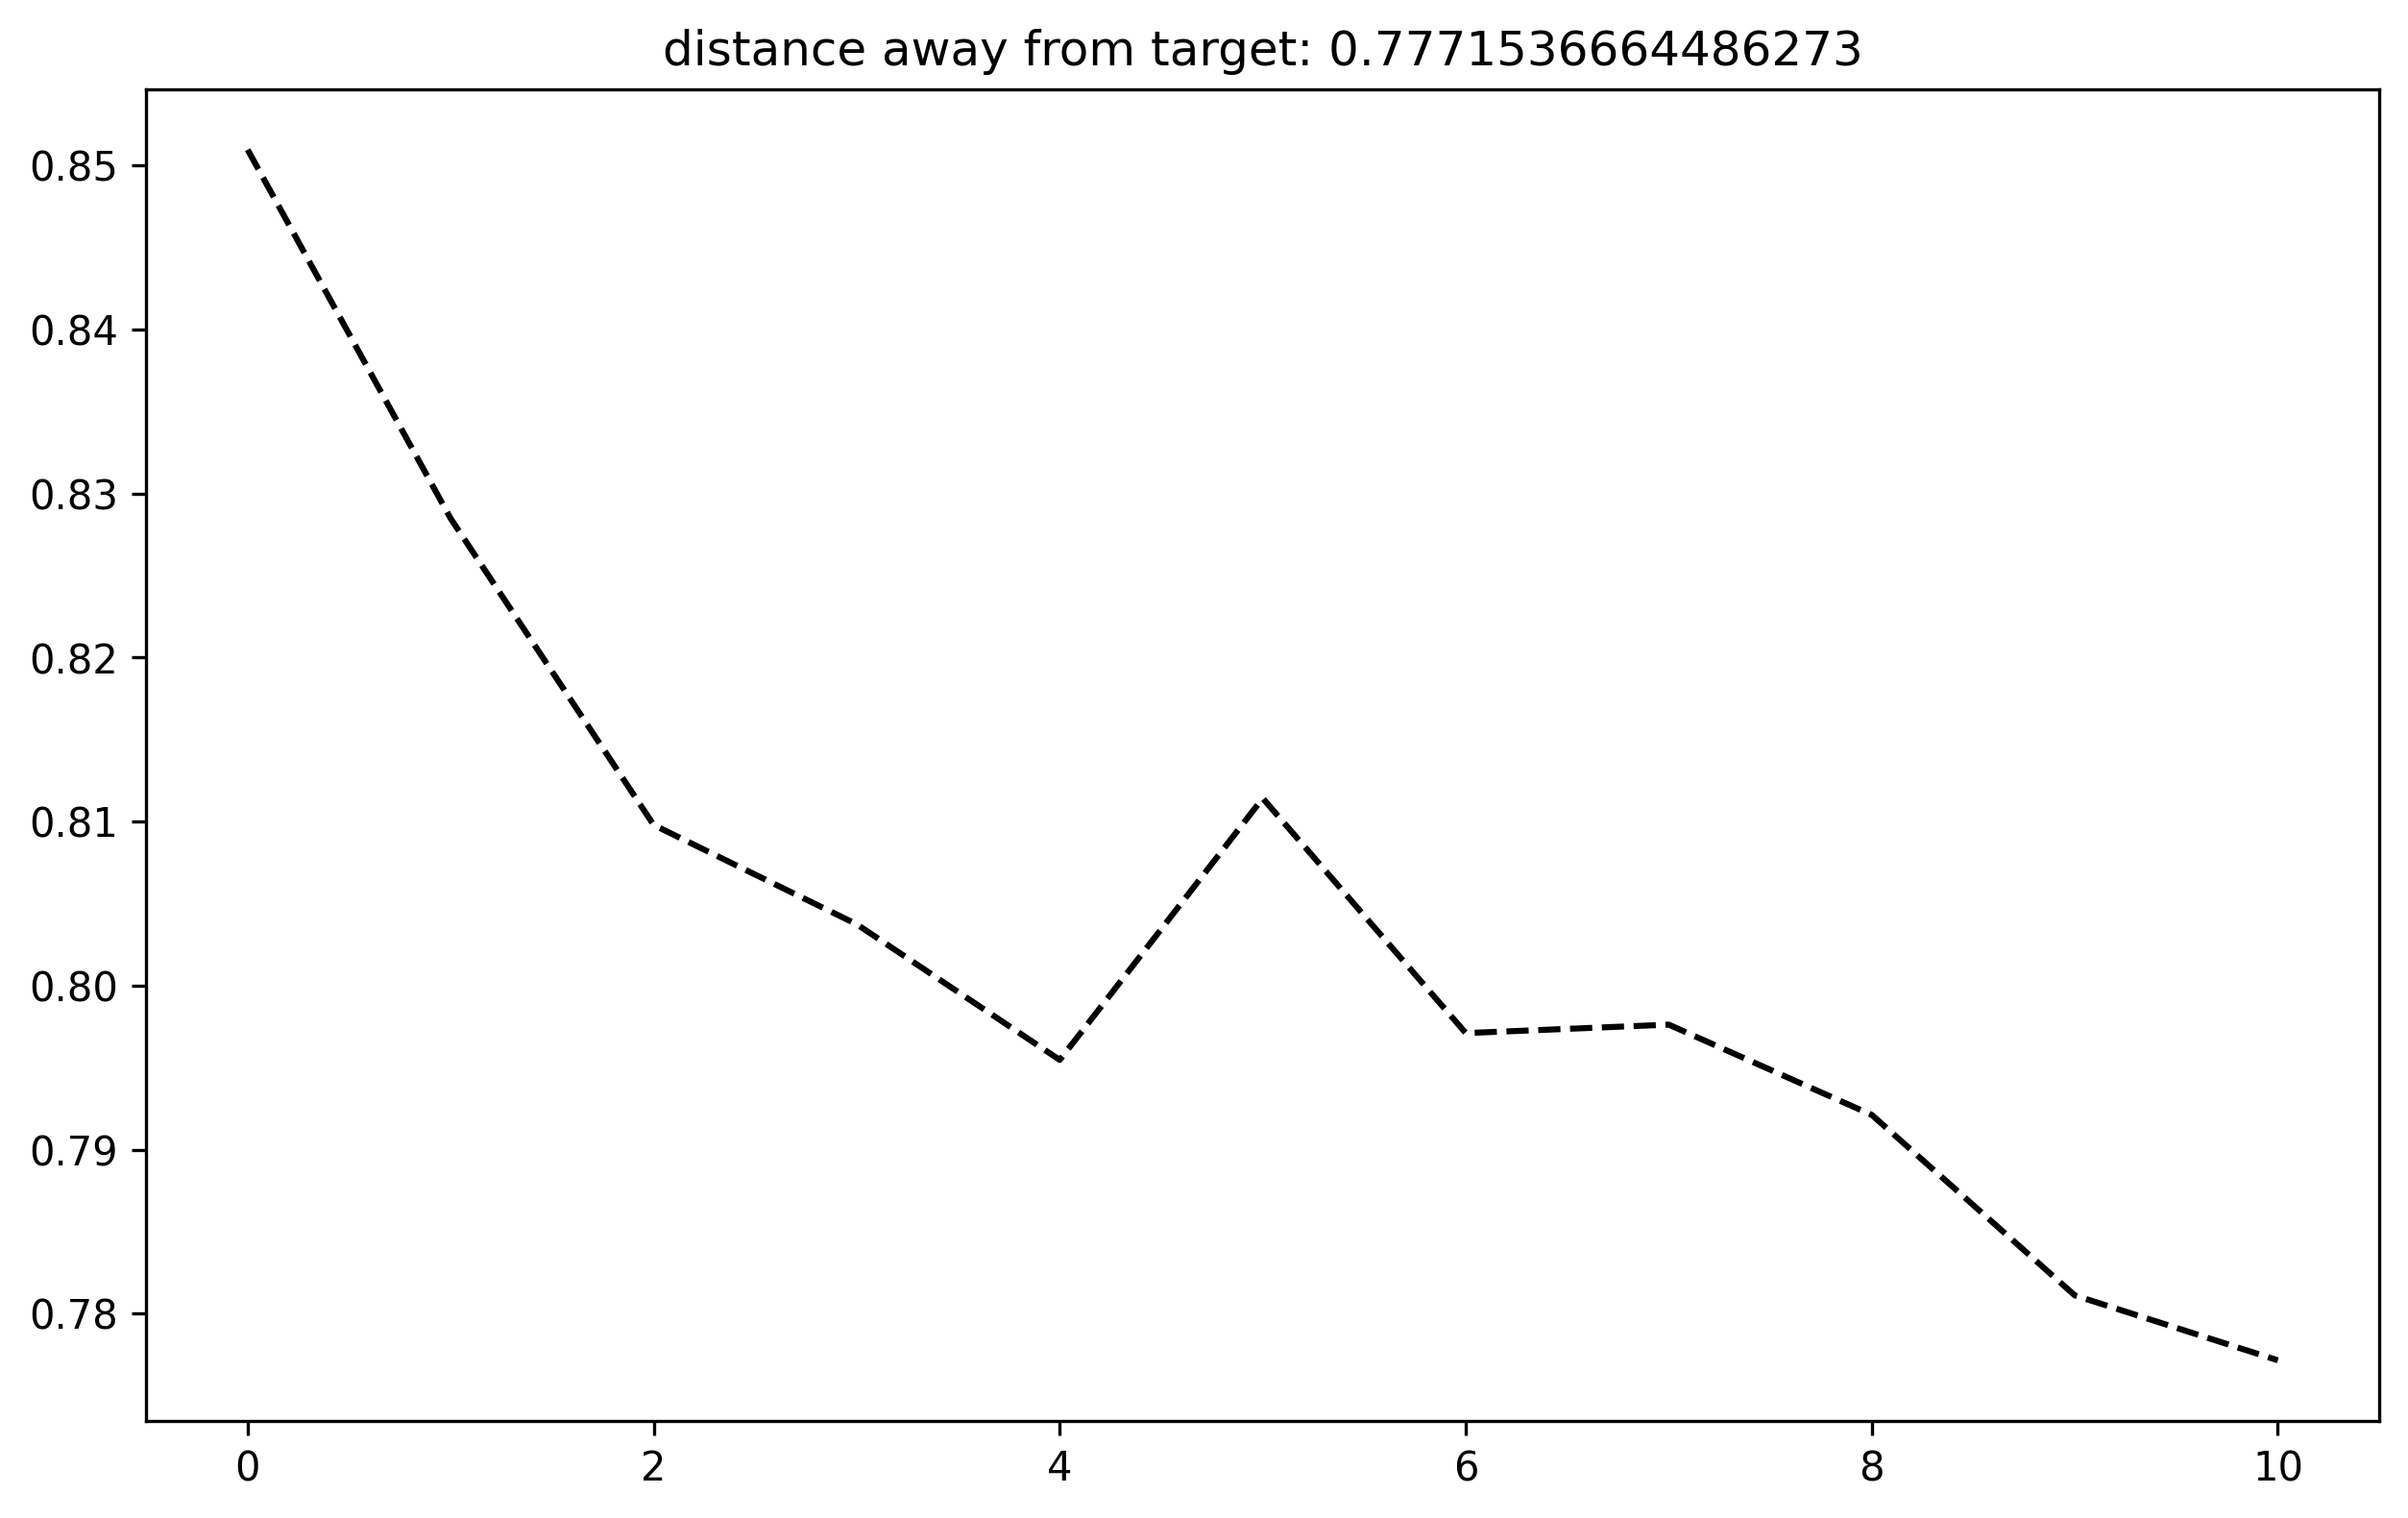
\includegraphics[width=\textwidth]{figures/unfiltered/svm_custom_7.png}
		\caption*{AGT (Unfiltered): 7×7m}
	\end{minipage}
\end{figure}

\begin{figure}[H]
	\centering
	\begin{minipage}{0.49\textwidth}
		\centering
		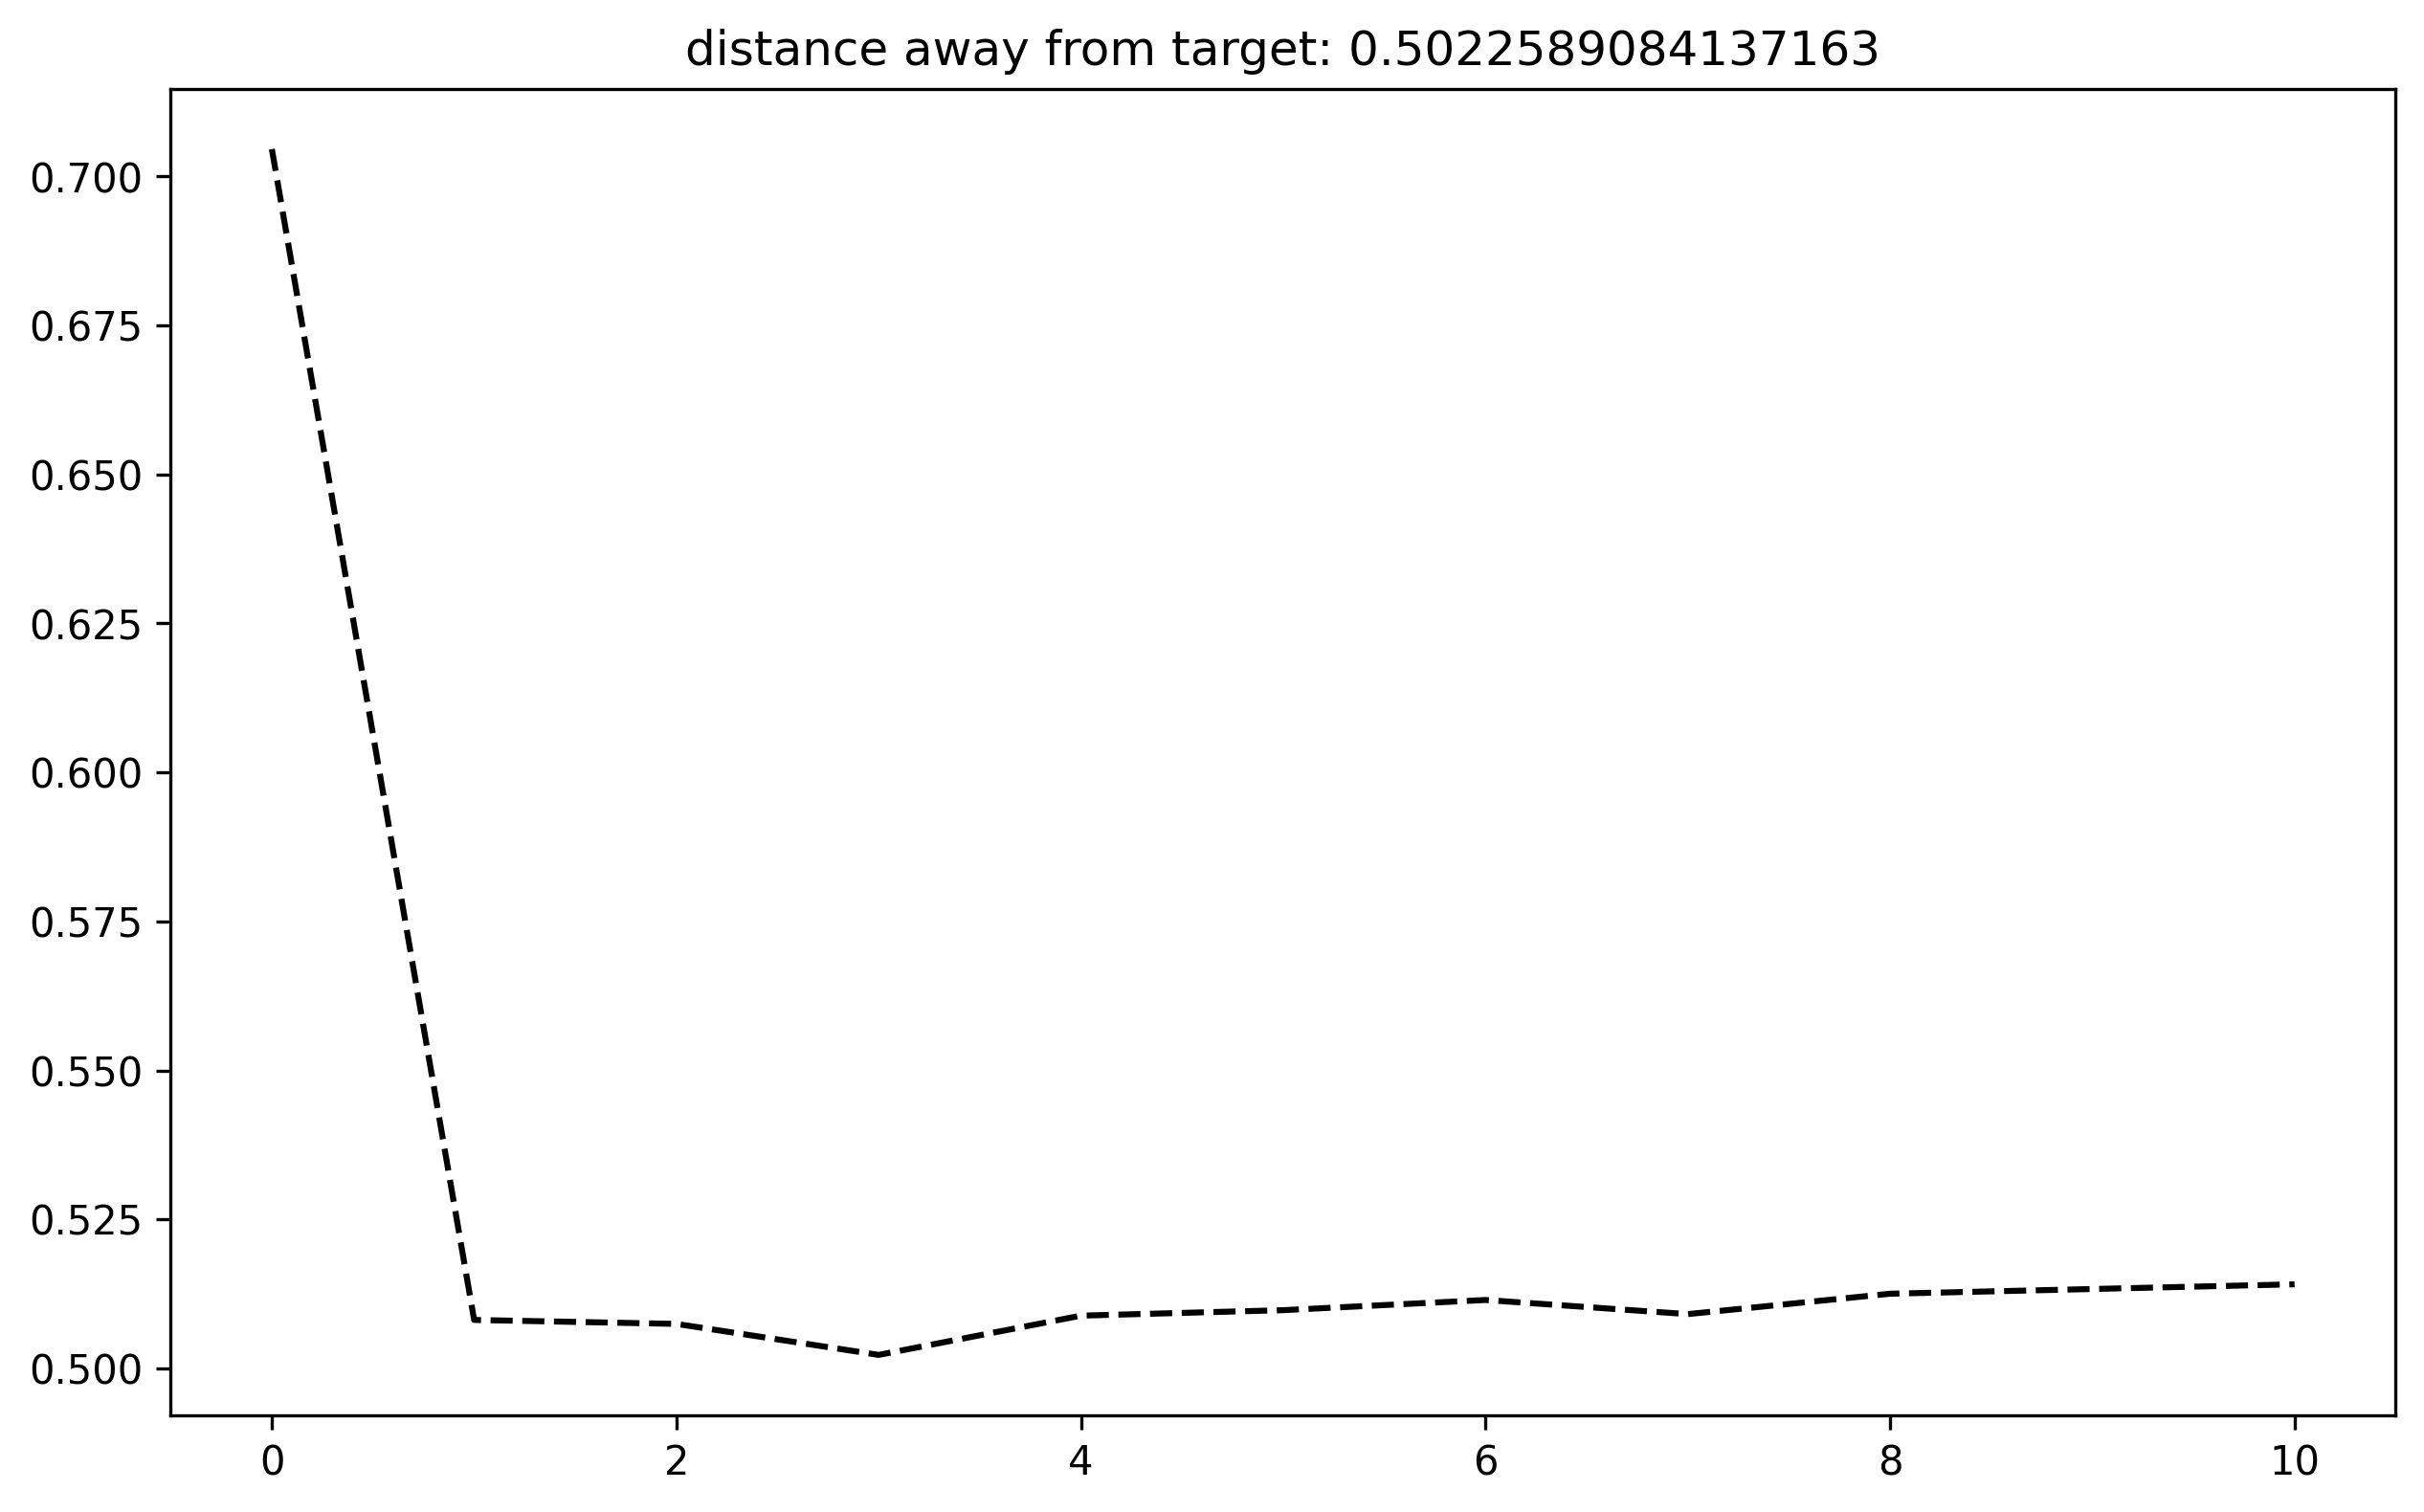
\includegraphics[width=\textwidth]{figures/filtered/svm_custom_15.png}
		\caption*{AGT (Filtered): 15×15m}
	\end{minipage}
	\hfill
	\begin{minipage}{0.49\textwidth}
		\centering
		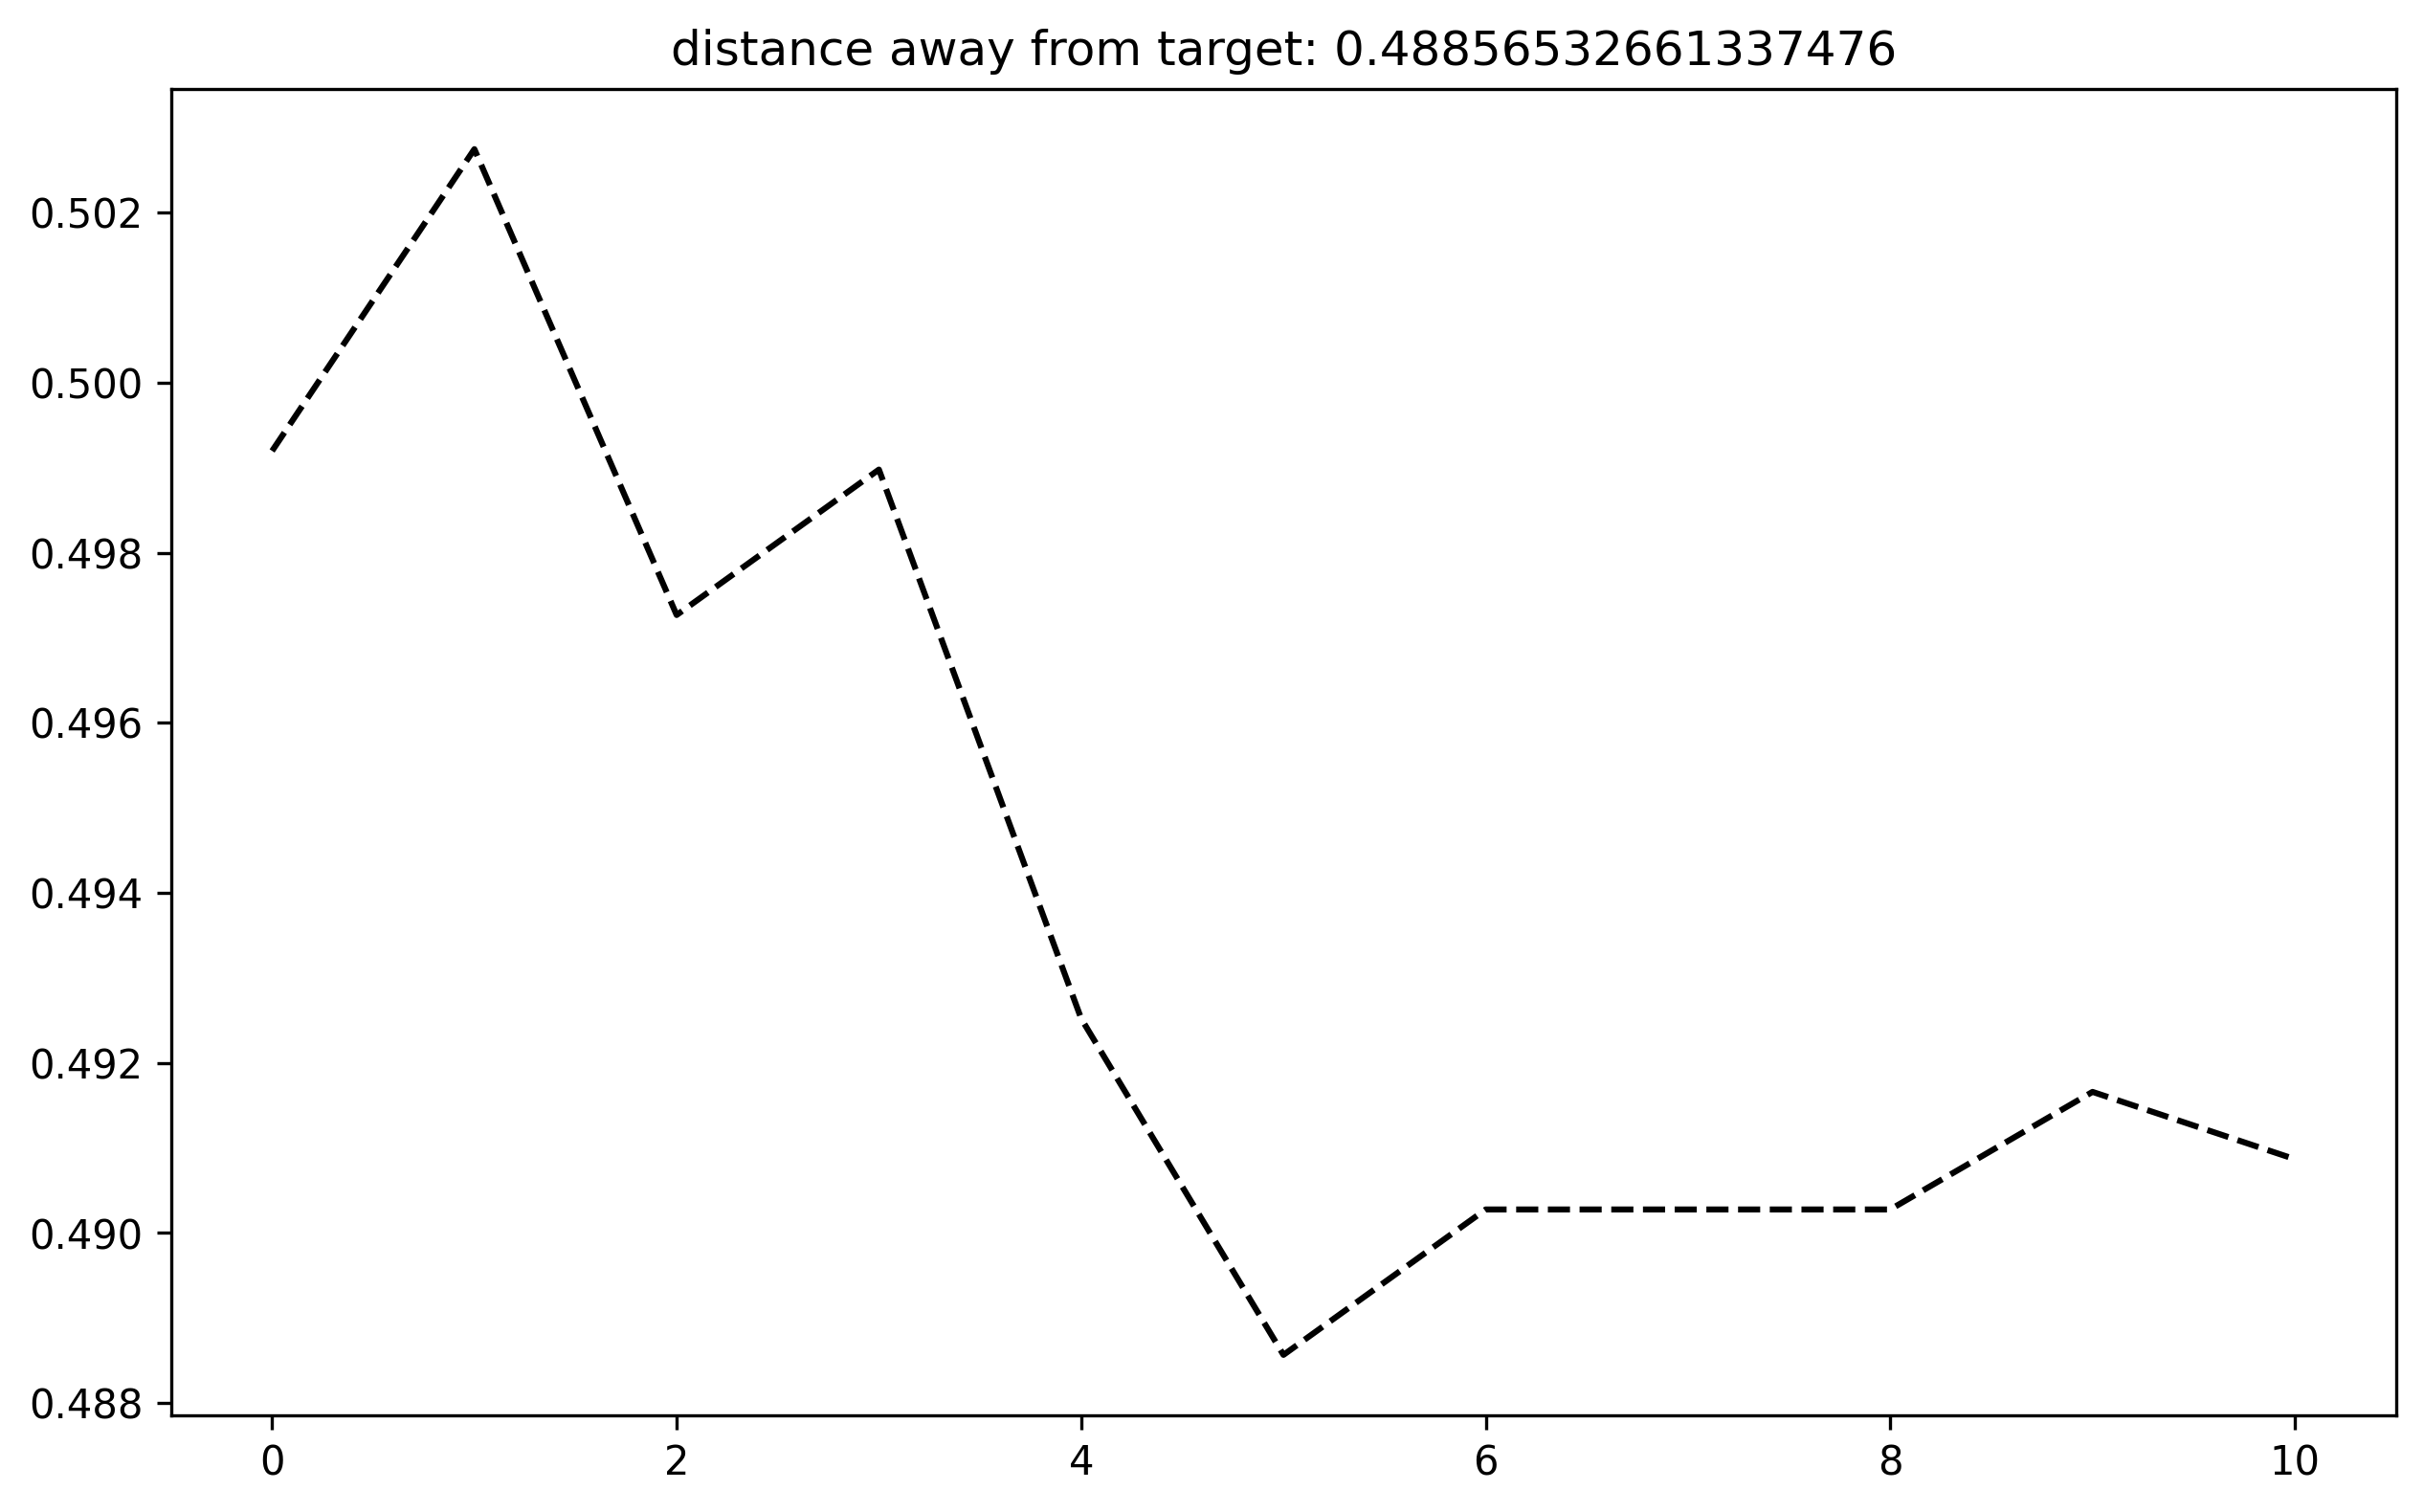
\includegraphics[width=\textwidth]{figures/unfiltered/svm_custom_15.png}
		\caption*{AGT (Unfiltered): 15×15m}
	\end{minipage}
\end{figure}

\clearpage

\subsection*{XGBoost}

\begin{figure}[H]
	\centering
	\begin{minipage}{0.49\textwidth}
		\centering
		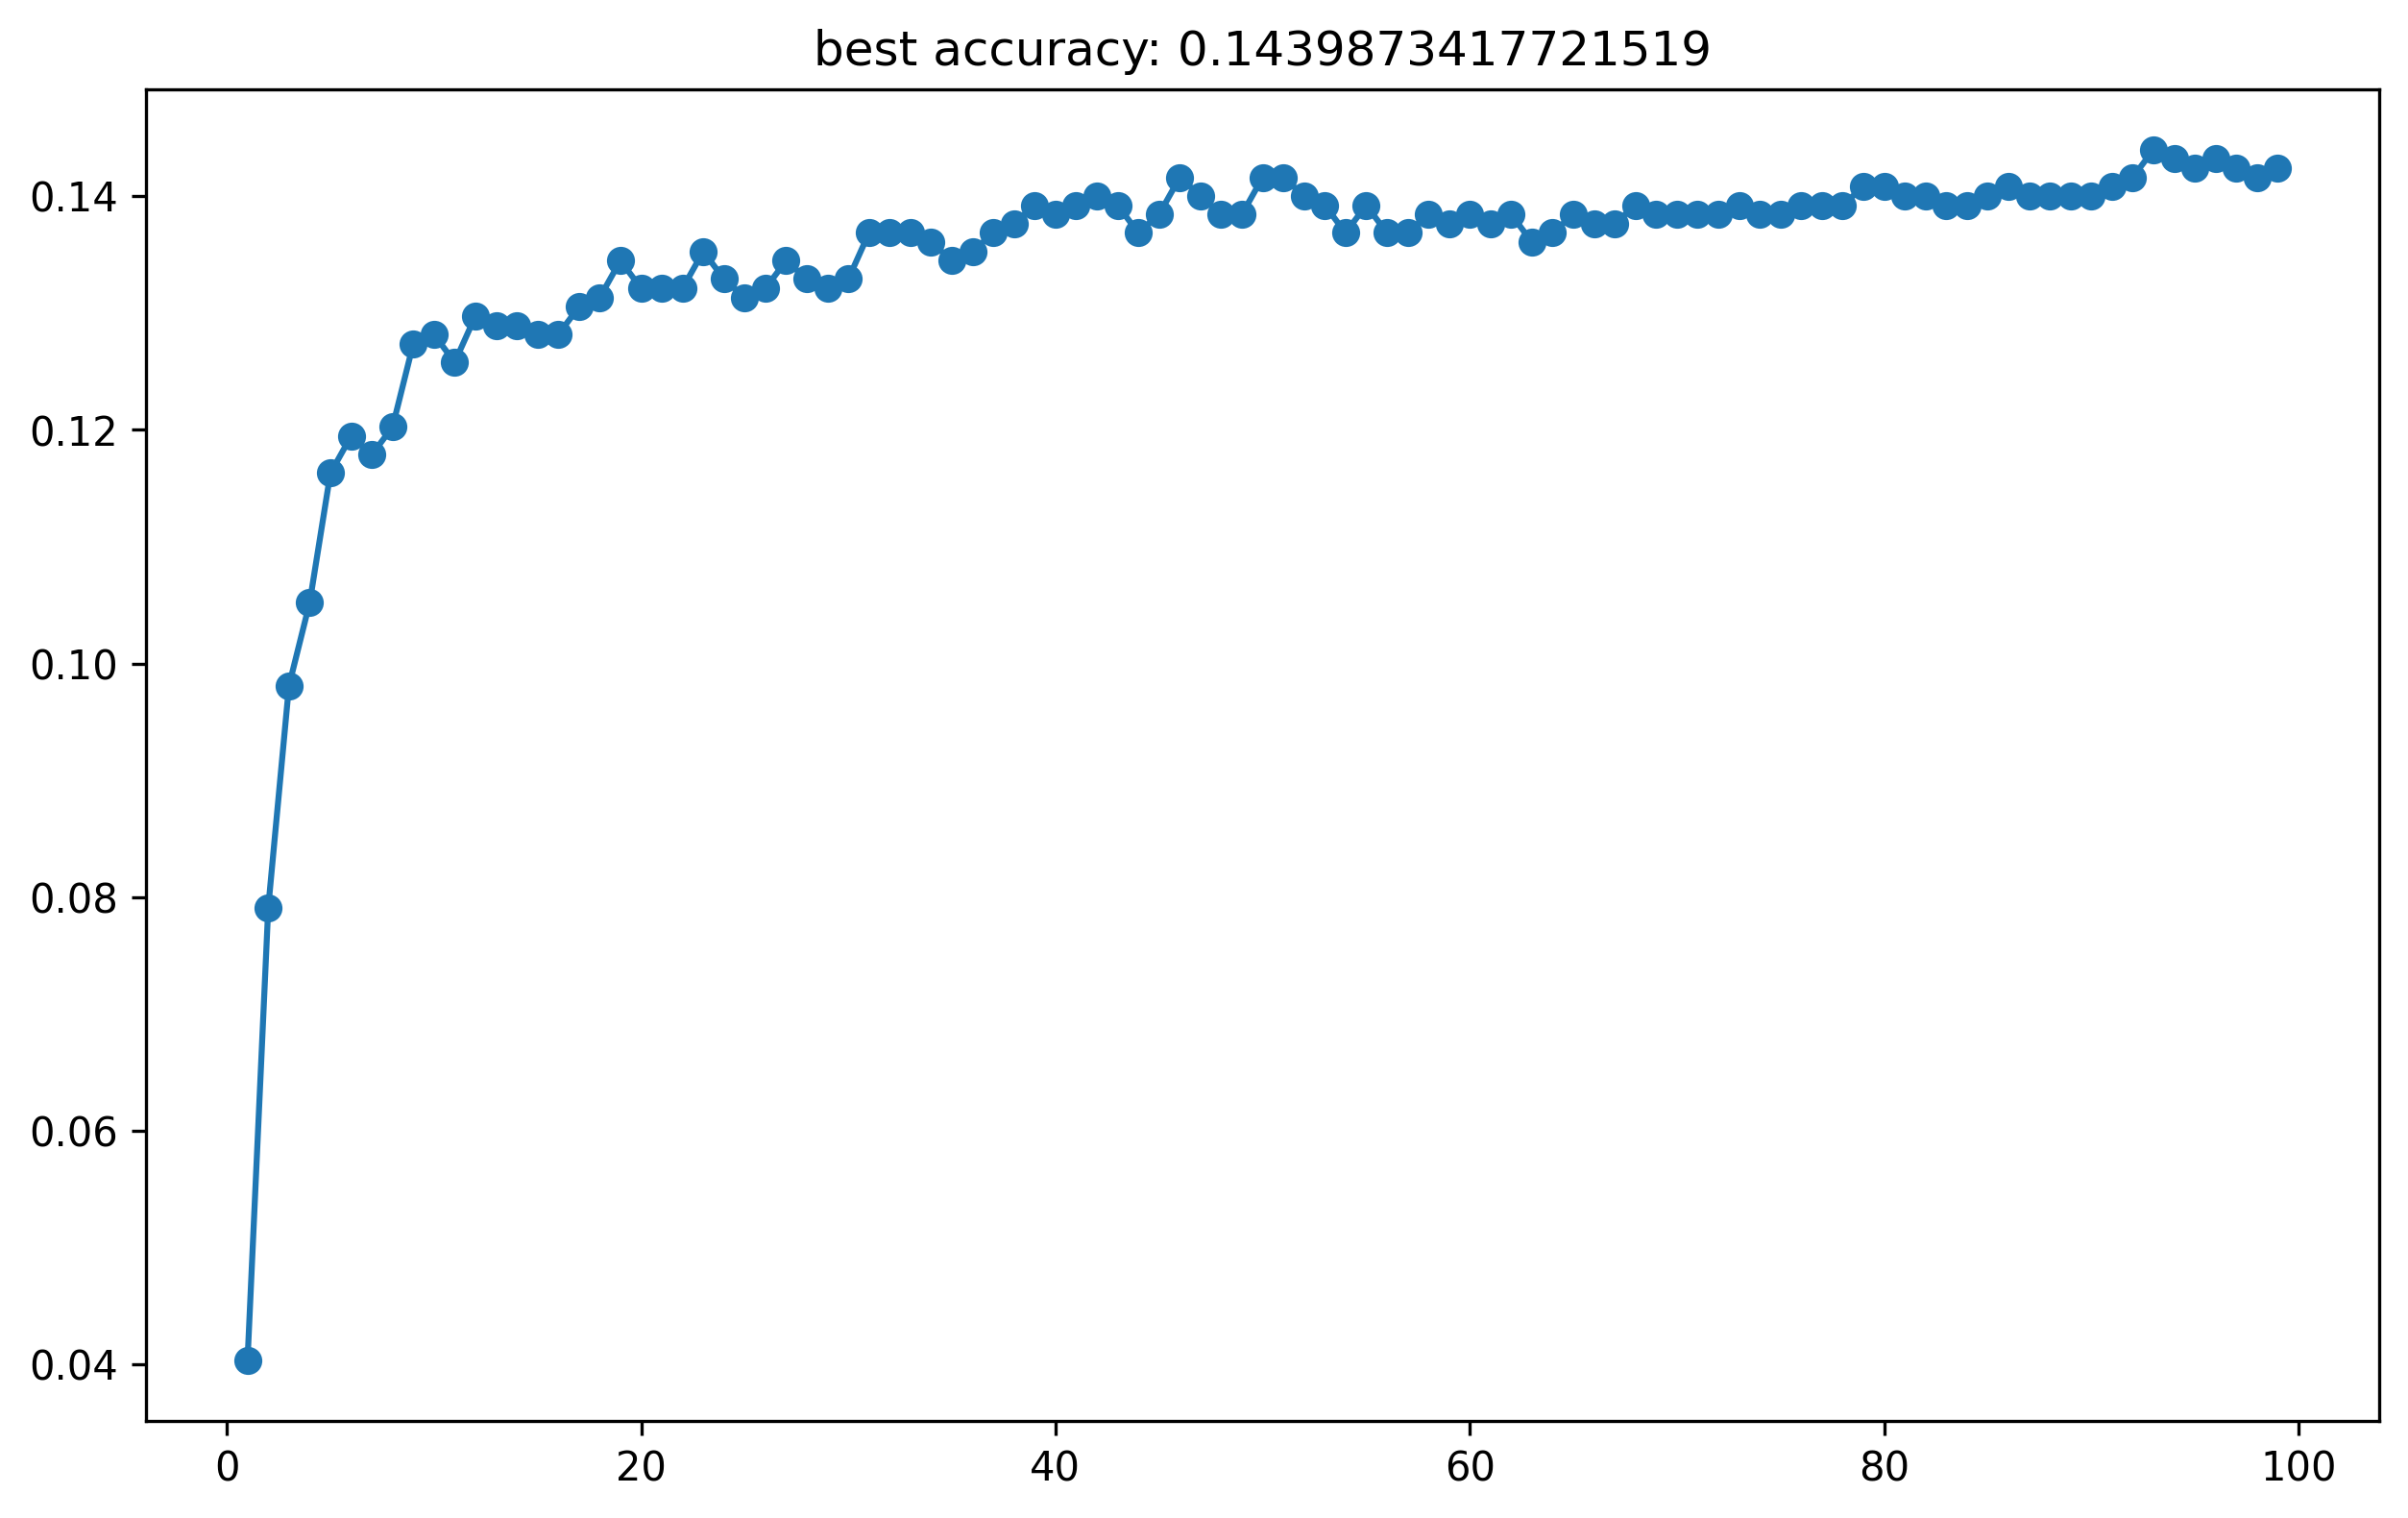
\includegraphics[width=\textwidth]{figures/filtered/xgb_softmax_acc_1.png}
		\caption*{Accuracy (Filtered): 1×1m}
	\end{minipage}
	\hfill
	\begin{minipage}{0.49\textwidth}
		\centering
		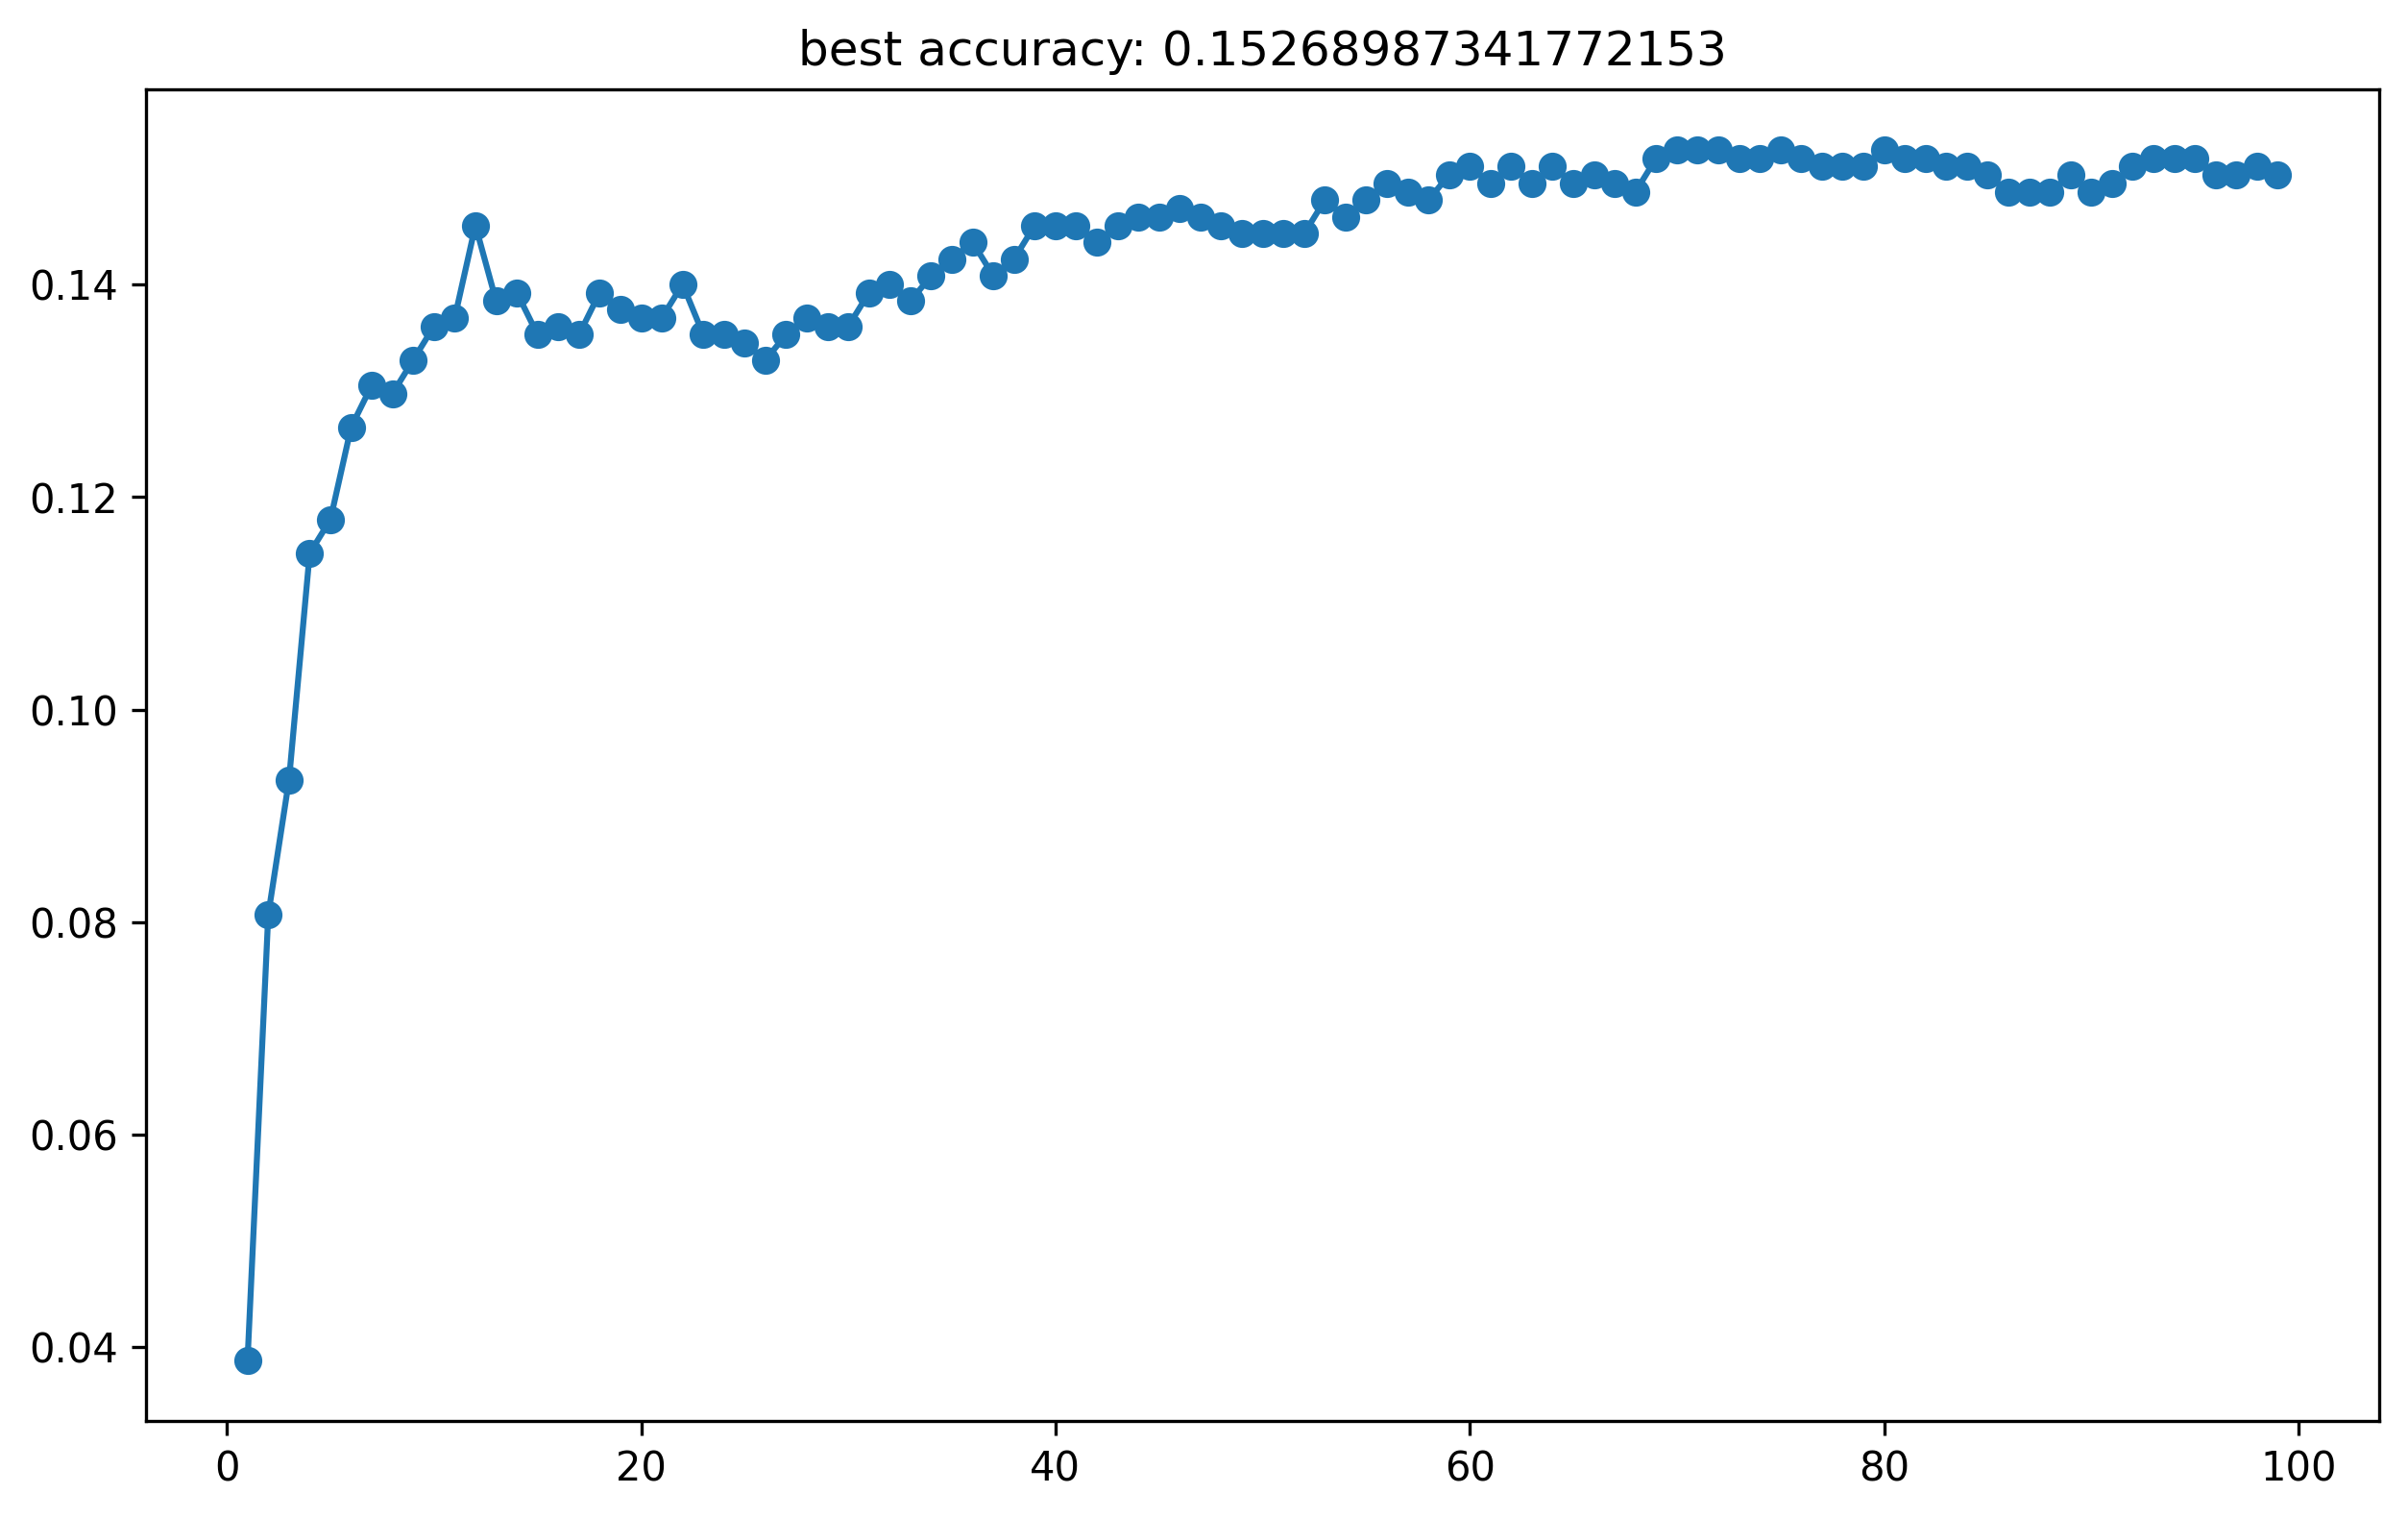
\includegraphics[width=\textwidth]{figures/unfiltered/xgb_softmax_acc_1.png}
		\caption*{Accuracy (Unfiltered): 1×1m}
	\end{minipage}
\end{figure}

\begin{figure}[H]
	\centering
	\begin{minipage}{0.49\textwidth}
		\centering
		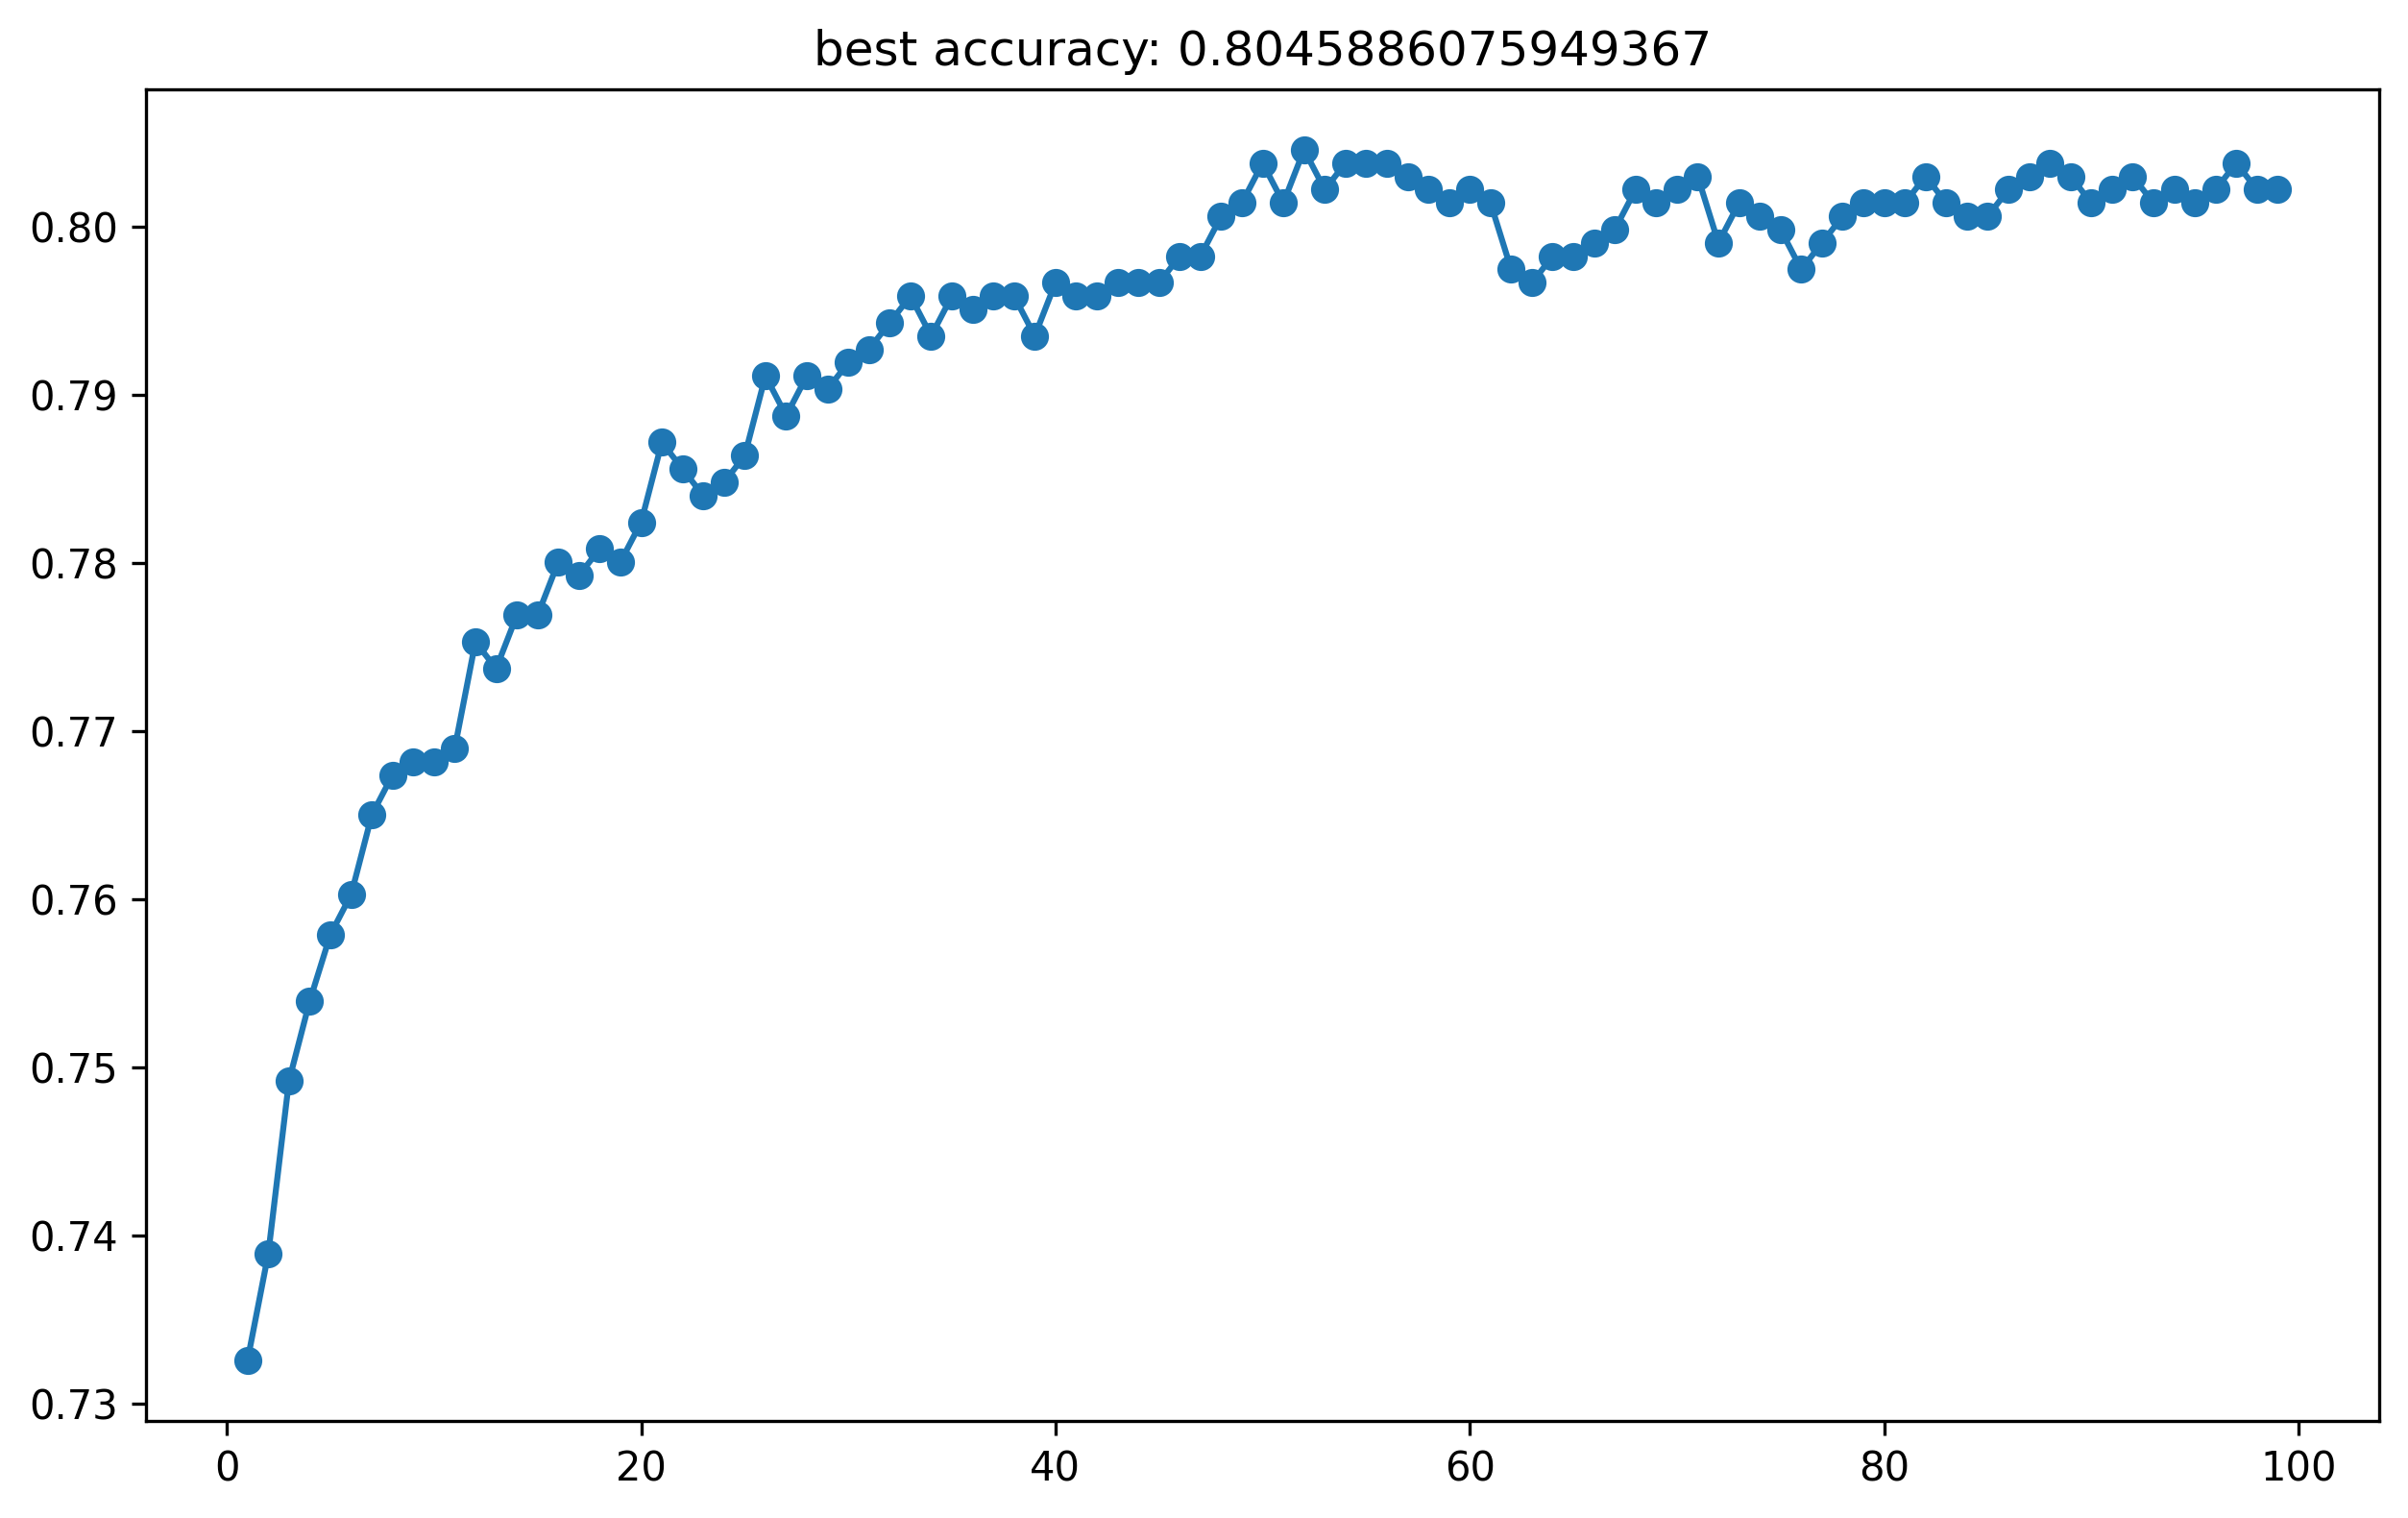
\includegraphics[width=\textwidth]{figures/filtered/xgb_softmax_acc_7.png}
		\caption*{Accuracy (Filtered): 7×7m}
	\end{minipage}
	\hfill
	\begin{minipage}{0.49\textwidth}
		\centering
		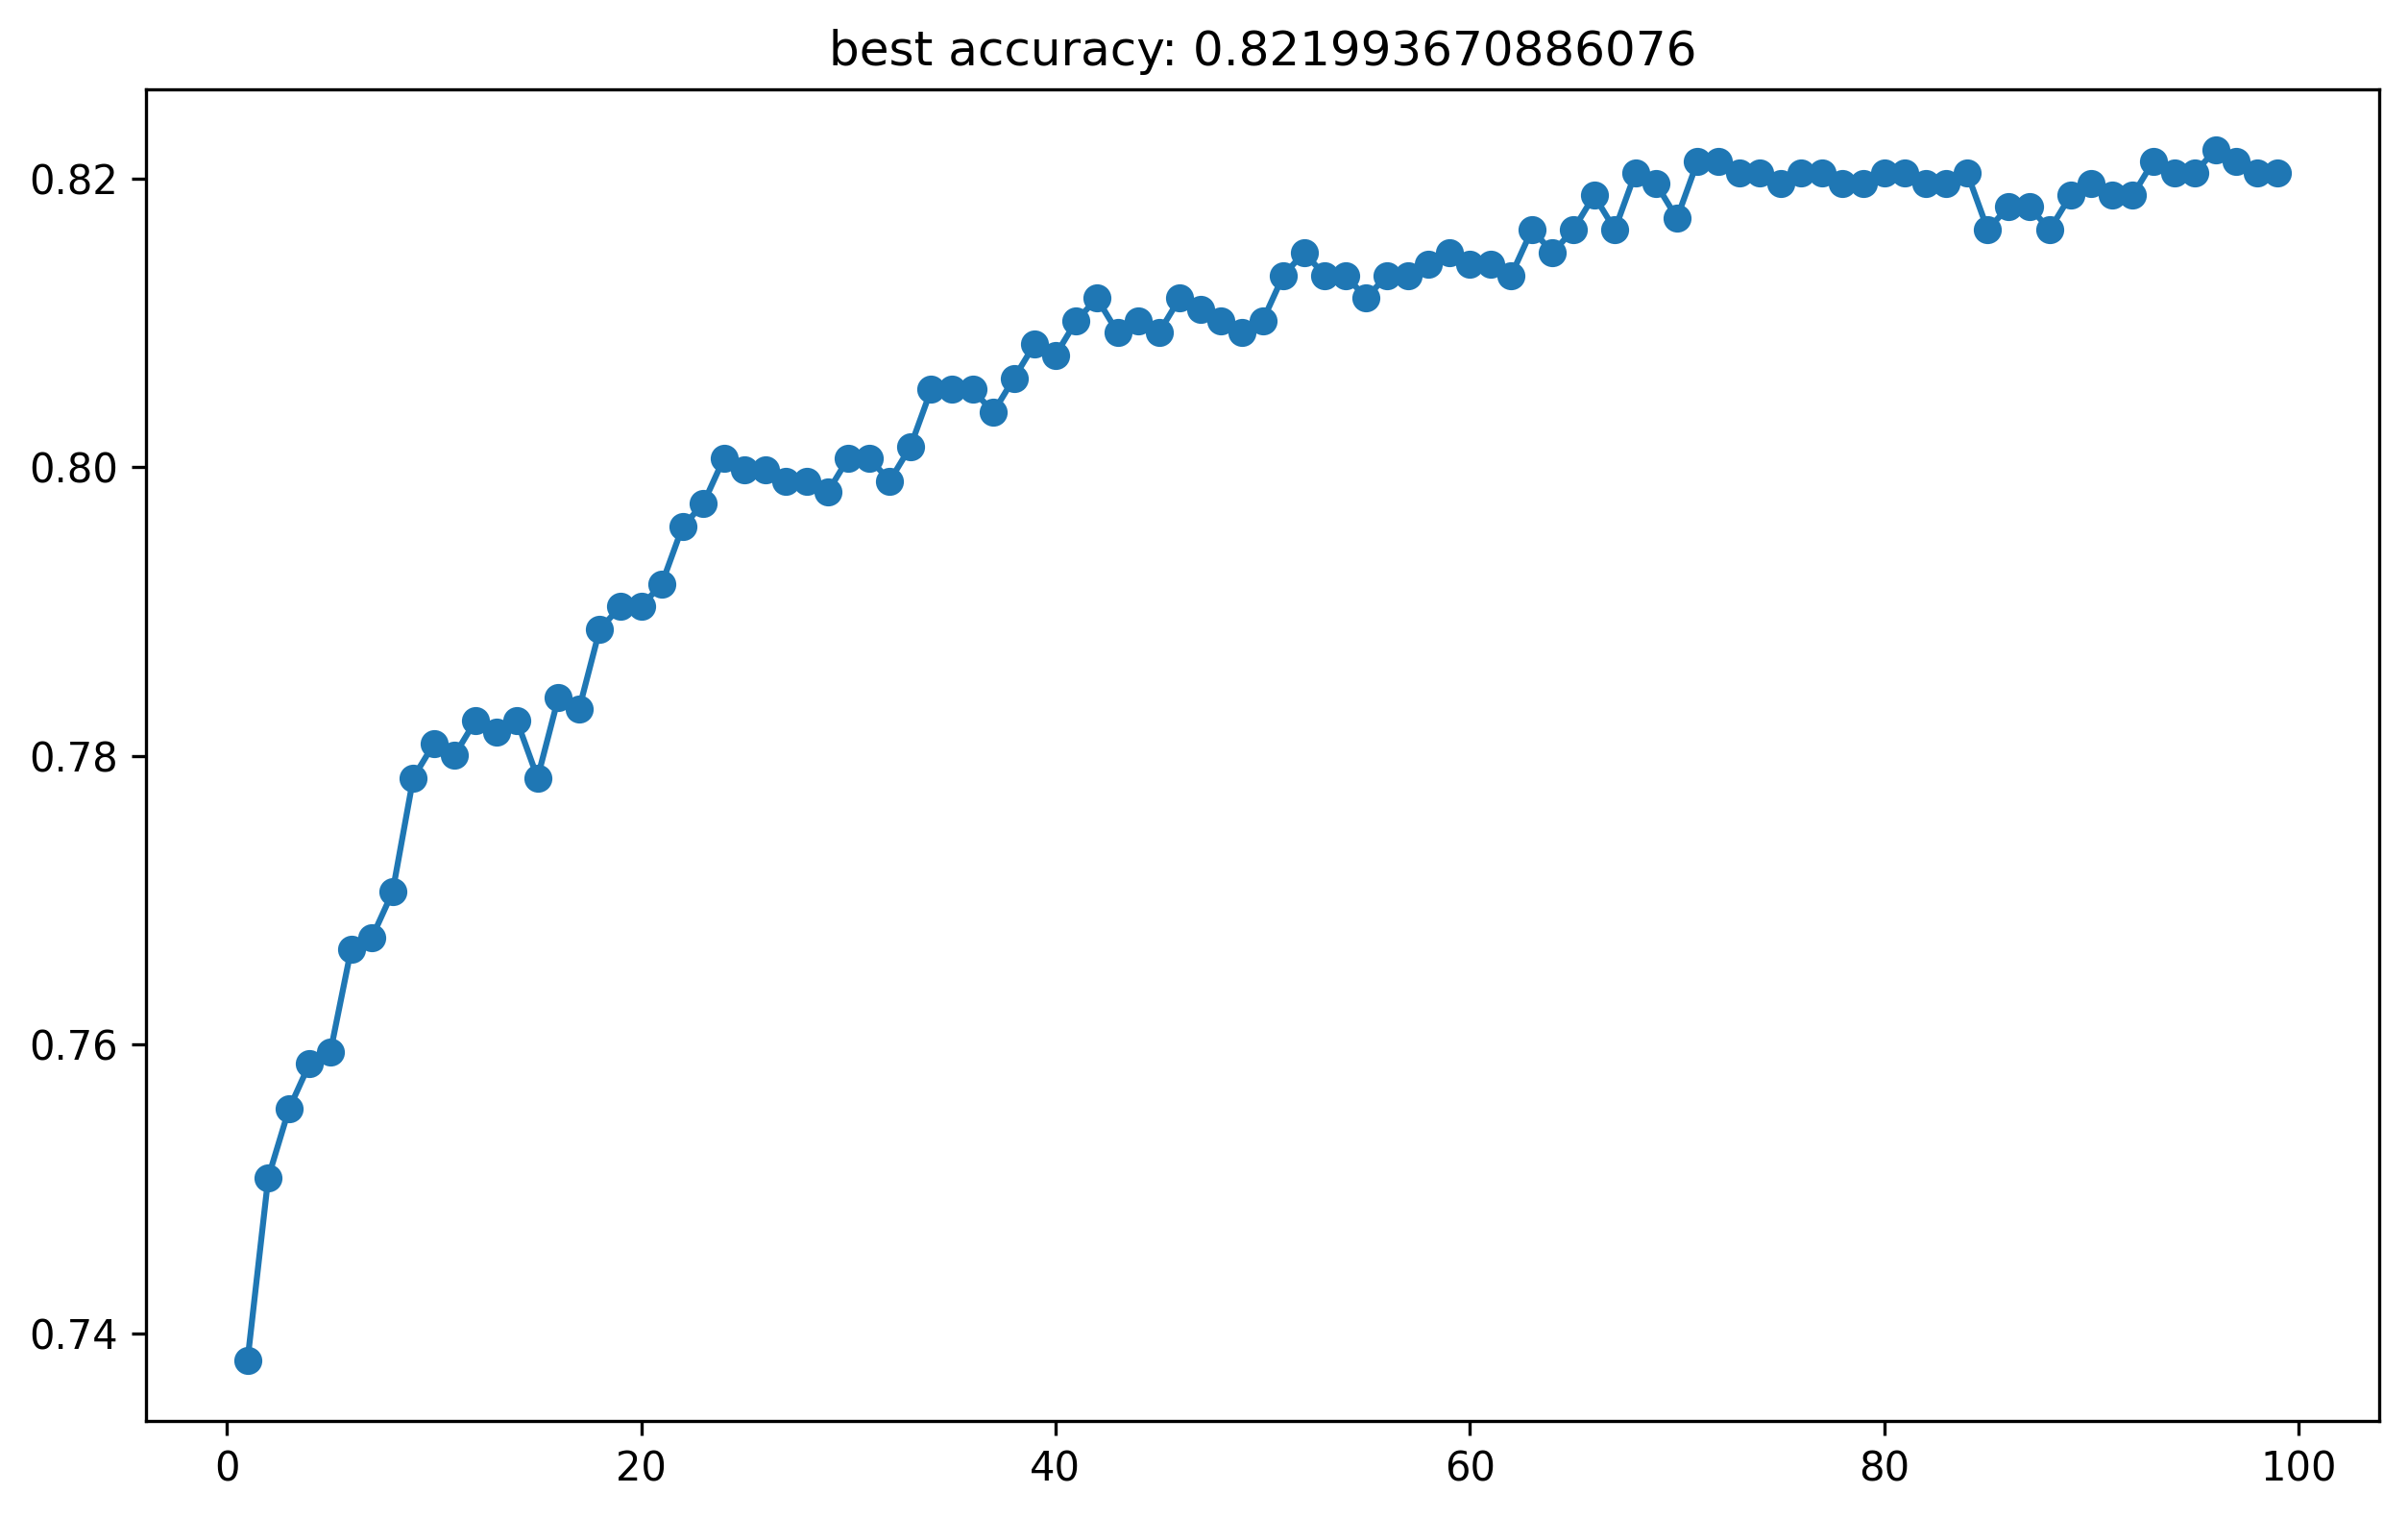
\includegraphics[width=\textwidth]{figures/unfiltered/xgb_softmax_acc_7.png}
		\caption*{Accuracy (Unfiltered): 7×7m}
	\end{minipage}
\end{figure}

\begin{figure}[H]
	\centering
	\begin{minipage}{0.49\textwidth}
		\centering
		\includegraphics[width=\textwidth]{figures/filtered/xgb_softmax_acc_15.png}
		\caption*{Accuracy (Filtered): 15×15m}
	\end{minipage}
	\hfill
	\begin{minipage}{0.49\textwidth}
		\centering
		\includegraphics[width=\textwidth]{figures/unfiltered/xgb_softmax_acc_15.png}
		\caption*{Accuracy (Unfiltered): 15×15m}
	\end{minipage}
\end{figure}

\begin{figure}[H]
	\centering
	\begin{minipage}{0.49\textwidth}
		\centering
		\includegraphics[width=\textwidth]{figures/filtered/xgb_softmax_custom_1.png}
		\caption*{AGT (Filtered): 1×1m}
	\end{minipage}
	\hfill
	\begin{minipage}{0.49\textwidth}
		\centering
		\includegraphics[width=\textwidth]{figures/unfiltered/xgb_softmax_custom_1.png}
		\caption*{AGT (Unfiltered): 1×1m}
	\end{minipage}
\end{figure}

\begin{figure}[H]
	\centering
	\begin{minipage}{0.49\textwidth}
		\centering
		\includegraphics[width=\textwidth]{figures/filtered/xgb_softmax_custom_7.png}
		\caption*{AGT (Filtered): 7×7m}
	\end{minipage}
	\hfill
	\begin{minipage}{0.49\textwidth}
		\centering
		\includegraphics[width=\textwidth]{figures/unfiltered/xgb_softmax_custom_7.png}
		\caption*{AGT (Unfiltered): 7×7m}
	\end{minipage}
\end{figure}

\begin{figure}[H]
	\centering
	\begin{minipage}{0.49\textwidth}
		\centering
		\includegraphics[width=\textwidth]{figures/filtered/xgb_softmax_custom_15.png}
		\caption*{AGT (Filtered): 15×15m}
	\end{minipage}
	\hfill
	\begin{minipage}{0.49\textwidth}
		\centering
		\includegraphics[width=\textwidth]{figures/unfiltered/xgb_softmax_custom_15.png}
		\caption*{AGT (Unfiltered): 15×15m}
	\end{minipage}
\end{figure}

\clearpage

\subsection*{XGBoost Random Forest}

\begin{figure}[H]
	\centering
	\begin{minipage}{0.49\textwidth}
		\centering
		\includegraphics[width=\textwidth]{figures/filtered/xgbrf_acc_1.png}
		\caption*{Accuracy (Filtered): 1×1m}
	\end{minipage}
	\hfill
	\begin{minipage}{0.49\textwidth}
		\centering
		\includegraphics[width=\textwidth]{figures/unfiltered/xgbrf_acc_1.png}
		\caption*{Accuracy (Unfiltered): 1×1m}
	\end{minipage}
\end{figure}

\begin{figure}[H]
	\centering
	\begin{minipage}{0.49\textwidth}
		\centering
		\includegraphics[width=\textwidth]{figures/filtered/xgbrf_acc_7.png}
		\caption*{Accuracy (Filtered): 7×7m}
	\end{minipage}
	\hfill
	\begin{minipage}{0.49\textwidth}
		\centering
		\includegraphics[width=\textwidth]{figures/unfiltered/xgbrf_acc_7.png}
		\caption*{Accuracy (Unfiltered): 7×7m}
	\end{minipage}
\end{figure}

\begin{figure}[H]
	\centering
	\begin{minipage}{0.49\textwidth}
		\centering
		\includegraphics[width=\textwidth]{figures/filtered/xgbrf_acc_15.png}
		\caption*{Accuracy (Filtered): 15×15m}
	\end{minipage}
	\hfill
	\begin{minipage}{0.49\textwidth}
		\centering
		\includegraphics[width=\textwidth]{figures/unfiltered/xgbrf_acc_15.png}
		\caption*{Accuracy (Unfiltered): 15×15m}
	\end{minipage}
\end{figure}

\begin{figure}[H]
	\centering
	\begin{minipage}{0.49\textwidth}
		\centering
		\includegraphics[width=\textwidth]{figures/filtered/xgbrf_custom_1.png}
		\caption*{AGT (Filtered): 1×1m}
	\end{minipage}
	\hfill
	\begin{minipage}{0.49\textwidth}
		\centering
		\includegraphics[width=\textwidth]{figures/unfiltered/xgbrf_custom_1.png}
		\caption*{AGT (Unfiltered): 1×1m}
	\end{minipage}
\end{figure}

\begin{figure}[H]
	\centering
	\begin{minipage}{0.49\textwidth}
		\centering
		\includegraphics[width=\textwidth]{figures/filtered/xgbrf_custom_7.png}
		\caption*{AGT (Filtered): 7×7m}
	\end{minipage}
	\hfill
	\begin{minipage}{0.49\textwidth}
		\centering
		\includegraphics[width=\textwidth]{figures/unfiltered/xgbrf_custom_7.png}
		\caption*{AGT (Unfiltered): 7×7m}
	\end{minipage}
\end{figure}

\begin{figure}[H]
	\centering
	\begin{minipage}{0.49\textwidth}
		\centering
		\includegraphics[width=\textwidth]{figures/filtered/xgbrf_custom_15.png}
		\caption*{AGT (Filtered): 15×15m}
	\end{minipage}
	\hfill
	\begin{minipage}{0.49\textwidth}
		\centering
		\includegraphics[width=\textwidth]{figures/unfiltered/xgbrf_custom_15.png}
		\caption*{AGT (Unfiltered): 15×15m}
	\end{minipage}
\end{figure}


\end{document}
